% Options for packages loaded elsewhere
\PassOptionsToPackage{unicode}{hyperref}
\PassOptionsToPackage{hyphens}{url}
%
\documentclass[
]{book}
\usepackage{amsmath,amssymb}
\usepackage{iftex}
\ifPDFTeX
  \usepackage[T1]{fontenc}
  \usepackage[utf8]{inputenc}
  \usepackage{textcomp} % provide euro and other symbols
\else % if luatex or xetex
  \usepackage{unicode-math} % this also loads fontspec
  \defaultfontfeatures{Scale=MatchLowercase}
  \defaultfontfeatures[\rmfamily]{Ligatures=TeX,Scale=1}
\fi
\usepackage{lmodern}
\ifPDFTeX\else
  % xetex/luatex font selection
\fi
% Use upquote if available, for straight quotes in verbatim environments
\IfFileExists{upquote.sty}{\usepackage{upquote}}{}
\IfFileExists{microtype.sty}{% use microtype if available
  \usepackage[]{microtype}
  \UseMicrotypeSet[protrusion]{basicmath} % disable protrusion for tt fonts
}{}
\makeatletter
\@ifundefined{KOMAClassName}{% if non-KOMA class
  \IfFileExists{parskip.sty}{%
    \usepackage{parskip}
  }{% else
    \setlength{\parindent}{0pt}
    \setlength{\parskip}{6pt plus 2pt minus 1pt}}
}{% if KOMA class
  \KOMAoptions{parskip=half}}
\makeatother
\usepackage{xcolor}
\usepackage{color}
\usepackage{fancyvrb}
\newcommand{\VerbBar}{|}
\newcommand{\VERB}{\Verb[commandchars=\\\{\}]}
\DefineVerbatimEnvironment{Highlighting}{Verbatim}{commandchars=\\\{\}}
% Add ',fontsize=\small' for more characters per line
\usepackage{framed}
\definecolor{shadecolor}{RGB}{248,248,248}
\newenvironment{Shaded}{\begin{snugshade}}{\end{snugshade}}
\newcommand{\AlertTok}[1]{\textcolor[rgb]{0.94,0.16,0.16}{#1}}
\newcommand{\AnnotationTok}[1]{\textcolor[rgb]{0.56,0.35,0.01}{\textbf{\textit{#1}}}}
\newcommand{\AttributeTok}[1]{\textcolor[rgb]{0.13,0.29,0.53}{#1}}
\newcommand{\BaseNTok}[1]{\textcolor[rgb]{0.00,0.00,0.81}{#1}}
\newcommand{\BuiltInTok}[1]{#1}
\newcommand{\CharTok}[1]{\textcolor[rgb]{0.31,0.60,0.02}{#1}}
\newcommand{\CommentTok}[1]{\textcolor[rgb]{0.56,0.35,0.01}{\textit{#1}}}
\newcommand{\CommentVarTok}[1]{\textcolor[rgb]{0.56,0.35,0.01}{\textbf{\textit{#1}}}}
\newcommand{\ConstantTok}[1]{\textcolor[rgb]{0.56,0.35,0.01}{#1}}
\newcommand{\ControlFlowTok}[1]{\textcolor[rgb]{0.13,0.29,0.53}{\textbf{#1}}}
\newcommand{\DataTypeTok}[1]{\textcolor[rgb]{0.13,0.29,0.53}{#1}}
\newcommand{\DecValTok}[1]{\textcolor[rgb]{0.00,0.00,0.81}{#1}}
\newcommand{\DocumentationTok}[1]{\textcolor[rgb]{0.56,0.35,0.01}{\textbf{\textit{#1}}}}
\newcommand{\ErrorTok}[1]{\textcolor[rgb]{0.64,0.00,0.00}{\textbf{#1}}}
\newcommand{\ExtensionTok}[1]{#1}
\newcommand{\FloatTok}[1]{\textcolor[rgb]{0.00,0.00,0.81}{#1}}
\newcommand{\FunctionTok}[1]{\textcolor[rgb]{0.13,0.29,0.53}{\textbf{#1}}}
\newcommand{\ImportTok}[1]{#1}
\newcommand{\InformationTok}[1]{\textcolor[rgb]{0.56,0.35,0.01}{\textbf{\textit{#1}}}}
\newcommand{\KeywordTok}[1]{\textcolor[rgb]{0.13,0.29,0.53}{\textbf{#1}}}
\newcommand{\NormalTok}[1]{#1}
\newcommand{\OperatorTok}[1]{\textcolor[rgb]{0.81,0.36,0.00}{\textbf{#1}}}
\newcommand{\OtherTok}[1]{\textcolor[rgb]{0.56,0.35,0.01}{#1}}
\newcommand{\PreprocessorTok}[1]{\textcolor[rgb]{0.56,0.35,0.01}{\textit{#1}}}
\newcommand{\RegionMarkerTok}[1]{#1}
\newcommand{\SpecialCharTok}[1]{\textcolor[rgb]{0.81,0.36,0.00}{\textbf{#1}}}
\newcommand{\SpecialStringTok}[1]{\textcolor[rgb]{0.31,0.60,0.02}{#1}}
\newcommand{\StringTok}[1]{\textcolor[rgb]{0.31,0.60,0.02}{#1}}
\newcommand{\VariableTok}[1]{\textcolor[rgb]{0.00,0.00,0.00}{#1}}
\newcommand{\VerbatimStringTok}[1]{\textcolor[rgb]{0.31,0.60,0.02}{#1}}
\newcommand{\WarningTok}[1]{\textcolor[rgb]{0.56,0.35,0.01}{\textbf{\textit{#1}}}}
\usepackage{longtable,booktabs,array}
\usepackage{calc} % for calculating minipage widths
% Correct order of tables after \paragraph or \subparagraph
\usepackage{etoolbox}
\makeatletter
\patchcmd\longtable{\par}{\if@noskipsec\mbox{}\fi\par}{}{}
\makeatother
% Allow footnotes in longtable head/foot
\IfFileExists{footnotehyper.sty}{\usepackage{footnotehyper}}{\usepackage{footnote}}
\makesavenoteenv{longtable}
\usepackage{graphicx}
\makeatletter
\def\maxwidth{\ifdim\Gin@nat@width>\linewidth\linewidth\else\Gin@nat@width\fi}
\def\maxheight{\ifdim\Gin@nat@height>\textheight\textheight\else\Gin@nat@height\fi}
\makeatother
% Scale images if necessary, so that they will not overflow the page
% margins by default, and it is still possible to overwrite the defaults
% using explicit options in \includegraphics[width, height, ...]{}
\setkeys{Gin}{width=\maxwidth,height=\maxheight,keepaspectratio}
% Set default figure placement to htbp
\makeatletter
\def\fps@figure{htbp}
\makeatother
\ifLuaTeX
  \usepackage{luacolor}
  \usepackage[soul]{lua-ul}
\else
  \usepackage{soul}
\fi
\setlength{\emergencystretch}{3em} % prevent overfull lines
\providecommand{\tightlist}{%
  \setlength{\itemsep}{0pt}\setlength{\parskip}{0pt}}
\setcounter{secnumdepth}{5}
% definitions for citeproc citations
\NewDocumentCommand\citeproctext{}{}
\NewDocumentCommand\citeproc{mm}{%
  \begingroup\def\citeproctext{#2}\cite{#1}\endgroup}
\makeatletter
 % allow citations to break across lines
 \let\@cite@ofmt\@firstofone
 % avoid brackets around text for \cite:
 \def\@biblabel#1{}
 \def\@cite#1#2{{#1\if@tempswa , #2\fi}}
\makeatother
\newlength{\cslhangindent}
\setlength{\cslhangindent}{1.5em}
\newlength{\csllabelwidth}
\setlength{\csllabelwidth}{3em}
\newenvironment{CSLReferences}[2] % #1 hanging-indent, #2 entry-spacing
 {\begin{list}{}{%
  \setlength{\itemindent}{0pt}
  \setlength{\leftmargin}{0pt}
  \setlength{\parsep}{0pt}
  % turn on hanging indent if param 1 is 1
  \ifodd #1
   \setlength{\leftmargin}{\cslhangindent}
   \setlength{\itemindent}{-1\cslhangindent}
  \fi
  % set entry spacing
  \setlength{\itemsep}{#2\baselineskip}}}
 {\end{list}}
\usepackage{calc}
\newcommand{\CSLBlock}[1]{\hfill\break\parbox[t]{\linewidth}{\strut\ignorespaces#1\strut}}
\newcommand{\CSLLeftMargin}[1]{\parbox[t]{\csllabelwidth}{\strut#1\strut}}
\newcommand{\CSLRightInline}[1]{\parbox[t]{\linewidth - \csllabelwidth}{\strut#1\strut}}
\newcommand{\CSLIndent}[1]{\hspace{\cslhangindent}#1}
\ifLuaTeX
  \usepackage{selnolig}  % disable illegal ligatures
\fi
\usepackage{bookmark}
\IfFileExists{xurl.sty}{\usepackage{xurl}}{} % add URL line breaks if available
\urlstyle{same}
\hypersetup{
  pdftitle={Happy Git and GitHub for the useR},
  pdfauthor={Jenny Bryan, the STAT 545 TAs, Jim Hester},
  hidelinks,
  pdfcreator={LaTeX via pandoc}}

\title{Happy Git and GitHub for the useR}
\author{Jenny Bryan, the STAT 545 TAs, Jim Hester}
\date{}

\begin{document}
\maketitle

{
\setcounter{tocdepth}{1}
\tableofcontents
}
\chapter*{Let's Git started}\label{lets-git-started}
\addcontentsline{toc}{chapter}{Let's Git started}

Still from Heaven King video

Happy Git provides opinionated instructions on how to:

\begin{itemize}
\tightlist
\item
  Install Git and get it working smoothly with GitHub, in the shell and in the \href{https://www.rstudio.com/products/rstudio/}{RStudio IDE}.
\item
  Develop a few key workflows that cover your most common tasks.
\item
  Integrate Git and GitHub into your daily work with R and \href{https://rmarkdown.rstudio.com}{R Markdown}.
\end{itemize}

The target reader is someone who uses R for data analysis or who works on R packages, although some of the content may be useful to those working in adjacent areas.

The first two parts, \hyperref[install-intro]{Installation} and \hyperref[connect-intro]{Connect Git, GitHub, RStudio}, provide a ``batteries included'' quick start to verify your setup.

In \hyperref[usage-intro]{Early GitHub Wins}, we rack up some early success with the basic workflows that are necessary to get your work onto GitHub. We also show the special synergy between R/R Markdown/RStudio and GitHub, which provides a powerful demonstration of why all this setup is worthwhile.

The use of Git/GitHub in data science has a slightly different vibe from that of pure software development, due to differences in the user's context and objective. Happy Git aims to complement existing, general Git resources by highlighting the most rewarding usage patterns for data science. This perspective on the Git landscape is presented in \hyperref[git-intro]{Basic Git Concepts} and \hyperref[workflows-intro]{Daily Workflows}.

\section*{License}\label{license}
\addcontentsline{toc}{section}{License}

{Happy Git and GitHub for the useR} by Jennifer Bryan is licensed under a Creative Commons Attribution-NonCommercial 4.0 International License.

\chapter{Why Git? Why GitHub?}\label{big-picture}

Why would a data analyst use hosted version control?

\emph{This intro has grown into a stand-alone article that is arguably a better introduction at this point. Until I merge it back in, consider reading the article instead: ``Excuse me, do you have a moment to talk about version control?'' \url{https://dx.doi.org/10.7287\%2Fpeerj.preprints.3159v2}.}

\section{Why Git?}\label{why-git}

\href{http://git-scm.com}{Git} is a \textbf{version control system}. Its original purpose was to help groups of developers work collaboratively on big software projects. Git manages the evolution of a set of files -- called a \textbf{repository} -- in a sane, highly structured way. If you have no idea what I'm talking about, think of it as the ``Track Changes'' features from Microsoft Word on steroids.

Git has been re-purposed by the data science community. In addition to using it for source code, we use it to manage the motley collection of files that make up typical data analytical projects, which often consist of data, figures, reports, and, yes, source code.

A solo data analyst, working on a single computer, will benefit from adopting version control. But not nearly enough to justify the pain of installation and workflow upheaval. There are much easier ways to get versioned back ups of your files, if that's all you're worried about.

In my opinion, \textbf{for new users}, the pros of Git only outweigh the cons when you factor in the overhead of communicating and collaborating with other people. Who among us does not need to do that? Your life is much easier if this is baked into your workflow, as opposed to being a separate process that you dread or neglect.

\section{Why GitHub?}\label{why-github}

This is where hosting services like \href{https://github.com}{GitHub}, \href{https://bitbucket.org}{Bitbucket}, and \href{https://about.gitlab.com}{GitLab} come in. They provide a home for your Git-based projects on the internet. If you have no idea what I'm talking about, think of it as DropBox but much, much better. The remote host acts as a distribution channel or clearinghouse for your Git-managed project. It allows other people to see your stuff, sync up with you, and perhaps even make changes. These hosting providers improve upon traditional Unix Git servers with well-designed web-based interfaces.

Even for private solo projects, it's a good idea to push your work to a remote location for peace of mind. Why? Because it's fairly easy to screw up your local Git repository, especially when you're new at this. The good news is that often only the Git infrastructure is borked up. Your files are just fine! Which makes your Git pickle all the more frustrating. There are official Git solutions to these problems, but they might require expertise and patience you can't access at 3 a.m. If you've recently pushed your work to GitHub, it's easy to grab a fresh copy, patch things up with the changes that only exist locally, and get on with your life.

We target \href{https://github.com}{GitHub} -- not \href{https://bitbucket.org}{Bitbucket} or \href{https://about.gitlab.com}{GitLab} -- for the sake of specificity. However, all the big-picture principles and even some mechanics will carry over to these alternative hosting platforms.

Don't get too caught up on public versus private at this point. There are many ways to get private repositories from the major providers for low or no cost. Just get started and figure out if and how Git/GitHub is going to work for you! If you outgrow this arrangement, you can throw some combination of technical savvy and money at the problem. You can either pay for a higher level of service or self-host one of these platforms.

\section{Is it going to hurt?}\label{is-it-going-to-hurt}

Yes.

You have to install Git, get local Git talking to GitHub, and make sure RStudio can talk to local Git (and, therefore, GitHub). This is one-time or once-per-computer pain.

For new or existing projects, you will:

\begin{itemize}
\tightlist
\item
  Dedicate a directory (a.k.a ``folder'') to it.
\item
  Make it an RStudio Project.
\item
  Make it a Git repository.
\item
  Go about your usual business. But instead of only \emph{saving} individual files, periodically you make a \textbf{commit}, which takes a multi-file snapshot of the entire project.

  \begin{itemize}
  \tightlist
  \item
    Have you ever versioned a file \href{http://www.phdcomics.com/comics/archive.php?comicid=1531}{by adding your initials or the date}? That is effectively a \textbf{commit}, albeit only for a single file: it is a version that is significant to you and that you might want to inspect or revert to later.
  \end{itemize}
\item
  Push commits to GitHub periodically.

  \begin{itemize}
  \tightlist
  \item
    This is like sharing a document with colleagues on DropBox or sending it out as an email attachment. It signals you're ready to make your work visible to others and invite comment or edits.
  \end{itemize}
\end{itemize}

This is a change to your normal, daily workflow. It feels weird at first but quickly becomes second nature. FWIW, \href{http://stat545.com}{STAT 545} students are required to submit all coursework via GitHub. This is a major topic in class and office hours for the first two weeks. Then we practically never discuss it again.

More bad news. The \href{http://stat545.com}{STAT 545} pain is short-lived because students primarily work in their own repositories. Do you use GitHub to work with other people or to coordinate your own work from multiple computers? If so, after you recover from the initial setup, Git will crush you again with \textbf{merge conflicts}. And this is not one-time pain, this could be a dull ache for a long time. The best remedy is prevention, but also understanding how to back out of tricky situations and tackle them on your own terms.

The rest of this site is dedicated to walking you through the necessary setup and creating your first few Git projects. We conclude with prompts that guide you through some of the more advanced usage that makes all of this initial pain worthwhile.

\section{What is the payoff?}\label{what-is-the-payoff}

\textbf{Exposure}: If someone needs to see your work or if you want them to try out your code, they can easily get it from GitHub. If they use Git, they can clone or fork your repository. If they don't use Git, they can still browse your project on GitHub like a normal website and even grab everything by downloading a zip archive.

\textbf{Be a keener!} If you care deeply about someone else's project, such as an R package you use heavily, you can track its development on GitHub. You can watch the repository to get notified of major activity. You can fork it to keep your own copy. You can modify your fork to add features or fix bugs and send them back to the owner as a proposed change.

\textbf{Collaboration}: If you need to collaborate on data analysis or code development, then everyone should use Git. Use GitHub as your clearinghouse: individuals work independently, then send work back to GitHub for reconciliation and transmission to the rest of the team. The advantage of Git/GitHub is highlighted by comparing these two ways of collaborating on a document:

\begin{itemize}
\tightlist
\item
  \textbf{Edit, save, attach.} In this workflow, everyone has one (or more!) copies of the document and they circulate via email attachment. Which one is ``master''? Is it even possible to say? How do different versions relate to each other? How should versions be reconciled? If you want to see the current best version, how do you get it? All of this usually gets sorted out by social contract and a fairly manual process.
\item
  \textbf{Google Doc.} In this workflow, there is only one copy of the document and it lives in the cloud. Anyone can access the most recent version on demand. Anyone can edit or comment or propose a change and this is immediately available to everyone else. Anyone can see who's been editing the document and, if disaster strikes, can revert to a previous version. A great deal of ambiguity and annoying reconciliation work has been designed away.
\end{itemize}

Managing a project via Git/GitHub is much more like the Google Doc scenario and enjoys many of the same advantages. It is definitely more complicated than collaborating on a Google Doc, but this puts you in the right mindset.

\section{Who can do what?}\label{who-can-do-what}

A public repository is readable by the world. The owner can grant higher levels of permission to others, such as the ability to push commits.

A private repository is invisible to the world. The owner can grant read, write (push), or admin access to others.

There is also a formal notion of an organization, which can be useful for managing repository permissions for entire teams of people.

\section{Special features of GitHub}\label{special-features-of-github}

\emph{this is perhaps too detailed \ldots{} full stop? or does it belong elsewhere?}

In addition to a well-designed user interface, GitHub offers two especially important features:

\begin{itemize}
\tightlist
\item
  \textbf{Issues.} Remember how we're high-jacking software development tools? Well, this is the bug tracker. It's a list of things \ldots{} bugs, feature requests, to dos, whatever.

  \begin{itemize}
  \tightlist
  \item
    Issues are tightly integrated with email and therefore allow you to copy/embed important conversations in the associated repo.
  \item
    Issues can be assigned to people (e.g., to dos) and tagged (``bug'' or ``progress-report'').
  \item
    Issues are tightly integrated with commits and therefore allow you to record \emph{that the changes in this commit solve that problem which was discussed in that issue}.
  \item
    As a new user of GitHub, one of the most productive things you can do is to use GitHub issues to provide a clear bug report or feature request for a package you use.
  \end{itemize}
\item
  \textbf{Pull requests.} Git allows a project to have multiple, independent branches of development, with the notion that some should eventually be merged back into the main development branch. These are technical Git terms but hopefully also make sense on their own. A pull request is a formal proposal that says: ``Here are some changes I would like to make.'' It might be linked to a specific issue: ``Related to \#14.'' or ``Fixes \#56''. GitHub facilitates and preserves the discussion of the proposal, holistically and line-by-line.
\end{itemize}

\section{What's special about using R with Git and GitHub?}\label{whats-special-about-using-r-with-git-and-github}

\begin{itemize}
\tightlist
\item
  The active R package development community on GitHub. Read about R-specific GitHub resources and searching \hyperref[search]{here}.
\item
  Specific workflows make it rewarding to share source code, rendered reports, and entire projects. Read more about \hyperref[rmd-test-drive]{R Markdown}, \hyperref[r-test-drive]{R scripts}, and \hyperref[repo-browsability]{R-heavy projects}.
\item
  Git- and GitHub-related features of the \href{https://www.rstudio.com/products/rstudio-desktop/}{RStudio IDE}. This is covered throughout.
\end{itemize}

\section{Audience and pre-reqs}\label{audience-and-pre-reqs}

The target audience for this site is someone who analyzes data, probably with R, though some of the content may be useful to analysts using other languages. R package development with Git(Hub) is absolutely in scope, but it is not an explicit focus or requirement.

The site is aimed at intermediate to advanced R users, who are comfortable writing R scripts and managing R projects. You should have a good grasp of files and directories and be generally knowledgeable about where things live on your computer.

Although we will show alternatives for most Git operations, we will inevitably spend some time in the shell and we assume some prior experience. For example, you should know how to open up a shell, navigate to a certain directory, and list the files there. You should be comfortable using shell commands to view/move/rename files and to work with your command history.

\section{What this is NOT}\label{what-this-is-not}

We aim to teach novices about Git on a strict ``need to know'' basis. Git was built to manage development of the Linux kernel, which is probably very different from what you do. Most people need a small subset of Git's functionality and that will be our focus. If you want a full-blown exposition of Git as a directed acyclic graph or a treatise on the Git-Flow branching strategy, you will be sad.

\chapter{Contributors}\label{contrib}

Jenny Bryan (\href{https://jennybryan.org}{jennybryan.org}), Software Engineer at \href{https://posit.co/}{Posit} on the \href{https://www.tidyverse.org}{tidyverse}/\href{https://github.com/r-lib/}{r-lib} team. Main author and content wrangler.

The development and delivery of this material has also benefited greatly from contributions by:

\begin{itemize}
\tightlist
\item
  Dean Attali (\href{http://deanattali.com}{deanattali.com}), Shiny consultant and \href{http://stat545.com}{STAT 545} TA alum.
\item
  Bernhard Konrad, Software Engineer at Google and \href{http://stat545.com}{STAT 545} TA alum.
\item
  Shaun Jackman (\href{http://sjackman.ca}{sjackman.ca}), Bioinformatics Ph.D.~student at UBC, lead maintainer of \href{http://linuxbrew.sh}{Linuxbrew}, and \href{http://stat545.com}{STAT 545} TA alum.
\item
  Jim Hester (\href{https://www.jimhester.com}{jimhester.com}), Software Engineer at \href{https://posit.co/}{Posit} on the \href{https://www.tidyverse.org}{tidyverse}/\href{https://github.com/r-lib/}{r-lib} team.
\item
  A growing number of \href{https://github.com/jennybc/happy-git-with-r/graphs/contributors}{GitHub contributors}
\end{itemize}

\chapter{Workshops}\label{workshops}

These materials can be used for independent study, but they have also been used to support:

\begin{itemize}
\tightlist
\item
  in-person workshops (see below)
\item
  \href{http://stat545.com}{STAT 545} at UBC
\item
  \href{http://masterdatascience.science.ubc.ca}{UBC Master of Data Science}
\end{itemize}

\section{Pre-workshop set-up}\label{pre-workshop-set-up}

Optional reading on the big picture motivation: \hyperref[big-picture]{Why Git? Why GitHub?}

\textbf{It is vital that you attempt to set up your system in advance. You cannot show up at the workshop with no preparation and keep up!}

Try this. Best case scenario is about 1 - 2 hours. If you hit a wall, we will help:

\begin{itemize}
\tightlist
\item
  \hyperref[github-acct]{Register a free GitHub account}.
\item
  \hyperref[install-r-rstudio]{Install or update R and RStudio}.
\item
  \hyperref[install-git]{Install Git}.
\item
  \hyperref[hello-git]{Introduce yourself to Git}.
\item
  \hyperref[https-pat]{Configure a personal access token} or \hyperref[ssh-keys]{set up SSH keys}.
\item
  \hyperref[push-pull-github]{Prove local Git can talk to GitHub}.
\item
  \hyperref[rstudio-git-github]{Prove RStudio can find local Git} and, therefore, can talk to GitHub.

  \begin{itemize}
  \tightlist
  \item
    FYI: this is where our hands-on activities usually start. We walk through a similar activity together, with narrative, and build from there.
  \end{itemize}
\item
  Contemplate if you'd like to \hyperref[git-client]{install an optional Git client}, now or in future.
\end{itemize}

Troubleshooting:

\begin{itemize}
\tightlist
\item
  Sometimes RStudio \hyperref[rstudio-see-git]{needs a little help finding Git}.
\item
  General troubleshooting: \hyperref[troubleshooting]{RStudio, Git, GitHub Hell}.
\end{itemize}

These are battle-tested instructions, so most will succeed. We believe in you! If you have trouble, reach out for help and stick with it. Where to get help:

\begin{itemize}
\tightlist
\item
  If you are enrolled in an upcoming workshop, find it below to get specifics on pre-workshop support.
\item
  We \emph{might} be able to respond to a GitHub issue \href{https://github.com/jennybc/happy-git-with-r/issues}{here}.
\item
  If there is a clear R/RStudio angle, post on \url{https://forum.posit.co/}.
\item
  General advice: search with Google and on \url{https://stackoverflow.com}, see also \url{https://github.community}.
\end{itemize}

\section{posit::conf 2023}\label{positconf-2023}

1-day workshop: What They Forgot to Teach You About R\\
Will have half-day coverage of Git/GitHub
Sep 17, \href{https://posit.co/conference/}{\texttt{posit.co/conference}} Workshop Day, Chicago

Registered workshop participants should use \href{https://forum.posit.co/t/what-they-forgot-to-teach-you-about-r-workshop-rstudio-conf-2022/138999}{this thread} on forum.posit.co to discuss system prep woes.

\section{Previous workshops}\label{previous-workshops}

\begin{itemize}
\tightlist
\item
  rstudio::conf 2022
\item
  2-day workshop: What They Forgot to Teach You About R\\
\item
  \textasciitilde25\% of content was Git/GitHub
\item
  July 25-26, 2022, Washington, D.C.
\item
  RaukR: Advanced R for Bioinformatics Summer School

  \begin{itemize}
  \tightlist
  \item
    June 13, 2022, online
  \end{itemize}
\item
  rstudio::conf 2020

  \begin{itemize}
  \tightlist
  \item
    2-day workshop: What They Forgot to Teach You About R\\
  \item
    \textasciitilde25\% of content was Git/GitHub + R/Rmd/RStudio\\
  \item
    January 27-28, 2020, San Francisco, CA
  \end{itemize}
\item
  UBC Master of Data Science Program

  \begin{itemize}
  \tightlist
  \item
    Guest lecture on daily Git/GitHub workflows
  \item
    January 9, 2020
  \end{itemize}
\item
  RaukR: Advanced R for Bioinformatics Summer School

  \begin{itemize}
  \tightlist
  \item
    June 10-20, 2019, Visby, Sweden
  \end{itemize}
\item
  rstudio::conf 2019

  \begin{itemize}
  \tightlist
  \item
    2-day workshop: What They Forgot to Teach You About R\\
  \item
    \textasciitilde25\% of content was Git/GitHub + R/Rmd/RStudio\\
  \item
    Jan 15-16, 2019, Austin, TX
  \end{itemize}
\item
  Seattle October 2018

  \begin{itemize}
  \tightlist
  \item
    2-day workshop: \href{https://whattheyforgot.org/index.html\#seattle-2018-october-4-5}{What They Forgot to Teach You About R}\\
  \item
    3 of 8 units on Git/GitHub + R/Rmd/RStudio\\
  \item
    Oct 4-5, 2018, The Westin Seattle
  \end{itemize}
\item
  rstudio::conf 2018

  \begin{itemize}
  \tightlist
  \item
    2-day workshop: What They Forgot to Teach You About R\\
  \item
    \textasciitilde25\% of content was Git/GitHub + R/Rmd/RStudio\\
  \item
    Jan 31 \& Feb 1, 2018, San Diego, CA
  \end{itemize}
\item
  CSAMA 2017: Statistical Data Analysis for Genome Biology

  \begin{itemize}
  \tightlist
  \item
    \url{http://www.huber.embl.de/csama2017/}\strut \\
  \item
    June 11-16, 2017, Bressanone-Brixen, Italy\\
  \end{itemize}
\item
  satRday Cape Town 2017

  \begin{itemize}
  \tightlist
  \item
    \url{http://capetown2017.satrdays.org}\strut \\
  \item
    February 16 - 18, 2017, Cape Town, South Africa
  \end{itemize}
\item
  rstudio::conf 2017

  \begin{itemize}
  \tightlist
  \item
    \url{https://www.rstudio.com/conference/}\strut \\
  \item
    January 13 - 14, 2017, Orlando, FL\\
  \item
    Saturday January 14, 10:15am to 12:30pm
  \end{itemize}
\item
  CSAMA 2016: Statistical Data Analysis for Genome Biology

  \begin{itemize}
  \tightlist
  \item
    \url{http://www.huber.embl.de/csama2016/}\strut \\
  \item
    July 10 - 15, 2016, Bressanone-Brixen, Italy\\
  \end{itemize}
\item
  useR! 2016 Stanford

  \begin{itemize}
  \tightlist
  \item
    \url{http://user2016.r-project.org}\strut \\
  \item
    Monday, June 27, 2016\\
  \item
    \href{http://user2016.r-project.org/tutorials/01.html}{Using Git and GitHub with R, RStudio, and R Markdown}
  \end{itemize}
\end{itemize}

\part{Installation}\label{part-installation}

\chapter*{Half the battle}\label{install-intro}
\addcontentsline{toc}{chapter}{Half the battle}

Getting all the necessary software installed, configured, and playing nicely together is honestly half the battle when first adopting Git. Brace yourself for some pain. The upside is that you can give yourself a pat on the back once you get through this. And you WILL get through this.

You will find far more resources for how to \emph{use Git} than for installation and configuration. Why? The experts \ldots{}

\begin{itemize}
\tightlist
\item
  Have been doing this for years. It's simply not hard for them anymore.
\item
  Probably use some flavor of Unix. They may secretly (or not so secretly) take pride in neither using nor knowing Windows.
\item
  Get more satisfaction and reward for thinking and writing about Git concepts and workflows than Git installation.
\end{itemize}

In their defense, it's hard to write installation instructions. Failures can be specific to an individual OS or even individual computer. If you have some new problem and, especially, the corresponding solution, \href{https://github.com/jennybc/happy-git-with-r/issues}{we'd love to hear from you!}

\section*{Success and operating systems}\label{success-and-operating-systems}
\addcontentsline{toc}{section}{Success and operating systems}

Our installation instructions have been forged in the fires of \href{http://stat545.com}{STAT 545}, \href{https://stat540-ubc.github.io}{STAT 540}, and assorted workshops, over several years. We regularly hear from \href{https://twitter.com/ibddoctor/status/777610645617475584}{grateful souls} \href{https://twitter.com/millsGT49/status/647059167509921793}{on the internet} who also have success.

Here's data on the operating systems we encounter in STAT 545 and other workshops: overall the bulk are split sort of evenly between Mac and Windows (various flavours), with a dash of Linux. Except in a BioConductor context (CSAMA), which is dominated by Mac or Linux.

\begin{longtable}[]{@{}
  >{\raggedleft\arraybackslash}p{(\columnwidth - 16\tabcolsep) * \real{0.1250}}
  >{\raggedleft\arraybackslash}p{(\columnwidth - 16\tabcolsep) * \real{0.0962}}
  >{\raggedleft\arraybackslash}p{(\columnwidth - 16\tabcolsep) * \real{0.0962}}
  >{\raggedleft\arraybackslash}p{(\columnwidth - 16\tabcolsep) * \real{0.0962}}
  >{\raggedleft\arraybackslash}p{(\columnwidth - 16\tabcolsep) * \real{0.1154}}
  >{\raggedleft\arraybackslash}p{(\columnwidth - 16\tabcolsep) * \real{0.1154}}
  >{\raggedleft\arraybackslash}p{(\columnwidth - 16\tabcolsep) * \real{0.1154}}
  >{\raggedleft\arraybackslash}p{(\columnwidth - 16\tabcolsep) * \real{0.1058}}
  >{\raggedleft\arraybackslash}p{(\columnwidth - 16\tabcolsep) * \real{0.1346}}@{}}
\toprule\noalign{}
\begin{minipage}[b]{\linewidth}\raggedleft
\end{minipage} & \begin{minipage}[b]{\linewidth}\raggedleft
2014
\end{minipage} & \begin{minipage}[b]{\linewidth}\raggedleft
2015
\end{minipage} & \begin{minipage}[b]{\linewidth}\raggedleft
2016
\end{minipage} & \begin{minipage}[b]{\linewidth}\raggedleft
useR! 2016
\end{minipage} & \begin{minipage}[b]{\linewidth}\raggedleft
CSAMA 2016
\end{minipage} & \begin{minipage}[b]{\linewidth}\raggedleft
CSAMA 2017
\end{minipage} & \begin{minipage}[b]{\linewidth}\raggedleft
r::c 2018
\end{minipage} & \begin{minipage}[b]{\linewidth}\raggedleft
seattle 2018
\end{minipage} \\
\midrule\noalign{}
\endhead
\bottomrule\noalign{}
\endlastfoot
Mac & 16 (41\%) & 38 (52\%) & 37 (45\%) & 28 (44\%) & 25 (58\%) & 23 (56\%) & 51 (57\%) & 16 (49\%) \\
Windows 10* & 0 (0\%) & 8 (11\%) & 30 (36\%) & 27 (43\%) & 6 (14\%) & 8 (20\%) & 19 (21\%) & 12 (36\%) \\
Windows 8 & 12 (31\%) & 9 (12\%) & 4 (5\%) & & & 1 ( 2\%) & 2 (2\%) & \\
Windows 7 & 9 (23\%) & 13 (18\%) & 10 (12\%) & & & 1 ( 2\%) & 13 (14\%) & 4 (12\%) \\
Linux & 2 (5\%) & 5 (7\%) & 2 (2\%) & 8 (13\%) & 12 (28\%) & 9 (20\%) & 5 (6\%) & 1 (3\%) \\
\end{longtable}

* Windows 10 is the Windows catchall, when I don't have more specific info.

\chapter{Register a GitHub account}\label{github-acct}

Register an account with GitHub. It's free!

\begin{itemize}
\tightlist
\item
  \url{https://github.com}
\end{itemize}

\section{Username advice}\label{username-advice}

You will be able to upgrade to a paid level of service, apply discounts, join organizations, etc. in the future, so don't fret about any of that now. \textbf{Except your username. You might want to give that some thought.}

A few tips, which sadly tend to contradict each other:

\begin{itemize}
\tightlist
\item
  Incorporate your actual name! People like to know who they're dealing with. Also makes your username easier for people to guess or remember.
\item
  Reuse your username from other contexts, e.g., Twitter or Slack. But, of course, someone with no GitHub activity will probably be squatting on that.
\item
  Pick a username you will be comfortable revealing to your future boss.
\item
  Shorter is better than longer.
\item
  Be as unique as possible in as few characters as possible. In some settings GitHub auto-completes or suggests usernames.
\item
  Make it timeless. Don't highlight your current university, employer, or place of residence, e.g.~JennyFromTheBlock.
\item
  Avoid words laden with special meaning in programming. In my first inept efforts to script around the GitHub API, I assigned lots of issues to \href{https://github.com/na}{the guy with username \texttt{NA}} because my vector of GitHub usernames contained missing values. A variant of \href{https://xkcd.com/327/}{Little Bobby Tables}.
\item
  Avoid the use of upper vs.~lower case to separate words. We highly recommend all lowercase. GitHub treats usernames in a case insensitive way, but using all lowercase is kinder to people doing downstream regular expression work with usernames, in various languages. A better strategy for word separation is to use a hyphen \texttt{-}.
\end{itemize}

You can change your username later, but better to get this right the first time.

\begin{itemize}
\tightlist
\item
  \url{https://help.github.com/articles/changing-your-github-username/}
\item
  \url{https://help.github.com/articles/what-happens-when-i-change-my-username/}
\end{itemize}

\section{Free private repos}\label{free-private-repos}

GitHub offers free unlimited private repositories for all users. These free private repositories support up to three external collaborators, making them a perfect place for your personal projects, for job applications, and testing things out before making your project open source.

Go ahead and register your free account NOW and then pursue any special offer that applies to you:

\begin{itemize}
\tightlist
\item
  Students, faculty, and educational/research staff: \href{https://education.github.com}{GitHub Education}.

  \begin{itemize}
  \tightlist
  \item
    GitHub ``Organizations'' can be extremely useful for courses or research/lab groups, where you need some coordination across a set of repos and users.
  \end{itemize}
\item
  Official nonprofit organizations and charities: \href{https://github.com/nonprofit}{GitHub for Good}
\end{itemize}

\section{Pay for private repos}\label{pay-for-private-repos}

Anyone can pay to have private repos with support for unlimited collaborators. A personal plan with private repos supporting unlimited collaborators is \$7 / month at the time of writing, and includes several \href{https://help.github.com/articles/github-s-products/\#github-pro}{advanced features}. See the current plans and pricing here:

\begin{itemize}
\tightlist
\item
  \url{https://github.com/pricing}
\end{itemize}

Go ahead and register your free account NOW. You can decide later if you'd like to upgrade to a paid plan.

\chapter{Install or upgrade R and RStudio}\label{install-r-rstudio}

\begin{enumerate}
\def\labelenumi{\arabic{enumi}.}
\item
  Install a pre-compiled binary of R for your OS from here:\\
  \url{https://cloud.r-project.org}\strut \\
  Already have R installed? \textbf{Hold on: This is a great time to make sure your R installation is current.} Check your current version like so:

\begin{Shaded}
\begin{Highlighting}[]
\NormalTok{R.version.string}
\CommentTok{\#\textgreater{} [1] "R version 4.4.1 (2024{-}06{-}14)"}
\end{Highlighting}
\end{Shaded}
\item
  Install RStudio Desktop for your OS from here:
  \url{https://posit.co/download/rstudio-desktop}
\item
  Update your R packages:

\begin{Shaded}
\begin{Highlighting}[]
\FunctionTok{update.packages}\NormalTok{(}\AttributeTok{ask =} \ConstantTok{FALSE}\NormalTok{, }\AttributeTok{checkBuilt =} \ConstantTok{TRUE}\NormalTok{)}
\end{Highlighting}
\end{Shaded}
\end{enumerate}

\section{How to think about upgrading R and RStudio}\label{how-to-think-about-upgrading-r-and-rstudio}

\textbf{Get current, people.} You don't want to adopt new things on day one. But at some point, running old versions of software adds unnecessary difficulty.

In live workshops, there is a limit to how much we can help with ancient versions of R or RStudio. Also, frankly, there is a limit to our motivation. By definition, these problems are going away and we'd rather focus on edge cases with current versions, which affect lots of people.

Is your R version ``old''? R had a \emph{major} version change in April 2020, with the release of 4.0.0. It is a good idea to be on the current major version, meaning 4.something at this point, especially if you want to get the most out of a workshop.

Each major version is followed by several years of smaller releases (minor and patch releases). You can be more relaxed about upgrading minor versions, but you still want to stay reasonably current. As the 4.something series unfolds, I advise that you \textbf{never fall more than 1 minor version behind}.

Concrete example: let's say the released version of R is 4.7.1, which is totally fictional and well beyond the current version of R at the time of writing.
It's probably OK if you are still on 4.6.whatever, which is one minor version behind and is called ``r-oldrel''.
Being one minor version behind usually doesn't cause trouble.
Once you are 2 minor versions behind (4.5.whatever or earlier in this example), you will start to suffer.
In particular, you can no longer install pre-built binary add-on packages from CRAN.

Is your RStudio ``old''?
You can expect to update RStudio much more often than R itself.
For example, I update RStudio every month or so, whereas I update R 1 or 2 times per year.

\chapter{Install Git}\label{install-git}

You need Git, so you can use it at the command line and so RStudio can call it.

If there's any chance it's installed already, verify that, rejoice, and skip this step. (But consider \emph{updating} an existing installation.)

Otherwise, find installation instructions below for your operating system.

\section{Git already installed?}\label{git-already-installed}

Go to the shell (Appendix \ref{shell}). Enter \texttt{which\ git} to request the path to your Git executable:

\begin{Shaded}
\begin{Highlighting}[]
\FunctionTok{which}\NormalTok{ git}
\CommentTok{\#\# /usr/bin/git}
\end{Highlighting}
\end{Shaded}

and \texttt{git\ -\/-version} to see its version:

\begin{Shaded}
\begin{Highlighting}[]
\FunctionTok{git} \AttributeTok{{-}{-}version}
\CommentTok{\#\# git version 2.43.0}
\end{Highlighting}
\end{Shaded}

If you are successful, that's great! You have Git already. No need to install! Move on.

If, instead, you see something more like \texttt{git:\ command\ not\ found}, keep reading.

macOS users might get an immediate offer to install command line developer tools. Yes, you should accept! Click ``Install'' and read more below.

\section{Windows}\label{install-git-windows}

\textbf{Option 1} (\emph{highly recommended}): Install \href{https://git-for-windows.github.io/}{Git for Windows}, also known as \texttt{msysgit} or ``Git Bash'', to get Git in addition to some other useful tools, such as the Bash shell. Yes, all those names are totally confusing, but you might encounter them elsewhere and I want you to be well-informed.

We like this because Git for Windows leaves the Git executable in a conventional location, which will help you and other programs, e.g.~RStudio, find it and use it. This also supports a transition to more expert use, because the ``Git Bash'' shell will be useful as you venture outside of R/RStudio.

\begin{itemize}
\tightlist
\item
  \textbf{NOTE:} When asked about ``Adjusting your PATH environment'', make sure to select ``Git from the command line and also from 3rd-party software''. Otherwise, we believe it is good to accept the defaults.
\item
  Note that RStudio for Windows prefers for Git to be installed below \texttt{C:/Program\ Files} and this appears to be the default. This implies, for example, that the Git executable on my Windows system is found at \texttt{C:/Program\ Files/Git/bin/git.exe}. Unless you have specific reasons to otherwise, follow this convention.
\end{itemize}

This also leaves you with a Git client, though not a very good one. So check out Git clients we recommend (chapter \ref{git-client}).

FYI, this appears to be equivalent to what you would download from here: \url{https://git-scm.com/download/}.

\textbf{Option 2} (\emph{recommended}): Install \href{https://git-for-windows.github.io/}{Git for Windows} via the \href{https://chocolatey.org}{Chocolatey} package manager. If this means anything to you, Chocolatey is like \href{https://en.wikipedia.org/wiki/APT_(Debian)}{\texttt{apt-get}} or \href{https://brew.sh}{Homebrew}, but for Windows instead of Debian/Ubuntu Linux or macOS. As far as I can tell, using Chocolatey to install Git for Windows gives the same result as installing it yourself (option 1).

This obviously requires that you already have \href{https://chocolatey.org}{Chocolatey} installed or that you are up for installing it. It is not hard and the \href{https://chocolatey.org/install}{instructions are here}. This may be worthwhile if it seems likely you will be installing more open source software in the future.

After you install Chocolatey, in a shell (Appendix \ref{shell}), do:

\begin{Shaded}
\begin{Highlighting}[]
\ExtensionTok{choco}\NormalTok{ install git.install}
\end{Highlighting}
\end{Shaded}

This installs the most current \href{https://chocolatey.org/packages/git.install}{Git (Install) X.Y.Z} Chocolatey package. At the time of writing, that is ``Git (Install) 2.33.1'', but that version number will increment over time.

\subsection{Updating Git for Windows}\label{updating-git-for-windows}

If you already have Git for Windows, but it's not the latest version, it's a good idea to update.
You can \href{https://github.com/git-for-windows/git/wiki/FAQ\#how-do-i-update-git-for-windows-upon-new-releases}{update like so from the command line}:

\begin{Shaded}
\begin{Highlighting}[]
\FunctionTok{git}\NormalTok{ update{-}git{-}for{-}windows}
\end{Highlighting}
\end{Shaded}

\section{macOS}\label{macos}

\textbf{Option 1} (\emph{highly recommended}): Install the Xcode command line tools (\textbf{not all of Xcode}), which includes Git.

Go to the shell and enter one of these commands to elicit an offer to install developer command line tools:

\begin{Shaded}
\begin{Highlighting}[]
\FunctionTok{git} \AttributeTok{{-}{-}version}
\FunctionTok{git}\NormalTok{ config}
\end{Highlighting}
\end{Shaded}

Accept the offer! Click on ``Install''.

Here's another way to request this installation, more directly:

\begin{Shaded}
\begin{Highlighting}[]
\ExtensionTok{xcode{-}select} \AttributeTok{{-}{-}install}
\end{Highlighting}
\end{Shaded}

We just happen to find this Git-based trigger apropos.

Note also that, after upgrading macOS, you might need to re-do the above and/or re-agree to the Xcode license agreement. We have seen this cause the RStudio Git pane to disappear on a system where it was previously working. Use commands like those above to tickle Xcode into prompting you for what it needs, then restart RStudio.

\textbf{Option 2} (\emph{recommended}): Install Git from here: \url{http://git-scm.com/downloads}.

\begin{itemize}
\tightlist
\item
  This arguably sets you up the best for the future. It will certainly get you the latest version of Git of all approaches described here.
\item
  The GitHub home for the macOS installer is here: \url{https://github.com/timcharper/git_osx_installer}.

  \begin{itemize}
  \tightlist
  \item
    At that link, you can find more info if something goes wrong or you are working on an old version of macOS.
  \end{itemize}
\end{itemize}

\textbf{Option 3} (\emph{recommended}): If you anticipate getting heavily into scientific computing, you're going to be installing and updating lots of software. You should check out \href{http://brew.sh}{Homebrew}, ``the missing package manager for OS X''. Among many other things, it can install Git for you. Once you have Homebrew installed, do this in the shell:

\begin{verbatim}
brew install git
\end{verbatim}

\section{Linux}\label{linux}

Install Git via your distro's package manager.

Ubuntu or Debian Linux:

\begin{Shaded}
\begin{Highlighting}[]
\FunctionTok{sudo}\NormalTok{ apt{-}get install git}
\end{Highlighting}
\end{Shaded}

Fedora or RedHat Linux:

\begin{Shaded}
\begin{Highlighting}[]
\FunctionTok{sudo}\NormalTok{ yum install git}
\end{Highlighting}
\end{Shaded}

A comprehensive list for various Linux and Unix package managers:

\url{https://git-scm.com/download/linux}

\chapter{Introduce yourself to Git}\label{hello-git}

In the shell (Appendix \ref{shell}):

\begin{Shaded}
\begin{Highlighting}[]
\FunctionTok{git}\NormalTok{ config }\AttributeTok{{-}{-}global}\NormalTok{ user.name }\StringTok{"Jane Doe"}
\FunctionTok{git}\NormalTok{ config }\AttributeTok{{-}{-}global}\NormalTok{ user.email }\StringTok{"jane@example.com"}
\FunctionTok{git}\NormalTok{ config }\AttributeTok{{-}{-}global} \AttributeTok{{-}{-}list}
\end{Highlighting}
\end{Shaded}

substituting your name and \textbf{the email associated with your GitHub account}.

The \href{https://usethis.r-lib.org}{usethis package} offers an alternative approach. You can set your Git user name and email from within R:

\begin{Shaded}
\begin{Highlighting}[]
\DocumentationTok{\#\# install if needed (do this exactly once):}
\DocumentationTok{\#\# install.packages("usethis")}

\FunctionTok{library}\NormalTok{(usethis)}
\FunctionTok{use\_git\_config}\NormalTok{(}\AttributeTok{user.name =} \StringTok{"Jane Doe"}\NormalTok{, }\AttributeTok{user.email =} \StringTok{"jane@example.org"}\NormalTok{)}
\end{Highlighting}
\end{Shaded}

\section{\texorpdfstring{More about \texttt{git\ config}}{More about git config}}\label{more-about-git-config}

An easy way to get into a shell from RStudio is \emph{Tools \textgreater{} Terminal} or \emph{Tools \textgreater{} Shell}. More about the shell in the Appendix \ref{shell}.

Special Windows gotchas: If you are struggling on Windows, consider there are different types of shell and you might be in the wrong one. You want to be in a ``Git Bash'' shell, as opposed to Power Shell or the legacy \texttt{cmd.exe} command prompt. Read more in \hyperref[windows-shell-hell]{the Appendix}. This might also be a reason to do this configuration via the usethis package in R.

What user name should you give to Git? This does not have to be your GitHub user name, although it can be. Another good option is your actual first name and last name. If you commit from different machines, sometimes people work that info into the user name. Your commits will be labelled with this user name, so make it informative to potential collaborators and future you.

What email should you give to Git? This \textbf{must} be the email associated with your GitHub account.

The first two commands used in the shell beginning with \texttt{git\ config\ -\/-global} return nothing in the terminal. You can check that Git understood what you typed by looking at the output of the third from \texttt{git\ config\ -\/-global\ -\/-list}.

\subsection{Configure the Git editor}\label{git-editor}

Another Git option that many people eventually configure is the editor. At some point, you will fail to give Git what it wants in terms of a commit message and it will kick you into an editor. This can be distressing, if it's not your editor of choice and you don't even know how to save and quit. You can enforce your will with something along these lines:

\begin{Shaded}
\begin{Highlighting}[]
\FunctionTok{git}\NormalTok{ config }\AttributeTok{{-}{-}global}\NormalTok{ core.editor }\StringTok{"emacs"}
\end{Highlighting}
\end{Shaded}

Substitute your preferred editor for \texttt{"emacs"} here. Software Carpentry's Git lesson has a comprehensive listing of the exact \texttt{git\ config} command needed for \href{https://swcarpentry.github.io/git-novice/02-setup.html}{many combinations of OS and editor}.

\subsection{Configure the default name for an initial branch}\label{configure-the-default-name-for-an-initial-branch}

You may also want to configure the default name for the initial branch in a new repo.
Historically, this has been \texttt{master}, as that was baked into Git itself.
It's increasingly common to use \texttt{main} instead, but you have to opt-in to this.

In 2020, the \texttt{init.defaultBranch} setting was introduced so that this became user-configurable.
Shortly thereafter, major Git hosts like GitHub and GitLab made \texttt{main} the default initial branch name for repos created on their platforms and also provided considerable support for renaming existing default branches.

You can set your default initial branch name to \texttt{main} like so, in the shell:

\begin{Shaded}
\begin{Highlighting}[]
\FunctionTok{git}\NormalTok{ config }\AttributeTok{{-}{-}global}\NormalTok{ init.defaultBranch main}
\end{Highlighting}
\end{Shaded}

or from R (the default for \texttt{name} is \texttt{"main"}):

\begin{Shaded}
\begin{Highlighting}[]
\NormalTok{usethis}\SpecialCharTok{::}\FunctionTok{git\_default\_branch\_configure}\NormalTok{()}
\end{Highlighting}
\end{Shaded}

\chapter{Install a Git client}\label{git-client}

This is optional but \textbf{highly recommended}.

Learning to use version control can be rough at first. I found the use of a GUI -- as opposed to the command line -- extremely helpful when I was getting started. I call this sort of helper application a Git client. It's really a Git(Hub) client because it also helps you interact with GitHub or other remotes.

A Git client is not required for live workshops and will not be explicitly taught, though you might see us using one of these clients.

\section{What is a Git client? Why would you want one?}\label{what-is-a-git-client-why-would-you-want-one}

``Git'' is really just a collection of individual commands you execute in the shell (Appendix \ref{shell}). This interface is not appealing for everyone. Some may prefer to do Git operations via a client with a graphical interface.

Git and your Git client are not the same thing, just like R and RStudio are not the same thing. A Git client and an \href{https://en.wikipedia.org/wiki/Integrated_development_environment}{integrated development environment}, such as RStudio, are not necessary to use Git or R, respectively. But they make the experience more pleasant because they reduce the amount of ``command line bullshittery''\footnote{This evocative phrase originally appeared in a blog post by Philip Guo, which has subsequently been removed from the internet.} and provide a richer visual representation of the current state.

RStudio offers a very basic Git client via its Git pane. I use this often for simple operations, but you probably want another, more powerful one as well.

Fair warning: for some tasks, you must use the command line. But the more powerful your Git client is, the less often this happens. The visual overview given by your Git client can also be invaluable for understanding the current state of things, even when preparing calls to command line Git.

Fantastic news: because all of the clients are just forming and executing Git commands on your behalf, you don't have to pick one.
You can literally do one operation from the command line, do another from RStudio, and another from GitKraken, one after the other, and it just works.
\emph{Very rarely, both clients will scan the repo at the same time and you'll get an error message about \texttt{.git/index.lock}.
Try the operation again at least once before doing any further troubleshooting.}

\section{A picture is worth a thousand words}\label{a-picture-is-worth-a-thousand-words}

Here's a screenshot of GitKraken (see below) open to the repository for the R package \href{https://pkgdown.r-lib.org}{pkgdown}.
You get a nice graphical overview of the recent commit history, branches, and diffs, as well as a GUI that facilitates the most common Git operations.

\begin{center}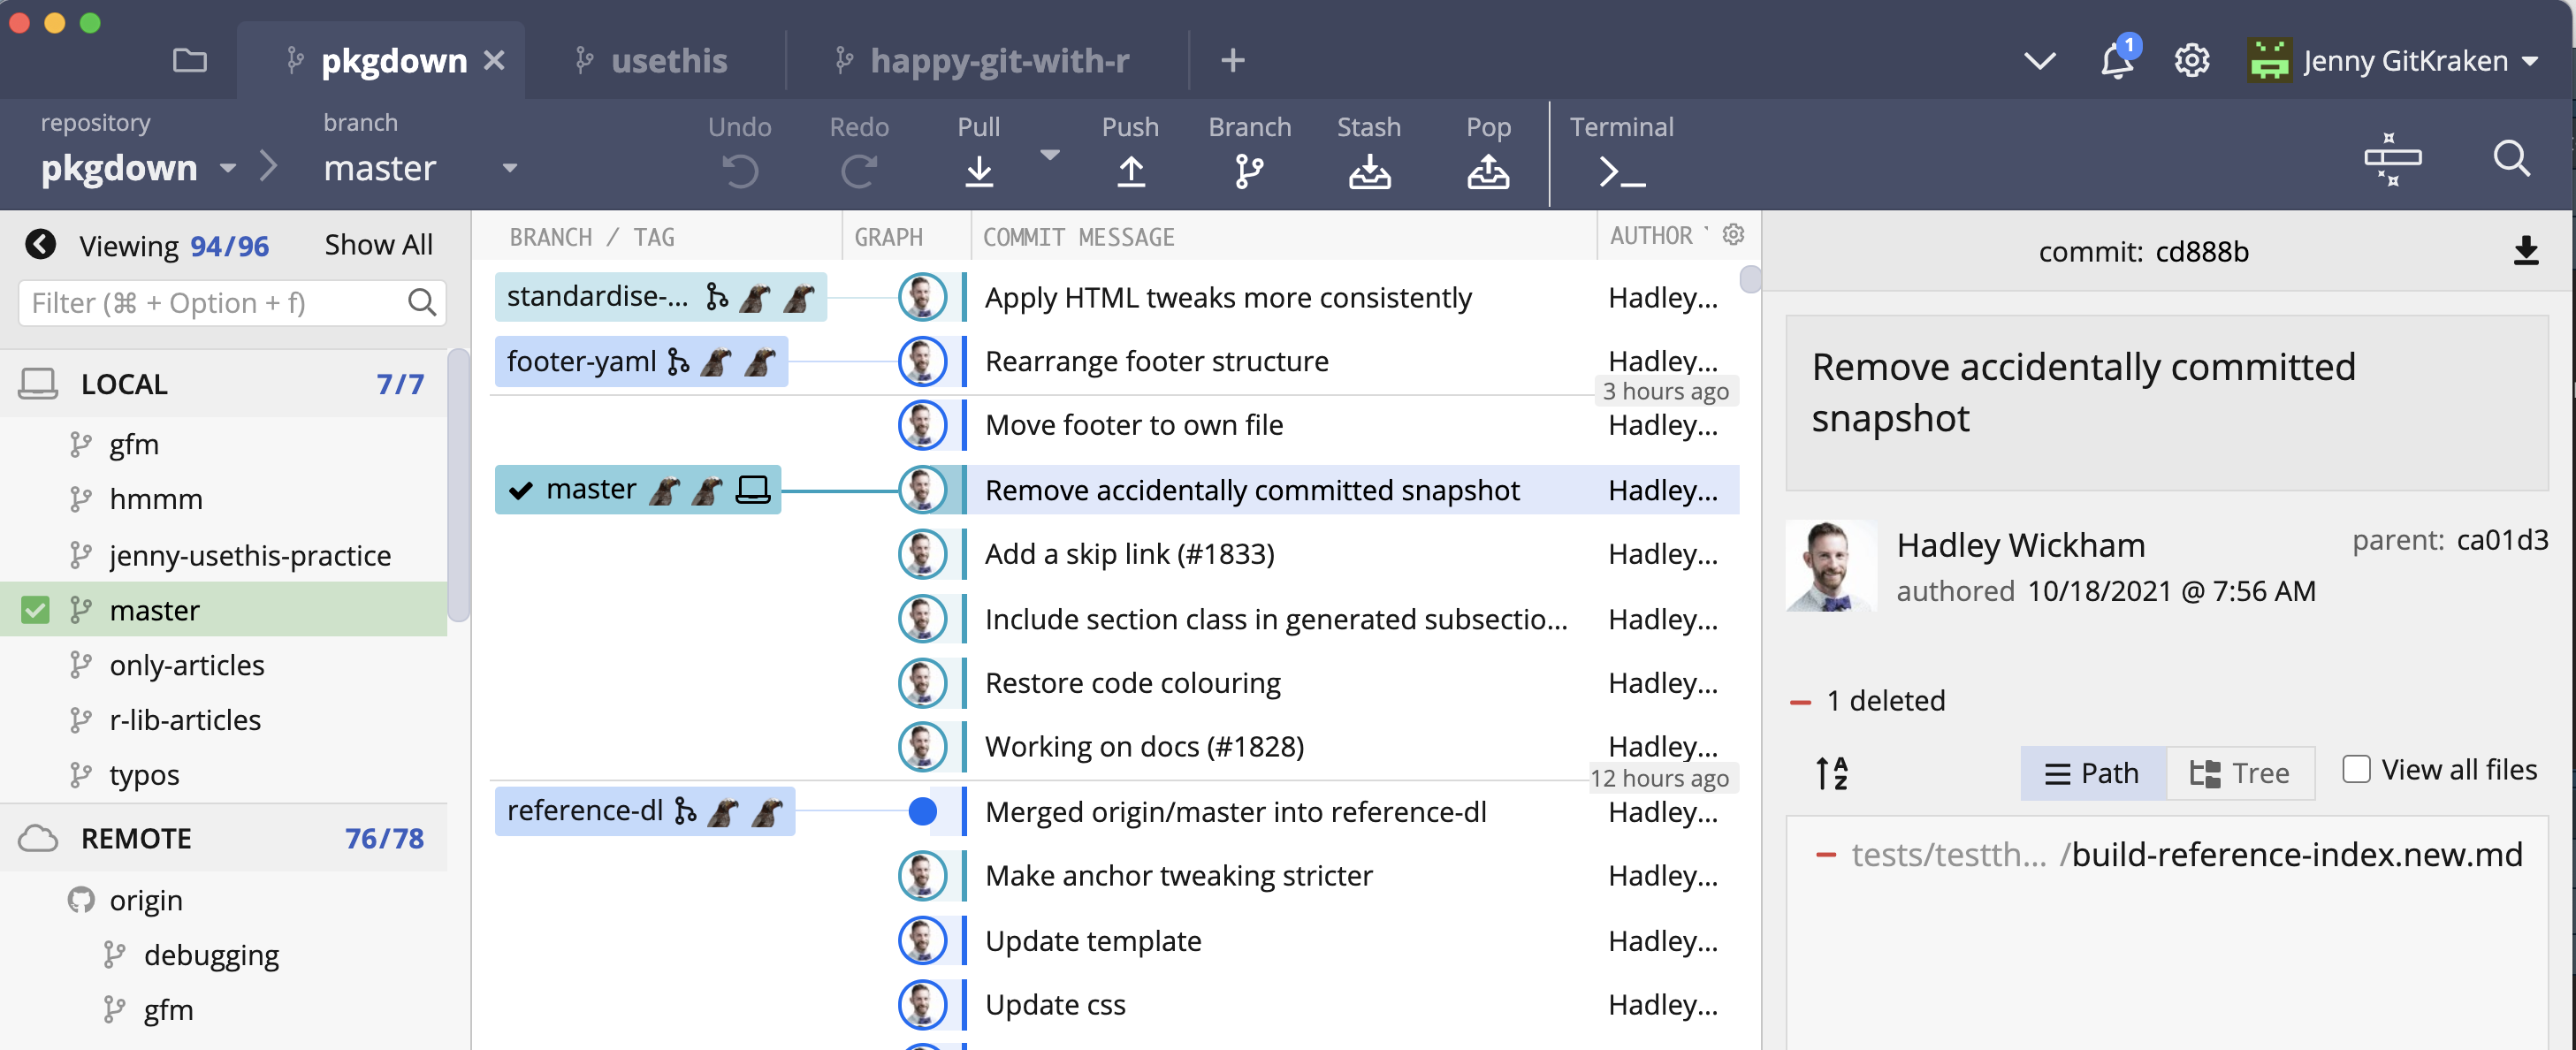
\includegraphics[width=1\linewidth]{img/gitkraken-pkgdown-screenshot} \end{center}

In contrast, here's a shell session where I've used command line Git to access some of the same information.

\begin{Shaded}
\begin{Highlighting}[]
\NormalTok{jenny@jennys{-}MacBook{-}Pro pkgdown \% git log {-}{-}oneline {-}n 10}
\NormalTok{cd888bed (HEAD {-}\textgreater{} master, upstream/master, upstream/HEAD, r{-}lib/master, r{-}lib/HEAD) Remove accidentally committed snapshot}
\NormalTok{ca01d386 Add a skip link (\#1833)}
\NormalTok{1f07a145 Include section class in generated subsection divs}
\NormalTok{26e1dcf2 Restore code colouring}
\NormalTok{77503979 Working on docs (\#1828)}
\NormalTok{3c805e1a Make anchor tweaking stricter}
\NormalTok{a6ae3ca4 use\_tidy\_description()}
\NormalTok{d43260fb Tweak authors order}
\NormalTok{41c855df Tweak details styling}
\NormalTok{7d3c484c Anchor \& news tweaks (\#1830)}
\end{Highlighting}
\end{Shaded}

Which do you prefer?

\section{No one is giving out Git Nerd merit badges}\label{no-one-is-giving-out-git-nerd-merit-badges}

Work with Git in whatever way makes you most effective.
Feel free to revisit your approach over time or to use different approaches for different tasks or in different settings.
No one can tell whether you use the command line or a GUI when they look at your Git history or your GitHub repo.

I sometimes encounter people who feel it's ``better'' to use command line Git, but for very ill-defined reasons.
These people may feel like they \emph{should} work in the shell, even if it leads to Git-avoidance, frequent mistakes, or limiting themselves to a small set of \textasciitilde3 Git commands.
This is counterproductive.

I had two false starts with Git, where I failed to get proficient enough, quickly enough to truly incorporate version control into my daily work.
I found a visual Git client invaluable.
It made me willing to use Git multiple times per day, for a sustained period of time.
This helped me build the mental model necessary for more advanced Git operations like rebasing, cherry-picking, and resetting.

If your Git life happens on your own computer, there is no reason to deny yourself a GUI if that's what you like.
If you prefer working in the shell or if you frequently log into a remote server, then it makes sense to prioritize building Git skills at the command line.
Do whatever works for you, but don't do anything for the sake of purity or heroism.

\section{Recommended Git clients}\label{recommended-git-clients}

\begin{itemize}
\item
  \href{https://www.gitkraken.com}{GitKraken} is a free, powerful Git(Hub) client that is my current favorite. It's especially exciting because it works on Windows, macOS, and Linux. This is great news, especially for long-suffering Linux users who previously had very few options. I used the free for version for years, which works great, but now I happily pay money for the pro version.
\item
  \href{https://www.sourcetreeapp.com}{SourceTree} is another free client that I used to highly recommend. It was my first beloved Git client, but I eventually had to give it up, due to long-standing bugs / deficiencies that seemed like they would never be fixed (\href{http://openradar.appspot.com/radar?id=1387401}{macOS bug re: leaking file handles}, no ability to control font size). GitKraken feels much more actively developed and has completely supplanted SourceTree for me.
\item
  GitHub offers a free Git(Hub) client, \href{https://desktop.github.com/}{GitHub Desktop}, for Windows and macOS. Although we previously discouraged its use, GitHub's client has since gotten a thorough makeover that eliminates several of our concerns, so we're cautiously optimistic. GitHub Desktop is aimed at beginners who want the most useful features of Git front and center. The flipside is that it may not support some of the more advanced workflows exposed by the clients above and, consequently, may not develop your mental model of Git as thoroughly.
\item
  Browse \href{http://git-scm.com/downloads/guis}{even more Git(Hub) clients}.
\end{itemize}

\part{Connect Git, GitHub, RStudio}\label{part-connect-git-github-rstudio}

\chapter*{Can you hear me now?}\label{connect-intro}
\addcontentsline{toc}{chapter}{Can you hear me now?}

The next few chapters walk through some basic operations to confirm you have installed the necessary software and that the necessary connections are being made, between tools on your computer and between your computer and GitHub.

This has a lot of overlap with some basic workflows we revisit later, but the second time around (or in a live workshop), we'll spend more time explaining what's happening and why.

Unfortunately, we have to front-load a rather fiddly task, which is to decide whether to communicate with GitHub via HTTPS or SSH and setup some credentials accordingly.
In \hyperref[https-pat]{Personal access token for HTTPS} we discuss how to choose between HTTPS and SSH and then walk through obtaining a personal access token, which is used with HTTPS.
Or, alternatively, we will help you \hyperref[ssh-keys]{Set up keys for SSH}.

Once we have our credentials sorted out, in \hyperref[push-pull-github]{Connect to GitHub}, we use Git in the shell to make sure you can clone a repo from GitHub and establish two-way communications, i.e.~pull and push.

In \hyperref[rstudio-git-github]{Connect RStudio to Git and GitHub} we confirm that RStudio can work with your Git installation to perform local operations and communicate with GitHub.

Hopefully you won't need it, but this part concludes with two troubleshooting chapters: \hyperref[rstudio-see-git]{Detect Git from RStudio} and \hyperref[troubleshooting]{RStudio, Git, GitHub Hell}.

\chapter{Personal access token for HTTPS}\label{https-pat}

When we interact with a remote Git server, such as GitHub, we have to include credentials in the request.
This proves we are a specific GitHub user, who's allowed to do whatever we're asking to do.

Git can communicate with a remote server using one of two protocols, HTTPS or SSH, and the different protocols use different credentials.

Here we describe the credential setup for the HTTPS protocol, which is what we recommend if you have no burning reason to pick SSH.
With HTTPS, we will use a \textbf{personal access token (PAT)}.
Head over to chapter \ref{ssh-keys} if you really want to set up SSH keys.

Let it be known that the password that you use to login to GitHub's website is NOT an acceptable credential when talking to GitHub as a Git server.
This was possible in the past (and may yet be true for other Git servers), but those days are over at GitHub.
You can learn more in their blog post \href{https://github.blog/2020-12-15-token-authentication-requirements-for-git-operations/}{Token authentication requirements for Git operations}.

Here's the error you'll see if you try to do that now:

\begin{Shaded}
\begin{Highlighting}[]
\NormalTok{remote: Support for password authentication was removed on August 13, 2021. Please use a personal access token instead.}
\NormalTok{remote: Please see https://github.blog/2020{-}12{-}15{-}token{-}authentication{-}requirements{-}for{-}git{-}operations/ for more information.}
\NormalTok{fatal: Authentication failed for \textquotesingle{}https://github.com/OWNER/REPO.git/\textquotesingle{}}
\end{Highlighting}
\end{Shaded}

The recommendation to use a personal access token (PAT) is exactly what we cover in this chapter.

\section{TL;DR}\label{tldr}

This is a very minimal account of getting and storing a PAT.
This might be all you need when you're first getting yourself set up.
You can always come back later and read other parts of this chapter.

Go to \url{https://github.com/settings/tokens} and click ``Generate token''.

Or, from R, do:

\begin{Shaded}
\begin{Highlighting}[]
\NormalTok{usethis}\SpecialCharTok{::}\FunctionTok{create\_github\_token}\NormalTok{()}
\end{Highlighting}
\end{Shaded}

Look over the scopes; I highly recommend selecting ``repo'', ``user'', and ``workflow''.
Recommended scopes will be pre-selected if you used \texttt{create\_github\_token()}.

Click ``Generate token''.

Copy the generated PAT to your clipboard.
Or leave that browser window open and available for a little while, so you can come back to copy the PAT.

Provide this PAT next time a Git operation asks for your password\footnote{Yes, it's confusing that you might be prompted for a password, but you should enter your PAT.
  GitHub no longer allows passwords in this context, but most basic Git tools still frame the authentication task with this language.}.

You could even get out ahead of this and store the PAT explicitly right now.
In R, call \texttt{gitcreds::gitcreds\_set()} to get a prompt where you can paste your PAT:

\begin{Shaded}
\begin{Highlighting}[]
\OperatorTok{\textgreater{}}\NormalTok{ gitcreds::gitcreds\_set}\KeywordTok{()}

\ExtensionTok{?}\NormalTok{ Enter password or token: ghp\_xxxxxxxxxxxxxxxxxxxxxxxxxxxxxxxxxxxx}
\ExtensionTok{{-}}\OperatorTok{\textgreater{}}\NormalTok{ Adding new credentials...}
\ExtensionTok{{-}}\OperatorTok{\textgreater{}}\NormalTok{ Removing credentials from cache...}
\ExtensionTok{{-}}\OperatorTok{\textgreater{}}\NormalTok{ Done.}
\end{Highlighting}
\end{Shaded}

You should be able to work with GitHub now, i.e.~push and pull.
If you're still doing your initial setup, now is a great time to move on to \hyperref[push-pull-github]{Connect to GitHub}.

Read on to learn more about:

\begin{itemize}
\tightlist
\item
  \hyperref[https-vs-ssh]{How to decide between the HTTPS and SSH protocols}
\item
  \hyperref[get-a-pat]{PAT scopes, names, and expiration}
\item
  \hyperref[store-pat]{PAT storage}
\item
  \hyperref[pat-troubleshooting]{Troubleshooting}
\end{itemize}

\section{HTTPS versus SSH}\label{https-vs-ssh}

I find HTTPS easier to get working quickly and \textbf{strongly recommend} it when you first start working with Git/GitHub.
HTTPS is what GitHub recommends, presumably for exactly the same reasons.
The ``ease of use'' argument in favor of HTTPS is especially true for Windows users.
I started with HTTPS, preferred SSH for a while, and have returned to HTTPS.
The main thing to know is that this is not an all-or-nothing decision and it's a relatively easy decision to revisit later.

Another advantage of HTTPS is that the PAT we'll set up for that can also be used with GitHub's REST API.
That might not mean anything to you (yet), but there are many R packages that call GitHub's API on your behalf (devtools+usethis, remotes, pak, gh, etc.).
Configuring your PAT kills two birds with one stone: this single credential can be used to authenticate to GitHub as a regular Git server and for its REST API.
If you authenticate via SSH for ``regular'' Git work, you will still have to set up a PAT for work that uses the REST API.

\begin{center}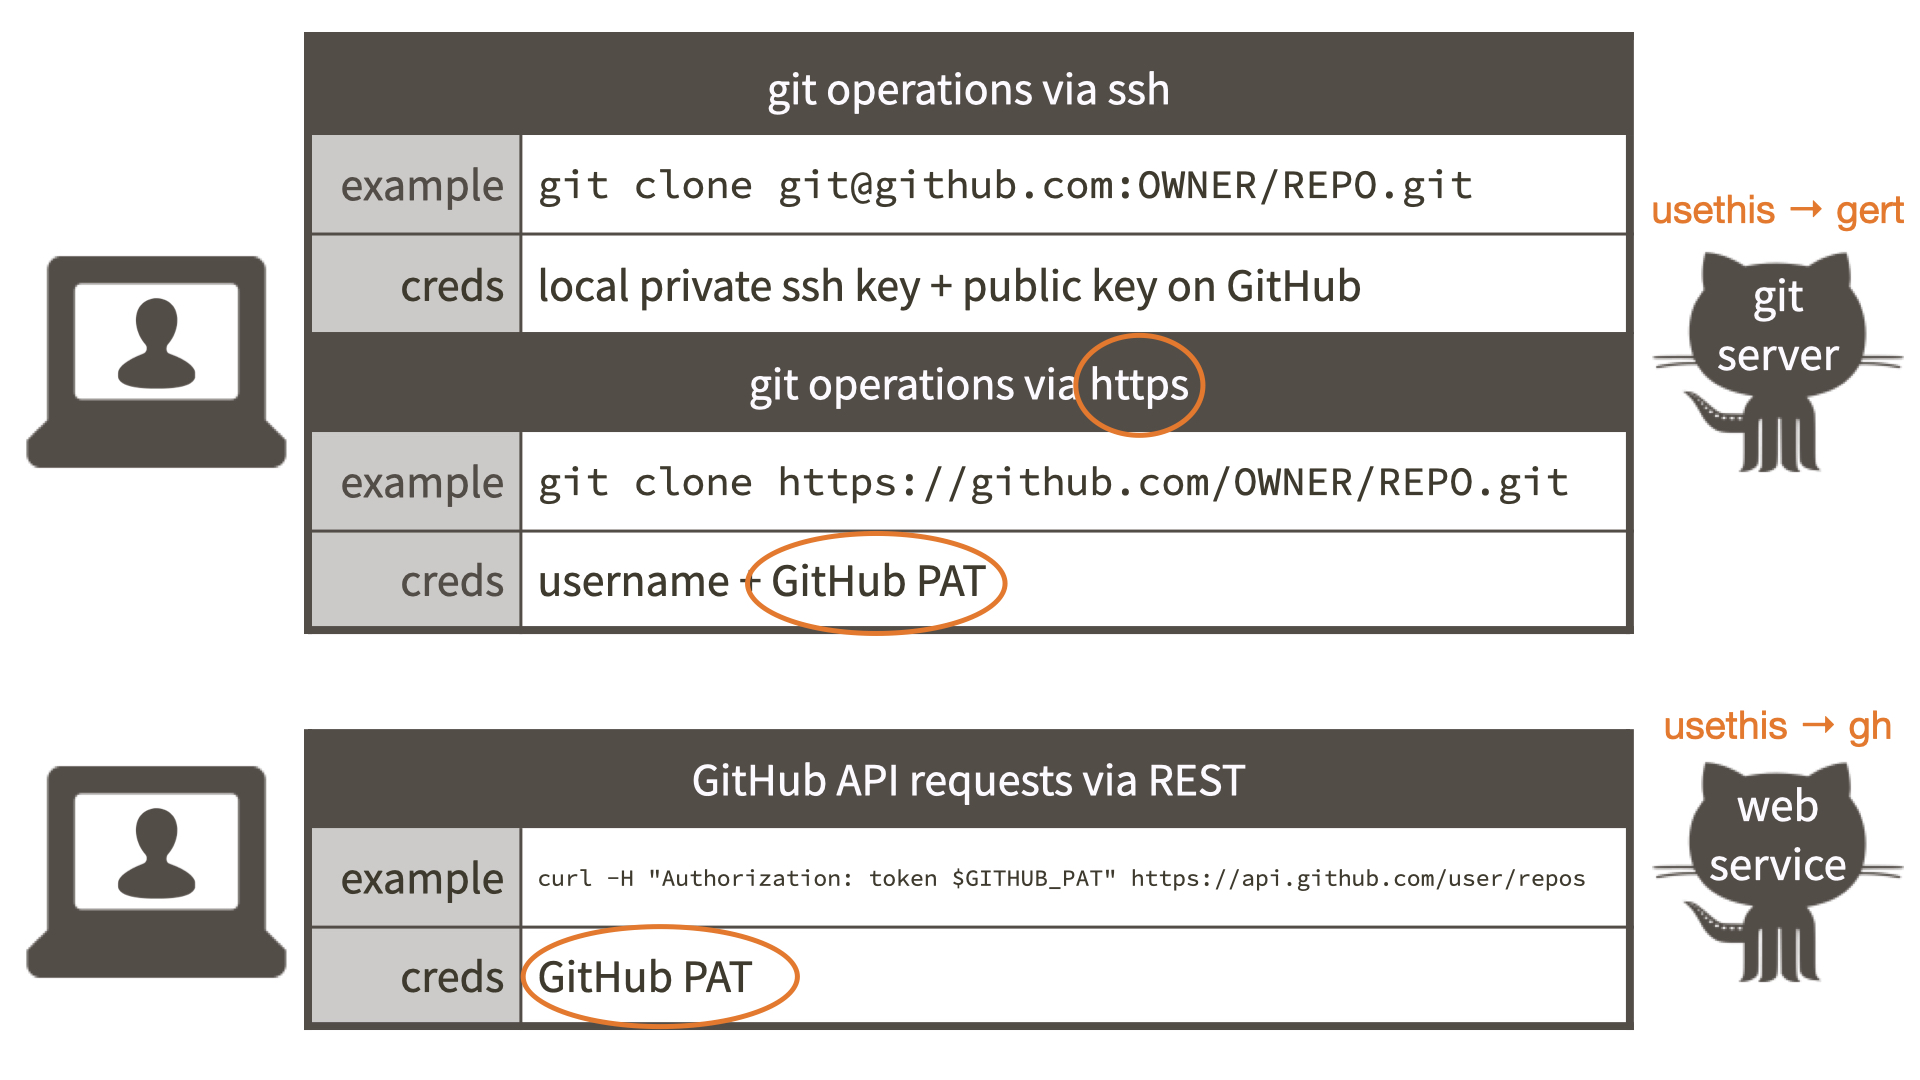
\includegraphics[width=0.8\linewidth]{img/pat-kills-both-birds} \end{center}

A properly configured PAT means all of this will ``just work'':

\begin{itemize}
\tightlist
\item
  Remote HTTPS operations via command line Git and, therefore, via RStudio
\item
  Remote HTTPS operations via the gert R package and, therefore, usethis
\item
  GitHub API operations via the gh R package and, therefore, usethis
\end{itemize}

\subsection{URL determines the protocol}\label{url-determines-protocol}

Even though I'm suggesting that you adopt HTTPS as a lifestyle, it's good to know that you actually have very granular control over the protocol.
It is determined by the URL used to access a remote repo.
Feel free to skip this section if you are new to Git (we mention some concepts and commands that won't make much sense 'til you've used Git a little).

HTTPS remote URLs look like \texttt{https://github.com/\textless{}OWNER\textgreater{}/\textless{}REPO\textgreater{}.git}.\\
SSH remote URLs look like \texttt{git@github.com:\textless{}OWNER\textgreater{}/\textless{}REPO\textgreater{}.git}.

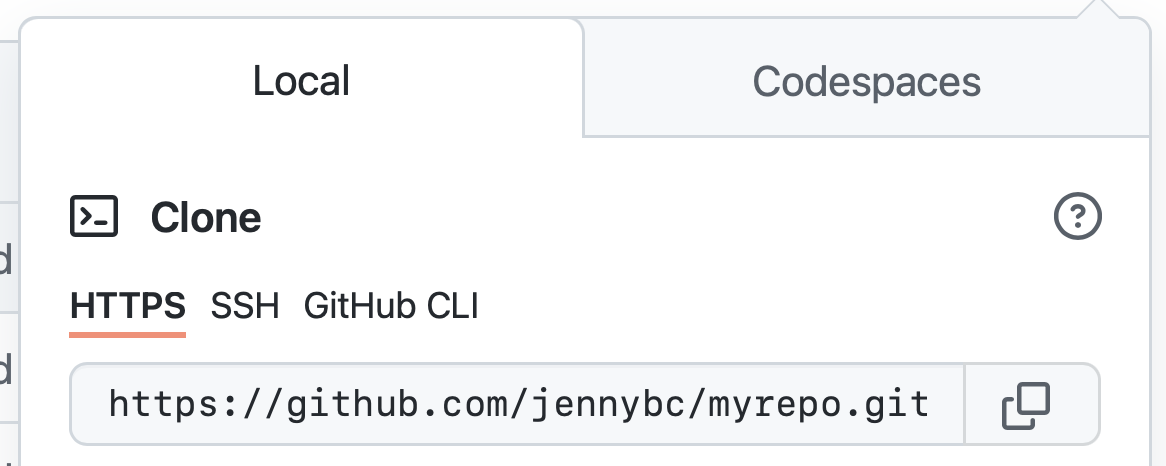
\includegraphics[width=0.49\linewidth,height=0.49\textheight]{img/github-https-url} 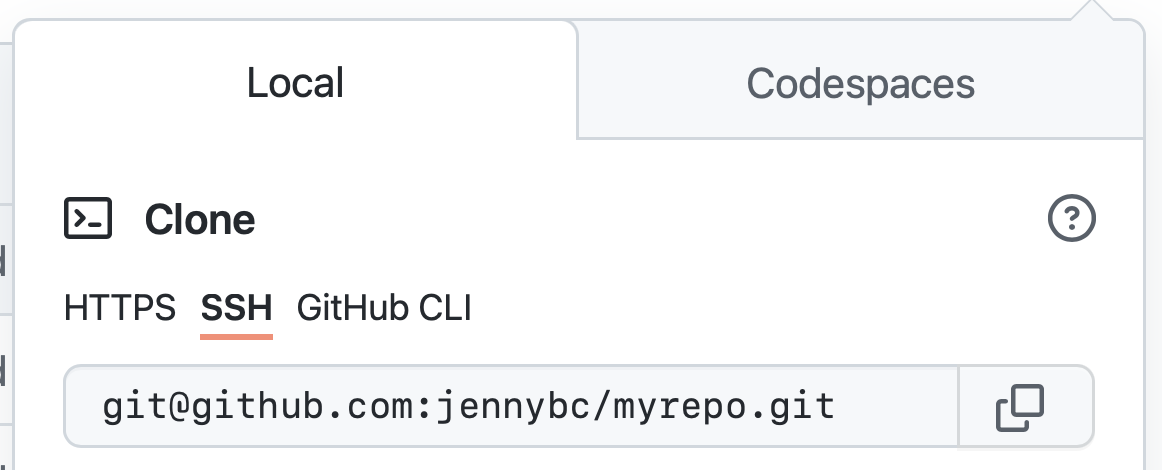
\includegraphics[width=0.49\linewidth,height=0.49\textheight]{img/github-ssh-url}

When you execute a command such as \texttt{git\ push\ origin\ my-cool-feature-branch}, Git looks up the URL you've stored for the \texttt{origin} remote and uses the protocol implicit in the URL's format.
The protocol is a game time decision.

This implies that:

\begin{itemize}
\tightlist
\item
  It's fine to use HTTPS for one remote in a repo and SSH for another.\\
\item
  It's fine to use HTTPS in one repo and SSH in another.\\
\item
  It's fine to interact with a GitHub repo via HTTPS from one computer and via SSH from another.\\
\item
  It's fine to adopt HTTPS for new work, even if some of your pre-existing repos use SSH.
\end{itemize}

You just have to be aware that mixed use of HTTPS and SSH means you'll have to configure both sorts of credentials.

Changing a specific remote from HTTPS to SSH (and back again) is a straightforward operation with \texttt{git\ remote\ set-url\ REMOTE\_NAME\ DESIRED\_URL}:

\begin{Shaded}
\begin{Highlighting}[]
\NormalTok{\textasciitilde{}/rrr/happy{-}git{-}with{-}r \% git remote {-}v}
\NormalTok{origin  https://github.com/jennybc/happy{-}git{-}with{-}r.git (fetch)}
\NormalTok{origin  https://github.com/jennybc/happy{-}git{-}with{-}r.git (push)}

\NormalTok{\textasciitilde{}/rrr/happy{-}git{-}with{-}r \% git remote set{-}url origin git@github.com:jennybc/happy{-}git{-}with{-}r.git}

\NormalTok{\textasciitilde{}/rrr/happy{-}git{-}with{-}r \% git remote {-}v}
\NormalTok{origin  git@github.com:jennybc/happy{-}git{-}with{-}r.git (fetch)}
\NormalTok{origin  git@github.com:jennybc/happy{-}git{-}with{-}r.git (push)}

\NormalTok{\textasciitilde{}/rrr/happy{-}git{-}with{-}r \% git remote set{-}url origin https://github.com/jennybc/happy{-}git{-}with{-}r.git}
\end{Highlighting}
\end{Shaded}

We can do the same from R using functions in usethis:

\begin{Shaded}
\begin{Highlighting}[]
\NormalTok{usethis}\SpecialCharTok{::}\FunctionTok{git\_remotes}\NormalTok{()}
\CommentTok{\#\textgreater{} $origin}
\CommentTok{\#\textgreater{} [1] "https://github.com/jennybc/happy{-}git{-}with{-}r.git"}

\NormalTok{usethis}\SpecialCharTok{::}\FunctionTok{use\_git\_remote}\NormalTok{(}
  \StringTok{"origin"}\NormalTok{,}
  \StringTok{"git@github.com:jennybc/happy{-}git{-}with{-}r.git"}\NormalTok{,}
  \AttributeTok{overwrite =} \ConstantTok{TRUE}
\NormalTok{)}

\NormalTok{usethis}\SpecialCharTok{::}\FunctionTok{git\_remotes}\NormalTok{()}
\CommentTok{\#\textgreater{} $origin}
\CommentTok{\#\textgreater{} [1] "git@github.com:jennybc/happy{-}git{-}with{-}r.git"}

\NormalTok{usethis}\SpecialCharTok{::}\FunctionTok{use\_git\_remote}\NormalTok{(}
  \StringTok{"origin"}\NormalTok{,}
  \StringTok{"https://github.com/jennybc/happy{-}git{-}with{-}r.git"}\NormalTok{,}
  \AttributeTok{overwrite =} \ConstantTok{TRUE}
\NormalTok{)}
\end{Highlighting}
\end{Shaded}

\section{Generate a personal access token (PAT)}\label{get-a-pat}

On github.com, assuming you're signed in, you can manage your personal access tokens from \url{https://github.com/settings/tokens}, also reachable via \emph{Settings \textgreater{} Developer settings \textgreater{} Personal access tokens}.
You could click on ``Generate new token'' here or, perhaps even better, you could call \texttt{usethis::create\_github\_token()} from R:

\begin{Shaded}
\begin{Highlighting}[]
\NormalTok{usethis}\SpecialCharTok{::}\FunctionTok{create\_github\_token}\NormalTok{()}
\end{Highlighting}
\end{Shaded}

The usethis approach takes you to a pre-filled form where we have pre-selected some recommended scopes, which you can look over and adjust before clicking ``Generate token''.
At the time of writing, the usethis-recommended scopes are ``repo'', ``user'', ``gist'', and ``workflow''.

\begin{center}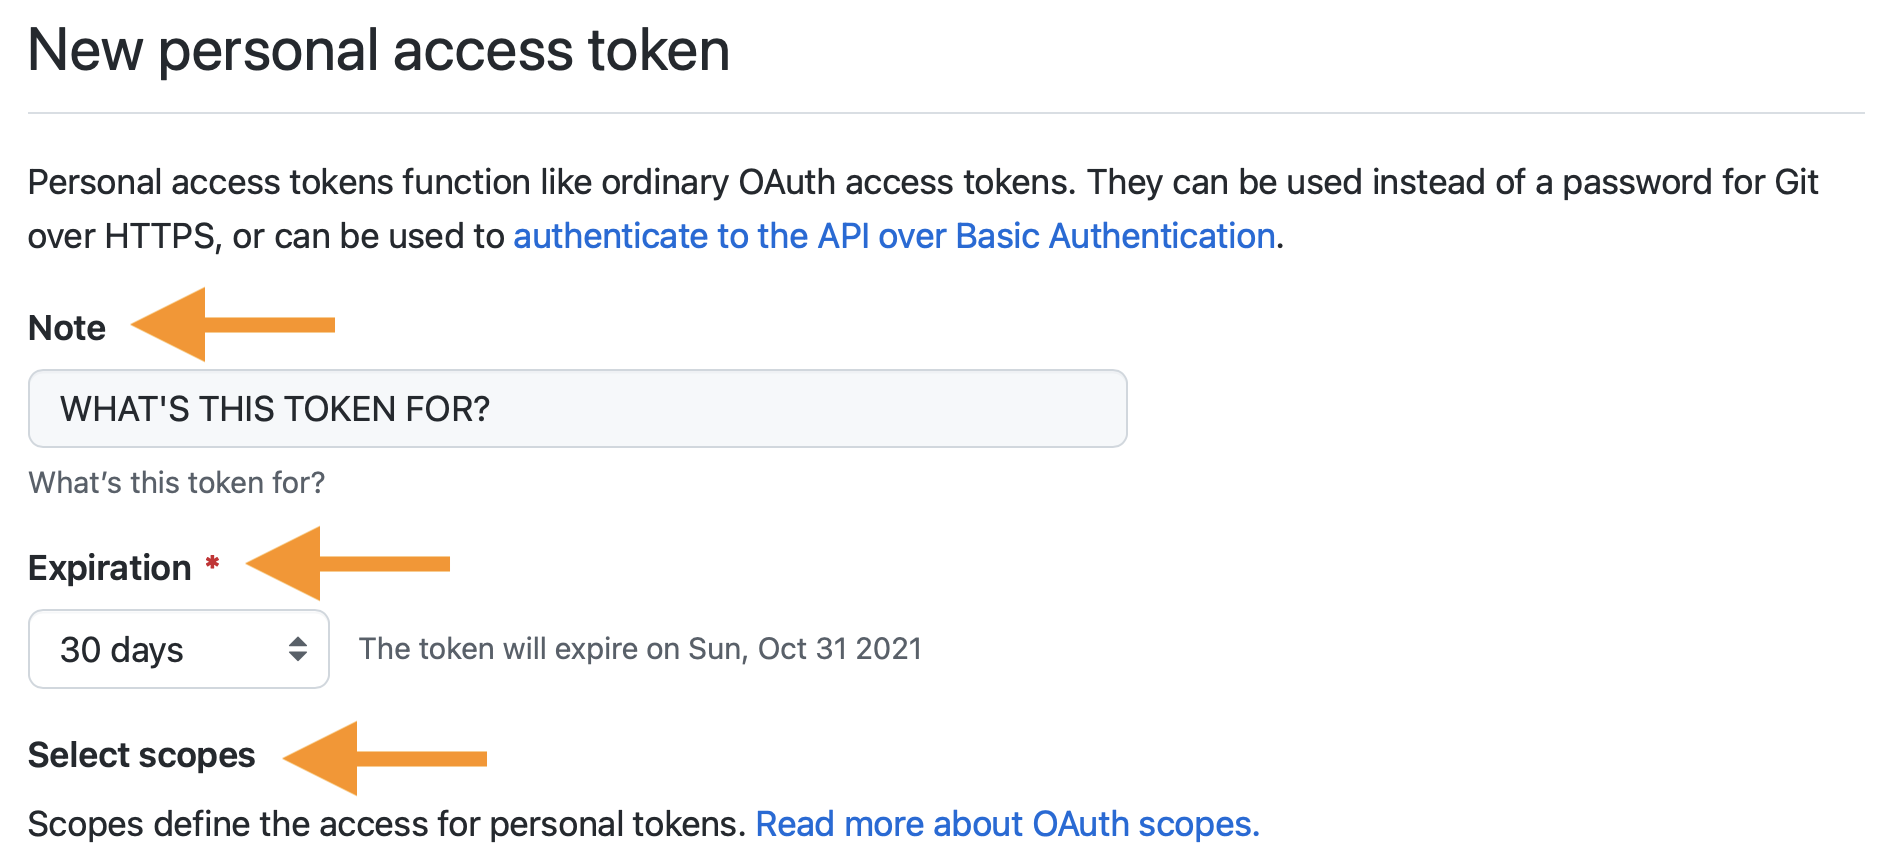
\includegraphics[width=1\linewidth]{img/new-personal-access-token-screenshot} \end{center}

It is a very good idea to describe the token's purpose in the \emph{Note} field, because one day you might have multiple PATs.
We recommend naming each token after its use case, such as the computer or project you are using it for, e.g.~``personal-macbook-air'' or ``vm-for-project-xyz''.
In the future, you will find yourself staring at this list of tokens, because inevitably you'll need to re-generate or delete one of them.
Make it easy to figure out which token you've come here to fiddle with.

GitHub encourages the use of perishable tokens, with a default \emph{Expiration} period of 30 days.
Unless you have a specific reason to fight this, I recommend accepting this default.
I assume that GitHub's security folks have good reasons for their recommendation.
But, of course, you can adjust the \emph{Expiration} behaviour as you see fit, including ``No expiration''.

Once you're happy with the token's \emph{Note}, \emph{Expiration}, and \emph{Scopes}, click ``Generate token''.

You won't be able to see this token again, so don't close or navigate away from this browser window until you store the PAT locally.
Copy the PAT to the clipboard, anticipating what we'll do next: trigger a prompt that lets us store the PAT in the Git credential store.

Treat this PAT like a password!
Do not ever hard-wire your PAT into your code!
A PAT should always be retrieved implicitly, for example, from the Git credential store.
We're about to help you store the PAT in a safe place, where command line Git, RStudio, and R packages can discover it.

If you use a password management app, such as 1Password or LastPass (highly recommended!), you might want to also add this PAT (and its \emph{Note}) to the entry for GitHub, where you're already storing your username and password.
Storing your PAT in the Git credential store is a semi-persistent convenience, sort of like a browser cache or ``remember me'' on a website\footnote{Haha! We all know how well ``remember me'' works.} and it's conceivable you will need to re-enter your PAT in the future.
You could decide to embrace the impermanence of your PAT and, if it somehow goes missing, you'll just \hyperref[regenerate-pat]{re-generate the PAT and re-store it}.
If you accept the default 30-day expiration period, this is a workflow you'll be using often anyway.
But if you create long-lasting tokens or want to feel free to play around with the functions for setting or clearing your Git credentials, it can be handy to have your own record of your PAT in a secure place, like 1Password or LastPass.

\section{Store your PAT}\label{store-pat}

At this point, I assume you've generated a PAT and have it available, in one or both of these ways:

\begin{itemize}
\tightlist
\item
  In a secure, long-term system for storing secrets, like 1Password or LastPass
\item
  For the next few minutes, in a browser window or on the clipboard
\end{itemize}

There are a couple ways to get your PAT into the Git credential store:

\begin{itemize}
\tightlist
\item
  Call an R function to explicitly store (or update) your credentials.
\item
  Do something in command line Git or RStudio that triggers a credential
  challenge.
\end{itemize}

\subsection{Call an R function to store your credentials}\label{call-an-r-function-to-store-your-credentials}

There are two R packages for accessing the Git credential store:

\begin{itemize}
\tightlist
\item
  \href{https://r-lib.github.io/gitcreds/}{gitcreds}
\item
  \href{https://docs.ropensci.org/credentials/}{credentials}
\end{itemize}

It is likely that these packages will eventually combine into one and, even now, they are largely interoperable.
You don't need to follow the instructions for both packages -- pick one!

\subsubsection{gitcreds package}\label{gitcreds-package}

If you don't have gitcreds installed, install via \texttt{install.packages("gitcreds")}.
If you've installed usethis, you will already have gitcreds, because usethis uses gh and gh uses gitcreds.

Call \texttt{gitcreds::gitcreds\_set()}.
If you don't have a PAT stored already, it will prompt you to enter your PAT. Paste!

\begin{Shaded}
\begin{Highlighting}[]
\OperatorTok{\textgreater{}}\NormalTok{ gitcreds::gitcreds\_set}\KeywordTok{()}

\ExtensionTok{?}\NormalTok{ Enter password or token: ghp\_xxxxxxxxxxxxxxxxxxxxxxxxxxxxxxxxxxxx}
\ExtensionTok{{-}}\OperatorTok{\textgreater{}}\NormalTok{ Adding new credentials...}
\ExtensionTok{{-}}\OperatorTok{\textgreater{}}\NormalTok{ Removing credentials from cache...}
\ExtensionTok{{-}}\OperatorTok{\textgreater{}}\NormalTok{ Done.}
\end{Highlighting}
\end{Shaded}

If you already have a stored credential, \texttt{gitcreds::gitcreds\_set()} reveals this and will even let you inspect it.
This helps you decide whether to keep the existing credential or replace it.
When in doubt, embrace a new, known-to-be-good credential over an old one, of dubious origins.

\begin{Shaded}
\begin{Highlighting}[]
\OperatorTok{\textgreater{}}\NormalTok{ gitcreds::gitcreds\_set}\KeywordTok{()}

\ExtensionTok{{-}}\OperatorTok{\textgreater{}}\NormalTok{ Your current credentials for }\StringTok{\textquotesingle{}https://github.com\textquotesingle{}}\NormalTok{:}

  \ExtensionTok{protocol:}\NormalTok{ https}
  \ExtensionTok{host}\NormalTok{    : github.com}
  \ExtensionTok{username:}\NormalTok{ PersonalAccessToken}
  \ExtensionTok{password:} \OperatorTok{\textless{}}\NormalTok{{-}{-} hidden }\AttributeTok{{-}{-}}\OperatorTok{\textgreater{}}

\ExtensionTok{{-}}\OperatorTok{\textgreater{}}\NormalTok{ What would you like to do}\PreprocessorTok{?} 

\ExtensionTok{1:}\NormalTok{ Keep these credentials}
\ExtensionTok{2:}\NormalTok{ Replace these credentials}
\ExtensionTok{3:}\NormalTok{ See the password / token}

\ExtensionTok{Selection:}\NormalTok{ 2}

\ExtensionTok{{-}}\OperatorTok{\textgreater{}}\NormalTok{ Removing current credentials...}

\ExtensionTok{?}\NormalTok{ Enter new password or token: ghp\_xxxxxxxxxxxxxxxxxxxxxxxxxxxxxxxxxxxx}
\ExtensionTok{{-}}\OperatorTok{\textgreater{}}\NormalTok{ Adding new credentials...}
\ExtensionTok{{-}}\OperatorTok{\textgreater{}}\NormalTok{ Removing credentials from cache...}
\ExtensionTok{{-}}\OperatorTok{\textgreater{}}\NormalTok{ Done.}
\end{Highlighting}
\end{Shaded}

You can check that you've stored a credential with \texttt{gitcreds\_get()}:

\begin{Shaded}
\begin{Highlighting}[]
\FunctionTok{gitcreds\_get}\NormalTok{()}
\CommentTok{\#\textgreater{} \textless{}gitcreds\textgreater{}}
\CommentTok{\#\textgreater{}   protocol: https}
\CommentTok{\#\textgreater{}   host    : github.com}
\CommentTok{\#\textgreater{}   username: PersonalAccessToken}
\CommentTok{\#\textgreater{}   password: \textless{}{-}{-} hidden {-}{-}\textgreater{}}
\end{Highlighting}
\end{Shaded}

Other functions that can help you feel confident about your PAT setup include:

\begin{Shaded}
\begin{Highlighting}[]
\NormalTok{usethis}\SpecialCharTok{::}\FunctionTok{gh\_token\_help}\NormalTok{()}

\NormalTok{usethis}\SpecialCharTok{::}\FunctionTok{git\_sitrep}\NormalTok{()}

\NormalTok{gh}\SpecialCharTok{::}\FunctionTok{gh\_whoami}\NormalTok{()}
\end{Highlighting}
\end{Shaded}

\subsubsection{credentials package}\label{credentials-package}

If you don't have credentials installed, install via \texttt{install.packages("credentials")}.
If you've installed usethis, you will already have credentials, because usethis uses gert and gert uses credentials.

Call \texttt{set\_github\_pat()}.
If you don't have a PAT stored already, it will prompt you to enter your PAT. Paste!

\begin{Shaded}
\begin{Highlighting}[]
\NormalTok{credentials}\SpecialCharTok{::}\FunctionTok{set\_github\_pat}\NormalTok{()}
\end{Highlighting}
\end{Shaded}

If successful, your initial (and subsequent) calls will look like this:

\begin{Shaded}
\begin{Highlighting}[]
\NormalTok{credentials}\SpecialCharTok{::}\FunctionTok{set\_github\_pat}\NormalTok{()}
\CommentTok{\#\textgreater{} If prompted for GitHub credentials, enter your PAT in the password field}
\CommentTok{\#\textgreater{} Using GITHUB\_PAT from Jennifer (Jenny) Bryan (credential helper: osxkeychain)}
\end{Highlighting}
\end{Shaded}

Other functions that can help you feel confident about your PAT setup include:

\begin{Shaded}
\begin{Highlighting}[]
\NormalTok{usethis}\SpecialCharTok{::}\FunctionTok{gh\_token\_help}\NormalTok{()}

\NormalTok{usethis}\SpecialCharTok{::}\FunctionTok{git\_sitrep}\NormalTok{()}

\NormalTok{gh}\SpecialCharTok{::}\FunctionTok{gh\_whoami}\NormalTok{()}
\end{Highlighting}
\end{Shaded}

\subsection{Store credentials through organic Git use}\label{store-credentials-through-organic-git-use}

\emph{Before gitcreds and credentials existed (see above), we had to orchestrate a credential challenge by setting up (and then tearing down) a toy repo.
That still occurs naturally in the guided exercise in \hyperref[push-pull-github]{Connect to GitHub}.
But I strongly recommend managing your PAT more directly and explicitly with
\texttt{gitcreds::gitcreds\_set()} and related functions in gitcreds.}

\section{HTTPS PAT problems and solutions}\label{pat-troubleshooting}

This section is for people who need to know even more about PAT management, because they're in a nonstandard situation or troubleshooting.

\subsection{Valid PAT gets stored, but later told the PAT is invalid}\label{valid-pat-gets-stored-but-later-told-the-pat-is-invalid}

Let's say you generate a fresh PAT and successfully store it as described above.
Maybe you even use it successfully.
But later, you're told your PAT is invalid!
How can this be?

Here are some likely explanations:

\begin{enumerate}
\def\labelenumi{\arabic{enumi}.}
\tightlist
\item
  Your PAT truly is invalid. By default, PATs have an expiration date now. One
  day you really will wake up and find the PAT has gone bad overnight and you
  need to re-generate and re-store it.
\item
  You have an invalid PAT stored \emph{somewhere else}, that you've forgotten about,
  probably in \texttt{.Renviron}. This old, invalid PAT is preventing R packages from
  even discovering your new, valid PAT.
\end{enumerate}

\subsubsection{PAT has expired}\label{regenerate-pat}

You are going to be re-generating and re-storing your PAT on a schedule dictated by its expiration period.
By default, once per month.

When the PAT expires, return to \url{https://github.com/settings/tokens} and click on its \emph{Note}.
(You do label your tokens nicely by use case, right? Right?)
At this point, you can optionally adjust scopes and then click ``Regenerate token''.
You can optionally modify its \emph{Expiration} and then click ``Regenerate token'' (again).
As before, copy the PAT to the clipboard, call \texttt{gitcreds::gitcreds\_set()}, and paste!

Hopefully it's becoming clear why each token's \emph{Note} is so important.
The actual token may be changing, e.g., once a month, but its use case (and scopes) are much more persistent and stable.

\subsubsection{\texorpdfstring{Old \texttt{GITHUB\_PAT} in \texttt{.Renviron}}{Old GITHUB\_PAT in .Renviron}}\label{old-github_pat-in-.renviron}

These usethis functions will diagnose this problem:

\begin{Shaded}
\begin{Highlighting}[]
\NormalTok{usethis}\SpecialCharTok{::}\FunctionTok{gh\_token\_help}\NormalTok{()}

\NormalTok{usethis}\SpecialCharTok{::}\FunctionTok{git\_sitrep}\NormalTok{()}
\end{Highlighting}
\end{Shaded}

In the past, it was common to store a PAT as the \texttt{GITHUB\_PAT} environment variable in \texttt{.Renviron}.
But now, thanks to gitcreds and credentials, we can store and retrieve a PAT, from R, the same way as command line Git does.

If you have any doubt about your previous practices, open \texttt{.Renviron}, look for a line setting the \texttt{GITHUB\_PAT} environment variable, and delete it. \texttt{usethis::edit\_r\_environ()} can be helpful for getting \texttt{.Renviron} open for editing.
Don't forget to restart R for this change to take effect.

\subsection{PAT doesn't persist on macOS or Windows}\label{pat-doesnt-persist-on-macos-or-windows}

The credential helpers used by Git take advantage of official OS-provided credential stores, where possible, such as macOS Keychain and Windows Credential Manager.

If you're trying to follow the advice here and your PAT never persists, consider that you may need to update Git to get its more modern credential helpers.
This is absolutely an area of Git that has improved rapidly in recent years and the gitcreds and credentials package work best with recent versions of Git.
I have not needed to explicitly activate a credential helper on macOS or Windows with any recent version of Git.

Here's a command to reveal the current credential helper and what I see these days.

macOS

\begin{Shaded}
\begin{Highlighting}[]
\NormalTok{$ git config {-}{-}show{-}origin {-}{-}get credential.helper}
\NormalTok{file:/Users/jenny/.gitconfig    osxkeychain}
\end{Highlighting}
\end{Shaded}

Windows

\begin{Shaded}
\begin{Highlighting}[]
\NormalTok{$ git config {-}{-}show{-}origin {-}{-}get credential.helper}
\NormalTok{file:C:/Program Files/Git/mingw64/etc/gitconfig manager}
\end{Highlighting}
\end{Shaded}

If you want to know how more about how gitcreds and credentials are managing your PAT, learn about \href{https://git-scm.com/docs/git-credential}{\texttt{git\ credential\ \textless{}fill\textbar{}approve\textbar{}reject\textgreater{}}}.
For keeners, that documentation gives you the gory details on how credentials are stored and retrieved:

\begin{quote}
Git has an internal interface for storing and retrieving credentials from system-specific helpers, as well as prompting the user for usernames and passwords. The \texttt{git-credential} command exposes this interface to scripts which may want to retrieve, store, or prompt for credentials in the same manner as Git.
\end{quote}

On Windows, your Git credentials are probably being stored via Credential Manager.

On macOS, your Git credentials are probably being stored in the Keychain.

If you really want to poke around directly to explore or clean out your GitHub credentials, launch Credential Manager (Windows) or Keychain Access (macOS) and search for ``github.com''.

\subsection{PAT doesn't persist on Linux}\label{pat-doesnt-persist-on-linux}

The credential helpers used by Git take advantage of official OS-provided
credential stores on macOS and Windows, but sadly there is no exact equivalent on Linux.

The easiest thing to do is to configure Git to ``cache'' your credentials (vs ``store''), which is more time-limited.
Then set the cache timeout to some suitably long period of time.
Here, we set the timeout to ten million seconds or around 16 weeks, enough for a semester.

\begin{Shaded}
\begin{Highlighting}[]
\NormalTok{git config {-}{-}global credential.helper \textquotesingle{}cache {-}{-}timeout=10000000\textquotesingle{}}
\end{Highlighting}
\end{Shaded}

This still may not make your PAT available to R packages.
In this case, you may need to use the older, less secure approach of storing your PAT in \texttt{.Renviron}.
\texttt{usethis::edit\_r\_environ()} opens that file for editing.

\begin{Shaded}
\begin{Highlighting}[]
\NormalTok{usethis}\SpecialCharTok{::}\FunctionTok{edit\_r\_environ}\NormalTok{()}
\end{Highlighting}
\end{Shaded}

Add a line like this, but substitute your PAT:

\begin{Shaded}
\begin{Highlighting}[]
\VariableTok{GITHUB\_PAT}\OperatorTok{=}\NormalTok{ghp\_xxxxxxxxxxxxxxxxxxxxxxxxxxxxxxxxxxxx}
\end{Highlighting}
\end{Shaded}

Make sure this file ends in a newline!
Lack of a newline can lead to silent failure to load startup files, which can be tricky to debug.
Take care that this file is not accidentally pushed to the cloud, e.g.~Google Drive or GitHub.

Restart R for changes in \texttt{.Renviron} to take effect.

\chapter{Set up keys for SSH}\label{ssh-keys}

When we interact with a remote Git server, such as GitHub, we have to include credentials in the request.
This proves we are a specific GitHub user, who's allowed to do whatever we're asking to do.

Git can communicate with a remote server using one of two protocols, HTTPS or SSH, and the different protocols use different credentials.

Here we describe the credential setup for the SSH protocol.
If you're not sure whether to use HTTPS or SSH, please read \hyperref[https-vs-ssh]{HTTPS versus SSH}.
From now on, we assume you've made an intentional choice to set up SSH keys.

\section{SSH keys}\label{ssh-keys-1}

SSH keys provide a more secure way of logging into a server than using a password alone. While a password can eventually be cracked with a brute force attack, SSH keys are nearly impossible to decipher by brute force alone. Generating a key pair provides you with two long strings of characters: a public and a private key. You can place the public key on any server (like GitHub!), and then unlock it by connecting to it with a client that already has the private key (your computer!). When the two match up, the system unlocks without the need for a password. You can increase security even more by protecting the private key with a passphrase.

Adapted from instructions provided by \href{https://help.github.com/categories/ssh/}{GitHub} and \href{https://www.digitalocean.com/community/tutorials/how-to-set-up-ssh-keys--2}{Digital Ocean}.

\section{SSH outline and advice}\label{ssh-outline-and-advice}

High level overview of what must happen:

\begin{itemize}
\tightlist
\item
  Create a public-private SSH key pair. Literally, 2 special files, in a special place. Optionally, encrypt the private key with a passphrase (best practice).
\item
  Add the private key to your ssh-agent. If you protected it with a passphrase, you may have additional configuration.
\item
  Add your public key to your GitHub profile.
\end{itemize}

Advice:

\begin{itemize}
\tightlist
\item
  If you are new to programming and the shell, you'll probably find HTTPS easier at first (chapter \ref{https-pat}). You can always switch to SSH later. You can use one method from computer A and the other from computer B.
\item
  You should swap out your SSH keys periodically. Something like once a year.
\item
  It's best practice to protect your private key with a passphrase. This can make setup and usage harder, so if you're not up for that (yet), either don't use a passphrase or seriously consider using HTTPS instead.
\item
  Don't do weird gymnastics in order to have only one key pair, re-used over multiple computers. You should probably have one key per computer (I do this). Some people even have one key per computer, per service (I do not do this).
\item
  It is normal to associate multiple public keys with your GitHub account. For example, one public key for each computer you connect with.
\end{itemize}

\section{Do you already have keys?}\label{do-you-already-have-keys}

You can check this from RStudio or from the shell.

Global advice: if you do have existing keys, but have no clue where they came from or why you created them, you should seriously consider creating a new SSH key pair. It's up to you to figure out whether/how to delete the old ones. But don't let that keep you from creating new keys and moving forward.

\subsection{From RStudio}\label{from-rstudio}

Go to \emph{Tools \textgreater{} Global Options\ldots\textgreater{} Git/SVN}. If you see something like \texttt{\textasciitilde{}/.ssh/id\_rsa} in the SSH RSA Key box, you definitely have existing keys.

Caveat: RStudio only looks for a key pair named \texttt{id\_rsa} and \texttt{id\_rsa.pub}.
This makes sense, because historically that has been the most common.

However, these days both GitHub and GitLab are encouraging users to generate SSH keys with the Ed25519 algorithm, which results in a key pair named \texttt{id\_ed25519} and \texttt{id\_ed25519.pub}.
At the time of writing, RStudio will not display such a key pair, which can be confusing.
Therefore, it's probably a good idea to also check for existing keys in the shell.

\subsection{From the shell}\label{from-the-shell}

Go to the shell (appendix \ref{shell}).

List existing keys:

\begin{Shaded}
\begin{Highlighting}[]
\NormalTok{ls {-}al \textasciitilde{}/.ssh/}
\end{Highlighting}
\end{Shaded}

If you are told \texttt{\textasciitilde{}/.ssh/} doesn't exist, you don't have SSH keys!

If you see a pair of files like \texttt{id\_rsa.pub} and \texttt{id\_rsa} or \texttt{id\_ed25519} and \texttt{id\_ed25519.pub}, you have a key pair already.
The typical pattern is \texttt{id\_FOO.pub} (the public key) and \texttt{id\_FOO} (the private key), where \texttt{FOO} reflects the key type.
If you're happy to stick with your existing keys, skip to the sections about adding a key to the ssh-agent and GitHub.

\section{Create an SSH key pair}\label{create-an-ssh-key-pair}

\subsection{Option 1: Set up from RStudio}\label{option-1-set-up-from-rstudio}

Go to \emph{Tools \textgreater{} Global Options\ldots\textgreater{} Git/SVN \textgreater{} Create RSA Key\ldots{}}.

RStudio prompts you for a passphrase. It is optional, but also a best practice. Configuring your system for smooth operation with a passphrase-protected key introduces more moving parts.
If you're completely new at all this, skip the passphrase (or use HTTPS!) and implement it next time, when you are more comfortable with system configuration.
I did not use a passphrase at first, but I do now, and record it in a password manager.

Click ``Create'' and RStudio will generate an SSH key pair, stored in the files \texttt{\textasciitilde{}/.ssh/id\_rsa} and \texttt{\textasciitilde{}/.ssh/id\_rsa.pub}.

Note that RStudio currently only generates RSA keys, whereas the standard recommendation by GitHub and GitLab is to use Ed25519 keys.
If you want to comply with that advice, generate your keys in the shell for now.

\subsection{Option 2: Set up from the shell}\label{option-2-set-up-from-the-shell}

Create the key pair like so, but substitute a comment that means something to you, especially if you'll have multiple SSH keys in your life.
Consider the email associated with your GitHub account or the name of your computer or some combination, e.g.~\texttt{your\_email@example.com} or \texttt{macbook-pro} or \texttt{jane-2020-macbook-pro}.

\begin{Shaded}
\begin{Highlighting}[]
\NormalTok{ssh{-}keygen {-}t ed25519 {-}C "DESCRIPTIVE{-}COMMENT"}
\end{Highlighting}
\end{Shaded}

If it appears that your system is too old to support the Ed25519 algorithm, do this instead:

\begin{Shaded}
\begin{Highlighting}[]
\NormalTok{ssh{-}keygen {-}t rsa {-}b 4096 {-}C "DESCRIPTIVE{-}COMMENT"}
\end{Highlighting}
\end{Shaded}

Accept the proposal to save the key in the default location.
Just press Enter here:

\begin{Shaded}
\begin{Highlighting}[]
\NormalTok{Enter file in which to save the key (/Users/jenny/.ssh/id\_ed25519):}
\end{Highlighting}
\end{Shaded}

You have the option to protect the key with a passphrase.
It is optional, but also a best practice.
Configuring your system for smooth operation with a passphrase-protected key introduces more moving parts.
If you're completely new at all this, skip the passphrase and implement it next time, when you are more comfortable with system configuration.
I did not use a passphrase at first, but I do now, and record it in a password manager.

\begin{Shaded}
\begin{Highlighting}[]
\NormalTok{Enter passphrase (empty for no passphrase):}
\NormalTok{Enter same passphrase again: }
\end{Highlighting}
\end{Shaded}

The process should complete now and should have looked like this:

\begin{Shaded}
\begin{Highlighting}[]
\NormalTok{\textasciitilde{} \% ssh{-}keygen {-}t ed25519 {-}C "jenny{-}2020{-}mbp"        }
\NormalTok{Generating public/private ed25519 key pair.}
\NormalTok{Enter file in which to save the key (/Users/jenny/.ssh/id\_ed25519): }
\NormalTok{Enter passphrase (empty for no passphrase): }
\NormalTok{Enter same passphrase again: }
\NormalTok{Your identification has been saved in /Users/jenny/.ssh/id\_ed25519.}
\NormalTok{Your public key has been saved in /Users/jenny/.ssh/id\_ed25519.pub.}
\NormalTok{The key fingerprint is:}
\NormalTok{SHA256:XUEaY/elhcQJz3M9jx/SdC0zh10lCA7uNpqgkm5G/R0 jenny{-}2020{-}mbp}
\NormalTok{The key\textquotesingle{}s randomart image is:}
\NormalTok{+{-}{-}[ED25519 256]{-}{-}+}
\NormalTok{|        . =o==oo*|}
\NormalTok{|       . + =.=+B+|}
\NormalTok{|        . o . @oB|}
\NormalTok{|       . . .  oO+|}
\NormalTok{|  . .   S .  ..o.|}
\NormalTok{| o o . E .    ...|}
\NormalTok{|+ . . + .       .|}
\NormalTok{|.+   . .         |}
\NormalTok{|o.               |}
\NormalTok{+{-}{-}{-}{-}[SHA256]{-}{-}{-}{-}{-}+}
\end{Highlighting}
\end{Shaded}

\subsection{Add key to ssh-agent}\label{add-key-to-ssh-agent}

Tell your ssh-agent about the key and, especially, set it up to manage the passphrase, if you chose to set one.

Things get a little OS-specific around here.
When in doubt, consult \href{https://docs.github.com/en/authentication/connecting-to-github-with-ssh}{GitHub's instructions for SSH}, which is kept current for Mac, Windows, and Linux.
It also accounts for more unusual situations than I can.

\subsubsection{Mac OS}\label{mac-os}

Make sure ssh-agent is enabled. Here's what success look like (the \texttt{pid} will vary):

\begin{Shaded}
\begin{Highlighting}[]
\NormalTok{\textasciitilde{} \% eval "$(ssh{-}agent {-}s)"}
\NormalTok{Agent pid 15360}
\end{Highlighting}
\end{Shaded}

Sometimes this fails like so:

\begin{Shaded}
\begin{Highlighting}[]
\NormalTok{\textasciitilde{} \% eval "$(ssh{-}agent {-}s)"}
\NormalTok{mkdtemp: private socket dir: No such file or directory}
\end{Highlighting}
\end{Shaded}

A similar failure might be reported as ``Permission denied''.
You should try again, but as the superuser.
Don't forget to use \texttt{exit} to go back to your normal user account, when you are done!

\begin{Shaded}
\begin{Highlighting}[]
\NormalTok{\textasciitilde{} \% sudo su}
\NormalTok{Password:}
\NormalTok{sh{-}3.2\# eval "$(ssh{-}agent {-}s)"}
\NormalTok{Agent pid 15385}
\NormalTok{sh{-}3.2\# exit}
\NormalTok{exit}
\end{Highlighting}
\end{Shaded}

Add your key to the ssh agent.
If you set a passphrase, you'll be challenged for it here.
Give it.
The \texttt{-K} option stores your passphrase in the keychain.

\begin{Shaded}
\begin{Highlighting}[]
\NormalTok{\textasciitilde{} \% ssh{-}add {-}K \textasciitilde{}/.ssh/id\_ed25519}
\NormalTok{Enter passphrase for /Users/jenny/.ssh/id\_ed25519: }
\NormalTok{Identity added: /Users/jenny/.ssh/id\_ed25519 (jenny{-}2020{-}mbp)}
\end{Highlighting}
\end{Shaded}

If you're on macOS Sierra 10.12.2 and higher, you need to do one more thing.
Create a file \texttt{\textasciitilde{}/.ssh/config} with these contents:

\begin{Shaded}
\begin{Highlighting}[]
\ExtensionTok{Host} \PreprocessorTok{*}
  \ExtensionTok{AddKeysToAgent}\NormalTok{ yes}
  \ExtensionTok{UseKeychain}\NormalTok{ yes}
  \ExtensionTok{IdentityFile}\NormalTok{ \textasciitilde{}/.ssh/id\_ed25519}
\end{Highlighting}
\end{Shaded}

You can omit the line about \texttt{UseKeychain} if you didn't use a passphrase.
But if you did, this should store your passphrase \emph{persistently} in the keychain.
Otherwise, you will have to enter it every time you log in.
Useful StackOverflow thread: \href{https://apple.stackexchange.com/questions/48502/how-can-i-permanently-add-my-ssh-private-key-to-keychain-so-it-is-automatically}{How can I permanently add my SSH private key to Keychain so it is automatically available to ssh?}.

\subsubsection{Windows}\label{windows}

In a Git Bash shell, make sure ssh-agent is running:

\begin{Shaded}
\begin{Highlighting}[]
\NormalTok{$ eval $(ssh{-}agent {-}s)}
\NormalTok{Agent pid 59566}
\end{Highlighting}
\end{Shaded}

Add your key, substituting the correct name for your key.

\begin{Shaded}
\begin{Highlighting}[]
\NormalTok{$ ssh{-}add \textasciitilde{}/.ssh/id\_ed25519}
\end{Highlighting}
\end{Shaded}

\subsubsection{Linux}\label{linux-1}

In a shell, make sure ssh-agent is running:

\begin{Shaded}
\begin{Highlighting}[]
\NormalTok{$ eval "$(ssh{-}agent {-}s)"}
\NormalTok{Agent pid 59566}
\end{Highlighting}
\end{Shaded}

Add your key, substituting the correct name for your key.

\begin{Shaded}
\begin{Highlighting}[]
\NormalTok{ssh{-}add \textasciitilde{}/.ssh/id\_ed25519}
\end{Highlighting}
\end{Shaded}

\section{Provide public key to GitHub}\label{provide-public-key-to-github}

Now we store a copy of your public key on GitHub.

\subsection{RStudio to clipboard}\label{rstudio-to-clipboard}

Go to \emph{Tools \textgreater{} Global Options\ldots\textgreater{} Git/SVN}.
If your key pair is named like \texttt{id\_rsa.pub} and \texttt{id\_rsa}, RStudio will see it and offer to ``View public key''.
Do that and accept the offer to copy to your clipboard.

If your key pair is named differently, such as \texttt{id\_ed25519.pub} and \texttt{id\_ed25519}, you'll have to copy the public key another way.

\subsection{Shell to clipboard}\label{shell-to-clipboard}

Copy the public key onto your clipboard.
For example, open \texttt{\textasciitilde{}/.ssh/id\_ed25519.pub} in an editor and copy the contents to your clipboard.
Or do one of the following at the command line:

\begin{itemize}
\tightlist
\item
  Mac OS: \texttt{pbcopy\ \textless{}\ \textasciitilde{}/.ssh/id\_ed25519.pub}
\item
  Windows: \texttt{clip\ \textless{}\ \textasciitilde{}/.ssh/id\_ed25519.pub}
\item
  Linux: \texttt{xclip\ -sel\ clip\ \textless{}\ \textasciitilde{}/.ssh/id\_ed25519.pub}
\end{itemize}

Linux: if needed, install \texttt{xclip} via \texttt{apt-get} or \texttt{yum}. For example, \texttt{sudo\ apt-get\ install\ xclip}.

\subsection{On GitHub}\label{on-github}

Now we register the public key with GitHub.
Click on your profile pic in upper right corner and go to \emph{Settings \textgreater{} SSH and GPG keys}.
Click ``New SSH key''.
Paste your public key in the ``Key'' box.
Give it an informative title, presumably repeating the descriptive comment you used above, during key creation.
Click ``Add SSH key''.

In theory, we're done!
You can use \href{https://docs.github.com/en/authentication/connecting-to-github-with-ssh/testing-your-ssh-connection}{\texttt{ssh\ -T\ git@github.com}} to test your connection to GitHub.
If you're not sure what to make of the output, see the link for details.
Of course, the best test is to work through the realistic usage examples elsewhere in this guide.

\section{Troubleshooting}\label{ssh-troubleshooting}

\subsection{HTTPS URL when you meant to use SSH}\label{https-url-when-you-meant-to-use-ssh}

If you think you have SSH set up correctly and yet you are still challenged for credentials, consider this: for the repo in question, have you possibly set up GitHub, probably called \texttt{origin}, as an HTTPS remote, instead of SSH?

How to see the remote URL(s) associated with the current repo in the shell:

\begin{Shaded}
\begin{Highlighting}[]
\NormalTok{git remote {-}v}
\end{Highlighting}
\end{Shaded}

An SSH remote will look like this:

\begin{Shaded}
\begin{Highlighting}[]
\NormalTok{git@github.com:USERNAME/REPOSITORY.git}
\end{Highlighting}
\end{Shaded}

whereas an HTTPS remote will look like this:

\begin{Shaded}
\begin{Highlighting}[]
\NormalTok{https://github.com/USERNAME/REPOSITORY.git}
\end{Highlighting}
\end{Shaded}

You can fix this with \texttt{git\ remote\ set-url}, which is demonstrated in \hyperref[url-determines-protocol]{URL determines the protocol}.

\subsection{git2r -- or some other tool -- can't find SSH keys on Windows}\label{git2r-or-some-other-tool-cant-find-ssh-keys-on-windows}

Have you seen this error message?

\begin{Shaded}
\begin{Highlighting}[]
\NormalTok{Error in .local(object, ...) : }
\NormalTok{  Error in \textquotesingle{}git2r\_push\textquotesingle{}: error authenticating: failed connecting agent}
\end{Highlighting}
\end{Shaded}

We've seen it when working with Git/GitHub from R via the \href{https://cran.r-project.org/web/packages/git2r/index.html}{git2r} package.

The root cause is confusion about the location of \texttt{.ssh/} on Windows.
R's idea of your home directory on Windows often differs from the default location of config files for Git and ssh, such as \texttt{.ssh/}.
On *nix systems, these generally coincide and there's no problem.

Two important directories on Windows are the user's HOME and USERPROFILE.
R usually associates \texttt{\textasciitilde{}} with HOME, but Git and ssh often consult USERPROFILE for their config files.
On my Windows 10 VM, I see:

\begin{Shaded}
\begin{Highlighting}[]
\FunctionTok{normalizePath}\NormalTok{(}\StringTok{"\textasciitilde{}"}\NormalTok{)}
\CommentTok{\#\textgreater{} [1] "C:\textbackslash{}\textbackslash{}Users\textbackslash{}\textbackslash{}JennyVM\textbackslash{}\textbackslash{}Documents"}

\FunctionTok{as.list}\NormalTok{(}\FunctionTok{Sys.getenv}\NormalTok{(}
  \FunctionTok{c}\NormalTok{(}\StringTok{"HOME"}\NormalTok{, }\StringTok{"USERPROFILE"}\NormalTok{)}
\NormalTok{))}
\CommentTok{\#\textgreater{} $HOME}
\CommentTok{\#\textgreater{} [1] "C:/Users/JennyVM/Documents"}
\CommentTok{\#\textgreater{} }
\CommentTok{\#\textgreater{} $USERPROFILE}
\CommentTok{\#\textgreater{} [1] "C:\textbackslash{}\textbackslash{}Users\textbackslash{}\textbackslash{}JennyVM"}

\FunctionTok{list.files}\NormalTok{(}
  \FunctionTok{Sys.getenv}\NormalTok{(}\StringTok{"USERPROFILE"}\NormalTok{),}
  \AttributeTok{pattern =} \StringTok{"ssh|git"}\NormalTok{,}
  \AttributeTok{include.dirs =} \ConstantTok{TRUE}\NormalTok{,}
  \AttributeTok{all.files =} \ConstantTok{TRUE}
\NormalTok{)}
\CommentTok{\#\textgreater{} [1] ".gitconfig" ".ssh"}
\end{Highlighting}
\end{Shaded}

Two workarounds:

\begin{itemize}
\item
  Tell git2r explicitly where to find your public and private key and pass the resulting \texttt{cred} object to your git2r calls.

\begin{Shaded}
\begin{Highlighting}[]
\NormalTok{cred }\OtherTok{\textless{}{-}}\NormalTok{ git2r}\SpecialCharTok{::}\FunctionTok{cred\_ssh\_key}\NormalTok{(}
  \AttributeTok{publickey =} \StringTok{"\textasciitilde{}/../.ssh/id\_rsa.pub"}\NormalTok{,}
  \AttributeTok{privatekey =} \StringTok{"\textasciitilde{}/../.ssh/id\_rsa"}
\NormalTok{)}
\end{Highlighting}
\end{Shaded}
\item
  \href{https://www.howtogeek.com/howto/16226/complete-guide-to-symbolic-links-symlinks-on-windows-or-linux/}{Create a symbolic link} so that \texttt{.ssh/} in R's home directory points to your actual \texttt{.ssh/} directory. Example contributed by Ian Lyttle on Windows 7 using Command Prompt:

\begin{Shaded}
\begin{Highlighting}[]
\NormalTok{MKLINK /D "C:\textbackslash{}Users\textbackslash{}username\textbackslash{}Documents\textbackslash{}.ssh" "C:\textbackslash{}Users\textbackslash{}username\textbackslash{}.ssh"}
\end{Highlighting}
\end{Shaded}
\end{itemize}

Finally, if git2r seems unable to get your SSH passphrase from ssh-agent, install the getPass package:

\begin{Shaded}
\begin{Highlighting}[]
\FunctionTok{install.packages}\NormalTok{(}\StringTok{"getPass"}\NormalTok{)}
\end{Highlighting}
\end{Shaded}

and git2r should launch a popup where you can enter your passphrase.
Thanks to Ian Lyttle for this tip.

This link provides a great explanation of the uncertainty about where \texttt{.ssh/} and user's \texttt{.gitconfig} are located on Windows: \href{https://www.onwebsecurity.com/configuration/git-on-windows-location-of-global-configuration-file.html}{git on Windows - location of configuration files}.
Bottom line: place your config and keys where your main tool expects them to be and create symbolic links to help other tools find this stuff.

\subsection{Other}\label{other}

Other things to double-check:

\begin{itemize}
\tightlist
\item
  Did you add the SSH to your ssh-agent?
\item
  Did you configure Mac OS Sierra or High Sierra to persistently store your passphrase in the keychain?
\item
  Did you add the public key to GitHub?
\end{itemize}

\chapter{Connect to GitHub}\label{push-pull-github}

Objective: make sure that you can pull from and push to GitHub from your computer.

I do not explain all the shell (Appendix \ref{shell}) and Git commands in detail.
This is a black box diagnostic / configuration exercise.
In later chapters and in live workshops, we revisit these operations with much more narrative and discussion of alternative workflows.

I assume you've decided whether to use HTTPS (see chapter \ref{https-pat}) or SSH (see chapter \ref{ssh-keys}) and you've prepared your credential.

\section{Make a repo on GitHub}\label{make-a-repo-on-github}

Go to \url{https://github.com} and make sure you are logged in.

Near ``Repositories'', click the big green ``New'' button.
Or, if you are on your own profile page, click on ``Repositories'', then click the big green ``New'' button.

How to fill this in:

\begin{itemize}
\tightlist
\item
  Repository template: No template.
\item
  Repository name: \texttt{myrepo} or whatever you wish (we'll delete this soon).
\item
  Description: ``Repository for testing my Git/GitHub setup'' or similar. It's nice to have something here, so you'll see it appear in the README.
\item
  Public.
\item
  Initialize this repository with: Add a README file.
\end{itemize}

Click the big green button that says ``Create repository''.

Now click the big green button that says ``\textless\textgreater{} Code''.

Copy a clone URL to your clipboard.
If you're taking our default advice, copy the HTTPS URL.
But if you're opting for SSH, then make sure to copy the SSH URL.

\begin{center}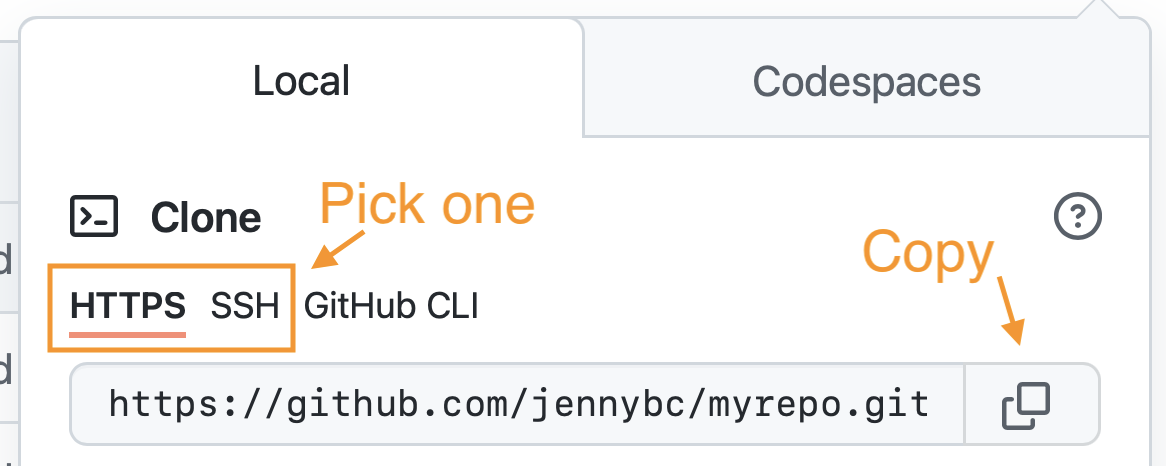
\includegraphics[width=0.6\linewidth]{img/github-https-or-ssh-url-annotated} \end{center}

\section{Clone the repo to your local computer}\label{git-clone-command-line}

We have a few ways to do this.
Here we use command line Git.
In section \ref{new-github-first}, we show other methods that you might prefer in daily life:
using usethis or the RStudio IDE.

Go to the shell (Appendix \ref{shell}).

Take charge of -- or at least notice! -- what directory you're in.
\texttt{pwd} displays the working directory.
\texttt{cd} is the command to change directory.
Personally, I would do this sort of thing in \texttt{\textasciitilde{}/tmp}.

Clone \texttt{myrepo} from GitHub to your computer.
Use the URL we just copied from GitHub.
This URL should have \textbf{your GitHub username} and the name of \textbf{your practice repo}.
If your shell (Appendix \ref{shell}) cooperates, you should be able to paste the whole \texttt{https://....} bit that we copied above.
But some shells are not (immediately) clipboard aware.
In that sad case, you must type it. \textbf{Accurately.}

\begin{Shaded}
\begin{Highlighting}[]
\NormalTok{git clone https://github.com/YOUR{-}USERNAME/YOUR{-}REPOSITORY.git}
\end{Highlighting}
\end{Shaded}

This should look something like this:

\begin{Shaded}
\begin{Highlighting}[]
\NormalTok{\textasciitilde{}/tmp \% git clone https://github.com/jennybc/myrepo.git}
\NormalTok{Cloning into \textquotesingle{}myrepo\textquotesingle{}...}
\NormalTok{remote: Enumerating objects: 3, done.}
\NormalTok{remote: Counting objects: 100\% (3/3), done.}
\NormalTok{remote: Total 3 (delta 0), reused 0 (delta 0), pack{-}reused 0}
\NormalTok{Receiving objects: 100\% (3/3), done.}
\end{Highlighting}
\end{Shaded}

Make this new repo your working directory, list its files, display the README, and get some information on its connection to GitHub:

\begin{Shaded}
\begin{Highlighting}[]
\NormalTok{cd myrepo}
\NormalTok{ls}
\NormalTok{head README.md}
\NormalTok{git remote show origin}
\end{Highlighting}
\end{Shaded}

This should look something like this:

\begin{Shaded}
\begin{Highlighting}[]
\ExtensionTok{\textasciitilde{}/tmp}\NormalTok{ \% cd myrepo}

\ExtensionTok{\textasciitilde{}/tmp/myrepo}\NormalTok{ \% ls}
\ExtensionTok{README.md}

\ExtensionTok{\textasciitilde{}/tmp/myrepo}\NormalTok{ \% head README.md }
\CommentTok{\# myrepo}
\ExtensionTok{checking}\NormalTok{ stuff for Happy Git}

\ExtensionTok{\textasciitilde{}/tmp/myrepo}\NormalTok{ \% git remote show origin}
\ExtensionTok{*}\NormalTok{ remote origin}
  \ExtensionTok{Fetch}\NormalTok{ URL: https://github.com/jennybc/myrepo.git}
  \ExtensionTok{Push}\NormalTok{  URL: https://github.com/jennybc/myrepo.git}
  \ExtensionTok{HEAD}\NormalTok{ branch: main}
  \ExtensionTok{Remote}\NormalTok{ branch:}
    \ExtensionTok{main}\NormalTok{ tracked}
  \ExtensionTok{Local}\NormalTok{ branch configured for }\StringTok{\textquotesingle{}git pull\textquotesingle{}}\NormalTok{:}
    \ExtensionTok{main}\NormalTok{ merges with remote main}
  \ExtensionTok{Local}\NormalTok{ ref configured for }\StringTok{\textquotesingle{}git push\textquotesingle{}}\NormalTok{:}
    \ExtensionTok{main}\NormalTok{ pushes to main }\ErrorTok{(}\ExtensionTok{up}\NormalTok{ to date}\KeywordTok{)}
\end{Highlighting}
\end{Shaded}

\section{Make a local change, commit, and push}\label{make-a-local-change-commit-and-push}

Add a line to README and verify that Git notices the change:

\begin{Shaded}
\begin{Highlighting}[]
\NormalTok{echo "A line I wrote on my local computer  " \textgreater{}\textgreater{} README.md}
\NormalTok{git status}
\end{Highlighting}
\end{Shaded}

This should look something like this:

\begin{Shaded}
\begin{Highlighting}[]
\NormalTok{\textasciitilde{}/tmp/myrepo \% echo "A line I wrote on my local computer" \textgreater{}\textgreater{} README.md}

\NormalTok{\textasciitilde{}/tmp/myrepo \% git status}
\NormalTok{On branch main}
\NormalTok{Your branch is up to date with \textquotesingle{}origin/main\textquotesingle{}.}

\NormalTok{Changes not staged for commit:}
\NormalTok{  (use "git add \textless{}file\textgreater{}..." to update what will be committed)}
\NormalTok{  (use "git restore \textless{}file\textgreater{}..." to discard changes in working directory)}
\NormalTok{        modified:   README.md}

\NormalTok{no changes added to commit (use "git add" and/or "git commit {-}a")}
\end{Highlighting}
\end{Shaded}

Stage (``add'') and commit this change and push to your remote repo on GitHub.

If you're a new GitHub user and using HTTPS, you might be challenged for your username and password.
Even though GitHub no longer allows username/password authentication, many general Git tools still frame the authentication task with this vocabulary.
By all means, provide your GitHub username when prompted.
However, the most critical piece is to \textbf{provide your PAT as the password}.
Do not enter your web password.
Enter your PAT.
If you already stored your PAT with \texttt{gitcreds::gitcreds\_set()}, it should be discovered automatically and you will not see a credential challenge.

\begin{Shaded}
\begin{Highlighting}[]
\NormalTok{git add README.md}
\NormalTok{git commit {-}m "A commit from my local computer"}
\NormalTok{git push}
\end{Highlighting}
\end{Shaded}

This should look something like this:

\begin{Shaded}
\begin{Highlighting}[]
\NormalTok{\textasciitilde{}/tmp/myrepo \% git add README.md}

\NormalTok{\textasciitilde{}/tmp/myrepo \% git commit {-}m "A commit from my local computer"}
\NormalTok{[main e92528c] A commit from my local computer}
\NormalTok{ 1 file changed, 1 insertion(+)}
 
\NormalTok{\textasciitilde{}/tmp/myrepo \% git push}
\NormalTok{Enumerating objects: 5, done.}
\NormalTok{Counting objects: 100\% (5/5), done.}
\NormalTok{Delta compression using up to 12 threads}
\NormalTok{Compressing objects: 100\% (2/2), done.}
\NormalTok{Writing objects: 100\% (3/3), 327 bytes | 327.00 KiB/s, done.}
\NormalTok{Total 3 (delta 0), reused 0 (delta 0), pack{-}reused 0}
\NormalTok{To https://github.com/jennybc/myrepo.git}
\NormalTok{   31dcaef..e92528c  main {-}\textgreater{} main}
\end{Highlighting}
\end{Shaded}

Do you see an error like this?

\begin{Shaded}
\begin{Highlighting}[]
\NormalTok{\textasciitilde{}/tmp/myrepo \% git push                                                     }
\NormalTok{remote: Support for password authentication was removed on August 13, 2021. Please use a personal access token instead.}
\NormalTok{remote: Please see https://github.blog/2020{-}12{-}15{-}token{-}authentication{-}requirements{-}for{-}git{-}operations/ for more information.}
\NormalTok{fatal: Authentication failed for \textquotesingle{}https://github.com/jennybc/myrepo.git/\textquotesingle{}}
\end{Highlighting}
\end{Shaded}

This means you have provided your GitHub \emph{web password}, instead of your \emph{personal access token} (PAT).
Go back to chapter \ref{https-pat} to get a PAT.
Try \texttt{git\ push} again and hopefully you'll get another prompt, allowing you to correct things and provide your PAT.

If you ever feel you need to overwrite a bad credential with a new one, the easiest way to do this is to call \texttt{gitcreds::gitcreds\_set()} from R.

\subsection{Windows and line endings}\label{windows-and-line-endings}

On Windows, you might see a message about \texttt{LF\ will\ be\ replaced\ by\ CRLF}. This is normal and does not require any action on your part.
Windows handles line endings differently from other operating systems, but the default setup for Git for Windows is appropriate for most people and situations.

Here's a command to reveal the current line ending configuration and some typical output \textbf{on Windows}:

\begin{Shaded}
\begin{Highlighting}[]
\NormalTok{$ git config {-}{-}show{-}origin {-}{-}get core.autocrlf}
\NormalTok{file:"C:\textbackslash{}\textbackslash{}ProgramData/Git/config"      true}
\end{Highlighting}
\end{Shaded}

If your value shows as \texttt{false}, you can set it to \texttt{true} with this command:

\begin{Shaded}
\begin{Highlighting}[]
\NormalTok{$ git config {-}{-}global core.autocrlf true}
\end{Highlighting}
\end{Shaded}

\texttt{true} is the current default setting for \texttt{core.autocrlf} for \hyperref[install-git-windows]{Git for Windows}, our recommended method for installing Git on Windows.
The need to set this explicitly in your global user config suggests you should consider reinstalling or updating Git for Windows.

\section{Confirm the local change propagated to the GitHub remote}\label{confirm-the-local-change-propagated-to-the-github-remote}

Go back to the browser.
I assume we're still viewing your new GitHub repo.

Refresh.

You should see the new ``A line I wrote on my local computer'' in the README.

If you click on ``commits,'' you should see one with the message ``A commit from my local computer.''

If you have made it this far, you and your test repo are ready to graduate to using Git and GitHub with RStudio (chapter \ref{rstudio-git-github}).

\section{Clean up}\label{clean-up}

If you're ready to conclude this test of your Git installation and GitHub configuration, we can clean up the test repository now.

\textbf{Local} When you're ready to clean up, you can delete the local repo any way you like. It's just a regular directory on your computer.

Here's how to do that in the shell, if current working directory is \texttt{myrepo}:

\begin{Shaded}
\begin{Highlighting}[]
\NormalTok{cd ..}
\NormalTok{rm {-}rf myrepo/}
\end{Highlighting}
\end{Shaded}

\textbf{GitHub} In the browser, go to your repo's landing page on GitHub.
Click on ``Settings''.

Scroll down, click on ``delete repository,'' and do as it asks.

\chapter{Connect RStudio to Git and GitHub}\label{rstudio-git-github}

Here we verify that RStudio can issue Git commands on your behalf.
Assuming that you've gotten local Git to talk to GitHub, this means you'll also be able to pull from and push to GitHub from RStudio.

In later chapters and in live workshops, we revisit these operations with much more explanation.

If you succeed here, your set up is DONE.

\section{Prerequisites}\label{prerequisites}

We assume the following:

\begin{itemize}
\tightlist
\item
  You've registered a free GitHub account (chapter \ref{github-acct}).
\item
  You've installed/updated R and RStudio (chapter \ref{install-r-rstudio}).
\item
  You've installed Git (chapter \ref{install-git}).
\item
  You've introduced yourself to Git (chapter \ref{hello-git}).
\item
  You've confirmed that you can push to / pull from GitHub from the command line (chapter \ref{push-pull-github}).
\end{itemize}

You will also need a test repository on GitHub.
If you don't have a suitable test repository on GitHub, follow the instructions in the next section.

If you just completed the previous chapter, \hyperref[push-pull-github]{Connect to GitHub}, that repo will be perfect!
However, I encourage you to delete the \emph{local} repository, so you can experience how we use RStudio to clone it and get a local copy.
This is a actually a workflow we refer to elsewhere (see \ref{burn} as ``burn it all down''.
It's a deeply pragmatic coping strategy if your local Git repo is goofed up, but the version on GitHub is pretty current.

Delete the folder corresponding to the \textbf{local repo} any way you like.
It's just a regular directory on your computer.
Here's how to do that in the shell, if current working directory is \texttt{myrepo}:

\begin{Shaded}
\begin{Highlighting}[]
\NormalTok{cd ..}
\NormalTok{rm {-}rf myrepo/}
\end{Highlighting}
\end{Shaded}

\section{Make a repo on GitHub}\label{make-a-repo-on-github-1}

Go to \url{https://github.com} and make sure you are logged in.

Near ``Repositories'', click the big green ``New'' button.
Or, if you are on your own profile page, click on ``Repositories'', then click the big green ``New'' button.

How to fill this in:

\begin{itemize}
\tightlist
\item
  Repository template: No template.
\item
  Repository name: \texttt{myrepo} or whatever you wish (we'll delete this soon).
\item
  Description: ``Repository for testing my Git/GitHub setup'' or similar. It's nice to have something here, so you'll see it appear in the README.
\item
  Public.
\item
  Initialize this repository with: Add a README file.
\end{itemize}

Click the big green button that says ``Create repository''.

Now click the big green button that says ``\textless\textgreater{} Code''.

Copy a clone URL to your clipboard.
If you're taking our default advice, copy the HTTPS URL.
But if you're opting for SSH, then make sure to copy the SSH URL.

\begin{center}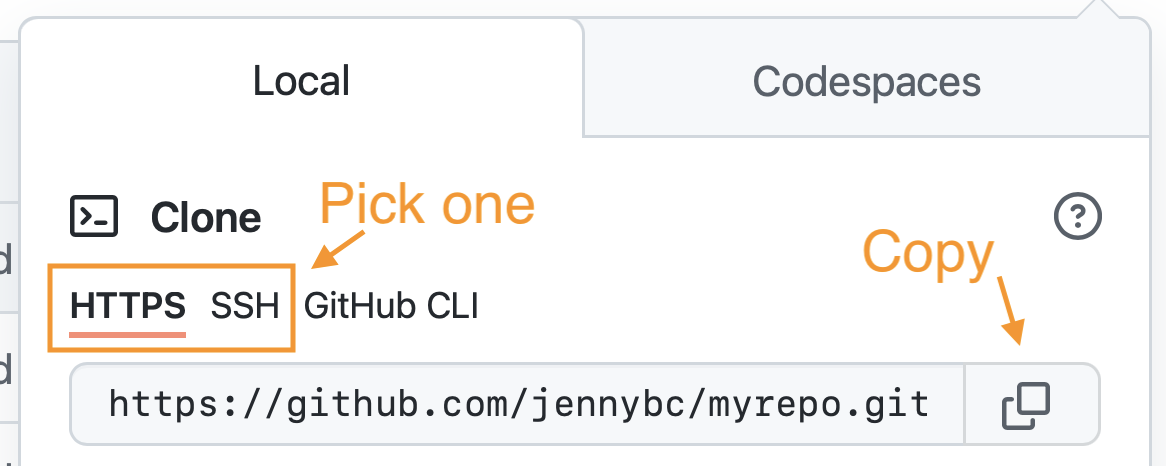
\includegraphics[width=0.6\linewidth]{img/github-https-or-ssh-url-annotated} \end{center}

\section{Clone the test GitHub repository to your computer via RStudio}\label{clone-the-test-github-repository-to-your-computer-via-rstudio}

In RStudio, start a new Project:

\begin{itemize}
\tightlist
\item
  \emph{File \textgreater{} New Project \textgreater{} Version Control \textgreater{} Git}. In ``Repository URL'', paste the URL of your new GitHub repository. It will be something like this \texttt{https://github.com/jennybc/myrepo.git}.

  \begin{itemize}
  \tightlist
  \item
    Do you NOT see an option to get the Project from Version Control? Restart RStudio and try again. Still no luck? Go to chapter \ref{rstudio-see-git} for tips on how to help RStudio find Git.
  \end{itemize}
\item
  Accept the default project directory name, e.g.~\texttt{myrepo}, which coincides with the GitHub repo name.
\item
  Take charge of -- or at least notice! -- where the Project will be saved locally. A common rookie mistake is to have no idea where you are saving files or what your working directory is. Pay attention. Be intentional. Personally, I would do this in \texttt{\textasciitilde{}/tmp}.
\item
  I suggest you check ``Open in new session'', as that's what you'll usually do in real life.
\item
  Click ``Create Project''.
\end{itemize}

You should find yourself in a new local RStudio Project that represents your test repo on GitHub.
This should download the \texttt{README.md} file from GitHub.
Look in RStudio's file browser pane for the \texttt{README.md} file.

\section{Make local changes, save, commit}\label{make-local-changes-save-commit}

From RStudio, modify the \texttt{README.md} file, e.g., by adding the line ``This is a line from RStudio''. Save your changes.

Commit these changes to your local repo. How?

From RStudio:

\begin{itemize}
\tightlist
\item
  Click the ``Git'' tab in upper right pane.
\item
  Check ``Staged'' box for \texttt{README.md}.
\item
  If you're not already in the Git pop-up, click ``Commit''.
\item
  Type a message in ``Commit message'', such as ``Commit from RStudio''.
\item
  Click ``Commit''.
\end{itemize}

\section{Push your local changes online to GitHub}\label{push-your-local-changes-online-to-github}

Click the green ``Push'' button to send your local changes to GitHub.

You should not experience a credential challenge, since one of the pre-requisites was successfully pushing to GitHub from the command line (chapter \ref{push-pull-github}).
RStudio's Git pane just exposes a specific subset of command line Git and therefore once your credentials work in the shell, they should work in RStudio.
If you do experience a credential challenge, that suggests you should have a look at the troubleshooting suggestions for your chosen protocol, either \hyperref[pat-troubleshooting]{HTTPS} or \hyperref[ssh-troubleshooting]{SSH}.

\section{Confirm the local change propagated to the GitHub remote}\label{confirm-the-local-change-propagated-to-the-github-remote-1}

Go back to the browser.
I assume we're still viewing your new GitHub repo.

Refresh.

You should see the new ``This is a line from RStudio'' in the README.

If you click on ``commits'', you should see one with the message ``Commit from RStudio''.

If you have made it this far, you are DONE with set up.
Congratulations!

\section{Clean up}\label{clean-up-1}

Quit the RStudio instance that's open to your test Project / Git repo.

Delete the local repo any way you like.
It's just a regular directory on your computer.

Here's how to do that in the shell, if current working directory is \texttt{myrepo}:

\begin{Shaded}
\begin{Highlighting}[]
\NormalTok{cd ..}
\NormalTok{rm {-}rf myrepo/}
\end{Highlighting}
\end{Shaded}

In the browser, go to your repo's landing page on GitHub.
Click on ``Settings''.

Scroll down, click on ``delete repository,'' and do as it asks.

\chapter{Detect Git from RStudio}\label{rstudio-see-git}

If you want RStudio to help with your Git and GitHub work, it must be able to find the Git executable.

This usually ``just works'', so this page is aimed at people who have reason to suspect they have a problem.

This is something you set up once-per-computer.

\section{Do you have a problem?}\label{do-you-have-a-problem}

Let's check if RStudio can find the Git executable.

\begin{itemize}
\tightlist
\item
  \emph{File \textgreater{} New Project\ldots{}} Do you see an option to create from Version Control? If yes, good.
\item
  Select \emph{New Directory} \textgreater{} \emph{Empty Project}. Do you see a checkbox ``Create a git repository''? If yes, good, CHECK IT.
\end{itemize}

Keep reading if things don't go so well or you want to know more.

\section{Find Git yourself}\label{find-git-yourself}

RStudio can only act as a GUI front-end for Git if Git has been successfully installed (chapter \ref{install-git}) \textbf{AND RStudio can find it}.

A basic test for successful installation of Git is to simply enter \texttt{git} in the shell (Appendix \ref{shell}).
If you get a complaint about Git not being found, it means installation was unsuccessful or that it is not being found, i.e.~it is not on your \texttt{PATH}.

If you are not sure where the Git executable lives, try this in a shell:

\begin{itemize}
\item
  \texttt{which\ git} (Mac, Linux, Git Bash shell on Windows)
\item
  \texttt{where\ git} (Windows command prompt, i.e.~\texttt{cmd.exe})
\end{itemize}

\section{Tell RStudio where to find Git}\label{tell-rstudio-where-to-find-git}

If Git appears to be installed and findable, launch RStudio.
Quit and re-launch RStudio if there's \textbf{any doubt in your mind} about whether you opened RStudio before or after installing Git.
Don't make me stop this car and restart RStudio for you in office hours.
DO IT.

From RStudio, go to \emph{Tools \textgreater{} Global Options \textgreater{} Git/SVN} and make sure that the box \emph{Git executable} points to your Git executable.

On macOS and Linux, the path usually looks something like this:

\begin{Shaded}
\begin{Highlighting}[]
\NormalTok{/usr/bin/git}
\end{Highlighting}
\end{Shaded}

If you need to set this on macOS, it can sometimes be hard to navigate to the necessary directory, once you've clicked ``Browse'' and are working with a Finder-type window.
The keyboard shortcut ``command + shift + g'' will summon ``Go To Folder'', where you will be able to type or paste any path you want.

On Windows, this path should look something like this:

\begin{Shaded}
\begin{Highlighting}[]
\ExtensionTok{C:/Program}\NormalTok{ Files/Git/bin/git.exe}
\end{Highlighting}
\end{Shaded}

and here is a screenshot on Windows:

\begin{center}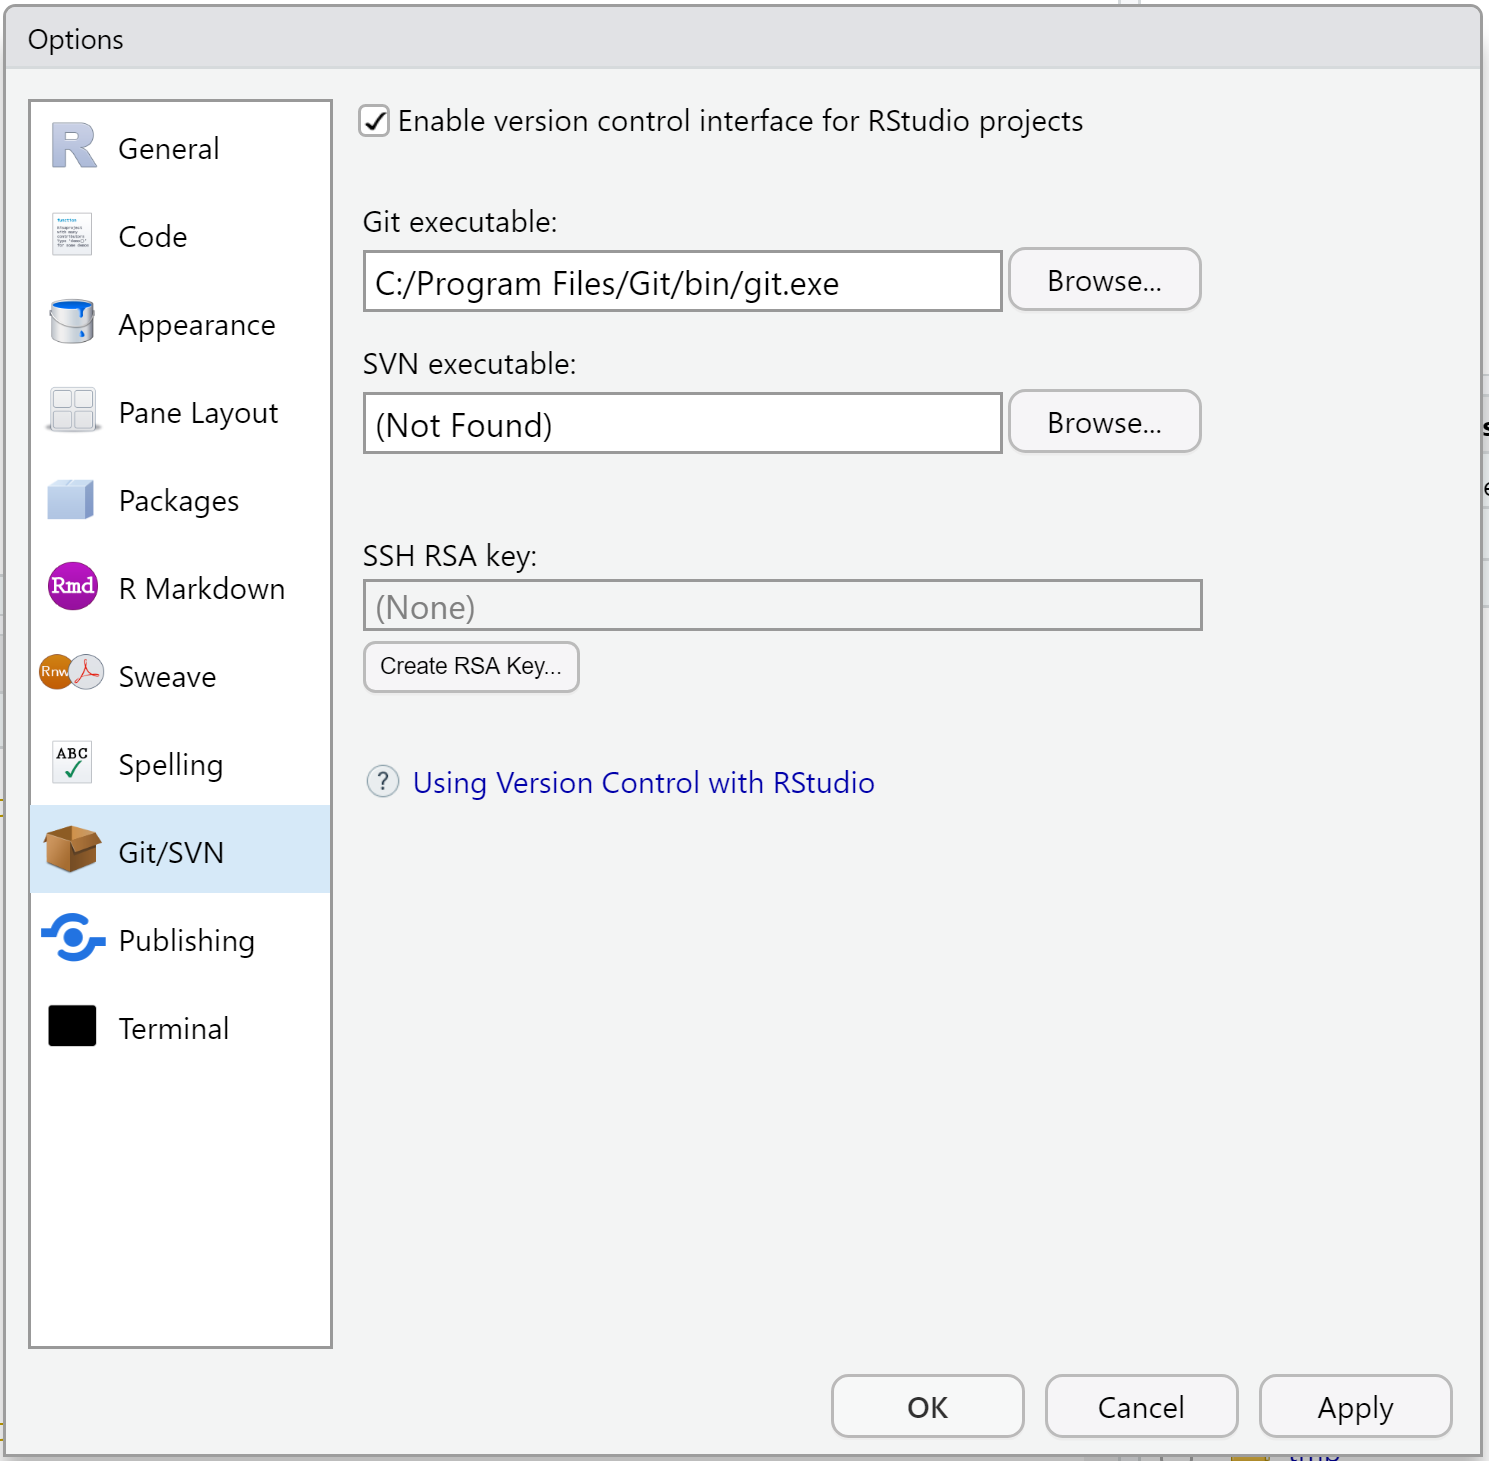
\includegraphics[width=1\linewidth]{img/windows-rstudio-git-executable-screenshot} \end{center}

\textbf{WARNING}: On Windows, do \textbf{NOT} use \texttt{C:/Program\ Files/Git/cmd/git.exe}. \texttt{bin} in the path is GOOD YES!
\texttt{cmd} in the path is BAD NO!

\textbf{WARNING}: On Windows, do \textbf{NOT} set this to \texttt{git-bash.exe}.
Something that ends in \texttt{git.exe} is GOOD YES! \texttt{git-bash.exe} is BAD NO!

\textbf{Restart RStudio if you make any changes here.}
Don't make me stop this car again and restart RStudio for you in office hours.
DO IT.

Re-do the steps at the top of the page to see if RStudio and Git are communicating now.

No joy?

\begin{itemize}
\item
  I've seen this help: With your Project open, go to \texttt{Tools\ \textgreater{}\ Project\ Options...}. If available, click on ``Git/SVN'' and select ``Git'' in the Version control system dropdown menu. Answer ``yes'' to the ``Confirm New Git Repository'' pop up. Answer ``yes'' to the ``Confirm Restart RStudio'' pop up.
\item
  If you installed Git via GitHub for Windows, it is possible the Git executable is really well hidden. Get help or use one of \hyperref[install-git]{our recommended methods of installing Git}.
\item
  Your \texttt{PATH} is probably not set up correctly and/or you should re-install Git and control/notice where it's going. Read more in \ref{troubleshooting}.
\item
  Get our help.
\end{itemize}

\chapter{RStudio, Git, GitHub Hell}\label{troubleshooting}

Problems we have seen and possible solutions.

If you experience some new problem and, especially, find the corresponding solution, \href{https://github.com/jennybc/happy-git-with-r/issues}{we'd love to hear from you!}

\section{I think I have installed Git but damn if I can find it}\label{i-think-i-have-installed-git-but-damn-if-i-can-find-it}

When you install Git, try to control or record where it is being installed!
Make a mental or physical note of these things.

You may be able to find Git after the fact with these commands in the shell (Appendix \ref{shell}):

\begin{itemize}
\item
  \texttt{which\ git} (Mac, Linux, or anything running a bash shell)
\item
  \texttt{where\ git} (Windows, when not in a bash shell)
\end{itemize}

It is not entirely crazy to just re-install Git, using a method that leaves it in a more conventional location, and to pay very close attention to where it's being installed.
Live and learn.

\section{RStudio Git pane disappears on Mac OS}\label{rstudio-git-pane-disappears-on-mac-os}

Sometimes the RStudio Git pane disappears on a system where it was previously working.
This usually happens to people who installed Git by installing the Xcode command line tools.
It is usually a sign that you need to re-agree to the Xcode license agreement. This is necessary after a Mac OS upgrade, re-installing Xcode, or even quiet Xcode upgrades that sometimes seem to happen without the user's knowledge.

In the shell, you could execute \texttt{git\ status} and you might see a message along these lines:

\begin{Shaded}
\begin{Highlighting}[]
\NormalTok{Agreeing to the Xcode/iOS license requires admin privileges, please run “sudo xcodebuild {-}license” and then retry this command.}
\end{Highlighting}
\end{Shaded}

If you get such clear instructions, by all means do what it says, i.e.~run \texttt{sudo\ xcodebuild\ -license}, to re-agree to the license.

In any case, you need to tickle the Xcode command line tools to prompt you for whatever it needs. Here are other commands that, depending on the situation, might trigger the necessary prompts:

\begin{Shaded}
\begin{Highlighting}[]
\NormalTok{xcode{-}select {-}{-}install}
\end{Highlighting}
\end{Shaded}

or

\begin{Shaded}
\begin{Highlighting}[]
\NormalTok{git config {-}{-}global {-}{-}list}
\end{Highlighting}
\end{Shaded}

Then \textbf{restart RStudio}.

\section{Dysfunctional PATH}\label{dysfunctional-path}

Some cases of RStudio \emph{not} automatically detecting the Git executable stem from problems with \texttt{PATH}.
This is the set of directories where your computer will look for executables, such as Git (today) or \texttt{make}.
Certain methods of Git installation, especially on Windows and/or older OSes, have a higher tendency to put Git in an unconventional location or to fail to add the relevant directory to \texttt{PATH}.

How to see your \texttt{PATH}?

In the shell:

\begin{Shaded}
\begin{Highlighting}[]
\NormalTok{echo $PATH}
\end{Highlighting}
\end{Shaded}

Take a good hard look at this.
See the point above about finding your Git executable or re-installing it while you are \textbf{wide awake}.
Is the Git executable's parent directory in your \texttt{PATH}?
No?
\textbf{Fix that.}

At this point I recommend that you do a Google search to find instructions on how to modify \texttt{PATH} on your specific operating system.

\section{Push/Pull buttons greyed out in RStudio}\label{pushpull-buttons-greyed-out-in-rstudio}

Are you sure your local repository is associated with a remote repository, e.g.~a GitHub repo?
In a shell with working directory set to the local Git repo, enter this command:

\begin{Shaded}
\begin{Highlighting}[]
\NormalTok{\textasciitilde{}/tmp/myrepo \% git remote {-}v                                           }
\NormalTok{origin  git@github.com:jennybc/myrepo.git (fetch)}
\NormalTok{origin  git@github.com:jennybc/myrepo.git (push)}
\end{Highlighting}
\end{Shaded}

We want to see that fetch and push are set to remote URLs that point to the remote repo.

If you discover you still need to set a remote, get the HTTPS or SSH URL, as appropriate, for your GitHub repo.
This is easy to get onto your clipboard from the repo's GitHub page.
Do this in the shell:

\begin{Shaded}
\begin{Highlighting}[]
\NormalTok{git remote add origin https://github.com/jennybc/myrepo.git}
\end{Highlighting}
\end{Shaded}

Download all the files from the online GitHub repository and deal with any
conflicts (substituting \texttt{master} for \texttt{main}, if relevant).

\begin{Shaded}
\begin{Highlighting}[]
\NormalTok{git pull origin main}
\end{Highlighting}
\end{Shaded}

Call \texttt{git\ remote\ -v} again.
Once you are satisfied that your GitHub remote is set properly, you can move on to the next step.

Are you sure the current branch is \emph{tracking} a branch on the remote?
In that same shell, in your repo, do this:

\begin{Shaded}
\begin{Highlighting}[]
\NormalTok{\textasciitilde{}/tmp/myrepo \% git branch {-}vv}
\NormalTok{* main 2899c91 [origin/main] A commit from my local computer}
\end{Highlighting}
\end{Shaded}

The above shows successful confirmation that the local \texttt{main} branch is tracking \texttt{origin/main}, i.e.~the \texttt{main} branch on GitHub.
If you don't see the \texttt{{[}origin/main{]}} bit, that is a problem.
By the way, \texttt{git\ branch\ -r} and \texttt{git\ remote\ show\ origin} are two more commands that are helpful for examining your remote setup.

When connecting a local repo to a new GitHub repo, a lot of people remember to add the GitHub remote, but forget to also cement this tracking relationship for any relevant branches.

If you discover your local \texttt{main} branch is not yet tracking \texttt{main} on GitHub, fix that like so:

\begin{Shaded}
\begin{Highlighting}[]
\NormalTok{git push {-}{-}set{-}upstream origin main}
\end{Highlighting}
\end{Shaded}

This is equivalent to \texttt{git\ push\ -u\ origin\ main} but conveys more about what you are doing.

Call \texttt{git\ branch\ -vv} or \texttt{git\ branch\ -r} or \texttt{git\ remote\ show\ origin} again to confirm that the \texttt{main} branch on GitHub is the tracking branch for the local \texttt{main} branch.

\section{I have no idea if my local repo and my remote repo are connected.}\label{i-have-no-idea-if-my-local-repo-and-my-remote-repo-are-connected.}

See the above section on ``Push/Pull buttons greyed out in RStudio.''

\section{Push rejected, i.e.~fail at the Git/GitHub level}\label{push-rejected-i.e.-fail-at-the-gitgithub-level}

You might have changes on the remote AND on your local repo.
Just because you don't remember making any edits in the browser doesn't mean you didn't.
Humor me.

Pull first.
Resolve any conflicts.
Then try your push again.

\section{RStudio is not making certain files available for staging/committing}\label{rstudio-is-not-making-certain-files-available-for-stagingcommitting}

Do you have a space in your directory or file names? \href{https://twitter.com/aaronquinlan/status/711593127551733761}{A space in a file name is a space in your soul.}
Get rid of it.

Is your Git repo / RStudio Project inside a folder that \ldots{} eventually rolls up to Google Drive, DropBox, Microsoft OneDrive, or a network drive?
If yes, I recommend you move the repo / Project into a plain old directory that lives directly on your computer and that is not managed by, e.g., Google Drive.

If you cannot deal with the two root causes identified above, then it is possible that a more powerful Git client (chapter \ref{git-client}) will be able to cope with these situations.
But I make no promises.
You should also try Git operations from the command line.

\section{I hear you have some Git repo inside your Git repo}\label{i-hear-you-have-some-git-repo-inside-your-git-repo}

Do not create a Git repository inside another Git repository. Just don't.

If you have a genuine need for this, which is really rare, the proper way to do it is via \href{http://git-scm.com/book/en/v2/Git-Tools-Submodules}{submodules}.

In STAT 545, we certainly do not need to do this and when we've seen it, it's been a mistake.
This has resulted in the unexpected and complete loss of the inner Git repository.
To be sure, there was more going on here (cough, GitHub Desktop client), but non-standard usage of Git repos makes it much easier to make costly mistakes.

\part{Early GitHub Wins}\label{part-early-github-wins}

\chapter*{Get started with GitHub}\label{usage-intro}
\addcontentsline{toc}{chapter}{Get started with GitHub}

Now that we've verified your Git/GitHub/RStudio setup, we can demo the workflows you'll use to get your work onto GitHub:

\begin{itemize}
\tightlist
\item
  \hyperref[new-github-first]{New project, GitHub first} is the easiest way to get a working project.
\item
  \hyperref[existing-github-first]{Existing project, GitHub first} is a deeply pragmatic way to get pre-existing work onto GitHub.
\item
  \hyperref[existing-github-last]{Existing project, GitHub last} is the more proper way to connect existing local work to a remote on GitHub, especially if there's already a Git history.
\end{itemize}

This part concludes with two R-specific workflows that show off how well \href{https://rmarkdown.rstudio.com}{R Markdown (the format)} and \href{https://cran.r-project.org/package=rmarkdown}{rmarkdown (the package)} work with GitHub:

\begin{itemize}
\tightlist
\item
  \hyperref[rmd-test-drive]{Test drive R Markdown}
\item
  \hyperref[r-test-drive]{Render an R script}
\end{itemize}

\chapter{New project, GitHub first}\label{new-github-first}

We create a new Project, with the preferred ``GitHub first, then RStudio'' sequence.
Why do we prefer this?
Because this method of copying the Project from GitHub to your computer also sets up the local Git repository for immediate pulling and pushing.
Under the hood, we are doing \texttt{git\ clone}.

You've actually done this before during set up (chapter \ref{rstudio-git-github}).
We're doing it again, \emph{with feeling}.

The workflow is pretty similar for other repository managers like GitLab or Bitbucket.
We will specify below when you may need to do something differently.

\section{Make a repo on GitHub}\label{make-a-repo-on-github-2}

Go to \url{https://github.com} and make sure you are logged in.

Near ``Repositories'', click the big green ``New'' button.
Or, if you are on your own profile page, click on ``Repositories'', then click the big green ``New'' button.

How to fill this in:

\begin{itemize}
\tightlist
\item
  Repository template: No template.
\item
  Repository name: \texttt{myrepo} or whatever you wish to name your new project. Approach this similar to a variable name, in code: descriptive but brief, no whitespace. Letters, digits, \texttt{-}, \texttt{.}, or \texttt{\_} are allowed.
\item
  Description: ``Analysis of the stuff'' or any short description of the project. Write this for humans.
\item
  Public.
\item
  Initialize this repository with: Add a README file.
\end{itemize}

Click the big green button that says ``Create repository''.

Now click the big green button that says ``\textless\textgreater{} Code''.

Copy a clone URL to your clipboard.
If you're taking our default advice, copy the HTTPS URL.
But if you're opting for SSH, then make sure to copy the SSH URL.

\begin{center}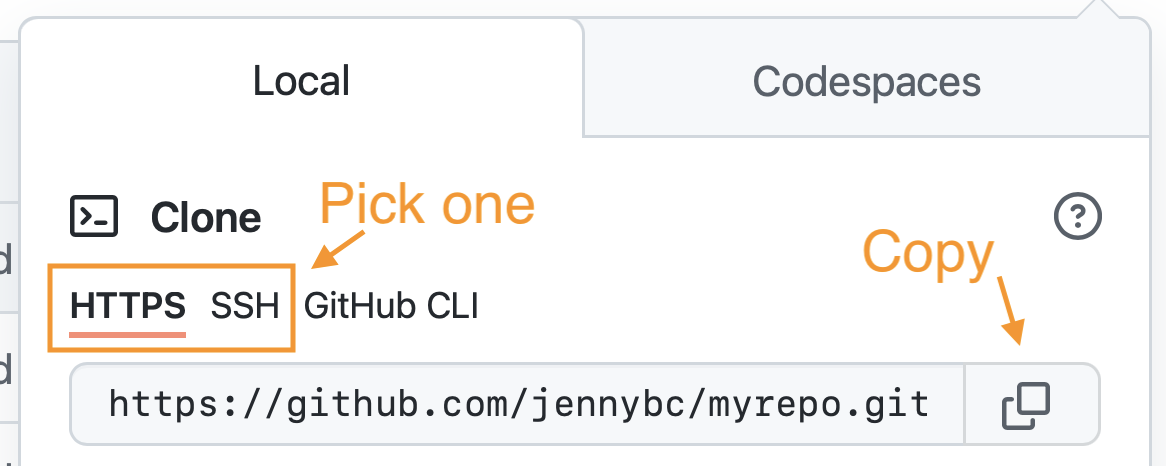
\includegraphics[width=0.6\linewidth]{img/github-https-or-ssh-url-annotated} \end{center}

\subsection{GitLab}\label{gitlab}

Log in at \url{https://gitlab.com}.
Click on the ``+'' button in the top-right corner, and then on ``New project''.

\begin{itemize}
\tightlist
\item
  Project name: \texttt{myrepo} (or whatever you wish)\\
\item
  Public
\item
  YES Initialize repository with a README
\end{itemize}

Click the big green button ``Create project.''

Copy the HTTPS or SSH clone URL to your clipboard via the blue ``Clone'' button.

\subsection{Bitbucket}\label{bitbucket}

Log in at \url{https://bitbucket.org}.
On the left-side pane, click on the ``+'' button, and then on ``Repository'' under ``Create''.

\begin{itemize}
\tightlist
\item
  Repository name: \texttt{myrepo} (or whatever you wish)
\item
  Access level: Uncheck to make the repository public.
\item
  Include a README?: Select either ``Yes, with a tutorial (for beginners)'' or ``Yes, with a template''
\item
  Version control system: Git
\end{itemize}

Click the big blue button ``Create repository.''

Copy the HTTPS or SSH clone URL that appears when you click on the blue ``Clone'' button.
Make sure you remove the \texttt{git\ clone\ ...} that shows up at the beginning.

\section{New RStudio Project via git clone}\label{new-rstudio-project-via-git}

\begin{center}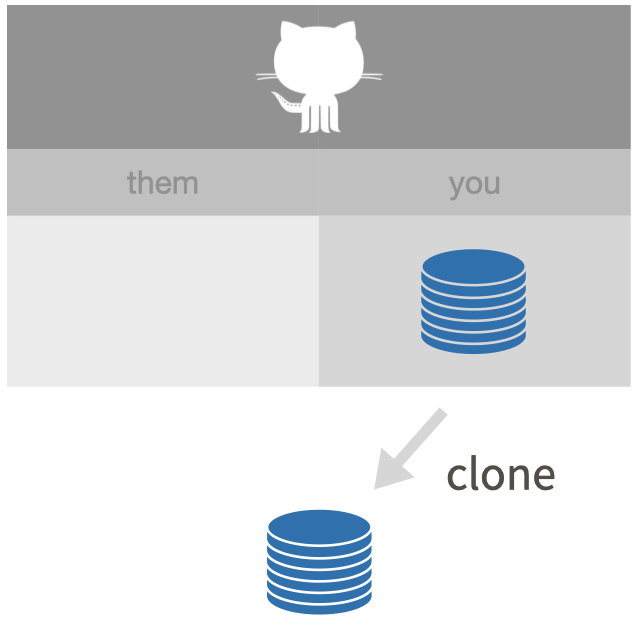
\includegraphics[width=0.6\linewidth]{img/new-project-github-first} \end{center}

I present two ways to do this:

\begin{itemize}
\tightlist
\item
  \texttt{usethis::create\_from\_github()}
\item
  Via the RStudio IDE
\end{itemize}

\emph{(Recall that we showed how to do this with command line Git in chapter \ref{push-pull-github}.)}

When you are cloning your own GitHub repository, the two methods are equivalent.
In other scenarios, especially fork-and-clone (chapter \ref{fork-and-clone}), I think \texttt{usethis::create\_from\_github()} is superior, because it does additional, recommended setup.

Pick \textbf{one} of these methods below.

\subsection{\texorpdfstring{\texttt{usethis::create\_from\_github()}}{usethis::create\_from\_github()}}\label{usethiscreate_from_github}

You can execute this command in any R session.
If you use RStudio, then do this in the R console of any RStudio instance.

\begin{Shaded}
\begin{Highlighting}[]
\NormalTok{usethis}\SpecialCharTok{::}\FunctionTok{create\_from\_github}\NormalTok{(}
  \StringTok{"https://github.com/YOU/YOUR\_REPO.git"}\NormalTok{,}
  \AttributeTok{destdir =} \StringTok{"\textasciitilde{}/path/to/where/you/want/the/local/repo/"}
\NormalTok{)}
\end{Highlighting}
\end{Shaded}

The first argument is \texttt{repo\_spec} and it accepts the GitHub repo specification in various forms.
In particular, you can use the URL we just copied from GitHub.

The \texttt{destdir} argument specifies the parent directory where you want the new folder (and local Git repo) to live.
If you don't specify \texttt{destdir}, usethis defaults to some very conspicuous place, like your desktop.
If you like to keep Git repos in a certain folder on your computer, you can personalize this default by setting the \texttt{usethis.destdir} option in your \texttt{.Rprofile}.

We're accepting the default behaviour of two other arguments, \texttt{rstudio} and \texttt{open}, because that's what most people will want.
For example, for an RStudio user, \texttt{create\_from\_github()} does this:

\begin{itemize}
\tightlist
\item
  Creates a new local directory in \texttt{destdir}, which is all of these things:

  \begin{itemize}
  \tightlist
  \item
    a directory or folder on your computer
  \item
    a Git repository, linked to a remote GitHub repository
  \item
    an RStudio Project
  \end{itemize}
\item
  Opens a new RStudio instance in the new Project
\item
  \textbf{In the absence of other constraints, I suggest that all of your R projects have exactly this set-up.}
\end{itemize}

\subsection{RStudio IDE}\label{rstudio-ide}

In RStudio, start a new Project:

\begin{itemize}
\tightlist
\item
  \emph{File \textgreater{} New Project \textgreater{} Version Control \textgreater{} Git}. In the ``repository URL'' paste
  the URL of your new GitHub repository. It will be something like this
  \texttt{https://github.com/jennybc/myrepo.git}.
\item
  Be intentional about where you create this Project.
\item
  I suggest you ``Open in new session''.
\item
  Click ``Create Project'' to create a new directory, which will be all of these things:

  \begin{itemize}
  \tightlist
  \item
    a directory or ``folder'' on your computer
  \item
    a Git repository, linked to a remote GitHub repository
  \item
    an RStudio Project
  \end{itemize}
\item
  \textbf{In the absence of other constraints, I suggest that all of your R projects have exactly this set-up.}
\end{itemize}

This should download the \texttt{README.md} file that we created on GitHub in the previous step.
Look in RStudio's file browser pane for the \texttt{README.md} file.

Behind the scenes, RStudio has done this for you:

\begin{Shaded}
\begin{Highlighting}[]
\NormalTok{git clone https://github.com/jennybc/myrepo.git}
\end{Highlighting}
\end{Shaded}

\subsection{Have a look around}\label{have-a-look-around}

Regardless of whether you used usethis or RStudio, you should now be working in the new Git repo.
The implicit \texttt{git\ clone} should download the \texttt{README.md} file that we created on GitHub in the previous step.
Look in RStudio's file browser pane for the \texttt{README.md} file.

There's a big advantage to the ``GitHub first, then RStudio'' workflow: the remote GitHub repo is configured as the \texttt{origin} remote for your local repo and your local \texttt{main} branch is now tracking the \texttt{main} on GitHub.
This is a technical but important point about Git.
The practical implication is that you are now set up to push and pull.
No need to fanny around setting up Git remotes and tracking branches on the command line.

We're about to confirm we are setup for pulling and pushing.

\begin{figure}
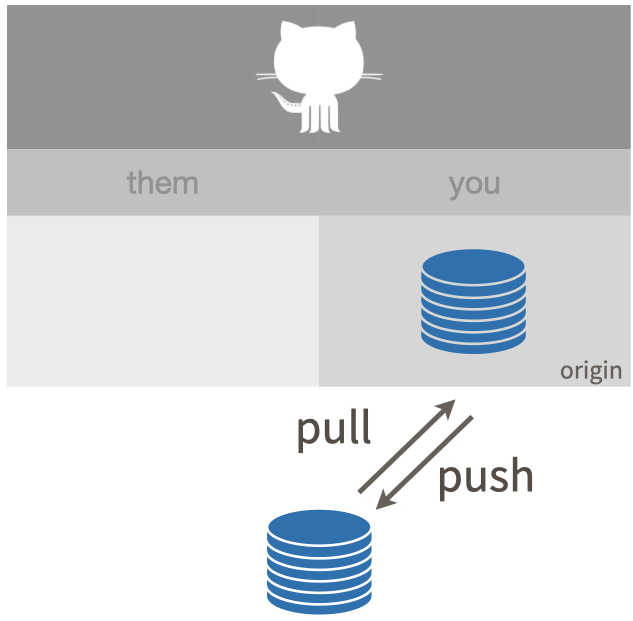
\includegraphics[width=0.6\linewidth]{img/github-pull-push} \caption{Pull and push.}\label{fig:github-pull-push}
\end{figure}

\subsection{Optional: peek under the hood}\label{optional-peek-under-the-hood}

Completely optional activity: use command line Git to see what we're talking about above, i.e.~the remote and tracking branch setup.

\texttt{git\ remote\ -v} or \texttt{git\ remote\ -\/-verbose} shows the remotes you have setup.
Here's how that looks for someone using HTTPS with GitHub and calling it \texttt{origin}:

\begin{Shaded}
\begin{Highlighting}[]
\NormalTok{\textasciitilde{}/tmp/myrepo \% git remote {-}v}
\NormalTok{origin  https://github.com/jennybc/myrepo.git (fetch)}
\NormalTok{origin  https://github.com/jennybc/myrepo.git (push)}
\end{Highlighting}
\end{Shaded}

\texttt{git\ branch\ -vv} prints info about the current branch (\texttt{-vv} for ``very verbose'', I guess).
In particular, we can see that local \texttt{main} is tracking the \texttt{main} branch on \texttt{origin}, a.k.a. \texttt{origin/main}.

\begin{Shaded}
\begin{Highlighting}[]
\NormalTok{\textasciitilde{}/tmp/myrepo \% git branch {-}vv}
\NormalTok{* main 2899c91 [origin/main] A commit from my local computer}
\end{Highlighting}
\end{Shaded}

Finally, \texttt{git\ remote\ show\ origin} gives yet another view on useful remote and branch information:

\begin{Shaded}
\begin{Highlighting}[]
\NormalTok{\textasciitilde{}/tmp/myrepo \% git remote show origin    }
\NormalTok{* remote origin}
\NormalTok{  Fetch URL: https://github.com/jennybc/myrepo.git}
\NormalTok{  Push  URL: https://github.com/jennybc/myrepo.git}
\NormalTok{  HEAD branch: main}
\NormalTok{  Remote branch:}
\NormalTok{    main tracked}
\NormalTok{  Local branch configured for \textquotesingle{}git pull\textquotesingle{}:}
\NormalTok{    main merges with remote main}
\NormalTok{  Local ref configured for \textquotesingle{}git push\textquotesingle{}:}
\NormalTok{    main pushes to main (up to date)}
\end{Highlighting}
\end{Shaded}

\texttt{git\ clone}, which RStudio did for us, sets all of this up automatically.
This is why ``GitHub first, then RStudio'' is the preferred way to start projects early in your Git/GitHub life.

\section{Make local changes, save, commit}\label{make-local-changes-save-commit-1}

\textbf{Do this every time you finish a valuable chunk of work, probably many times a day.}

From RStudio, modify the \texttt{README.md} file, e.g., by adding the line ``This is a line from RStudio''.
Save your changes.

Commit these changes to your local repo. How?

\begin{itemize}
\tightlist
\item
  Click the ``Git'' tab in upper right pane
\item
  Check ``Staged'' box for any files whose existence or modifications you want to commit.

  \begin{itemize}
  \tightlist
  \item
    To see more detail on what's changed in file since the last commit, click on ``Diff'' for a Git pop-up
  \end{itemize}
\item
  If you're not already in the Git pop-up, click ``Commit''
\item
  Type a message in ``Commit message'', such as ``Commit from RStudio''.
\item
  Click ``Commit''
\end{itemize}

\section{Push your local changes to GitHub}\label{push-your-local-changes-to-github}

\textbf{Do this a few times a day, but possibly less often than you commit.}

You have new work in your local Git repository, but the changes are not online yet.

This will seem counterintuitive, but first let's stop and pull from GitHub.

Why?
Establish this habit for the future!
If you make changes to the repo in the browser or from another machine or (one day) a collaborator has pushed, you will be happier if you pull those changes in before you attempt to push.

Click the blue ``Pull'' button in the ``Git'' tab in RStudio.
I doubt anything will happen, i.e.~you'll get the message ``Already up-to-date.''
This is just to establish a habit.

Click the green ``Push'' button to send your local changes to GitHub.
RStudio will report something along these lines:

\begin{Shaded}
\begin{Highlighting}[]
\NormalTok{\textgreater{}\textgreater{}\textgreater{} /usr/bin/git push origin HEAD:refs/heads/main}
\NormalTok{To https://github.com/jennybc/myrepo.git}
\NormalTok{   2899c91..b34cade  HEAD {-}\textgreater{} main}
\end{Highlighting}
\end{Shaded}

\section{Confirm the local change propagated to the GitHub remote}\label{confirm-the-local-change-propagated-to-the-github-remote-2}

Go back to the browser.
I assume we're still viewing your new GitHub repo.

Refresh.

You should see the new ``This is a line from RStudio'' in the README.

If you click on ``commits,'' you should see one with the message ``Commit from RStudio''.

\section{Make a change on GitHub}\label{make-a-change-on-github}

Click on README.md in the file listing on GitHub.

In the upper right corner, click on the pencil for ``Edit this file''.

Add a line to this file, such as ``Line added from GitHub.''

Edit the commit message in ``Commit changes'' or accept the default.

Click the big green button ``Commit changes.''

\subsection{GitLab}\label{gitlab-1}

Click on README.md in the file listing on GitLab.

In the upper right corner, click on ``Edit''.

Add a line to this file, such as ``Line added from GitLab.''

Edit the commit message in ``Commit changes'' or accept the default.

Click the big green button ``Commit changes.''

\subsection{Bitbucket}\label{bitbucket-1}

Click on README.md in the file listing on Bitbucket.

In the upper right corner, click on ``Edit''.

Add a line to this file, such as ``Line added from Bitbucket.''

Click on the blue ``Commit'' button. A pop-up will show up. Edit the commit message or accept the default.

Click the blue ``Commit'' button.

\section{Pull from GitHub}\label{pull-from-github}

Back in RStudio locally \ldots{}

Inspect your README.md.
It should NOT have the line ``Line added from GitHub''.
It should be as you left it.
Verify that.

Click the blue Pull button.

Look at README.md again.
You should now see the new line there.

\section{The end}\label{the-end}

Now just ``lather, rinse, repeat''.
Do work somewhere: locally or on GitHub.
Commit it.
Push it or pull it, depending on where you did the work, but get local and remote ``synced up''.
Repeat.

Note that in general (and especially in future when collaborating with other developers) you will usually need to pull changes from the remote (GitHub) before pushing the local changes you have made.
For this reason, it's a good idea to try and get into the habit of pulling before you attempt to push.

\chapter{Existing project, GitHub first}\label{existing-github-first}

This is a novice-friendly workflow for bringing an existing R project into the RStudio and Git/GitHub universe.

We do this in a slightly goofy way, in order to avoid using Git at the command line.
You won't want to work this way forever, but it's perfectly fine as you're getting started!
At first, the main goal is to accumulate some experience and momentum.
There is nothing goofy about the GitHub repo that this creates, it is completely standard.
Transition to a more elegant process when you're ready.

We assume you've got your existing R project isolated in a directory on your computer.
If that's not already true, make it so.
Create a directory and marshal all the existing data and R scripts there.
It doesn't really matter where you do this, but note where the project currently lives.

\section{Make a repo on GitHub}\label{make-a-repo-on-github-3}

Go to \url{https://github.com} and make sure you are logged in.

Near ``Repositories'', click the big green ``New'' button.
Or, if you are on your own profile page, click on ``Repositories'', then click the big green ``New'' button.

How to fill this in:

\begin{itemize}
\tightlist
\item
  Repository template: No template.
\item
  Repository name: \texttt{myrepo} or a similarly short name for this existing project. Approach this similar to a variable name, in code: descriptive but brief, no whitespace. Letters, digits, \texttt{-}, \texttt{.}, or \texttt{\_} are allowed.
\item
  Description: ``Analysis of the stuff'' or any short description of the project. Write this for humans.
\item
  Public.
\item
  Initialize this repository with: Add a README file.
\end{itemize}

Click the big green button that says ``Create repository''.

Now click the big green button that says ``\textless\textgreater{} Code''.

Copy a clone URL to your clipboard.
If you're taking our default advice, copy the HTTPS URL.
But if you're opting for SSH, then make sure to copy the SSH URL.

\begin{center}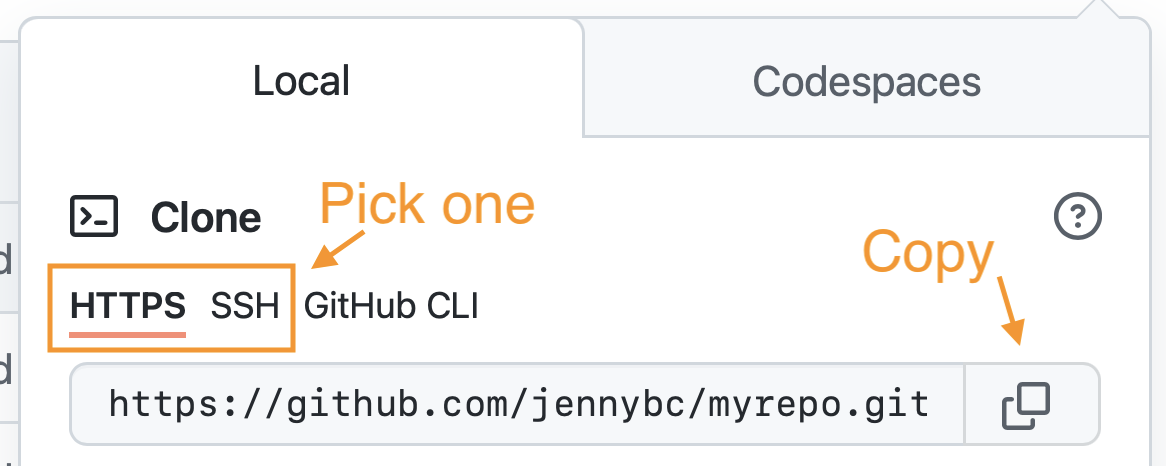
\includegraphics[width=0.6\linewidth]{img/github-https-or-ssh-url-annotated} \end{center}

\section{New RStudio Project via git clone}\label{git-clone-usethis-rstudio}

\begin{center}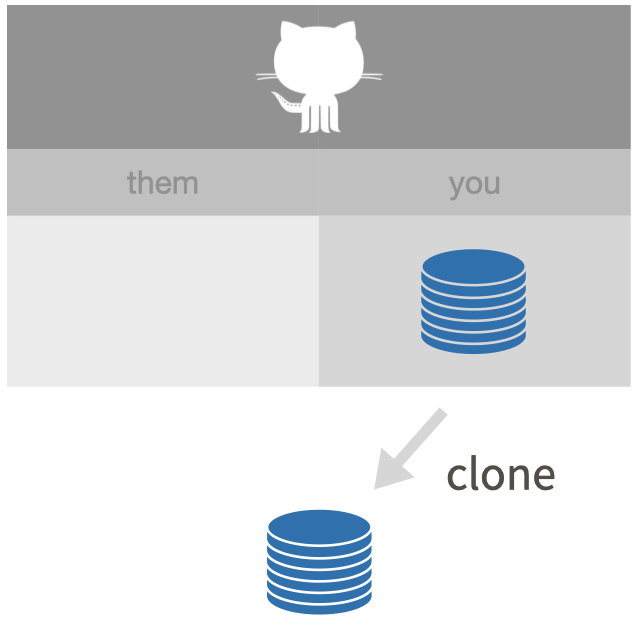
\includegraphics[width=0.6\linewidth]{img/new-project-github-first} \end{center}

I present two ways to do this:

\begin{itemize}
\tightlist
\item
  \texttt{usethis::create\_from\_github()}
\item
  Via the RStudio IDE
\end{itemize}

\emph{(Recall that we showed how to do this with command line Git in chapter \ref{push-pull-github}.)}

When you are cloning your own GitHub repository, the two methods are equivalent.
In other scenarios, especially fork-and-clone (chapter \ref{fork-and-clone}), I think \texttt{usethis::create\_from\_github()} is superior, because it does additional, recommended setup.

Pick \textbf{one} of these methods below.

\subsection{\texorpdfstring{\texttt{usethis::create\_from\_github()}}{usethis::create\_from\_github()}}\label{usethiscreate_from_github-1}

You can execute this command in any R session.
If you use RStudio, then do this in the R console of any RStudio instance.

\begin{Shaded}
\begin{Highlighting}[]
\NormalTok{usethis}\SpecialCharTok{::}\FunctionTok{create\_from\_github}\NormalTok{(}
  \StringTok{"https://github.com/YOU/YOUR\_REPO.git"}\NormalTok{,}
  \AttributeTok{destdir =} \StringTok{"\textasciitilde{}/path/to/where/you/want/the/local/repo/"}
\NormalTok{)}
\end{Highlighting}
\end{Shaded}

The first argument is \texttt{repo\_spec} and it accepts the GitHub repo specification in various forms.
In particular, you can use the URL we just copied from GitHub.

The \texttt{destdir} argument specifies the parent directory where you want the new folder (and local Git repo) to live.
If you don't specify \texttt{destdir}, usethis defaults to some very conspicuous place, like your desktop.
If you like to keep Git repos in a certain folder on your computer, you can personalize this default by setting the \texttt{usethis.destdir} option in your \texttt{.Rprofile}.

We're accepting the default behaviour of two other arguments, \texttt{rstudio} and \texttt{open}, because that's what most people will want.
For example, for an RStudio user, \texttt{create\_from\_github()} does this:

\begin{itemize}
\tightlist
\item
  Creates a new local directory in \texttt{destdir}, which is all of these things:

  \begin{itemize}
  \tightlist
  \item
    a directory or folder on your computer
  \item
    a Git repository, linked to a remote GitHub repository
  \item
    an RStudio Project
  \end{itemize}
\item
  Opens a new RStudio instance in the new Project
\item
  \textbf{In the absence of other constraints, I suggest that all of your R projects have exactly this set-up.}
\end{itemize}

\subsection{RStudio IDE}\label{rstudio-ide-1}

In RStudio, start a new Project:

\begin{itemize}
\tightlist
\item
  \emph{File \textgreater{} New Project \textgreater{} Version Control \textgreater{} Git}. In the ``repository URL'' paste
  the URL of your new GitHub repository. It will be something like this
  \texttt{https://github.com/jennybc/myrepo.git}.
\item
  Be intentional about where you create this Project.
\item
  I suggest you ``Open in new session''.
\item
  Click ``Create Project'' to create a new directory, which will be all of these things:

  \begin{itemize}
  \tightlist
  \item
    a directory or ``folder'' on your computer
  \item
    a Git repository, linked to a remote GitHub repository
  \item
    an RStudio Project
  \end{itemize}
\item
  \textbf{In the absence of other constraints, I suggest that all of your R projects have exactly this set-up.}
\end{itemize}

This should download the \texttt{README.md} file that we created on GitHub in the previous step.
Look in RStudio's file browser pane for the \texttt{README.md} file.

Behind the scenes, RStudio has done this for you:

\begin{Shaded}
\begin{Highlighting}[]
\NormalTok{git clone https://github.com/jennybc/myrepo.git}
\end{Highlighting}
\end{Shaded}

\section{Bring your existing project over}\label{bring-your-existing-project-over}

Using your favorite method of moving or copying files, copy the files that constitute your existing project into the directory for this new project.

In RStudio, consult the Git pane and the file browser.

\begin{itemize}
\tightlist
\item
  Are you seeing all the files? They should be here if your move/copy was successful.
\item
  Are they showing up in the Git pane with questions marks? They should be appearing as new untracked files.
\end{itemize}

\section{Stage and commit}\label{stage-and-commit}

Commit your files to this repo. How?

\begin{itemize}
\tightlist
\item
  Click the ``Git'' tab in upper right pane
\item
  Check the ``Staged'' box for all files that you want to commit.

  \begin{itemize}
  \tightlist
  \item
    Default: stage it.
  \item
    When to reconsider: this will all go to GitHub. Consider if that is
    appropriate for each file. \textbf{You can absolutely keep a file locally,
    without committing it to the Git repo and sending to GitHub}. Just let it
    sit there in your Git pane, without being staged. No harm will be done. If
    this is a long-term situation, list the file in \texttt{.gitignore}.
  \end{itemize}
\item
  If you're not already in the Git pop-up, click ``Commit''
\item
  Type a message in ``Commit message'', such as ``Init project XYZ''.
\item
  Click ``Commit''
\end{itemize}

\section{Push your local changes to GitHub}\label{push-your-local-changes-to-github-1}

Click the green ``Push'' button to send your local changes to GitHub.
RStudio will display something like:

\begin{Shaded}
\begin{Highlighting}[]
\NormalTok{\textgreater{}\textgreater{}\textgreater{} /usr/bin/git push origin HEAD:refs/heads/main}
\NormalTok{To https://github.com/jennybc/myrepo.git}
\NormalTok{   3a2171f..6d58539  HEAD {-}\textgreater{} main}
\end{Highlighting}
\end{Shaded}

\section{Confirm the local change propagated to the GitHub remote}\label{confirm-the-local-change-propagated-to-the-github-remote-3}

Go back to the browser.
I assume we're still viewing your new GitHub repo.

Refresh.

You should see all the project files you committed there.

If you click on ``commits,'' you should see one with the message you used, e.g.~``Init project XYZ''.

\section{The end}\label{the-end-1}

Now just ``lather, rinse, repeat''.
Do work somewhere: locally or on GitHub.
Commit it.
Push it or pull it, depending on where you did the work, but get local and remote ``synced up''.
Repeat.

Note that in general (and especially in future when collaborating with other developers) you will usually need to pull changes from the remote (GitHub) before pushing the local changes you have made.
For this reason, it's a good idea to try and get into the habit of pulling before you attempt to push.

\chapter{Existing project, GitHub last}\label{existing-github-last}

This an explicit workflow for connecting an existing local R project to GitHub, when for some reason you cannot or don't want to do a ``GitHub first'' workflow (see chapters \ref{new-github-first} and \ref{existing-github-first}).

When does this come up?
Example: it's an existing project that is already a Git repo with a history you care about.
Then you have to do this properly.

This may be less desirable for a novice because there are more opportunities to get confused and make a mistake.
But this workflow is not that hard, even with command line Git, and is even easier if you use conveniences from the \href{https://cran.r-project.org/package=usethis}{usethis} package or the RStudio IDE.
All of these are covered below.

\section{Prepare the local project}\label{prepare-the-local-project}

We assume you've got your existing R project isolated in a directory on your computer.
If that's not already true, make it so.
Create a directory and marshal all the existing data and R scripts there.
It doesn't really matter where you do this, but note where the project currently lives.

I encourage you to make this project into an RStudio project, although it is not absolutely required.
If you opt-out of this, the instructions using command line Git or usethis will still work for you, outside of RStudio.

\subsection{Make or verify an RStudio Project}\label{make-or-verify-an-rstudio-project}

If the project is not already an RStudio Project, make it so:

\begin{itemize}
\tightlist
\item
  Within RStudio you can do: \emph{File \textgreater{} New Project \textgreater{} Existing Directory} and, if you wish, ``Open in new session''.
\item
  Alternatively, from R, call \texttt{usethis::create\_project("path/to/your/project")}, substituting the path to your existing project directory.
\end{itemize}

If your project is already an RStudio Project, launch it.

\subsection{Make or verify a Git repo}\label{make-or-verify-a-git-repo}

You should be in RStudio now, in your project.

Is it already a Git repository?
The presence of the Git pane should tip you off.
If yes, you're done.

If not, you have several options:

\begin{itemize}
\tightlist
\item
  In the R Console, call \texttt{usethis::use\_git()}.
\item
  In RStudio, go to \emph{Tools \textgreater{} Project Options \ldots{} \textgreater{} Git/SVN}. Under ``Version control system'', select ``Git''. Confirm New Git Repository? Yes!
\item
  In the shell, with working directory set to the project's directory, do \texttt{git\ init}.
\end{itemize}

If you used usethis or RStudio to initialize the Git repo, the Project should re-launch in RStudio.
Do that yourself if you did \texttt{git\ init}.
RStudio should now have a Git pane.

\section{Stage and commit}\label{stage-and-commit-1}

If your local project was already a Git repo and was up-to-date, move on. Otherwise, you probably need to stage and commit.

\begin{itemize}
\tightlist
\item
  Click the ``Git'' tab in upper right pane
\item
  Check ``Staged'' box for all files you want to commit.

  \begin{itemize}
  \tightlist
  \item
    Default: stage everything
  \item
    When to do otherwise: this will all go to GitHub. So consider if that is
    appropriate for each file. \textbf{You can absolutely keep a file locally,
    without committing it to the Git repo and sending to GitHub}. Just let it
    sit there in your Git pane, without being staged. No harm will be done. If
    this is a long-term situation, list the file in \texttt{.gitignore}.
  \end{itemize}
\item
  If you're not already in the Git pop-up, click ``Commit''
\item
  Type a message in ``Commit message''.
\item
  Click ``Commit''
\end{itemize}

\section{Create and connect a GitHub repo}\label{create-and-connect-a-github-repo}

We'll show a few methods for creating a new GitHub repo and connecting it to your local repo.
Pick one.

\subsection{Create and connect a GitHub repo with usethis}\label{create-and-connect-a-github-repo-with-usethis}

To use usethis for this task, you must have configured a personal access token (PAT).
This will already by configured for anyone using HTTPS as their protocol, because they are already using the PAT to authenticate for other Git operations.
But if you are an SSH person, you will need to configure a PAT, which is explained in chapter \ref{https-pat}.
It is fine to have both a PAT and SSH keys.

In your project, in the R Console, call:

\begin{Shaded}
\begin{Highlighting}[]
\NormalTok{usethis}\SpecialCharTok{::}\FunctionTok{use\_github}\NormalTok{()}
\CommentTok{\#\textgreater{} ✓ Creating GitHub repository \textquotesingle{}jennybc/myrepo\textquotesingle{}}
\CommentTok{\#\textgreater{} ✓ Setting remote \textquotesingle{}origin\textquotesingle{} to \textquotesingle{}https://github.com/jennybc/myrepo.git\textquotesingle{}}
\CommentTok{\#\textgreater{} ✓ Pushing \textquotesingle{}main\textquotesingle{} branch to GitHub and setting \textquotesingle{}origin/main\textquotesingle{} as upstream branch}
\CommentTok{\#\textgreater{} ✓ Opening URL \textquotesingle{}https://github.com/jennybc/myrepo\textquotesingle{}}
\end{Highlighting}
\end{Shaded}

\begin{center}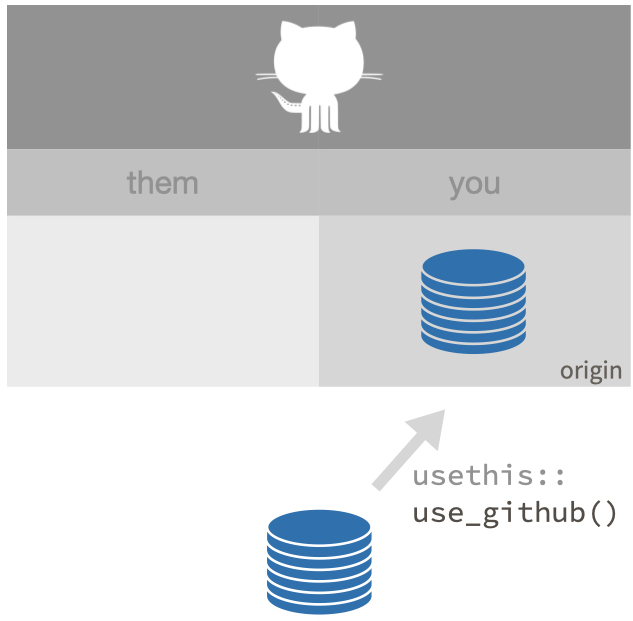
\includegraphics[width=0.6\linewidth]{img/use_github} \end{center}

\texttt{usethis::use\_github()} does the following:

\begin{itemize}
\tightlist
\item
  Creates a new repo on GitHub.
\item
  Configures that new repo as the \texttt{origin} remote for the local repo.
\item
  Sets up your local default branch (e.g.~\texttt{main}) to track same on \texttt{origin} and
  does an initial push.
\item
  Opens the new repo in your browser.
\end{itemize}

\subsection{Create and connect a GitHub repo without usethis}\label{create-and-connect-a-github-repo-without-usethis}

First, you need to create a new repo on GitHub.

Go to \url{https://github.com} and make sure you are logged in.

Near ``Repositories'', click the big green ``New'' button.
Or, if you are on your own profile page, click on ``Repositories'', then click the big green ``New'' button.

How to fill this in:

\begin{itemize}
\tightlist
\item
  Repository template: No template.
\item
  Repository name: Ideally this will be the name of your local project's directory (and RStudio Project). Why confuse yourself? But it must be a valid GitHub repo name, which means only letters, digits, \texttt{-}, \texttt{.}, or \texttt{\_} are allowed. For future projects, think about this in advance, i.e.~make sure each project's local name is also a valid GitHub repo name.
\item
  Description: ``Analysis of the stuff'' or any short description of the project. Write this for humans.
\item
  Public.
\item
  \textbf{DO NOT initialize this repository with anything}.
\end{itemize}

Click the big green button that says ``Create repository''.

Now click the big green button that says ``\textless\textgreater{} Code''.

Copy a clone URL to your clipboard.
If you're taking our default advice, copy the HTTPS URL.
But if you're opting for SSH, then make sure to copy the SSH URL.

\begin{center}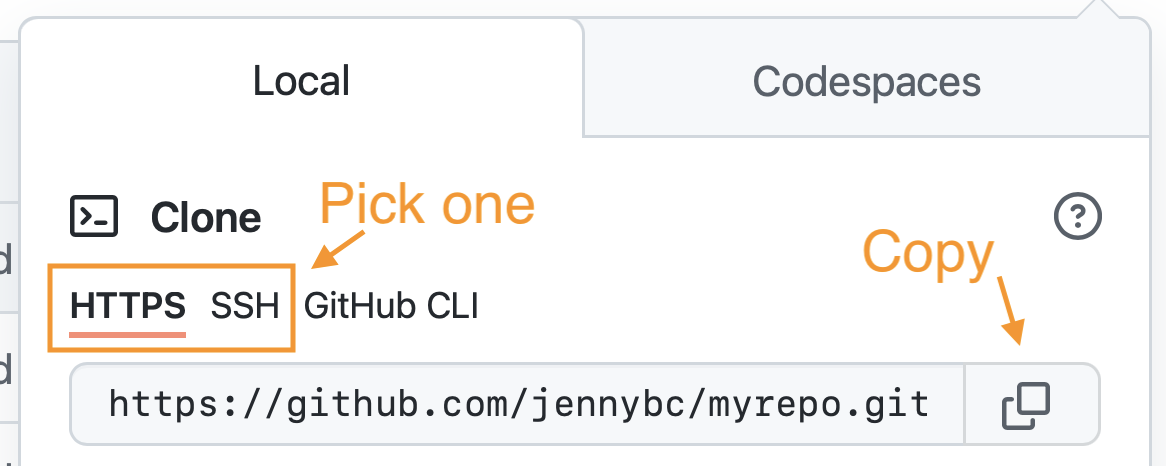
\includegraphics[width=0.6\linewidth]{img/github-https-or-ssh-url-annotated} \end{center}

\subsubsection{Connect local repo to GitHub repo with RStudio}\label{connect-local-repo-to-github-repo-with-rstudio}

Click on the ``two purple boxes and a white square'' in the Git pane.
Click ``Add remote''.
Paste the GitHub repo's URL here and pick a remote name, almost certainly \texttt{origin}.
Now ``Add''.

We should be back in the ``New Branch'' dialog (if not, click on the ``two purple boxes and a white square'' in the Git pane again).
I assume you're on the \texttt{main} branch and want it to track \texttt{main} on GitHub (or whatever default branch you are using).
Enter \texttt{main} as the branch name and make sure ``Sync branch with remote'' is checked.
Click ``Create'' (yes, even though the branch already exists).
In the next dialog, choose ``overwrite''.

\subsubsection{Connect local repo to GitHub repo with the command line}\label{connect-local-repo-to-github-repo-with-the-command-line}

In a shell, do this, substituting your URL:

\begin{Shaded}
\begin{Highlighting}[]
\NormalTok{git remote add origin https://github.com/jennybc/myrepo.git}
\end{Highlighting}
\end{Shaded}

Push and cement the tracking relationship between your local \texttt{main} branch and \texttt{main} on GitHub (or whatever your default branch is named):

\begin{Shaded}
\begin{Highlighting}[]
\NormalTok{git push {-}{-}set{-}upstream origin main}
\end{Highlighting}
\end{Shaded}

\section{Confirm the local files propagated to the GitHub remote}\label{confirm-the-local-files-propagated-to-the-github-remote}

Go back to the browser.
I assume we're still viewing your new GitHub repo.

Refresh.

You should see all the project files you committed there.

If this project already had a Git history, it should be reflected on GitHub.

\section{The end}\label{the-end-2}

Now just ``lather, rinse, repeat''.
Do work somewhere: locally or on GitHub.
Commit it.
Push it or pull it, depending on where you did the work, but get local and remote ``synced up''.
Repeat.

Note that in general (and especially in future when collaborating with other developers) you will usually need to pull changes from the remote (GitHub) before pushing the local changes you have made.
For this reason, it's a good idea to try and get into the habit of pulling before you attempt to push.

\chapter{Test drive R Markdown}\label{rmd-test-drive}

We will author an R Markdown document and render it to HTML.
We discuss how to keep the intermediate Markdown file, the figures, and what to commit to Git and push to GitHub.
If GitHub is the primary venue, we render directly to GitHub-flavored markdown and never create HTML.

Here is the official R Markdown documentation: \url{http://rmarkdown.rstudio.com}

\section{Hello World}\label{hello-world}

We'll practice with RStudio's boilerplate R Markdown document.

Launch RStudio in a Project that is a Git repo that is connected to a GitHub repo.

We are modelling ``walk before you run'' here.
It is best to increase complexity in small increments.
We test our system's ability to render the \href{http://en.wikipedia.org/wiki/\%22Hello,_world!\%22_program}{``hello world''} of R Markdown documents before we muddy the waters with our own, probably buggy, documents.

Do this: \emph{File \textgreater{} New File \textgreater{} R Markdown \ldots{}}

\begin{itemize}
\tightlist
\item
  Give it an informative title. This will appear in the document but does not
  necessarily have anything to do with the file's name. But the title and
  filename should be related! Why confuse yourself? The title is for human
  eyeballs, so it can contain spaces and punctuation. The filename is for humans
  and computers, so it should have similar words in it but no spaces and no
  punctuation.
\item
  Accept the default Author or edit if you wish.
\item
  Accept the default output format of HTML.
\item
  Click OK.
\end{itemize}

Save this document to a reasonable filename and location.
The filename should end in \texttt{.Rmd} or \texttt{.rmd}.
Save in the top-level of this RStudio project and Git repository, that is also current working directory.
Trust me on this and do this for a while.

You might want to commit at this point.
That will help you see exactly what's happening with your files, because this will appear as a ``diff'' in the Git pane.
Making change very visible is one of the big benefits of using Git.

Click on ``Knit HTML'' or do \emph{File \textgreater{} Knit Document}.
RStudio should display a preview of the resulting HTML.
Also look at the file browser.
You should see the original R Markdown document, i.e.~\texttt{foo.Rmd} AND the resulting HTML \texttt{foo.html}.

Congratulations, you've just made your first reproducible report with R Markdown.

This is another good time to commit changes.

\section{Push to GitHub}\label{push-to-github}

Push the current state to GitHub.

Go visit it in the browser.

Do you see the new files?
An R Markdown document and the associated HTML?
Visit both in the browser.
Verify this:

\begin{itemize}
\tightlist
\item
  Rmd is quite readable. But the output is obviously not there.
\item
  HTML is ugly.
\end{itemize}

\section{Output format}\label{output-format}

Do you really want HTML?
Do you only want HTML?
Are you absolutely sure?
If so, you can skip this step!

The magical process that turns your R Markdown to HTML is like so:

\begin{verbatim}
foo.Rmd --> foo.md --> foo.html
\end{verbatim}

Note the intermediate markdown, \texttt{foo.md}.
By default RStudio discards this, but you might want to hold on to that markdown file!

Why?
GitHub gives very special treatment to markdown files.
They are rendered in an almost HTML-like way.
This is great because it preserves all the charms of plain text, but gives you a pseudo-webpage for free when you visit the file in the browser.
In contrast, HTML is rendered as plain text on GitHub and you'll have to take special measures to see it the way you want.

In many cases, you \emph{only want the markdown}.
In that case, we switch the output format to \texttt{github\_document}.
This means rendering look like this:

\begin{verbatim}
foo.Rmd --> foo.md
\end{verbatim}

where \texttt{foo.md} is GitHub-flavored markdown.
If you still want the HTML \emph{but also the intermediate markdown}, there's a way to request that too.

This point we're making about the importance of \texttt{.md} files is why so many R packages have a \texttt{NEWS.md} file and \texttt{README.md}, often generated from \texttt{README.Rmd}.

\textbf{Output format} is one of the many things we can control in the YAML frontmatter of \texttt{.Rmd} documents, i.e.~the text at the top of your file between leading and trailing lines of \texttt{-\/-\/-}.

You can make some YAML changes via the RStudio IDE: click on the ``gear'' in the top bar of the source editor, near the ``Knit HTML'' button.
Select ``Output options'' and go to the Advanced tab and check ``Keep markdown source file.''
Your YAML should now look more like this:

\begin{Shaded}
\begin{Highlighting}[]
\PreprocessorTok{{-}{-}{-}}
\FunctionTok{title}\KeywordTok{:}\AttributeTok{ }\StringTok{"Something fascinating"}
\FunctionTok{author}\KeywordTok{:}\AttributeTok{ }\StringTok{"Jenny Bryan"}
\FunctionTok{date}\KeywordTok{:}\AttributeTok{ }\StringTok{"2024{-}09{-}04"}
\FunctionTok{output}\KeywordTok{:}
\AttributeTok{  }\FunctionTok{html\_document}\KeywordTok{:}
\AttributeTok{    }\FunctionTok{keep\_md}\KeywordTok{:}\AttributeTok{ }\CharTok{true}
\PreprocessorTok{{-}{-}{-}}
\end{Highlighting}
\end{Shaded}

You should have gained the line \texttt{keep\_md:\ true}.
You can also simply edit the file yourself to achieve this.
The IDE only exposes a small fraction of what's possible to configure in the YAML.

In fact, a hand-edit is necessary if you want to keep only markdown and get GitHub-flavored markdown.
In that case, make your YAML look like this:

\begin{Shaded}
\begin{Highlighting}[]
\PreprocessorTok{{-}{-}{-}}
\FunctionTok{title}\KeywordTok{:}\AttributeTok{ }\StringTok{"Something fascinating"}
\FunctionTok{author}\KeywordTok{:}\AttributeTok{ }\StringTok{"Jenny Bryan"}
\FunctionTok{date}\KeywordTok{:}\AttributeTok{ }\StringTok{"2024{-}09{-}04"}
\FunctionTok{output}\KeywordTok{:}\AttributeTok{ github\_document}
\PreprocessorTok{{-}{-}{-}}
\end{Highlighting}
\end{Shaded}

Save!

You might want to commit at this point.

Render via ``Knit HTML'' button.

Now revisit the file browser.
In addition to \texttt{foo.Rmd}, you should now see \texttt{foo.md}.
If there are R chunks that make figures, the usage of markdown output formats will also cause those figure files to be left behind in a sensibly named sub-directory, such as \texttt{foo\_files}.

If you commit and push \texttt{foo.md} and everything inside \texttt{foo\_files}, then anyone with permission to view your GitHub repo can see a decent-looking version of your report.

If your output format is \texttt{html\_document}, you should still see \texttt{foo.html}.
If your output format is \texttt{github\_document} and you see \texttt{foo.html}, that's leftover from earlier experiments.
Delete that.
It will only confuse you later.

You might want to commit here.

\section{Push to GitHub}\label{push-to-github-1}

Push the current state to GitHub.

Go visit it in the browser.

Do you see the modifications and new file(s)?
Your \texttt{.Rmd} should be modified, i.e.~you should see the changes you made to the YAML frontmatter.
And you should have gained, at least, the associated markdown file, \texttt{foo.md}.

\begin{itemize}
\tightlist
\item
  Visit the markdown file and compare to our previous HTML.
\item
  Do you see how the markdown is much more directly useful on GitHub?
  Internalize this lesson.
\end{itemize}

\section{Put your stamp on it}\label{put-your-stamp-on-it}

Select everything but the YAML frontmatter and \ldots{} delete it!

Write a single sentence.

Insert an empty R chunk, via the ``Chunk'' menu in upper right of source editor or with the corresponding keyboard shortcut.

\begin{verbatim}
```{r, eval=TRUE}
## insert your brilliant WORKING code here
```
\end{verbatim}

Insert 1 to 3 lines of functioning code that's relevant to you or the project where you're experimenting.
``Walk through'' and run those lines using the ``Run'' button or the corresponding keyboard shortcut.
You MUST make sure your code actually works!

Satisfied? Save!

You might want to commit here.

Now render the whole document via ``Knit HTML.'' Voilà!

You might want to commit here.
And push.
And admire your evolving progress on GitHub.

\section{Develop your report}\label{develop-your-report}

In this incremental manner, develop your report.
Add code to this chunk.
Refine it.
Add new chunks.
Go wild!
But keep running the code ``manually'' to make sure it actually works.

If the code doesn't work with you babysitting it, I can guarantee you it will fail, in a more spectacular and cryptic way, when run at arms-length via ``Knit HTML'' or \texttt{rmarkdown::render()}.

Clean out your workspace and restart R and re-run everything periodically, if things get weird.
There are lots of chunk menu items and keyboard shortcuts to accelerate this workflow.
Render the whole document often to catch errors when they're easy to pinpoint and fix.
Save often and commit every time you reach a point that you'd like as a ``fall back'' position.

You'll develop your own mojo soon, but this should give you your first successful R Markdown experience.

\section{Publish your report}\label{publish-your-report}

If you've been making HTML, you can put that up on the web somewhere, email it to your collaborator, whatever.

No matter what, technically you can publish this report merely by pushing a rendered version to GitHub.
However, certain practices make this effort at publishing more satisfying for your audience.

Here are two behaviors I find very frustrating:

\begin{itemize}
\tightlist
\item
  ``Here is my code. Behold.'' This is when someone only pushes their source, i.e.
  R Markdown or R code, AND they really want other people to appreciate their
  ``product''. The implicit assumption is that the target audience will download
  all of the data and code and execute it locally.
\item
  ``Here is my HTML. Behold.'' This is when someone accepts the default HTML-only
  output. Remember, HTML files on GitHub are not readable by humans. Therefore,
  the implicit assumption is that the target audience will download the repo
  and point their browser at this HTML file, in order to see it.
  HTML on GitHub? It's not readable by humans.
\end{itemize}

Sometimes it's just very unrealistic to expect your audience to take the extra steps described above.
Often, with a very small change on your end, you can create an artefact on GitHub that your target audience can immediately appreciate.

Creating, committing, and pushing markdown (i.e., \texttt{.md} files) is a very functional, lighweight publishing strategy.
Use \texttt{output:\ github\_document} or, if output is \texttt{html\_document}, add \texttt{keep\_md:\ true}.
In both cases, it is critical to also commit and push everything inside \texttt{foo\_files}, i.e.~any figures that have been created.
Now people can visit and consume your work on GitHub, like any other webpage.

This is (sort of) another example of a generally worthy principle, which is keeping things machine- and human-readable, whenever possible.
By making \texttt{foo.Rmd} available, others can see and run your \textbf{actual code}.
By also sharing \texttt{foo.md} and/or \texttt{foo.html}, others can casually browse your end product and decide if they want to obtain and run the code.

\section{HTML on GitHub}\label{html-on-github}

HTML files, such as \texttt{foo.html}, are not immediately useful on GitHub (though your local versions are easily viewable).
Visit one and you'll see the raw HTML.
Yuck.
But there are ways to get a preview: such as \url{http://htmlpreview.github.io}. Expect much pain with HTML files inside private repos (hence the recommendations above to emphasize markdown).
When it becomes vital for the whole world to see proper HTML in its full glory, it's time to use a more sophisticated web publishing strategy.

I have more \hyperref[workflows-browsability]{general ideas} about how to make a GitHub repo function as a website.

\section{Troubleshooting}\label{rmd-troubleshooting}

\textbf{Make sure RStudio and the rmarkdown package (and its dependencies) are up-to-date.}
In case of catastrophic failure to render the boilerplate R Markdown document, consider that your software may be too old.
Details on the system used to render this document and how to check your setup:

\begin{itemize}
\tightlist
\item
  rmarkdown version 2.28.
  Use \texttt{packageVersion("rmarkdown")} to check yours.
\item
  R version 4.4.1 (2024-06-14). Use \texttt{R.version.string} to check yours.
\item
  RStudio IDE 2021.9.0.341 (``Ghost Orchid'' Preview).
  Use \emph{RStudio \textgreater{} About RStudio} or \texttt{RStudio.Version()\$version} to check yours.
\end{itemize}

\textbf{Get rid of your \texttt{.Rprofile}}, at least temporarily.
I have found that a ``mature'' \texttt{.Rprofile} that has accumulated haphazardly over the years can cause trouble.
Specifically, if you've got anything in there relating to knitr, markdown, rmarkdown, or RStudio itself, it may be preventing the installation or usage of the most recent goodies.
Comment the whole file out or rename it to something else and relaunch or even re-install RStudio.

\textbf{``I have ignored your advice and dumped a bunch of code in at once. Now my Rmd does not render.''}
If you can't figure out what's wrong by reading the error messages, pick one:

\begin{itemize}
\tightlist
\item
  Back out of these changes, get back to a functional state (possibly with no
  code), and restore them gradually. Run your code interactively to make sure it
  works. Render the entire document frequently. Commit after each successful
  addition! When you re-introduce the broken code, now it will be part of a
  small change and the root problem will be much easier to pinpoint and fix.
\item
  Tell knitr to soldier on, even in the presence of errors. Some problems are
  easier to diagnose if you can execute specific R statements during rendering
  and leave more evidence behind for forensic examination.

  \begin{itemize}
  \item
    Insert this chunk near the top of your \texttt{.Rmd} document:

\begin{verbatim}
```{r setup, include = FALSE, cache = FALSE}
knitr::opts_chunk$set(error = TRUE)
```
\end{verbatim}
  \item
    If it's undesirable to globally accept errors, you can still specify
    \texttt{error\ =\ TRUE} for a specific chunk like so:

\begin{verbatim}
```{r wing-and-a-prayer, error = TRUE}
## your sketchy code goes here ;)
```
\end{verbatim}
  \end{itemize}
\item
  Adapt the \href{http://webchick.net/node/99}{``git bisect'' strategy}:

  \begin{itemize}
  \tightlist
  \item
    Put \texttt{knitr::knit\_exit()} somewhere early in your \texttt{.Rmd} document, either in
    inline R code or in a chunk.
    Keep moving it earlier until things work.
    Now move it down in the document.
    Eventually you'll be able to narrow down the location of your broken code
    well enough to find the line(s) and fix it.
  \end{itemize}
\end{itemize}

\textbf{Check your working directory.}
It's going to break your heart as you learn how often your mistakes are really mundane and basic.
Ask me how I know.
When things go wrong consider:

\begin{itemize}
\tightlist
\item
  What is the working directory?
\item
  Is that file I want to read/write actually where I think it is?
\end{itemize}

Drop these commands into R chunks to check the above:

\begin{itemize}
\tightlist
\item
  \texttt{getwd()} will display working directory at \textbf{run time}.
  If you monkeyed around with working directory with, e.g., the mouse, maybe
  it's set to one place for your interactive development and another when
  ``Knit HTML'' takes over?
\item
  \texttt{list.files()} will list the files in working directory.
  Is the file you want even there?
\end{itemize}

\textbf{Don't try to change working directory within an R Markdown document}.
Just don't.
See \href{https://yihui.name/knitr/faq/}{knitr FAQ \#5}.
That is all.

\textbf{Don't be in a hurry to create a complicated sub-directory structure.}
RStudio/knitr/rmarkdown (which bring you the ``Knit HTML'' button) are rather opinionated about the working directory being set to the \texttt{.Rmd} file's location and about all files living together in one big happy directory.
This can all be worked around.
For example, I \href{https://github.com/jennybc/here_here\#readme}{recommend the here package} for building file paths, once you require sub-directories.
But don't do this until you really need it.

\chapter{Render an R script}\label{r-test-drive}

An under-appreciated fact is that much of what you can do with R Markdown, you can also do with an R script.

If you're in analysis mode and want a report as a side effect, write an R script.
If you're writing a report with a lot of R code in it, write \texttt{.Rmd}.
In either case, render to markdown and/or HTML to communicate with other human beings.

\begin{itemize}
\tightlist
\item
  In R markdown, prose is top-level and code is tucked into chunks.
\item
  In R scripts, code is top-level and prose is tucked into comments.
  You will use \texttt{\#\textquotesingle{}} to request that certain comments appear as top-level prose
  in the rendered output.
\end{itemize}

You will continue to specify things like the output format via YAML at the top of the file.
This will need to be commented with \texttt{\#\textquotesingle{}}.

\section{Morph R Markdown into a renderable R script}\label{morph-r-markdown-into-a-renderable-r-script}

Get yourself a working R Markdown file, such as the one you made in your \hyperref[rmd-test-drive]{Rmd test drive}.
Or use the boilerplate \texttt{.Rmd} document RStudio makes with \emph{File \textgreater{} New File \textgreater{} R Markdown \ldots{}}.

Save the file as \texttt{foo.R}, as opposed to \texttt{foo.Rmd}.
Yes, for a brief moment, you will have R Markdown saved as an R script, but that won't be true for long.

Transform the R markdown to R:

\begin{itemize}
\item
  Anything that's not R code?
  Like the YAML and the prose?
  Protect it with roxygen-style comments: start each line with \texttt{\#\textquotesingle{}}.
\item
  Anything that is R code?
  Let it exist ``as is'' as top-level code.
  That means you'll need to change the syntax of R chunk headers like so:

  Before: \texttt{\textasciigrave{}\textasciigrave{}\textasciigrave{}\{r\ setup,\ include\ =\ FALSE\}}\\
  After: \texttt{\#+\ r\ setup,\ include\ =\ FALSE}

  Replace the leading backticks and opening curly brace with \texttt{\#+}.\\
  Delete the trailing curly brace.\\
  Delete the 3 backticks that end each chunk.
\end{itemize}

Render the R script through one of these methods:

\begin{itemize}
\tightlist
\item
  Click on the ``notebook'' icon in RStudio to ``Compile Report''.
\item
  In RStudio, do \emph{File \textgreater{} Knit Document}.
\item
  In R, do \texttt{rmarkdown::render("foo.R")}.
\end{itemize}

You'll get a markdown and/or HTML report, just as with R Markdown.

If you're having trouble making all the necessary changes and you're frustrated, see below for an example you can copy and paste.

All the workflow tips from the \hyperref[rmd-test-drive]{Rmd test drive} apply here:
when you script an analysis, render it to markdown, commit the \texttt{.R}, the \texttt{.md}, any associated figures, and push to GitHub.
Collaborators can see your code, but also browse around the results without having to download and execute the code.
This makes the current state of your analysis accessible to someone who does not even run R or who wants to take a quick look at things from a cell phone or while on vacation.

\section{Write a render-ready R script}\label{write-a-render-ready-r-script}

Instead of morphing an R Markdown file, let's create a render-ready R script directly.

Create a new R script and copy/paste this code into it.

\begin{Shaded}
\begin{Highlighting}[]
\CommentTok{\#\textquotesingle{} Here\textquotesingle{}s some prose in a very special comment. Let\textquotesingle{}s summarize the built{-}in}
\CommentTok{\#\textquotesingle{} dataset \textasciigrave{}VADeaths\textasciigrave{}.}
\CommentTok{\# here is a regular code comment, that will remain as such}
\FunctionTok{summary}\NormalTok{(VADeaths)}

\CommentTok{\#\textquotesingle{} Here\textquotesingle{}s some more prose. I can use usual markdown syntax to make things}
\CommentTok{\#\textquotesingle{} **bold** or *italics*. Let\textquotesingle{}s use an example from the \textasciigrave{}dotchart()\textasciigrave{} help to}
\CommentTok{\#\textquotesingle{} make a Cleveland dot plot from the \textasciigrave{}VADeaths\textasciigrave{} data. I even bother to name}
\CommentTok{\#\textquotesingle{} this chunk, so the resulting PNG has a decent name.}
\CommentTok{\#+ dotchart}
\FunctionTok{dotchart}\NormalTok{(VADeaths, }\AttributeTok{main =} \StringTok{"Death Rates in Virginia {-} 1940"}\NormalTok{)}
\end{Highlighting}
\end{Shaded}

Render the R script through one of these methods:

\begin{itemize}
\tightlist
\item
  Click on the ``notebook'' icon in RStudio to ``Compile Report''.
\item
  In RStudio, do \emph{File \textgreater{} Knit Document}.
\item
  In R, do \texttt{rmarkdown::render("YOURSCRIPT.R")}.
\end{itemize}

Revel in your attractive looking report with almost zero effort!
Seriously, all you had to do was think about when to use special comments \texttt{\#\textquotesingle{}} in order to promote that to nicely rendered text.

Drawing on the workflow tips in \hyperref[rmd-test-drive]{Rmd test drive}, let's add some YAML frontmatter, properly commented with \texttt{\#\textquotesingle{}}, and request \texttt{github\_document} as the output format.
Here's the whole script again:

\begin{Shaded}
\begin{Highlighting}[]
\CommentTok{\#\textquotesingle{} {-}{-}{-}}
\CommentTok{\#\textquotesingle{} title: "R scripts can be rendered!"}
\CommentTok{\#\textquotesingle{} output: github\_document}
\CommentTok{\#\textquotesingle{} {-}{-}{-}}
\CommentTok{\#\textquotesingle{}}
\CommentTok{\#\textquotesingle{} Here\textquotesingle{}s some prose in a very special comment. Let\textquotesingle{}s summarize the built{-}in}
\CommentTok{\#\textquotesingle{} dataset \textasciigrave{}VADeaths\textasciigrave{}.}
\CommentTok{\# here is a regular code comment, that will remain as such}
\FunctionTok{summary}\NormalTok{(VADeaths)}

\CommentTok{\#\textquotesingle{} Here\textquotesingle{}s some more prose. I can use usual markdown syntax to make things}
\CommentTok{\#\textquotesingle{} **bold** or *italics*. Let\textquotesingle{}s use an example from the \textasciigrave{}dotchart()\textasciigrave{} help to}
\CommentTok{\#\textquotesingle{} make a Cleveland dot plot from the \textasciigrave{}VADeaths\textasciigrave{} data. I even bother to name}
\CommentTok{\#\textquotesingle{} this chunk, so the resulting PNG has a decent name.}
\CommentTok{\#+ dotchart}
\FunctionTok{dotchart}\NormalTok{(VADeaths, }\AttributeTok{main =} \StringTok{"Death Rates in Virginia {-} 1940"}\NormalTok{)}
\end{Highlighting}
\end{Shaded}

Behind the scenes here we have used \texttt{rmarkdown::render()} to render this script and you can go \href{https://github.com/jennybc/happy-git-with-r/blob/master/render-r-script-demo.md}{visit it on GitHub}.

\part{Git fundamentals}\label{part-git-fundamentals}

\chapter*{Some Git basics}\label{git-intro}
\addcontentsline{toc}{chapter}{Some Git basics}

We've told you shockingly little about Git so far! This is by design.

We find that actual usage, in the course of your work, is the most effective way to build up a useful mental model for Git. In live workshops, we strive to introduce the most important basic ideas in the context of our guided activities. Self-learners can achieve the same by working through the ``batteries included'' guides earlier in the previous sections.

However, building on this early success, now is the perfect time to explicitly define some Git vocabulary. We also want to help you link Git concepts to data science tasks and projects.

This part collects anything we've written about core Git concepts. It is a work in progress and is conceived as a complement to the many excellent \hyperref[resources]{external resources for Git}, which we have no desire to re-invent.

\chapter{Repo, commit, diff, tag}\label{git-basics}

\section{Repos or repositories}\label{repos-or-repositories}

Git is a version control system whose original purpose was to help groups of
developers work collaboratively on big software projects. Git manages the
evolution of a set of files -- called a \textbf{repository} or \textbf{repo} -- in a highly structured way. Historically, these files would have consisted of source code and the instructions for how to build an application from its source.

Git has been re-purposed by the data science community (\citeproc{ref-Ram2013}{Ram 2013}; \citeproc{ref-git-for-humans}{Bartlett 2016}; \citeproc{ref-ten-simple-rules-git}{Perez-Riverol et al. 2016}). We use it to manage the motley collection of files that make up typical data analytical projects, which consist of data, figures, reports, and, yes, some source code.

For new or existing projects, we recommend that you:

\begin{itemize}
\tightlist
\item
  Dedicate a local directory or folder to it.
\item
  Make it an RStudio Project. \emph{Optional but recommended; obviously only applies to projects involving R and users of RStudio.}
\item
  Make it a Git repository.
\end{itemize}

This setup happens once per project and can happen at project inception or at any later point. Chances are your existing projects each already live in a dedicated directory. Making such a directory an RStudio Project and Git repository boils down to allowing those applications to leave notes for themselves in hidden files or directories. The project is still a regular directory on your computer, that you can locate, name, move, and generally interact with as you wish. You don't have to handle it with special gloves!

The daily workflow is probably not dramatically different from what you do currently. You work in the usual way, writing R scripts or authoring reports in LaTeX or R Markdown. But instead of only \emph{saving} individual files, periodically you make a \textbf{commit}, which takes a snapshot of all the files in the entire project. If you have ever versioned a file \href{http://www.phdcomics.com/comics/archive.php?comicid=1531}{by adding your initials or the date}, you have effectively made a commit, albeit only for a single file. It is a version that is significant to you and that you might want to inspect or revert to later. Periodically, you push commits to GitHub. This is like sharing a document with colleagues on DropBox or sending it out as an email attachment. By pushing to GitHub, you make your work and all your accumulated progress accessible to others.

This is a moderate change to your normal, daily workflow. It feels weird at first, but quickly becomes second nature. In \href{http://stat545.com}{STAT 545} students are required to submit all coursework via GitHub, starting in week one. Most have never seen Git before and do not identify as programmers. It is a major topic in class and office hours for the first two weeks. Then we practically never discuss it again.

\section{Commits, diffs, and tags}\label{commits-diffs-and-tags}

We now connect the fundamental concepts of Git to the data science workflow:

\begin{itemize}
\tightlist
\item
  repository
\item
  commit
\item
  diff
\end{itemize}

Recall that a repository or repo is just a directory of files that Git manages holistically. A commit functions like a snapshot of all the files in the repo, at a specific moment. Under the hood, that is not exactly how Git implements things. Although mental models don't have to be accurate in order to be useful, in this case it helps to align the two.

\begin{figure}
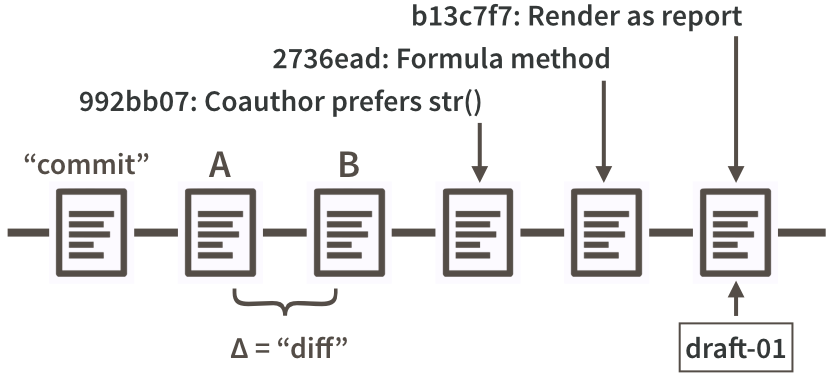
\includegraphics[width=1\linewidth]{img/commit-diff-sha-tag} \caption{\label{fig:commit-diff-sha-tag}Partial commit history for our iris example, highlighting diffs, commit messages, SHAs, and tags.}\label{fig:commit-diff-sha-tag}
\end{figure}

Figure \ref{fig:commit-diff-sha-tag} is a look at a fictional analysis of the iris data, focusing on the evolution of a script, \texttt{iris.R}. Consider version A of this file and a modified version, version B. Assume that version A was part of one Git commit and version B was part of the next commit. The set of differences between A and B is called a ``diff'' and Git users contemplate diffs a lot. Diff inspection is how you re-explain to yourself how version A differs from version B. Diff inspection is not limited to adjacent commits. You can inspect the diffs between any two commits.

In fact, Git's notion of any specific version of \texttt{iris.R} is as an accumulation of diffs. If you go back far enough, you find the commit where the file was created in the first place. Every later version is stored by Git as that initial version, plus all the intervening diffs in the history that affect the file. We'll set these internal details aside now, but understanding the importance of these deltas will make Git's operations less baffling in the long run.

So, by looking at diffs, it's easy to see how two snapshots differ, but what about the why?

Every time you make a commit you must also write a short \textbf{commit message}. Ideally, this conveys the motivation for the change. Remember, the diff will show the content. When you revisit a project after a break or need to digest recent changes made by a colleague, looking at the \textbf{history}, by reading commit messages and skimming through diffs, is an extremely efficient way to get up to speed. Figure \ref{fig:commit-diff-sha-tag} shows the messages associated with the last three commits.

Every commit needs some sort of nickname, so you can identify it. Git does this automatically, assigning each commit what is called a SHA, a seemingly random string of 40 letters and numbers (it is not, in fact, random but is a SHA-1 checksum hash of the commit). Though you will be exposed to these, you don't have to handle them directly very often and, when you do, usually the first 7 characters suffice. The commit messages in Figure \ref{fig:commit-diff-sha-tag} are prefixed by such truncated SHAs. You can also designate certain snapshots as special with a \textbf{tag}, which is a name of your choosing. In a software project, it is typical to tag a release with its version, e.g., ``v1.0.3''. For a manuscript or analytical project, you might tag the version submitted to a journal or transmitted to external collaborators. Figure \ref{fig:commit-diff-sha-tag} shows a tag, ``draft-01'', associated with the last commit.

\chapter{Git commands}\label{git-commands}

A collection of some of the Git commands that have been largely going on under the hood.
We've emphasized early workflows that are possible in RStudio.
But all of this and much more can be done from the command line.
This list is here mostly so we can consult it during live workshops if needed.

\emph{Unless you use the \href{https://developer.github.com/v3/}{GitHub API}, most of the GitHub bits really have to be done from the browser.}

New local git repo from a repo on GitHub:

\begin{Shaded}
\begin{Highlighting}[]
\NormalTok{git clone https://github.com/jennybc/happy{-}git{-}with{-}r.git}
\end{Highlighting}
\end{Shaded}

Check the remote was cloned successfully:

\begin{Shaded}
\begin{Highlighting}[]
\NormalTok{git remote {-}{-}verbose}
\end{Highlighting}
\end{Shaded}

Stage local changes, commit:

\begin{Shaded}
\begin{Highlighting}[]
\NormalTok{git add foo.txt}
\NormalTok{git commit {-}{-}message "A commit message"}
\end{Highlighting}
\end{Shaded}

Check on the state of the Git world:

\begin{Shaded}
\begin{Highlighting}[]
\NormalTok{git status}
\NormalTok{git log}
\NormalTok{git log {-}{-}oneline}
\end{Highlighting}
\end{Shaded}

Compare versions:

\begin{Shaded}
\begin{Highlighting}[]
\NormalTok{git diff}
\end{Highlighting}
\end{Shaded}

Add a remote to existing local repo:

\begin{Shaded}
\begin{Highlighting}[]
\NormalTok{git remote add origin https://github.com/jennybc/happy{-}git{-}with{-}r}
\NormalTok{git remote {-}{-}verbose}
\NormalTok{git remote show origin}
\end{Highlighting}
\end{Shaded}

Push local \texttt{main} to GitHub \texttt{main} and have local \texttt{main} track \texttt{main} on GitHub:

\begin{Shaded}
\begin{Highlighting}[]
\NormalTok{git push {-}{-}set{-}upstream origin main}
\NormalTok{\# shorter form}
\NormalTok{git push {-}u origin main}
\NormalTok{\# you only need to set upstream tracking once!}
\end{Highlighting}
\end{Shaded}

Regular push:

\begin{Shaded}
\begin{Highlighting}[]
\NormalTok{git push }
\NormalTok{\# the above usually implies (and certainly does in our tutorial)}
\NormalTok{git push origin main}
\NormalTok{\# git push [remote{-}name] [branch{-}name]}
\end{Highlighting}
\end{Shaded}

Pull commits from GitHub:

\begin{Shaded}
\begin{Highlighting}[]
\NormalTok{git pull}
\end{Highlighting}
\end{Shaded}

Pull commits and don't let it put you in a merge conflict pickle:

\begin{Shaded}
\begin{Highlighting}[]
\NormalTok{git pull {-}{-}ff{-}only}
\end{Highlighting}
\end{Shaded}

Fetch commits

\begin{Shaded}
\begin{Highlighting}[]
\NormalTok{git fetch}
\end{Highlighting}
\end{Shaded}

Switch to a branch

\begin{Shaded}
\begin{Highlighting}[]
\NormalTok{git checkout [branch{-}name]}
\end{Highlighting}
\end{Shaded}

Checking remote and branch tracking

\begin{Shaded}
\begin{Highlighting}[]
\NormalTok{git remote {-}v}
\NormalTok{git remote show origin}
\NormalTok{git branch {-}vv}
\end{Highlighting}
\end{Shaded}

\chapter{Branches}\label{git-branches}

Branching means that you take a detour from the main stream of development and
do work without changing the main stream.
It allows one or many people to work in parallel without overwriting each other's work.
It allows a someone working solo to work incrementally on an experimental idea, without jeopardizing the state of the main product.

Branching in Git is very lightweight, which means creating a branch and
switching between branches is nearly instantaneous.
This means Git encourages workflows which create small branches for exploration or new features, often merging them back together quickly.

\section{Create a new branch}\label{create-a-new-branch}

You can create a new branch with \texttt{git\ branch}, then checkout the branch with \texttt{git\ checkout}.
To distinguish it from the main stream of development, presumably on \texttt{main}, we'll call this a ``feature branch''.

\begin{Shaded}
\begin{Highlighting}[]
\NormalTok{git branch issue{-}5}
\NormalTok{git checkout issue{-}5}
\end{Highlighting}
\end{Shaded}

You can also use the shortcut \texttt{git\ checkout\ -b\ issue-5} to create and checkout the branch all at once.

Once you have switched to a branch, you can commit to it as usual.

\section{Switching branches}\label{switching-branches}

You use \texttt{git\ checkout} to switch between branches.

But what do you do if you are working on a branch and need to switch,
but the work on the current branch is not complete?
One option is the \href{https://git-scm.com/book/en/v2/ch00/_git_stashing}{Git stash}, but generally a better option is to safeguard the current state with a temporary commit.
Here I use ``WIP'' as the commit message to indicate work in progress.

\begin{Shaded}
\begin{Highlighting}[]
\NormalTok{git commit {-}{-}all {-}m "WIP"}
\NormalTok{git checkout main}
\end{Highlighting}
\end{Shaded}

Then when you come back to the branch and continue your work, you
need to undo the temporary commit by \hyperref[reset]{resetting} your state.
Specifically, we want a mixed reset.
This is ``working directory safe'', i.e.~it does not affect the state of any files.
But it does peel off the temporary WIP commit.
Below, the reference \texttt{HEAD\^{}} says to roll the commit state back to the parent of the current commit (\texttt{HEAD}).

\begin{Shaded}
\begin{Highlighting}[]
\NormalTok{git checkout issue{-}5}
\NormalTok{git reset HEAD\^{}}
\end{Highlighting}
\end{Shaded}

If this is difficult to remember, or to roll the commit state back to a different previous state, the reference can also be given as the SHA of a specific commit, which you can see via \texttt{git\ log}.
This is where I think a graphical Git client can be invaluable, as you can generally right click on the target commit, then select the desired type of reset (e.g., soft, mixed, or hard).
This is exactly the type of intermediate-to-advanced Git usage that often feels more approachable in a graphical client.

\section{Merging a branch}\label{merging-a-branch}

Once you have done your work and committed it to the feature branch, you can switch back to \texttt{main} and merge the feature branch.

\begin{Shaded}
\begin{Highlighting}[]
\NormalTok{git checkout main}
\NormalTok{git merge issue{-}5}
\end{Highlighting}
\end{Shaded}

\section{Dealing with conflicts}\label{dealing-with-conflicts}

Most of the time, the merge will go smoothly.
However if both the branches you are merging changed the same part of the same file you will get a merge conflict.

\begin{Shaded}
\begin{Highlighting}[]
\NormalTok{git merge issue{-}5}
\NormalTok{\# Auto{-}merging index.html}
\NormalTok{\# CONFLICT (content): Merge conflict in index.html}
\NormalTok{\# Automatic merge failed; fix conflicts and then commit the result.}
\end{Highlighting}
\end{Shaded}

The first thing to do is \textbf{NOT PANIC}.
Merge conflicts are not the end of the world and most are relatively small and straightforward to resolve.

The first step to solving a merge conflict is determining which files are in
conflict, which you can do with \texttt{git\ status}:

\begin{Shaded}
\begin{Highlighting}[]
\NormalTok{git status}
\NormalTok{\# On branch main}
\NormalTok{\# You have unmerged paths.}
\NormalTok{\#   (fix conflicts and run "git commit")}
\NormalTok{\# }
\NormalTok{\# Unmerged paths:}
\NormalTok{\#   (use "git add \textless{}file\textgreater{}..." to mark resolution)}
\NormalTok{\# }
\NormalTok{\#     both modified:      index.html}
\NormalTok{\# }
\NormalTok{\# no changes added to commit (use "git add" and/or "git commit {-}a")}
\end{Highlighting}
\end{Shaded}

So this shows only \texttt{index.html} is unmerged and needs to be resolved.
We can then open the file to see what lines are in conflict.

\begin{Shaded}
\begin{Highlighting}[]
\ErrorTok{\textless{}\textless{}\textless{}\textless{}\textless{}\textless{}\textless{}}\NormalTok{ HEAD:index.html}
\DataTypeTok{\textless{}}\KeywordTok{div}\OtherTok{ id}\OperatorTok{=}\StringTok{"footer"}\DataTypeTok{\textgreater{}}\NormalTok{contact : email.support@github.com}\DataTypeTok{\textless{}/}\KeywordTok{div}\DataTypeTok{\textgreater{}}
\NormalTok{=======}
\DataTypeTok{\textless{}}\KeywordTok{div}\OtherTok{ id}\OperatorTok{=}\StringTok{"footer"}\DataTypeTok{\textgreater{}}
\NormalTok{ please contact us at support@github.com}
\DataTypeTok{\textless{}/}\KeywordTok{div}\DataTypeTok{\textgreater{}}
\NormalTok{\textgreater{}\textgreater{}\textgreater{}\textgreater{}\textgreater{}\textgreater{}\textgreater{} issue{-}5:index.html}
\end{Highlighting}
\end{Shaded}

In this conflict, the lines between \texttt{\textless{}\textless{}\textless{}\textless{}\textless{}\textless{}\ HEAD:index.html} and \texttt{======} are
the content from the branch you are currently on.
The lines between \texttt{=======} and \texttt{\textgreater{}\textgreater{}\textgreater{}\textgreater{}\textgreater{}\textgreater{}\textgreater{}\ issue-5:index.html} are from the feature branch we are merging.

To resolve the conflict, edit this section until it reflects the state you want in the merged result.
Pick one version or the other or create a hybrid.
Also remove the conflict markers \texttt{\textless{}\textless{}\textless{}\textless{}\textless{}\textless{}}, \texttt{======} and \texttt{\textgreater{}\textgreater{}\textgreater{}\textgreater{}\textgreater{}\textgreater{}}.

\begin{Shaded}
\begin{Highlighting}[]
\DataTypeTok{\textless{}}\KeywordTok{div}\OtherTok{ id}\OperatorTok{=}\StringTok{"footer"}\DataTypeTok{\textgreater{}}
\NormalTok{please contact us at email.support@github.com}
\DataTypeTok{\textless{}/}\KeywordTok{div}\DataTypeTok{\textgreater{}}
\end{Highlighting}
\end{Shaded}

Now run \texttt{git\ add\ index.html} and \texttt{git\ commit} to finalize the merge.
CONFLICTS RESOLVED.

\subsection{Bailing out}\label{bailing-out}

If, during the merge, you get confused about the state of things or make a
mistake, use \texttt{git\ merge\ -\/-abort} to abort the merge and go back to the state
prior to running \texttt{git\ merge}.
Then you can try to complete the merge again.

Git Basic Branching and Merging:

\url{https://git-scm.com/book/en/v2/Git-Branching-Basic-Branching-and-Merging}

\chapter{Remotes}\label{git-remotes}

Remote repositories are versions of your project that are hosted on the
Internet or another network.
A single project can have 1, 2, or even hundreds of remotes.
You pull others' changes from remotes and push your changes to remotes.

\section{Listing what remotes exist}\label{listing-what-remotes-exist}

\texttt{git\ remote} lists the names of available remotes, but usually it is more
useful to see what URLs each note corresponds to (with \texttt{-v}).

\#\texttt{\{bash\}\ \#git\ remote\ -v\ \#}

\section{Adding a new remote}\label{adding-a-new-remote}

\texttt{git\ clone} automatically adds a new remote, so often you do not need to do
this manually initially.
However, after the initial clone, it is often useful to add additional remotes.

Use \texttt{git\ remote\ add} to add a new remote:

\begin{Shaded}
\begin{Highlighting}[]
\NormalTok{git remote add happygit https://github.com/jennybc/happy{-}git{-}with{-}r.git}
\end{Highlighting}
\end{Shaded}

Note: when you add a remote you give it a nickname (here \texttt{happygit}), which you can use in git commands in place of the entire URL.

\begin{Shaded}
\begin{Highlighting}[]
\NormalTok{git fetch happygit}
\end{Highlighting}
\end{Shaded}

Sidebar on nicknames: there is a strong convention to use \texttt{origin} as the nickname of your main remote.
At this point, it is common for the main remote of a repo to be hosted on GitHub (or GitLab or Bitbucket).
It is tempting to use a more descriptive nickname (such as \texttt{github}), but you might find that following convention is worth it.
It makes your setup easier for others to understand and for you to transfer information that you read in documentation, on Stack Overflow, or in blogs.

A common reason to add a second remote is when you have done a ``fork and clone'' of a repo and your personal copy (your fork) is set up as the \texttt{origin} remote.
Eventually you will want to pull changes from the original repository. It is common to use \texttt{upstream} as the nickname for this remote.

\begin{Shaded}
\begin{Highlighting}[]
\NormalTok{git remote add upstream https://github.com/TRUE\_OWNER/REPO.git}
\end{Highlighting}
\end{Shaded}

\section{Fetching data from remotes}\label{fetching-data-from-remotes}

To get new data from a remote use \texttt{git\ fetch\ \textless{}remote\_name\textgreater{}}.
This retrieves the data locally, but importantly it does \emph{not} change the state of your local files in any way.
To incorporate the data into your repository, you need to merge or rebase your project with the remote project.

\begin{Shaded}
\begin{Highlighting}[]
\NormalTok{\# Fetch the data}
\NormalTok{git fetch happygit}

\NormalTok{\# Now merge it with our local main}
\NormalTok{git merge happygit/main main}

\NormalTok{\# git pull is a shortcut which does the above in one command}
\NormalTok{git pull happygit main}
\end{Highlighting}
\end{Shaded}

For more detail on \texttt{git\ pull} workflows, see \ref{pull-tricky}.

\section{Pushing to remotes}\label{pushing-to-remotes}

Use \texttt{git\ push\ \textless{}remote\textgreater{}\ \textless{}branch\textgreater{}} to push your local changes to the \texttt{\textless{}branch\textgreater{}}
branch on the \texttt{\textless{}remote\textgreater{}} remote.

\begin{Shaded}
\begin{Highlighting}[]
\NormalTok{\# push my local changes to the origin remote\textquotesingle{}s main branch}
\NormalTok{git push origin main}

\NormalTok{\# push my local changes to the happygit remote\textquotesingle{}s test branch}
\NormalTok{git push happygit test}
\end{Highlighting}
\end{Shaded}

\section{Renaming and changing remotes}\label{renaming-and-changing-remotes}

\texttt{git\ remote\ rename} can be used to rename a remote:

\begin{Shaded}
\begin{Highlighting}[]
\NormalTok{git remote rename happygit hg}
\end{Highlighting}
\end{Shaded}

\texttt{git\ remote\ set-url} can be used to change the URL for a remote.
This is sometimes useful if you initially set up a remote using HTTPS, but now want to use SSH instead (or \emph{vice versa}).

\begin{Shaded}
\begin{Highlighting}[]
\NormalTok{git remote set{-}url happygit git@github.com:jennybc/happy{-}git{-}with{-}r.git}
\end{Highlighting}
\end{Shaded}

One fairly common workflow is you initially cloned a repository on GitHub
locally (without forking it), but now want to create your own fork and push
changes to it.
As described earlier, it is common to call the source repository \texttt{upstream} and to call your fork \texttt{origin}.
So, in this case, you need to first rename the existing remote (from \texttt{origin} to \texttt{upstream}).
Then add your fork as a new remote, with the name \texttt{origin}.

\begin{Shaded}
\begin{Highlighting}[]
\NormalTok{git remote rename origin upstream}
\NormalTok{git remote add origin git@github.com:jimhester/happy{-}git{-}with{-}r.git}
\end{Highlighting}
\end{Shaded}

\section{Upstream tracking branches}\label{upstream-tracking-branches}

It is possible to set the branch on the remote each of your local remotes
corresponds to.
\texttt{git\ clone} sets this up automatically, so for your own \texttt{main} branch this is not something you will run into.
However by default if you create a new branch and try to push to it you will see something like this:

\begin{Shaded}
\begin{Highlighting}[]
\NormalTok{git checkout {-}b mybranch}
\NormalTok{git push}
\NormalTok{\# fatal: The current branch foo has no upstream branch.}
\NormalTok{\# To push the current branch and set the remote as upstream, use}
\NormalTok{\#}
\NormalTok{\#     git push {-}{-}set{-}upstream origin foo}
\end{Highlighting}
\end{Shaded}

You can do as the error message says and explicitly set the upstream branch
with \texttt{-\/-set-upstream}.
However I would recommend instead changing the default behavior of \texttt{push} to automatically set the upstream branch to the branch with the same name on the remote.

You can do this by changing the git \texttt{push.default} option to \texttt{current}.

\begin{Shaded}
\begin{Highlighting}[]
\NormalTok{git config {-}{-}global push.default current}
\end{Highlighting}
\end{Shaded}

See also Working with Remotes:

\url{https://git-scm.com/book/en/v2/Git-Basics-Working-with-Remotes}

\chapter{Refs}\label{git-refs}

Many extremely useful Git workflows require you to identify a specific point in your repo's history, i.e.~a specific commit.

We've explained elsewhere that every commit is associated with a so-called SHA, i.e.~a SHA-1 checksum of the commit itself.
These opaque strings of 40 letters and numbers are not particularly pleasant for humans to work with.
The entry-level coping strategy is to work with an abbreviated form of the SHA.
It's typical to only use the first 7 characters, as this almost always uniquely identifies a commit.

\begin{center}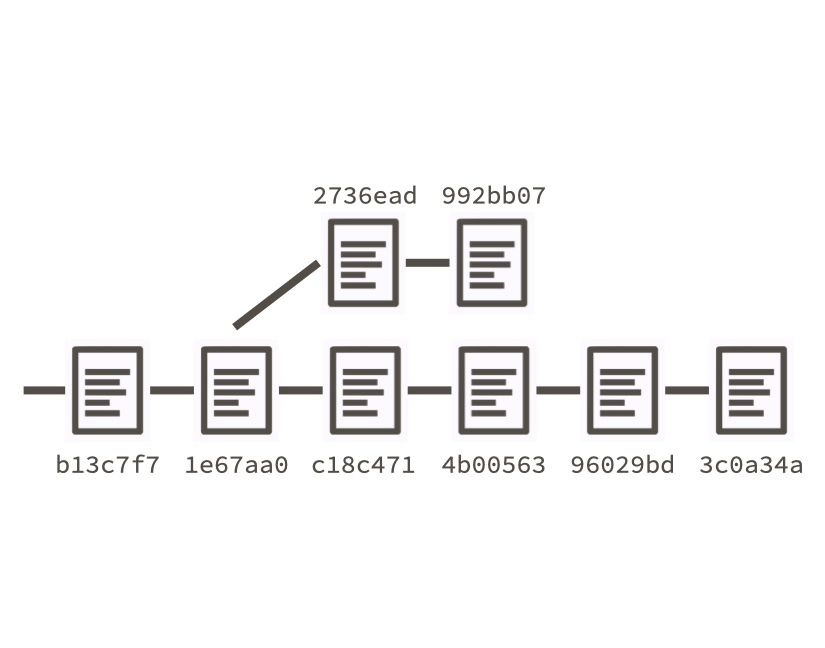
\includegraphics[width=0.6\linewidth]{img/refs-only-shas} \end{center}

Luckily, there are even more ways to talk about a specific commit, that are much easier for humans to wrap their head around.
These are called Git ``refs'', short for references and, if you're familiar with the programming concept of a pointer, that's exactly the right mental model.

\section{Useful refs}\label{useful-refs}

Here are some of the most useful refs:

\begin{itemize}
\tightlist
\item
  A branch name.
  Example: \texttt{main}, \texttt{wild-experiment}.
  When you refer to the \texttt{main} branch, that resolves to the SHA of the tip of
  the \texttt{main} branch.
  Think of a branch ref as a sliding ref that evolves as the branch does.
\end{itemize}

\begin{center}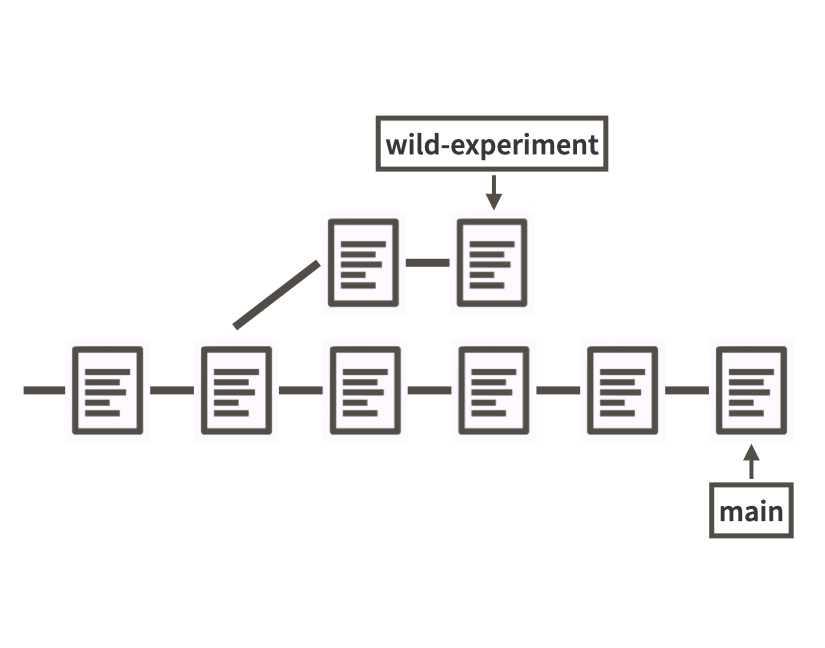
\includegraphics[width=0.6\linewidth]{img/refs-only-branches} \end{center}

\begin{itemize}
\tightlist
\item
  \texttt{HEAD}.
  This (almost always) resolves to the tip of the branch that is currently
  checked out.\footnote{When does \texttt{HEAD} not resolve to the SHA at the tip of some branch?
    When you are a \emph{detached HEAD} state.
    Detached HEAD!
    That sounds bad, but it's not intrinsically good or bad.
    It IS bad, though, to be in a detached HEAD state if you didn't mean to be and you don't understand the deal.
    You get into a detached HEAD state when you directly checkout a specific commit, as opposed to checking out or switching to a \emph{branch}.
    In experienced hands, this can be a legit thing to do.
    But in the meantime, I recommend that you always visit a specific state in the history by checking out a \emph{branch}, even if that means you need to create a temporary branch like \texttt{holder} or \texttt{time-travel}.
    To get out of the detached \texttt{HEAD} state, checkout some existing branch, with \texttt{git\ checkout\ main} or similar.
    Otherwise, the StackOverflow thread \href{https://stackoverflow.com/q/10228760}{How do I fix a Git detached head?} addresses many vexing detached \texttt{HEAD} scenarios.}
  You can think of \texttt{HEAD} as a ref that points to the tip of the current branch,
  which itself is a ref, that points to a specific SHA.
  There are two layers of indirection.
  This is also called a \emph{symbolic ref}.
\end{itemize}

\begin{center}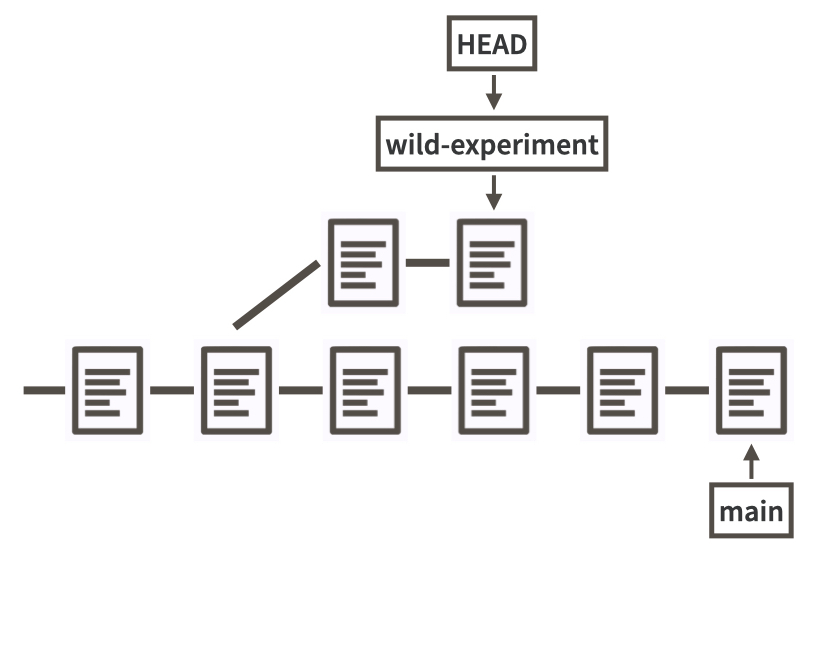
\includegraphics[width=0.6\linewidth]{img/refs-branches-and-HEAD-1} \end{center}

\begin{itemize}
\tightlist
\item
  A tag.
  Example: \texttt{v1.4.2}.
  Tags differ from branch refs and the \texttt{HEAD} ref in that they tend to be much
  more static.
  Tags aren't sliding by nature, although it is possible to reposition a tag to
  point at a new SHA, if you make an explicit effort.
  The most common use of a tag is to provide a nice label for a specific SHA.
\end{itemize}

\begin{center}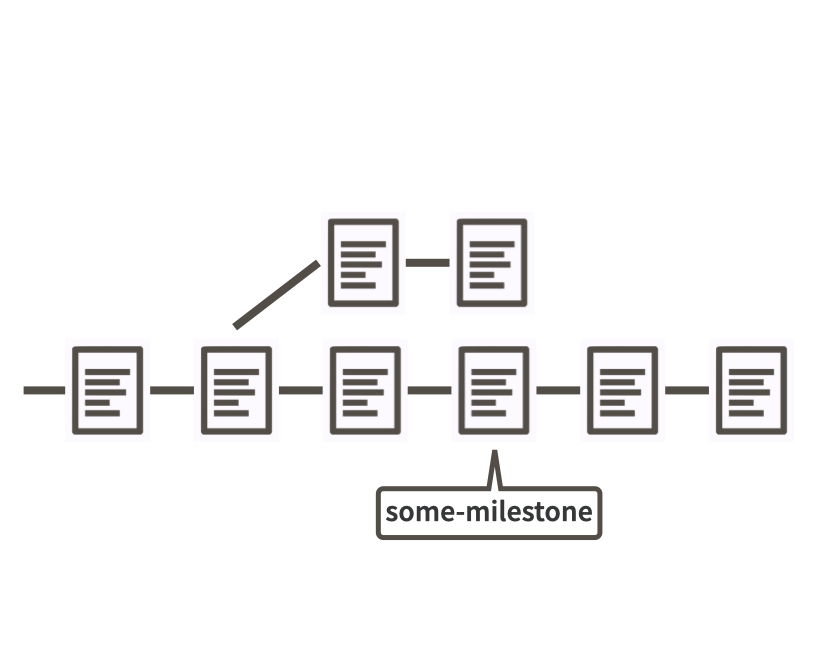
\includegraphics[width=0.6\linewidth]{img/refs-tag} \end{center}

If you'd like to make all of this more concrete, you can use \texttt{git\ rev-parse} in the shell to witness how refs resolve to concrete SHAs.
Here's the general pattern:

\begin{Shaded}
\begin{Highlighting}[]
\NormalTok{git rev{-}parse YOUR\_REF\_GOES\_HERE}
\end{Highlighting}
\end{Shaded}

Here are some examples executed in the Happy Git repo:

\begin{Shaded}
\begin{Highlighting}[]
\NormalTok{\textasciitilde{}/rrr/happy{-}git{-}with{-}r \% git rev{-}parse HEAD}
\NormalTok{631fee855db49d87f6c2a2cab474e89c11322bf4}

\NormalTok{\textasciitilde{}/rrr/happy{-}git{-}with{-}r \% git rev{-}parse main}
\NormalTok{631fee855db49d87f6c2a2cab474e89c11322bf4}

\NormalTok{\textasciitilde{}/rrr/happy{-}git{-}with{-}r \% git rev{-}parse testing{-}something                       }
\NormalTok{1eeb91d177b7cb5f9a0b29ebee3e6c0c8ff98f88}
\end{Highlighting}
\end{Shaded}

Notice that \texttt{HEAD} and \texttt{main} resolve to the same SHA, since the \texttt{main} branch was checked out at the time.
\texttt{testing-something} is the name of a branch that happened to be lying around.

These refs can be used in all sorts of Git operations, such as \texttt{git\ diff}, \texttt{git\ reset}, and \texttt{git\ checkout}:

\begin{Shaded}
\begin{Highlighting}[]
\NormalTok{git diff main testing{-}something}

\NormalTok{git reset testing{-}something {-}{-} README.md}

\NormalTok{git checkout {-}b my{-}new{-}branch main}
\end{Highlighting}
\end{Shaded}

\section{Relative refs}\label{relative-refs}

There are also modifiers that help you specify a commit relative to a ref, e.g.~``the commit just before this one''.

\texttt{HEAD\textasciitilde{}1} refers to the commit just before \texttt{HEAD}.
\texttt{HEAD\^{}} is another way to say exactly the same thing.

\begin{center}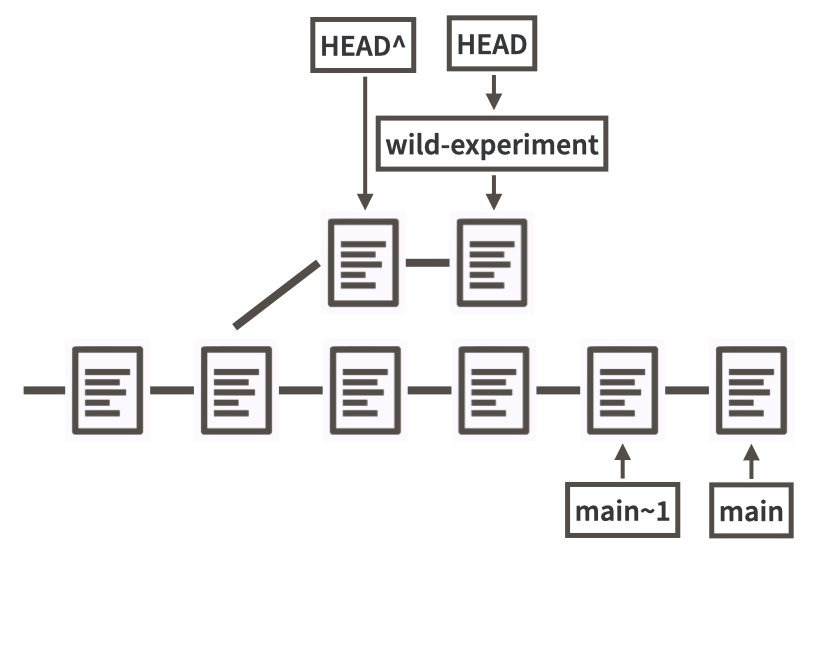
\includegraphics[width=0.6\linewidth]{img/refs-relative} \end{center}

Here are some examples executed in the Happy Git repo:

\begin{Shaded}
\begin{Highlighting}[]
\NormalTok{\textasciitilde{}/rrr/happy{-}git{-}with{-}r \% git rev{-}parse HEAD\textasciitilde{}1}
\NormalTok{5dacec4950a3746310bb30704417a792302b044a}

\NormalTok{\textasciitilde{}/rrr/happy{-}git{-}with{-}r \% git rev{-}parse HEAD\^{}}
\NormalTok{5dacec4950a3746310bb30704417a792302b044a}
\end{Highlighting}
\end{Shaded}

Notice that \texttt{HEAD\textasciitilde{}1} and \texttt{HEAD\^{}} resolve to the same SHA.

Both of these patterns generalize.
\texttt{HEAD\textasciitilde{}3} and \texttt{HEAD\^{}\^{}\^{}} are valid and equivalent refs.

I must admit that I am not a big fan of these relative ref shortcuts and especially not when reaching back more than one commit.
I worry that I have some sort of off-by-one error in my understanding and I'll end up targetting the wrong commit.

Tools like GitKraken and GitHub make it extremely easy to copy specific SHAs to your clipboard.
So when I need a ref that's not a simple branch name or tag, I almost always lean on user-friendly tools like GitKraken or GitHub to allow me to state my intent using the actual SHA of interest.
I suspect that the relative ref shortcuts are most popular with folks who are exclusively using command line Git and are operating under different constraints.
There's actually a rich set of ways to specify a target commit that goes well beyond the \texttt{\^{}} and \texttt{\textasciitilde{}} syntax shown here.
You can learn more in the \href{https://git-scm.com/docs/gitrevisions}{official Git documention about revision parameters}.

In GitKraken, right or control click on the target commit to access a menu that includes ``Copy commit sha'', among many other useful commands.
If you're using another Git client, there is probably a way to do this and it's worth figuring that out.

\begin{center}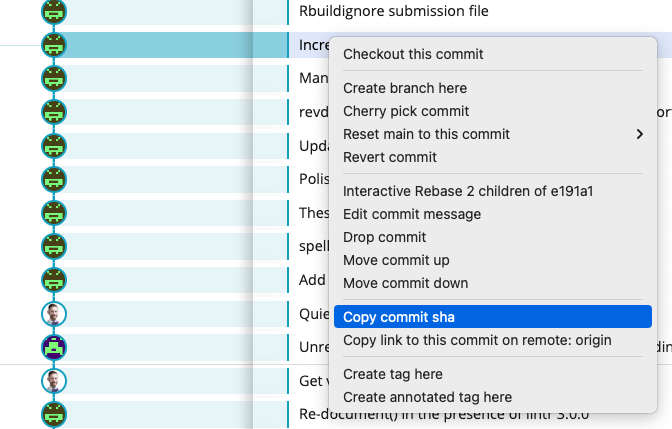
\includegraphics[width=0.6\linewidth]{img/gitkraken-screenshot-copy-commit-sha} \end{center}

GitHub also makes it extremely easy to copy a SHA in many contexts.
This screenshot shows just one example.
Once you start looking for this feature, you'll find it in many places on GitHub.

\begin{center}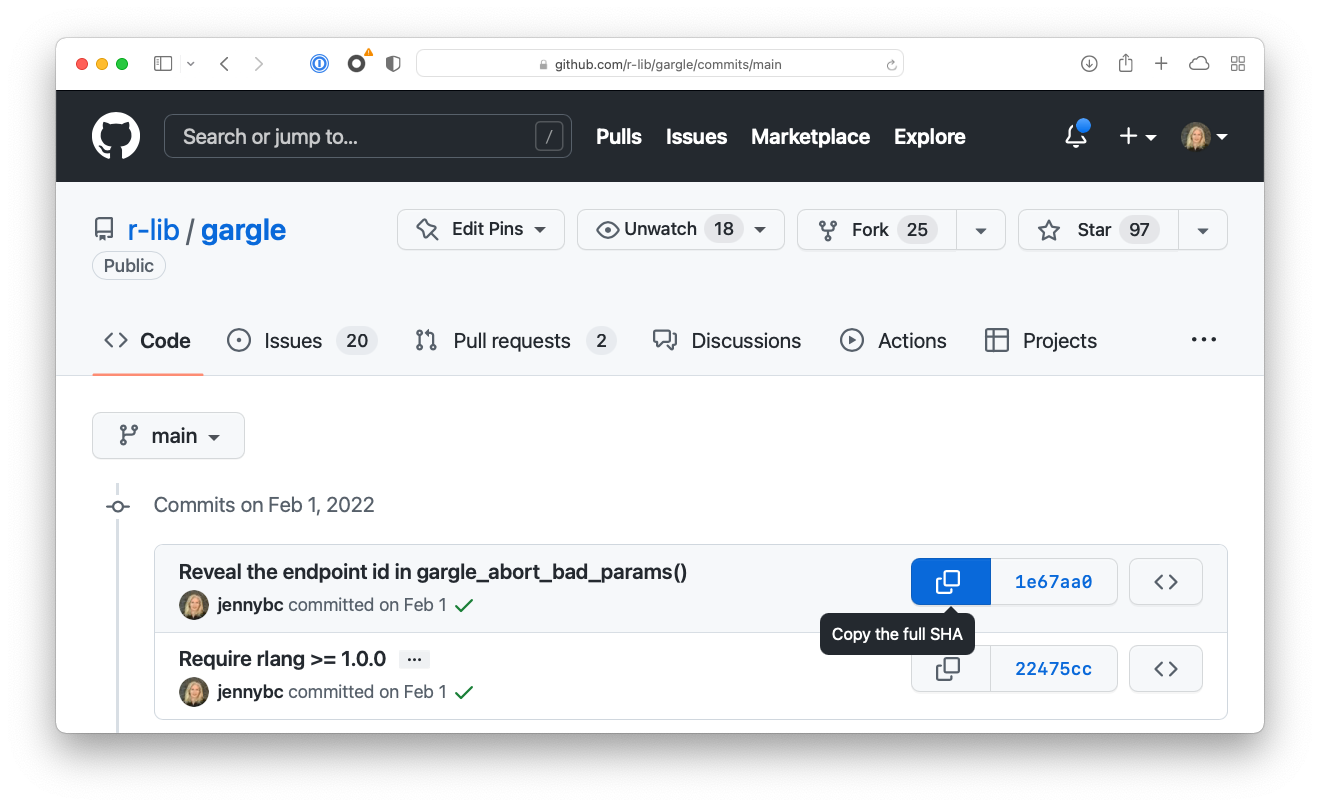
\includegraphics[width=0.6\linewidth]{img/github-screenshot-copy-the-full-sha} \end{center}

\part{Remote setups}\label{part-remote-setups}

\chapter*{Git remote setups}\label{remote-scenarios-intro}
\addcontentsline{toc}{chapter}{Git remote setups}

The previous part ended with some basics about \hyperref[git-remotes]{Git remotes}, such as how to define or rename one. Recall that a Git remote is another copy of the repo, usually living elsewhere (hence the term ``remote''), that you can pull changes from or push changes to. Remotes are the foundation for all collaborative Git work.

But knowing the mechanics of how to add or rename a remote does little good if you don't know \emph{why} or \emph{when} to do it. Luckily, we have very strong opinions about how you should set up your remotes, all motivated by getting you prepared for smooth, happy collaborative work.

In this part we describe various remote setups that are common (for better or worse) and what they are good for (or what's wrong with them and how to fix).

\chapter{Common remote setups}\label{common-remote-setups}

We only consider a very constrained set of remotes here:

\begin{itemize}
\tightlist
\item
  The remote is on GitHub, e.g.~its URL looks something like \texttt{https://github.com/OWNER/REPO.git} or \texttt{git@github.com:OWNER/REPO.git}.
\item
  The remote is named \texttt{origin} or \texttt{upstream}. These may not be the most evocative names in the world, but they are the most common choices.
\end{itemize}

If you use a different host or different remote names, you should still be able to translate these examples to your setting.

Along the way, we note how these setups relate to the usethis package, i.e.~how usethis can help you get into a favorable setup or how a favorable setup unlocks the full power of usethis.
Many of these operations -- including characterizing your GitHub remotes -- require that you have configured a GitHub personal access token.
See section \ref{get-a-pat} for more details on why and how to do that.
If you don't use usethis, feel free to ignore these asides.

\section{No GitHub}\label{no-github}

As a starting point, consider a local Git repo that is not yet connected to GitHub.

\begin{center}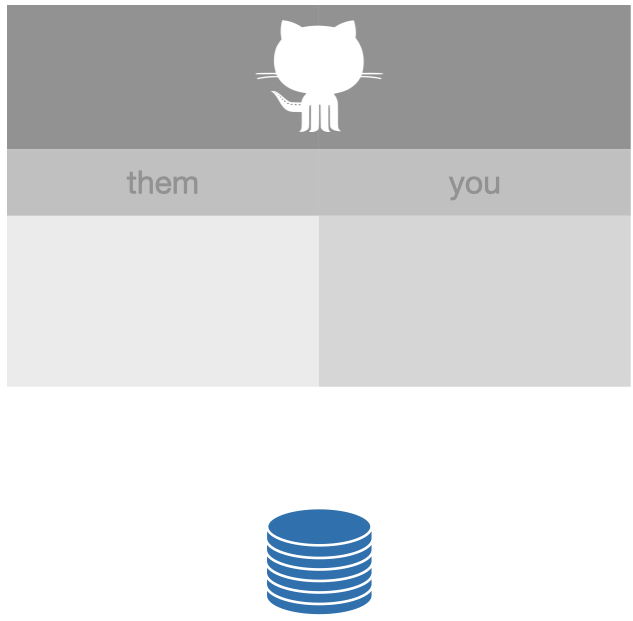
\includegraphics[width=0.6\linewidth]{img/no-github} \end{center}

This is not very exciting, but sets the stage for what's to come.
We introduce the icon we use for a Git repo, which looks like a stack of coins or a barrel.
This one is blue, which indicates you have write permission.

How to achieve:

\begin{itemize}
\tightlist
\item
  Command line Git: \texttt{git\ init}
\item
  With usethis, existing project: \texttt{usethis::use\_git()}
\item
  With RStudio:

  \begin{itemize}
  \tightlist
  \item
    Existing Project: \emph{Tools \textgreater{} Version Control \textgreater{} Project Setup}, select Git
    as the version control system
  \item
    New Project: Make sure ``Create a Git repository'' is selected
  \end{itemize}
\end{itemize}

usethis describes this setup as ``no\_github''.

\section{Ours (more specifically, yours)}\label{ours-you}

A common next step is to associate a local repo with a copy on GitHub, owned by you.

\begin{center}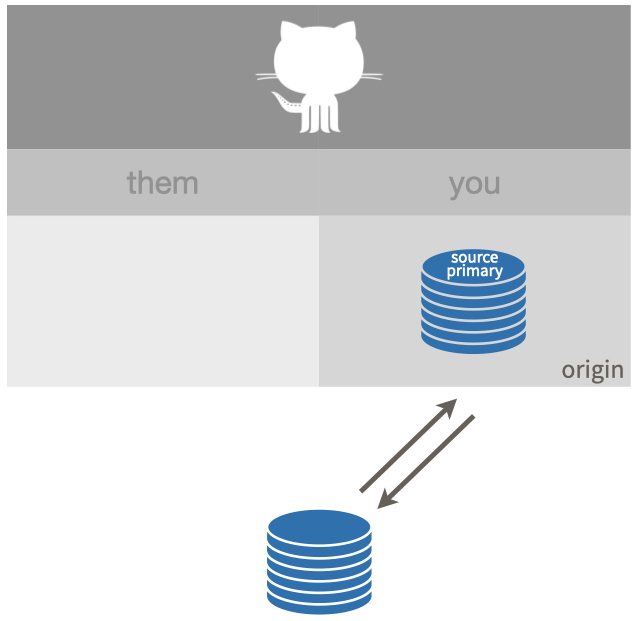
\includegraphics[width=0.6\linewidth]{img/ours-you} \end{center}

A remote named \texttt{origin} is configured and you have permission to push to (and pull from) \texttt{origin}.
(That's why \texttt{origin} is colored blue and there are solid arrows going both directions.)
The \texttt{origin} remote on GitHub is what we'll call a \textbf{source} repo, meaning it is not a fork (i.e.~copy) of anything else on GitHub.
In this case, \texttt{origin} is also what we'll call your \textbf{primary} repo, meaning it is the primary remote you interact with on GitHub (for this project).

How to achieve if the local repo exists first:

\begin{itemize}
\tightlist
\item
  Detailed instructions are in
  \hyperref[existing-github-last]{Existing project, GitHub last}.
\item
  With usethis: \texttt{usethis::use\_github()}.
\item
  Command line Git or RStudio: You can't complete this task fully from the
  command line or from RStudio:

  \begin{itemize}
  \tightlist
  \item
    Create a new GitHub repo in the browser, with the correct name,
    and capture its HTTPS or SSH URL.
  \item
    Configure the repo as the \texttt{origin} remote.
  \item
    Push.
  \item
    Even now, the setup may not be ideal, because upstream tracking
    relationships are probably not setup, which means you may not be able to
    push and pull easily. You may need to explicitly configure an upstream
    tracking branch for one or more local branches. Next time you want to
    create a GitHub repo from a local repo, consider using
    \texttt{usethis::use\_github()}, which completes all of this setup in one go.
  \end{itemize}
\end{itemize}

How to achieve if the remote repo exists first:

\begin{itemize}
\tightlist
\item
  Detailed instructions are in
  \hyperref[git-clone-usethis-rstudio]{New RStudio Project via git clone}.
\item
  With usethis: \texttt{usethis::create\_from\_github("OWNER/REPO",\ fork\ =\ FALSE)}
\item
  Command line: \texttt{git\ clone\ \textless{}URL\textgreater{}}, with the source repo's HTTPS or SSH URL
\item
  In RStudio: Capture the source repo's HTTPS or SSH URL and do
  \emph{File \textgreater{} New Project \textgreater{} Version Control \textgreater{} Git}.
\end{itemize}

usethis describes this setup as ``ours''.

\section{Ours}\label{ours-them}

Here is a variation on ``ours'' that is equivalent in practice.

\begin{center}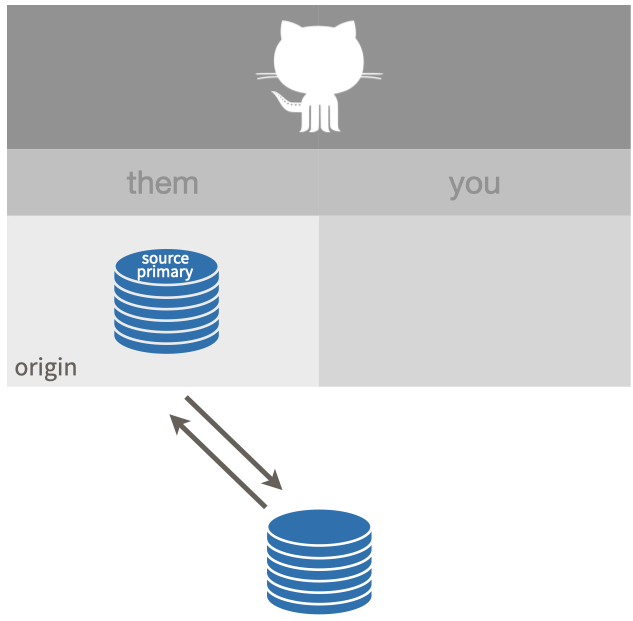
\includegraphics[width=0.6\linewidth]{img/ours-them} \end{center}

A remote named \texttt{origin} is configured and you can push to (and pull from) \texttt{origin}.
As above, \texttt{origin} is a \textbf{source} repo, meaning it is not a fork (or copy) of anything else on GitHub.
The \texttt{origin} remote is, however, not owned by you.
Instead it's owned by another GitHub user or organisation.
\texttt{origin} is also your \textbf{primary} repo in this setup.

How does this happen?

\begin{enumerate}
\def\labelenumi{\arabic{enumi}.}
\tightlist
\item
  The source repo is owned by an organisation and your role in this organisation confers enough power to create repos or to push to this repo.
\item
  The owner of the source repo has added you, specifically, as a collaborator to this specific repo.
\end{enumerate}

How to achieve? The procedure is the same as for the previous ``ours'' setup. But remember to specify \texttt{usethis::use\_github(organisation\ =\ "ORGNAME")} if you want to create a new repo under an organisation, instead of your personal account.

usethis describes this setup as ``ours''.

\section{Theirs}\label{theirs}

This is a setup that many people get themselves into, when it's not actually what they need.
It's not broken \emph{per se}, but it's limiting.

\begin{center}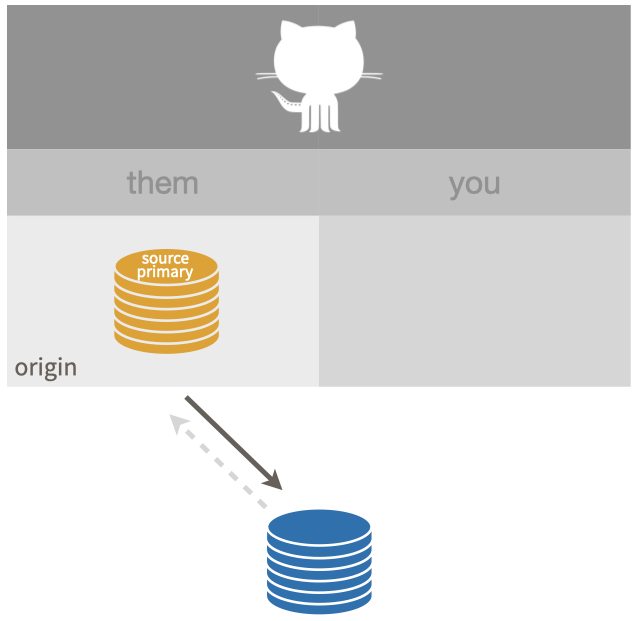
\includegraphics[width=0.6\linewidth]{img/theirs} \end{center}

You cannot push to \texttt{origin}, which is both the source repo and your primary repo.
(This is indicated by the orange color of \texttt{origin} and the greyed out, dashed ``push'' arrow.)
\texttt{origin} is read-only for you.

If you are taking a repo for a quick test drive, this configuration is fine.
But there is no way to get changes back into the source repo, since you cannot push to it and you haven't created a fork, which is necessary for a pull request.

How does this happen?

\begin{itemize}
\tightlist
\item
  Cloning the source repo, either via \texttt{git\ clone\ \textless{}URL\textgreater{}} (command line) or through a Git client, e.g.~RStudio's \emph{File \textgreater{} New Project \textgreater{} Version Control \textgreater{} Git} workflow.
\item
  Calling \texttt{usethis::create\_from\_github("OWNER/REPO",\ fork\ =\ FALSE)}.
\end{itemize}

usethis describes this setup as ``theirs''.

What if you do want to make a pull request?
This means you should have done \emph{fork-and-clone} instead of \emph{clone}.
If you've made no changes or they're easy to save somewhere temporarily, just start over with a fork-and-clone workflow (fully explained in \ref{fork-and-clone}) and re-introduce your changes.
It is also possible to preserve your work in a local branch, fork the source repo, re-configure your remotes, re-sync up with the source repo, and get back on track.
But this is much easier to goof up.
And remember to fork and clone (not just clone) in the future!

\section{Fork (of theirs)}\label{fork-them}

This is an ideal setup if you want to make a pull request and generally follow the development of a source repo owned by someone else.

\begin{center}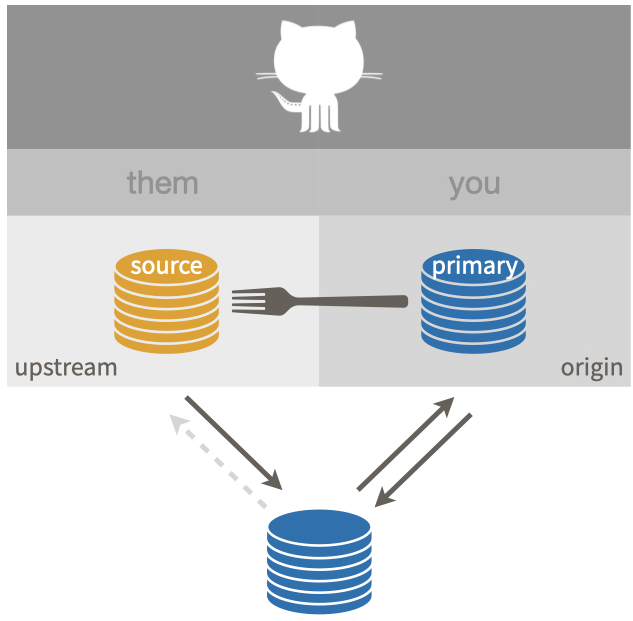
\includegraphics[width=0.6\linewidth]{img/fork-them} \end{center}

This shows a successful ``fork-and-clone''.
Your local repo can pull changes from the source repo, which is configured as \texttt{upstream}, which you cannot push to (but you can pull from).
You have a fork of the source repo (a very special copy, on GitHub) and it is configured as \texttt{origin}.
\texttt{origin} is your primary repo.
You can push to and pull from \texttt{origin}.
You can make a pull request back to the source repo via your fork.

usethis describes this setup as ``fork''.

How to achieve:

\begin{itemize}
\tightlist
\item
  Detailed instructions are given in \hyperref[fork-and-clone]{Fork and clone}.
\item
  With usethis: \texttt{usethis::create\_from\_github("OWNER/REPO",\ fork\ =\ TRUE)}
\item
  Command line Git or RStudio: You can't complete this task fully from the
  command line or RStudio:

  \begin{itemize}
  \tightlist
  \item
    Fork the source repo in the browser, capture the HTTPS or SSH
    URL of \textbf{your fork}, then use \texttt{git\ clone\ \textless{}FORK\_URL\textgreater{}}
    (command line) or RStudio's \emph{File \textgreater{} New Project \textgreater{} Version Control \textgreater{} Git}
    workflow. But, wait, you're not done! If you stop here, you will have the
    incomplete setup we refer to as
    \hyperref[fork_upstream_is_not_origin_parent]{``fork (salvageable)''}, below.
  \item
    You still need to add the source repo as the \texttt{upstream} remote. Capture
    the HTTPS or SSH URL of the \textbf{source repo}. At the command line, do \texttt{git\ \ \ remote\ add\ upstream\ \textless{}SOURCE\_URL\textgreater{}} or click RStudio's \emph{New Branch} button,
    which brings up a window where you can add the \texttt{upstream} remote.
  \item
    Even then, the setup may not be ideal, because your local default branch
    is probably tracking \texttt{origin}, not \texttt{upstream}, which is preferable for
    a fork. \texttt{usethis::create\_from\_github()} completes all of this setup in
    one go.
  \item
    These last two steps are described in
    \hyperref[fork-and-clone-finish]{Finish the fork and clone setup}.
  \end{itemize}
\end{itemize}

\section{Fork (of ours)}\label{fork-of-ours}

This is a less common variation on the fork setup.

\begin{center}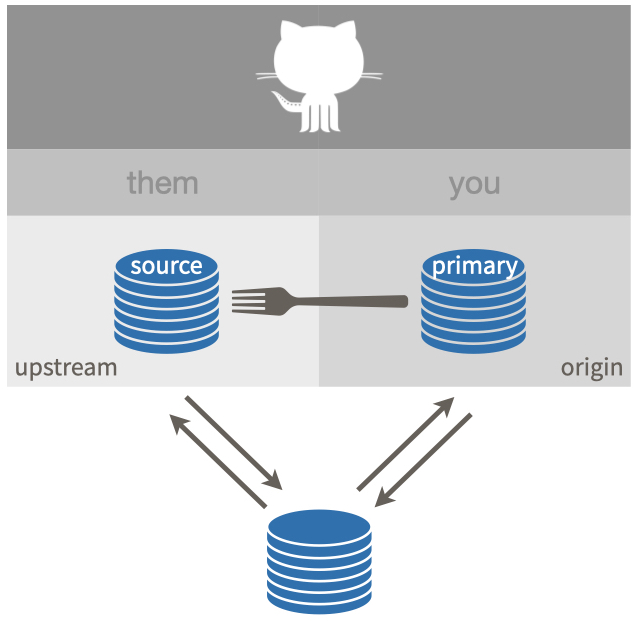
\includegraphics[width=0.6\linewidth]{img/fork-ours} \end{center}

In this case, you have permission to push to the source repo, but you elect to create a personal fork anyway.
Certain projects favor this approach and it offers maximum development flexibility for advanced users.
However, most users are better served by the simpler ``ours'' setup in this case.

How to achieve:

\begin{itemize}
\tightlist
\item
  In general, it's the same as the regular \hyperref[fork-them]{fork setup} above.
\item
  With usethis, make sure to explicitly specify \texttt{fork\ =\ TRUE}, i.e.~do
  \texttt{usethis::create\_from\_github("OWNER/REPO",\ fork\ =\ TRUE)}.
\end{itemize}

usethis describes this setup as ``fork''.

\section{Fork (salvageable)}\label{fork_upstream_is_not_origin_parent}

Here is one last fork setup that's sub-optimal, but it can be salvaged.

\begin{center}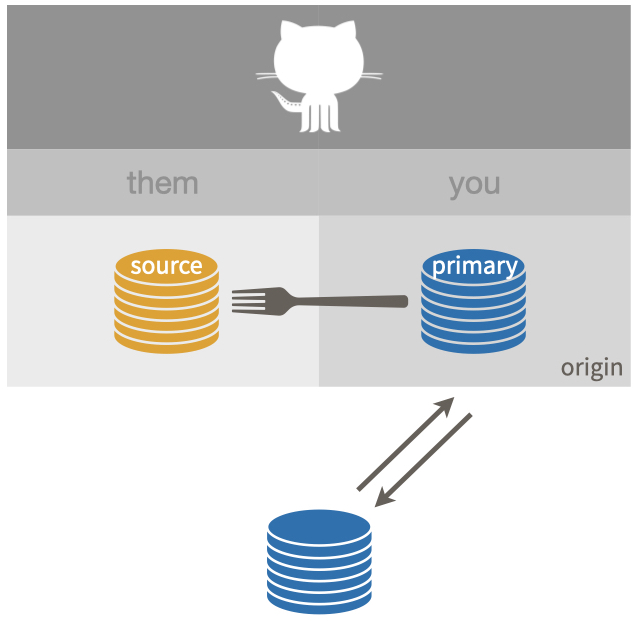
\includegraphics[width=0.6\linewidth]{img/fork_upstream_is_not_origin_parent} \end{center}

This is what happens when you do fork-and-clone and you \emph{only} do fork-and-clone.
What's missing is a connection back to the source repo.

How does this happen?

\begin{itemize}
\tightlist
\item
  Cloning your own fork, either via \texttt{git\ clone} in the shell or through a Git client, such as RStudio. And then stopping here.
\end{itemize}

If you only plan to make one pull request, this setup is fine.
When the exchange is done, delete your local repo and your fork and move on with your life.
You can always re-fork in the future.
But if your pull request stays open for a while or if you plan to make repeated contributions, you'll need to pull ongoing developments in the source repo into your local copy.

You can convert this into the ideal \hyperref[fork-them]{fork setup} like so:

\begin{itemize}
\tightlist
\item
  Detailed instructions are in
  \hyperref[fork-and-clone-finish]{Finish the fork and clone setup}.
\item
  Add the source repo as the \texttt{upstream} remote.
\item
  Set \texttt{upstream/main} as the upstream tracking branch for local \texttt{main}
  (substitute whatever your default branch is called).
\end{itemize}

Next time you do fork-and-clone, consider using \texttt{usethis::create\_from\_github(fork\ =\ TRUE)} instead, which completes all of this setup in one go.

usethis describes this setup as ``fork\_upstream\_is\_not\_origin\_parent''.

\chapter{Equivocal remote setups}\label{equivocal}

Just like the previous section about the most common setups, we only consider a very constrained set of remotes:

\begin{itemize}
\tightlist
\item
  The remote is on GitHub, e.g.~its URL looks something like \texttt{https://github.com/OWNER/REPO.git} or \texttt{git@github.com:OWNER/REPO.git}.
\item
  The remote is named \texttt{origin} or \texttt{upstream}.
\end{itemize}

The setups described here are characterized by \emph{incomplete information}.
This section exists mostly to explain feedback that the usethis package might give about a GitHub remote configuration.

To identify any of the remote setups described in section \ref{common-remote-setups}, we need information from GitHub:

\begin{itemize}
\tightlist
\item
  Whether you can push to a repo
\item
  Whether a repo is a fork
\item
  For a fork, what is its source repo
\end{itemize}

Sometimes some of this information is publicly available, but some of it never is, such as repo permissions.
This means that programmatic access to this information, i.e.~requests to the GitHub API, generally requires authorization by an authenticated GitHub user.

This means that client packages, like usethis, work best when you have configured a GitHub personal access token (PAT).
See section \ref{get-a-pat} for more details on why and how to do that.

If you've configured a PAT and are being told your GitHub config is problematic, consider these other explanations:
Are you offline?
Is GitHub down?
Have you lost permission to access the repo?
Has your PAT expired?
By default, they now expire after 30 days.

\section{Maybe ``ours'' or ``theirs''}\label{maybe-ours-or-theirs}

When we detect just one GitHub remote, but we can't verify the info above, usethis describes the setup as ``maybe\_ours\_or\_theirs''.

\begin{center}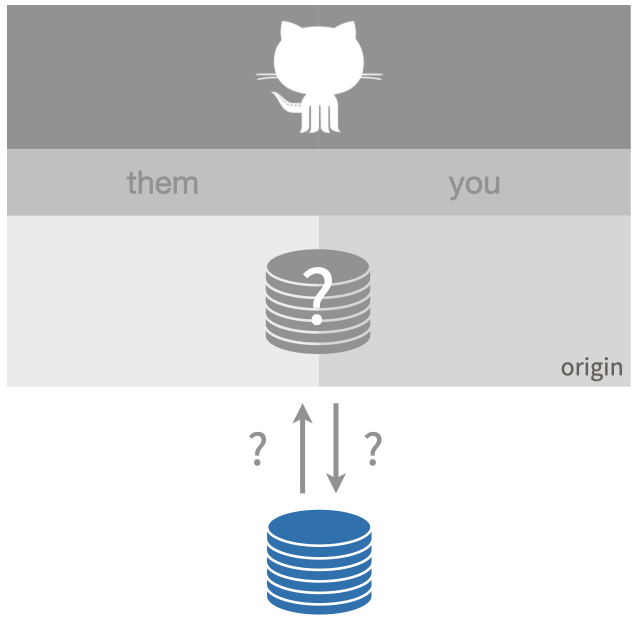
\includegraphics[width=0.6\linewidth]{img/maybe_ours_or_theirs} \end{center}

Once a PAT is available, this setup can be identified as being \hyperref[ours-you]{``ours'' (belonging to you)}, \hyperref[ours-them]{``ours'' (but belonging to someone else)}, or \hyperref[theirs]{``theirs''}.

\section{Maybe fork}\label{maybe-fork}

When we detect two GitHub remotes, but we can't verify the info above, usethis describes the setup as ``maybe\_fork''.

\begin{center}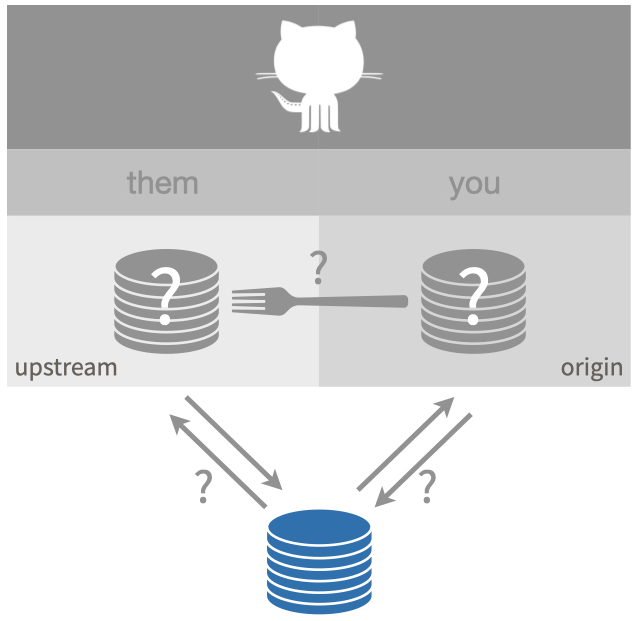
\includegraphics[width=0.6\linewidth]{img/maybe_fork} \end{center}

Once a PAT is available, this setup can be identified as being a well-configured \hyperref[fork-them]{fork} or a \hyperref[fork_upstream_is_not_origin_parent]{fork with incomplete setup} (or possibly something more weird).

\section{How to fix}\label{how-to-fix}

These setups aren't necessarily broken, but usethis needs more information to operate.

To ``fix'' this, set up a GitHub personal access token.
See section \ref{get-a-pat} for more details on why and how to do that.

\part{Daily Workflows}\label{part-daily-workflows}

\chapter*{Useful Git patterns for real life}\label{workflows-intro}
\addcontentsline{toc}{chapter}{Useful Git patterns for real life}

\emph{Much of this originates as live workshop materials; the unlinked workflows are planned but not yet converted to prose here.}

Git patterns that come up frequently in real work:

\begin{itemize}
\tightlist
\item
  Commit early and often. Push less often. \hyperref[repeated-amend]{The Repeated Amend}.
\item
  \hyperref[push-rejected]{Help, my push was rejected!}
\item
  \hyperref[pull-tricky]{Integrating remote and local work}. Probably so you can push again.
\item
  Burn it all down.
\item
  Time travel:

  \begin{itemize}
  \tightlist
  \item
    \hyperref[time-travel-see-past]{``I just need to see the past''.} Browse and search on GitHub.
  \item
    ``I need to visit the past''. Create a checkout a branch.
  \item
    ``I want to return to the past''. \texttt{git\ revert}, \texttt{git\ reset}
  \item
    ``I had a great cookie last October''. \texttt{git\ cherry\ pick}, \texttt{git\ checkout\ REF\ -\/-\ path}
  \end{itemize}
\end{itemize}

Play well with others:

\begin{itemize}
\tightlist
\item
  \hyperref[fork-and-clone]{Fork and clone}.
\item
  \hyperref[upstream-changes]{Get upstream changes for a fork}.
\item
  Disposable fork.
\item
  \hyperref[workflows-browsability]{Make your repo rewarding to browse on GitHub}.
\item
  \hyperref[pr-extend]{Explore and extend a pull request}
\end{itemize}

\chapter{The Repeated Amend}\label{repeated-amend}

One of the principal joys of version control is the freedom to experiment without fear.
If you make a mess of things, you can always go back to a happier version of your project.
We describe several methods of such time travel in \emph{link to come}.
But you must have a good commit to fall back to!

\section{Rock climbing analogy}\label{rock-climbing-analogy}

Using a Git commit is like using anchors and other protection when climbing. If you're crossing a dangerous rock face you want to make sure you've used protection to catch you if you fall. Commits play a similar role: if you make a mistake, you can't fall past the previous commit. Coding without commits is like free-climbing: you can travel much faster in the short-term, but in the long-term the chances of catastrophic failure are high! Like rock climbing protection, you want to be judicious in your use of commits. Committing too frequently will slow your progress; use more commits when you're in uncertain or dangerous territory. Commits are also helpful to others, because they show your journey, not just the destination.

R Packages, Hadley Wickham (Wickham (\citeproc{ref-r-pkgs-book}{2015}))

Let's talk about this:

\begin{quote}
use more commits when you're in uncertain or dangerous territory
\end{quote}

When I'm doing something tricky, I often proceed towards my goal in small increments, checking that everything still works along the way.
Yes it works?
Make a commit.
This is my new worst case scenario.
Keep going.

What's not to love?

This can lead to an awful lot of tiny commits.
This is absolutely fine and nothing to be ashamed of.
But one day you may start to care about the utility and aesthetics of your Git history.

The Repeated Amend is a pattern where, instead of cluttering your history with lots of tiny commits, you build up a ``good'' commit gradually, by amending.

\emph{Yes, there are other ways to do this, e.g.~via squashing and interactive rebase, but I think amending is the best way to get started.}

\section{Workflow sketch}\label{workflow-sketch}

\subsection{Initial condition}\label{initial-condition}

Start with your project in a functional state:

\begin{itemize}
\tightlist
\item
  R package? Run your tests or \texttt{R\ CMD\ check}.
\item
  Data analysis? Re-run your script or re-render your \texttt{.Rmd} with the new chunk.
\item
  Website or book? Make sure the project still compiles.
\item
  You get the idea.
\end{itemize}

Make sure your ``working tree is clean'' and you are synced up with your GitHub remote. \texttt{git\ status} should show something like:

\begin{Shaded}
\begin{Highlighting}[]
\NormalTok{\textasciitilde{}/tmp/myrepo \% git status                                                          }
\NormalTok{On branch main}
\NormalTok{Your branch is up to date with \textquotesingle{}origin/main\textquotesingle{}.}

\NormalTok{nothing to commit, working tree clean}
\end{Highlighting}
\end{Shaded}

\subsection{Get to work}\label{get-to-work}

Imagine we start at commit C, with previous commit B and, before that, A:

\begin{Shaded}
\begin{Highlighting}[]
\ExtensionTok{...} \AttributeTok{{-}{-}}\NormalTok{ A }\AttributeTok{{-}{-}}\NormalTok{ B }\AttributeTok{{-}{-}}\NormalTok{ C}
\end{Highlighting}
\end{Shaded}

Make a small step towards your goal.
Re-check that your project ``works''.

Stage those changes with and make a commit with the message ``WIP'', meaning ``work in progress''.
Do this in RStudio or in the shell (Appendix \ref{shell}):

\begin{Shaded}
\begin{Highlighting}[]
\NormalTok{git add path/to/the/changed/file}
\NormalTok{git commit {-}m "WIP"}
\end{Highlighting}
\end{Shaded}

The message can be anything, but ``WIP'' is a common convention.
If you use it, whenever you return to a project where the most recent commit message is ``WIP'', you'll know that you were probably in the middle of something.
If you push a ``WIP'' commit, on purpose or by mistake, it signals to other people that more commits might be coming.

Your history now looks like this:

\begin{Shaded}
\begin{Highlighting}[]
\ExtensionTok{A} \AttributeTok{{-}{-}}\NormalTok{ B }\AttributeTok{{-}{-}}\NormalTok{ C }\AttributeTok{{-}{-}}\NormalTok{ WIP}\PreprocessorTok{*}
\end{Highlighting}
\end{Shaded}

\textbf{Don't push!}
The \texttt{*} above signifies a commit that exists only in your local repo, not (yet) on GitHub.
If you called \texttt{git\ status}, you'd see something like ``Your branch is ahead of `origin/main' by 1 commit.'', which is also displayed in RStudio's Git pane.

Do a bit more work.
Re-check that your project is still in a functional state.
Stage and commit again, but this time \textbf{amend} your previous commit.
RStudio offers a check box for ``Amend previous commit'' or in the shell:

\begin{Shaded}
\begin{Highlighting}[]
\NormalTok{git commit {-}{-}amend {-}{-}no{-}edit}
\end{Highlighting}
\end{Shaded}

The \texttt{-\/-no-edit} part retains the current commit message of ``WIP''.

\textbf{Don't push!} Your history now looks like this:

\begin{Shaded}
\begin{Highlighting}[]
\ExtensionTok{A} \AttributeTok{{-}{-}}\NormalTok{ B }\AttributeTok{{-}{-}}\NormalTok{ C }\AttributeTok{{-}{-}}\NormalTok{ WIP}\PreprocessorTok{*}
\end{Highlighting}
\end{Shaded}

but the changes associated with the \texttt{WIP*} commit now represent your last two commits, i.e.~all the accumulated changes since state C.

Keep going like this.

Let's say you've finally achieved your goal. One last time, check that your project is functional and in a state you're willing to share with others.

Commit, amending again, but with a real commit message this time.
Think of this as commit D.
Push.
Do this in RStudio or the shell:

\begin{Shaded}
\begin{Highlighting}[]
\NormalTok{git commit {-}{-}amend {-}m "Implement awesome feature; closes \#43"}
\NormalTok{git push}
\end{Highlighting}
\end{Shaded}

Your history -- and that on GitHub -- look like this:

\begin{Shaded}
\begin{Highlighting}[]
\ExtensionTok{A} \AttributeTok{{-}{-}}\NormalTok{ B }\AttributeTok{{-}{-}}\NormalTok{ C }\AttributeTok{{-}{-}}\NormalTok{ D}
\end{Highlighting}
\end{Shaded}

As far as the world knows, you implemented the feature in one fell swoop.
But you got to work on the task incrementally, with the peace of mind that you could never truly break things.

\section{What if I need to fall back?}\label{what-if-i-need-to-fall-back}

Imagine you're in the middle of a Repeated Amend workflow:

\begin{Shaded}
\begin{Highlighting}[]
\NormalTok{A {-}{-} B {-}{-} C {-}{-} WIP*}
\end{Highlighting}
\end{Shaded}

and you make some changes that break your project, e.g.~tests start failing.
These bad changes are not yet committed, but they are saved.
You want to fall back to the last good state, represented by \texttt{WIP*}.

In Git lingo, you want to do a \textbf{hard reset} to the \texttt{WIP*} state.
Your local files will be forcibly reset to their state as of the \texttt{WIP*} commit.
With the command line:

\begin{Shaded}
\begin{Highlighting}[]
\NormalTok{git reset {-}{-}hard}
\end{Highlighting}
\end{Shaded}

which is implicitly the same as

\begin{Shaded}
\begin{Highlighting}[]
\NormalTok{git reset {-}{-}hard HEAD}
\end{Highlighting}
\end{Shaded}

which says: ``reset my files to their state at the most recent commit''.

This is also possible in RStudio.
In fact, the RStudio way makes it easier to selectively reset only specific files or only certain changes.
Click on ``Diff'' or ``Commit''.
Select a file with changes you do not want.
Use ``Discard All'' to discard all changes in that file.
Use ``Discard chunk'' to discard specific changes in a file.
Repeat this procedure for each affected file until you are back to an acceptable state.
Carry on.

If you committed a bad state, go to \emph{link to come} for more reset scenarios.

\section{Why don't we push intermediate progress?}\label{why-dont-we-push-intermediate-progress}

Amending a commit is an example of what's called ``rewriting Git history''.

Rewriting history that has already been pushed to GitHub -- and therefore potentially pulled by someone else -- is a controversial practice.
Like most controversial practices, lots of people still indulge in it, as do I.

But there is the very real possibility that you create headaches for yourself and others, so in Happy Git we must recommend that you abstain.
Once you've pushed something, consider it written in stone and move on.

\section{Um, what if I did push?}\label{um-what-if-i-did-push}

I told you not to!

But OK here we are.

Let's imagine you pushed this state to GitHub by mistake:

\begin{Shaded}
\begin{Highlighting}[]
\NormalTok{A {-}{-} B {-}{-} C {-}{-} WIP (85bf30a)}
\end{Highlighting}
\end{Shaded}

and proceeded to \texttt{git\ commit\ -\/-amend} again locally, leading to this state:

\begin{Shaded}
\begin{Highlighting}[]
\NormalTok{A {-}{-} B {-}{-} C {-}{-} WIP* (6e884e6)}
\end{Highlighting}
\end{Shaded}

I'm deliberately showing two histories that sort of look the same, in terms of commit messages.
But the last SHA reveals they are actually different.

You are in a pickle now, as you can't do a simple push or pull.
A push will be rejected and a pull will probably lead to a merge that you don't want.

You have two choices:

\begin{itemize}
\item
  If you have collaborators who may have pulled the repo at commit
  \texttt{WIP\ (85bf30a)}, you have to regard that particular history as being written
  in stone now.
  If there is any very precious work that only exists locally, such as a
  specific file, save a copy of that to a new file path, temporarily.
  Hard reset your local repo to \texttt{C} (\texttt{git\ reset\ -\/-hard\ HEAD\^{}}) and pull from
  GitHub.
  GitHub and local history now show this:

\begin{Shaded}
\begin{Highlighting}[]
\NormalTok{A {-}{-} B {-}{-} C {-}{-} WIP (85bf30a)}
\end{Highlighting}
\end{Shaded}

  If you saved some precious work to a temporary file path, bring it back into
  the repo now; save, stage, commit, and push.
  GitHub and local history now show this:

\begin{Shaded}
\begin{Highlighting}[]
\NormalTok{A {-}{-} B {-}{-} C {-}{-} WIP (85bf30a) {-}{-} E}
\end{Highlighting}
\end{Shaded}
\item
  If you have no collaborators or you have reason to believe they have not
  pulled, you can rewrite history, even on GitHub.
  You might as well make sure your local commit has a real, non-``WIP'' message
  at this point.
  Force push your history to GitHub (\texttt{git\ push\ -\/-force}).
  GitHub and local history now show this:

\begin{Shaded}
\begin{Highlighting}[]
\NormalTok{A {-}{-} B {-}{-} C {-}{-} D}
\end{Highlighting}
\end{Shaded}
\end{itemize}

In both cases, you've made the changes you want and your local repo and the
GitHub remote are synced up again.
The history is nicer in the second case, but that's a secondary issue.

\emph{There are many different ways to rewrite history and rescue some of these situations, but we find the approaches described above to be very approachable.}

\chapter{Dealing with push rejection}\label{push-rejected}

Problem: You want to push changes to GitHub, but you are rejected like so:

\begin{Shaded}
\begin{Highlighting}[]
\ExtensionTok{$}\NormalTok{ git push}
\ExtensionTok{To}\NormalTok{ https://github.com/YOU/REPO.git}
 \OtherTok{! }\ExtensionTok{[rejected]}\NormalTok{        main }\AttributeTok{{-}}\OperatorTok{\textgreater{}}\NormalTok{ main }\ErrorTok{(}\ExtensionTok{fetch}\NormalTok{ first}\KeywordTok{)}
\ExtensionTok{error:}\NormalTok{ failed to push some refs to }\StringTok{\textquotesingle{}https://github.com/YOU/REPO.git\textquotesingle{}}
\ExtensionTok{hint:}\NormalTok{ Updates were rejected because the remote contains work that you do}
\ExtensionTok{hint:}\NormalTok{ not have locally. This is usually caused by another repository pushing}
\ExtensionTok{hint:}\NormalTok{ to the same ref. You may want to first integrate the remote changes}
\ExtensionTok{hint:} \ErrorTok{(}\ExtensionTok{e.g.,} \StringTok{\textquotesingle{}git pull ...\textquotesingle{}}\KeywordTok{)} \ExtensionTok{before}\NormalTok{ pushing again.}
\ExtensionTok{hint:}\NormalTok{ See the }\StringTok{\textquotesingle{}Note about fast{-}forwards\textquotesingle{}}\NormalTok{ in }\StringTok{\textquotesingle{}git push {-}{-}help\textquotesingle{}}\NormalTok{ for details.}
\end{Highlighting}
\end{Shaded}

This means that your local Git history and that on the GitHub remote are not compatible, i.e.~they have diverged.

I suggest that you use \texttt{git\ status}, your \hyperref[git-client]{Git client}, or visit your GitHub remote in the browser to get more information about the situation, i.e.~to get a sense of this work that you do not have.

In the abstract, this is the state on GitHub:

\begin{verbatim}
A -- B -- C (on GitHub)
\end{verbatim}

And this is your local state:

\begin{verbatim}
A -- B -- D (what you have)
\end{verbatim}

You can't cause some sort of merge to happen to the GitHub copy when you push.

Instead, you've got to pull the commit \texttt{C} and somehow integrate it into your \texttt{D}-containing history. Then you will be able to push again.

This is covered in the workflow \hyperref[pull-tricky]{Pull, but you have local work}.

But before you behold the full horror of that, this is a great time to reflect on what we can learn from this situation.

\section{She who pushes first wins!}\label{she-who-pushes-first-wins}

You may have noticed that you -- the author of \texttt{D} -- are faffing around with Git more than the person who committed and pushed \texttt{C}, i.e.~your collaborator.

There is a lesson to be learned here!

If you had pushed \texttt{D} first, you'd be relaxing and they'd be figuring out how to integrate \texttt{C} into their history in order to push. So push your work often. Don't go dark and work ``offline'' for long stretches of time.

Obviously, you should push work to \texttt{main} because it's ``ready'' to share (or at least ``ready enough''), not to avoid Git merges.

There is a truly legitimate point here: It is better for the overall health of a project to be committing, pushing, and integrating more often, not less. This does not eliminate the need to integrate different lines of work, but it makes each integration smaller, less burdensome, and less prone to error.

\section{Stay in touch}\label{stay-in-touch}

Another take away is this: the sooner you know about \texttt{C}, the better. Pull (or fetch) often.

Let's think about your commit \texttt{D}. Maybe it was built up over a couple of days via the \hyperref[repeated-amend]{Repeated Amend pattern}. Maybe \texttt{C} was sitting there on GitHub the whole time or appeared very early in your process.

Consider that it might be easier to integrate \texttt{C} into your work \texttt{D} sooner rather than later. Sometimes this is not true, but more often it is.

In general, it pays off to be proactively aware of what others are doing (e.g.~to pull or fetch often) than to always be in reactive mode, learning about your collaborator's work only when your push is rejected.

\section{Use branches}\label{use-branches}

Finally, your early experiences collaborating with others and yourself in \texttt{main} will give you a visceral understanding of why most Git users eventually start to use \hyperref[git-branches]{branches}.

Branches afford explicit workflows for integrating different lines of work on your own terms. This is much nicer than trying to do a tricky merge or rebase in a frustrated panic, because you need to push your work to GitHub at the end of the day.

\chapter{Pull, but you have local work}\label{pull-tricky}

Problem: You want to pull changes from upstream, but you have done some new work locally since the last time you pulled. This often comes up because \hyperref[push-rejected]{what you actually want to do is \emph{push}}, but Git won't let you until you first incorporate the upstream changes.

For the sake of simplicity, assume we're dealing with the \texttt{main} branch and the remote is called \texttt{origin}.

Recent commit history of \texttt{origin/main}:

\begin{Shaded}
\begin{Highlighting}[]
\ExtensionTok{A{-}{-}B{-}{-}C}
\end{Highlighting}
\end{Shaded}

Recent commit history of the local \texttt{main} branch:

\begin{Shaded}
\begin{Highlighting}[]
\ExtensionTok{A{-}{-}B{-}{-}D}
\end{Highlighting}
\end{Shaded}

or maybe

\begin{Shaded}
\begin{Highlighting}[]
\ExtensionTok{A{-}{-}B{-}{-}}\ErrorTok{(}\ExtensionTok{uncommitted}\NormalTok{ changes}\KeywordTok{)}
\end{Highlighting}
\end{Shaded}

Your goal: get commit \texttt{C} into your local branch, while retaining the work in commit \texttt{D} or your uncommitted changes.

\begin{itemize}
\tightlist
\item
  Local state is \texttt{A-\/-B-\/-(uncommitted\ changes)}: You could use \texttt{git\ stash}. Or you could just make a commit to simplify your life (see next bullet).
\item
  Local state is \texttt{A-\/-B-\/-D}: You can get to \texttt{A-\/-B-\/-C-\/-D} or \texttt{A-\/-B-\/-(something\ that\ includes\ C\ and\ D)}.
\item
  Local state is \texttt{A-\/-B-\/-D-\/-(uncommitted\ changes)}: You could just make a commit -- a new one or amend \texttt{D} -- to simplify your life (see previous bullet).
\end{itemize}

We prioritize simple approaches that are good for early Git use, but mention nicer long-term alternatives.

\section{Local work is uncommitted}\label{local-work-is-uncommitted}

Remote state is \texttt{A-\/-B-\/-C}.\\
Local state is \texttt{A-\/-B-\/-(uncommitted\ changes)}.

\subsection{Happy simple cases}\label{happy-simple-cases}

There are two happy scenarios, in which \texttt{git\ pull} will ``just work'':

\begin{itemize}
\tightlist
\item
  You've introduced completely new files that don't exist in the remote branch and, therefore, cannot possibly have conflicting changes. You're in luck! You can just \texttt{git\ pull}.
\item
  The files affected by your local work have ZERO overlap with the files affected by the changes you need to pull from the remote. You're also in luck! You can just \texttt{git\ pull}.
\end{itemize}

Summary of these happy \texttt{git\ pull} scenarios:

\begin{Shaded}
\begin{Highlighting}[]
                 \ExtensionTok{Remote:}\NormalTok{ A{-}{-}B{-}{-}C}

\ExtensionTok{Local}\NormalTok{ before }\StringTok{\textquotesingle{}git pull\textquotesingle{}}\NormalTok{: A{-}{-}B{-}{-}}\ErrorTok{(}\ExtensionTok{uncommitted}\NormalTok{ changes}\KeywordTok{)}
 \ExtensionTok{Local}\NormalTok{ after }\StringTok{\textquotesingle{}git pull\textquotesingle{}}\NormalTok{: A{-}{-}B{-}{-}C{-}{-}}\ErrorTok{(}\ExtensionTok{uncommitted}\NormalTok{ changes}\KeywordTok{)}
\end{Highlighting}
\end{Shaded}

What has actually happened here is that \texttt{git\ pull} resulted in a \emph{fast-forward merge}, i.e.~we placed commit \texttt{C} right on the end of your history. This would also be the case in the simpler situation where recent local history was just \texttt{A-\/-B}, i.e.~you had not added any local work since the last sync up with \texttt{origin/main}.

\subsection{\texorpdfstring{\texttt{git\ stash} works, sometimes}{git stash works, sometimes}}\label{git-stash-works-sometimes}

If your changes affect a file (\texttt{foo.R} in the example below) that has also been changed in commit \texttt{C}, you cannot \texttt{git\ pull}. It doesn't hurt to try, but you will fail and it will look something like this:

\begin{Shaded}
\begin{Highlighting}[]
\ExtensionTok{jenny@2015{-}mbp}\NormalTok{ ethel $ git pull}
\ExtensionTok{remote:}\NormalTok{ Enumerating objects: 5, done.}
\ExtensionTok{remote:}\NormalTok{ Counting objects: 100\% }\ErrorTok{(}\ExtensionTok{5/5}\KeywordTok{)}\ExtensionTok{,}\NormalTok{ done.}
\ExtensionTok{remote:}\NormalTok{ Compressing objects: 100\% }\ErrorTok{(}\ExtensionTok{2/2}\KeywordTok{)}\ExtensionTok{,}\NormalTok{ done.}
\ExtensionTok{remote:}\NormalTok{ Total 3 }\ErrorTok{(}\ExtensionTok{delta}\NormalTok{ 1}\KeywordTok{)}\ExtensionTok{,}\NormalTok{ reused 1 }\ErrorTok{(}\ExtensionTok{delta}\NormalTok{ 0}\KeywordTok{)}\ExtensionTok{,}\NormalTok{ pack{-}reused 0}
\ExtensionTok{Unpacking}\NormalTok{ objects: 100\% }\ErrorTok{(}\ExtensionTok{3/3}\KeywordTok{)}\ExtensionTok{,}\NormalTok{ done.}
\ExtensionTok{From}\NormalTok{ github.com:jennybc/ethel}
   \ExtensionTok{db046b4..2d33a6f}\NormalTok{  main     }\AttributeTok{{-}}\OperatorTok{\textgreater{}}\NormalTok{ origin/main}
\ExtensionTok{Updating}\NormalTok{ db046b4..2d33a6f}
\ExtensionTok{error:}\NormalTok{ Your local changes to the following files would be overwritten by merge:}
        \ExtensionTok{foo.R}
\ExtensionTok{Please}\NormalTok{ commit your changes or stash them before you merge.}
\ExtensionTok{Aborting}
\end{Highlighting}
\end{Shaded}

Now what? First, you must safeguard your local changes by either stashing or committing them. (I personally would choose to commit and execute a workflow described in \ref{git-pull-with-local-commits}.)

I am not a big fan of \texttt{git\ stash}; I think it's usually better to take every possible chance to solidify your skills around core concepts and operations, e.g., make a commit, possibly in a branch. But if you want to use \texttt{git\ stash}, this opportunity is as good as it gets.

\texttt{git\ stash} is a way to temporarily store some changes to get them out of the way. Now you can do something else, without a lot of fuss. In our case, ``do something else'' is to get the upstream changes with a nice, simple \texttt{git\ pull}. Then you reapply and delete the stash and pick up where you left off.

For more details about stashing, I recommend

\begin{itemize}
\tightlist
\item
  The stashing coverage in the ``Filesystem interactions'' chapter of Git in Practice (\href{https://gitinpractice.com}{book website} or \href{https://github.com/GitInPractice/GitInPractice\#readme}{read on GitHub})
\item
  \href{https://git-scm.com/book/en/v2/Git-Tools-Stashing-and-Cleaning}{7.3 Git Tools - Stashing and Cleaning} in \href{https://git-scm.com/book/en/v2}{Pro Git}.
\end{itemize}

Here's the best case scenario for ``stash, pull, unstash'' in the example above:

\begin{Shaded}
\begin{Highlighting}[]
\FunctionTok{git}\NormalTok{ stash save}
\FunctionTok{git}\NormalTok{ pull}
\FunctionTok{git}\NormalTok{ stash pop}
\end{Highlighting}
\end{Shaded}

And here's the output from our example:

\begin{Shaded}
\begin{Highlighting}[]
\ExtensionTok{jenny@2015{-}mbp}\NormalTok{ ethel $ git stash save}
\ExtensionTok{Saved}\NormalTok{ working directory and index state WIP on main: db046b4 Merge branch }\StringTok{\textquotesingle{}main\textquotesingle{}}\NormalTok{of github.com:jennybc/ethel}

\ExtensionTok{jenny@2015{-}mbp}\NormalTok{ ethel $ git pull}
\ExtensionTok{Updating}\NormalTok{ db046b4..2d33a6f}
\ExtensionTok{Fast{-}forward}
 \ExtensionTok{foo.R} \KeywordTok{|} \ExtensionTok{2}\NormalTok{ +{-}}
 \ExtensionTok{1}\NormalTok{ file changed, 1 insertion}\ErrorTok{(}\ExtensionTok{+}\KeywordTok{)}\ExtensionTok{,}\NormalTok{ 1 deletion}\ErrorTok{(}\ExtensionTok{{-}}\KeywordTok{)}

\ExtensionTok{jenny@2015{-}mbp}\NormalTok{ ethel $ git stash pop}
\ExtensionTok{Auto{-}merging}\NormalTok{ foo.R}
\ExtensionTok{On}\NormalTok{ branch main}
\ExtensionTok{Your}\NormalTok{ branch is up{-}to{-}date with }\StringTok{\textquotesingle{}origin/main\textquotesingle{}}\NormalTok{.}

\ExtensionTok{Changes}\NormalTok{ not staged for commit:}
  \KeywordTok{(}\ExtensionTok{use} \StringTok{"git add \textless{}file\textgreater{}..."}\NormalTok{ to update what will be committed}\KeywordTok{)}
  \KeywordTok{(}\ExtensionTok{use} \StringTok{"git checkout {-}{-} \textless{}file\textgreater{}..."}\NormalTok{ to discard changes in working directory}\KeywordTok{)}

        \ExtensionTok{modified:}\NormalTok{   foo.R}

\ExtensionTok{no}\NormalTok{ changes added to commit }\ErrorTok{(}\ExtensionTok{use} \StringTok{"git add"}\NormalTok{ and/or }\StringTok{"git commit {-}a"}\KeywordTok{)}
\ExtensionTok{Dropped}\NormalTok{ refs/stash@\{0\} }\ErrorTok{(}\ExtensionTok{012c4dcd3a4c3af6757c4c3ca99a9eaeff1eb2a4}\KeywordTok{)}
\end{Highlighting}
\end{Shaded}

That is what success looks like. You've achieved this:

\begin{Shaded}
\begin{Highlighting}[]
      \ExtensionTok{Remote:}\NormalTok{ A{-}{-}B{-}{-}C}

\ExtensionTok{Local}\NormalTok{ before: A{-}{-}B{-}{-}}\ErrorTok{(}\ExtensionTok{uncommitted}\NormalTok{ changes}\KeywordTok{)}
 \ExtensionTok{Local}\NormalTok{ after: A{-}{-}B{-}{-}C{-}{-}}\ErrorTok{(}\ExtensionTok{uncommitted}\NormalTok{ changes}\KeywordTok{)}
\end{Highlighting}
\end{Shaded}

As above, we have just enjoyed a fast-forward merge, made possible by temporarily stashing then unstashing the uncommitted local changes.

\subsection{\texorpdfstring{\texttt{git\ stash} with conflicts}{git stash with conflicts}}\label{git-stash-with-conflicts}

If your local changes have some overlap with changes you are pulling, you will, instead get a merge conflict from \texttt{git\ stash\ pop}. Now you have some remedial work to do. In this case, you have gained nothing by using \texttt{git\ stash} in the first place, which explains my general lack of enthusiasm for \texttt{git\ stash}.

Here's how to execute the \texttt{git\ stash} workflow in our example, in the face of conflicts (based on \href{https://stackoverflow.com/a/27382210/2825349}{this Stack Overflow answer}):

\begin{Shaded}
\begin{Highlighting}[]
\ExtensionTok{jenny@2015{-}mbp}\NormalTok{ ethel $ git stash save}
\ExtensionTok{Saved}\NormalTok{ working directory and index state WIP on main: 2d33a6f Back to 5}

\ExtensionTok{jenny@2015{-}mbp}\NormalTok{ ethel $ git pull}
\ExtensionTok{Updating}\NormalTok{ 2d33a6f..1eddf9e}
\ExtensionTok{Fast{-}forward}
 \ExtensionTok{foo.R} \KeywordTok{|} \ExtensionTok{1}\NormalTok{ +}
 \ExtensionTok{1}\NormalTok{ file changed, 1 insertion}\ErrorTok{(}\ExtensionTok{+}\KeywordTok{)}
 
\ExtensionTok{jenny@2015{-}mbp}\NormalTok{ ethel $ git stash pop}
\ExtensionTok{Auto{-}merging}\NormalTok{ foo.R}
\ExtensionTok{CONFLICT} \ErrorTok{(}\ExtensionTok{content}\KeywordTok{)}\BuiltInTok{:}\NormalTok{ Merge conflict in foo.R}
\end{Highlighting}
\end{Shaded}

At this point, you must resolve the merge conflict (\emph{future link}). Literally, at each locus of conflict, pick one version or the other (upstream or stashed) or create a hybrid yourself. Remove the all the markers inserted to demarcate the conflicts. Save.

Since \texttt{git\ stash\ pop} did not go smoothly, we need to manually reset (\emph{future link}) and delete the stash to finish.

\begin{Shaded}
\begin{Highlighting}[]
\ExtensionTok{jenny@2015{-}mbp}\NormalTok{ ethel $ git reset}
\ExtensionTok{Unstaged}\NormalTok{ changes after reset:}
\ExtensionTok{M}\NormalTok{       foo.R}

\ExtensionTok{jenny@2015{-}mbp}\NormalTok{ ethel $ git stash drop}
\ExtensionTok{Dropped}\NormalTok{ refs/stash@\{0\} }\ErrorTok{(}\ExtensionTok{7928db50288e9b4d934803b6b451a000fd7242ed}\KeywordTok{)}
\end{Highlighting}
\end{Shaded}

Phew, we are done. We've achieved this:

\begin{Shaded}
\begin{Highlighting}[]
      \ExtensionTok{Remote:}\NormalTok{ A{-}{-}B{-}{-}C}

\ExtensionTok{Local}\NormalTok{ before: A{-}{-}B{-}{-}}\ErrorTok{(}\ExtensionTok{uncommitted}\NormalTok{ changes}\KeywordTok{)}
 \ExtensionTok{Local}\NormalTok{ after: A{-}{-}B{-}{-}C{-}{-}}\ErrorTok{(}\ExtensionTok{uncommitted}\NormalTok{ changes}\PreprocessorTok{*}\KeywordTok{)}
\end{Highlighting}
\end{Shaded}

The asterisk on \texttt{uncommitted\ changes*} indicates that your uncommitted changes might now reflect adjustments made when you resolved the conflicts.

\section{Local work is committed}\label{git-pull-with-local-commits}

Remote state is \texttt{A-\/-B-\/-C}.\\
Local state is \texttt{A-\/-B-\/-D}.

\subsection{Pull (fetch and merge)}\label{pull-fetch-and-merge}

The simplest option is to fetch the commits from upstream and merge them, which is what \texttt{git\ pull} does. This is a good option if you're new to Git. It leads to a messier history, but when you are new, this is the least of your worries. Merge, be happy, and carry on.

Here is the best case, no-merge-conflicts version of \texttt{git\ pull}:

\begin{Shaded}
\begin{Highlighting}[]
\ExtensionTok{jenny@2015{-}mbp}\NormalTok{ ethel $ git pull}

\OperatorTok{\textless{}}\NormalTok{ YOU }\ExtensionTok{WILL}\NormalTok{ PROBABLY BE KICKED INTO AN EDITOR HERE RE: MERGE COMMIT MESSAGE! }\OperatorTok{\textgreater{}}

\ExtensionTok{Merge}\NormalTok{ made by the }\StringTok{\textquotesingle{}recursive\textquotesingle{}}\NormalTok{ strategy.}
 \ExtensionTok{README.md} \KeywordTok{|} \ExtensionTok{4}\NormalTok{ ++{-}{-}}
 \ExtensionTok{1}\NormalTok{ file changed, 2 insertions}\ErrorTok{(}\ExtensionTok{+}\KeywordTok{)}\ExtensionTok{,}\NormalTok{ 2 deletions}\ErrorTok{(}\ExtensionTok{{-}}\KeywordTok{)}
\end{Highlighting}
\end{Shaded}

Depending on your version of Git, your config, and your use of a GUI, you might be required to confirm/edit a commit message for the merge commit.

Or what if things don't go this smoothly? If commit \texttt{C} (on the remote) and commit \texttt{D} (local) have changes to the same parts of one or more files, Git may not be able to automatically merge and you will get merge conflicts. It will look something like this:

\begin{Shaded}
\begin{Highlighting}[]
\ExtensionTok{jenny@2015{-}mbp}\NormalTok{ ethel $ git pull}
\ExtensionTok{Auto{-}merging}\NormalTok{ foo.R}
\ExtensionTok{CONFLICT} \ErrorTok{(}\ExtensionTok{content}\KeywordTok{)}\BuiltInTok{:}\NormalTok{ Merge conflict in foo.R}
\ExtensionTok{Automatic}\NormalTok{ merge failed}\KeywordTok{;} \ExtensionTok{fix}\NormalTok{ conflicts and then commit the result.}
\end{Highlighting}
\end{Shaded}

You must resolve these conflicts (\emph{future link}). Literally, at each locus of conflict, pick one version or the other (upstream or local) or create a hybrid yourself. Remove the all the markers inserted to demarcate the conflicts. Save.

Mark the affected file \texttt{foo.R} as resolved via \texttt{git\ add} and make an explicit \texttt{git\ commit} to finalize this merge.

\begin{Shaded}
\begin{Highlighting}[]
\ExtensionTok{jenny@2015{-}mbp}\NormalTok{ ethel $ git add foo.R}
\ExtensionTok{jenny@2015{-}mbp}\NormalTok{ ethel $ git commit}
\ExtensionTok{[main}\NormalTok{ 20b297b] Merge branch }\StringTok{\textquotesingle{}main\textquotesingle{}}\NormalTok{ of github.com:jennybc/ethel}
\end{Highlighting}
\end{Shaded}

Again, do not be surprised if, during \texttt{git\ commit}, you find yourself in an editor, confirming/editing the commit message for the merge commit.

We've achieved this:

\begin{Shaded}
\begin{Highlighting}[]
      \ExtensionTok{Remote:}\NormalTok{ A{-}{-}B{-}{-}C}

\ExtensionTok{Local}\NormalTok{ before: A{-}{-}B{-}{-}D}
 \ExtensionTok{Local}\NormalTok{ after: A{-}{-}B{-}{-}D{-}{-}}\ErrorTok{(}\ExtensionTok{merge}\NormalTok{ commit}\KeywordTok{)}
                  \ExtensionTok{\textbackslash{}\_C\_/}
\end{Highlighting}
\end{Shaded}

\subsection{Pull and rebase}\label{pull-and-rebase}

\texttt{git\ pull\ -\/-rebase} creates a nicer history than \texttt{git\ pull} when integrating local and remote commits. It avoids a merge commit, so the history is less cluttered and is linear. It can make merge conflicts more onerous to resolve, which is why I still recommend \texttt{git\ pull} as the entry-level solution.

Here is the best case, no-merge-conflicts version of \texttt{git\ pull\ -\/-rebase}:

\begin{verbatim}
jenny@2015-mbp ethel $ git pull --rebase
First, rewinding head to replay your work on top of it...
Applying: Take max
\end{verbatim}

Notice that you were NOT kicked into an editor to fiddle with the commit message for the merge commit, because there is no merge commit! This is the beauty of rebasing.

We've achieved this:

\begin{Shaded}
\begin{Highlighting}[]
      \ExtensionTok{Remote:}\NormalTok{ A{-}{-}B{-}{-}C}

\ExtensionTok{Local}\NormalTok{ before: A{-}{-}B{-}{-}D}
 \ExtensionTok{Local}\NormalTok{ after: A{-}{-}B{-}{-}C{-}{-}D}
\end{Highlighting}
\end{Shaded}

It is as if we pulled the upstream work in commit \texttt{C}, then did the local work embodied in commit \texttt{D}. We have no cluttery merge commits and a linear history. Nice!

The bad news: As with plain vanilla \texttt{git\ pull}, it is still possible to get merge conflicts with \texttt{git\ pull\ -\/-rebase}. If you have multiple local commits, you can even find yourself resolving conflicts over and over, as these commits are sequentially replayed. Hence this is a better fit for more experienced Git users and in situations where conflicts are unlikely (those tend to be correlated, actually).

At this point, if you try to do \texttt{git\ pull\ -\/-rebase} and get bogged down in merge conflicts, I recommend \texttt{git\ rebase\ -\/-abort} to back out. For now, just pursue a more straightforward strategy.

\section{Other approaches}\label{other-approaches}

There are many more ways to handle this situation, which you can discover and explore as you gain experience and start to care more about the history. We sketch some ideas here.

\subsection{Use a temporary branch for local work}\label{use-a-temporary-branch-for-local-work}

Recall:\\
Remote state is \texttt{A-\/-B-\/-C}.\\
Local state is \texttt{A-\/-B-\/-(uncommitted\ changes)}.

This is an alternative to the stash workflow that has the advantage of giving you practice with Git techniques that are more generally useful. It also leads to a nice history.

Create a new, temporary branch and commit your uncommitted changes there. Checkout \texttt{main} and \texttt{git\ pull} to get changes from upstream. You now need to recover the work from the commit in the temporary branch. Options:

\begin{itemize}
\tightlist
\item
  Merge the temporary branch into \texttt{main}.
\item
  Cherry pick the commit from the temporary branch into \texttt{main}.
\end{itemize}

In either case, it is still possible you will need to deal with merge conflicts.

In either case, if you felt forced to commit before you were ready or to accept an ugly merge commit, you can either do a mixed reset to ``uncommit'' but keep the changes on \texttt{main} or keep amending until you are satisfied with the commit.

\section{Some local work is committed, some is not}\label{some-local-work-is-committed-some-is-not}

This is an awkward hybrid situation that can be handled with a combination of strategies seen above: make a pragmatic commit on \texttt{main} or a temporary branch. Integrate the upstream and local changes in \texttt{main}. If you aren't happy with the final pragmatic commit (which only exists locally), reset or amend until you are.

\chapter{Time travel: See the past}\label{time-travel-see-past}

Sometimes you just need to \textbf{see} various files in your project as they were at some significant moment in the past. Examples:

\begin{itemize}
\tightlist
\item
  ``I liked the color scheme of this plot better in last week's draft''. ``What's up with that new funky outlier in figure 2?''

  \begin{itemize}
  \tightlist
  \item
    Here you'll want to visit scripts and source data as they were the last time you generated visualizations to share with this colleague.
  \end{itemize}
\item
  ``The build has been failing on Windows for two weeks.''

  \begin{itemize}
  \tightlist
  \item
    Here you'll want to inspect package source at the ``last known good'' version and scrutinize subsequent commits.
  \end{itemize}
\end{itemize}

All projects move through various states that you regard as ``good'' vs.~``bad'' or something in between. It can be useful to explore the past, when trying to get into a ``good'' state.

\section{Hyperlinks are awesome!}\label{hyperlinks-are-awesome}

This is where GitHub (and GitLab or BitBucket) really shine. The ability to quickly explore different commits/states, switch between branches, inspect individual files, and see the discussion in linked issues is incredibly powerful.

Yes, technically, you can visit past states of your project using Git commands locally. But it is significantly more cumbersome. You generally have to checkout these previous states, which raises the prospect of getting comfortable in the ``detached head'' state and unintentionally making new commits on the wrong branch or on no branch at all.

GitHub's hyperlink-rich presentation of your repo and its history is one of the top reasons to sync local work to a copy on GitHub, even if you keep it private. It can be much easier to hone in on a state or change of interest by clicking around or using GitHub's search features. Also, because it is so clearly a remote and read-only action, there is no possibility of goofing up local state or committing new work to the wrong branch.

\section{Browse commit history and specific commits}\label{browse-commit-history-and-specific-commits}

From your repo's landing page, access commit history by clicking on ``xyz commits''. This is like using \texttt{git\ log} locally, but much more rewarding. If you have a good \hyperref[git-client]{local Git client}, it probably also provides a graphical overview of history.

\begin{figure}
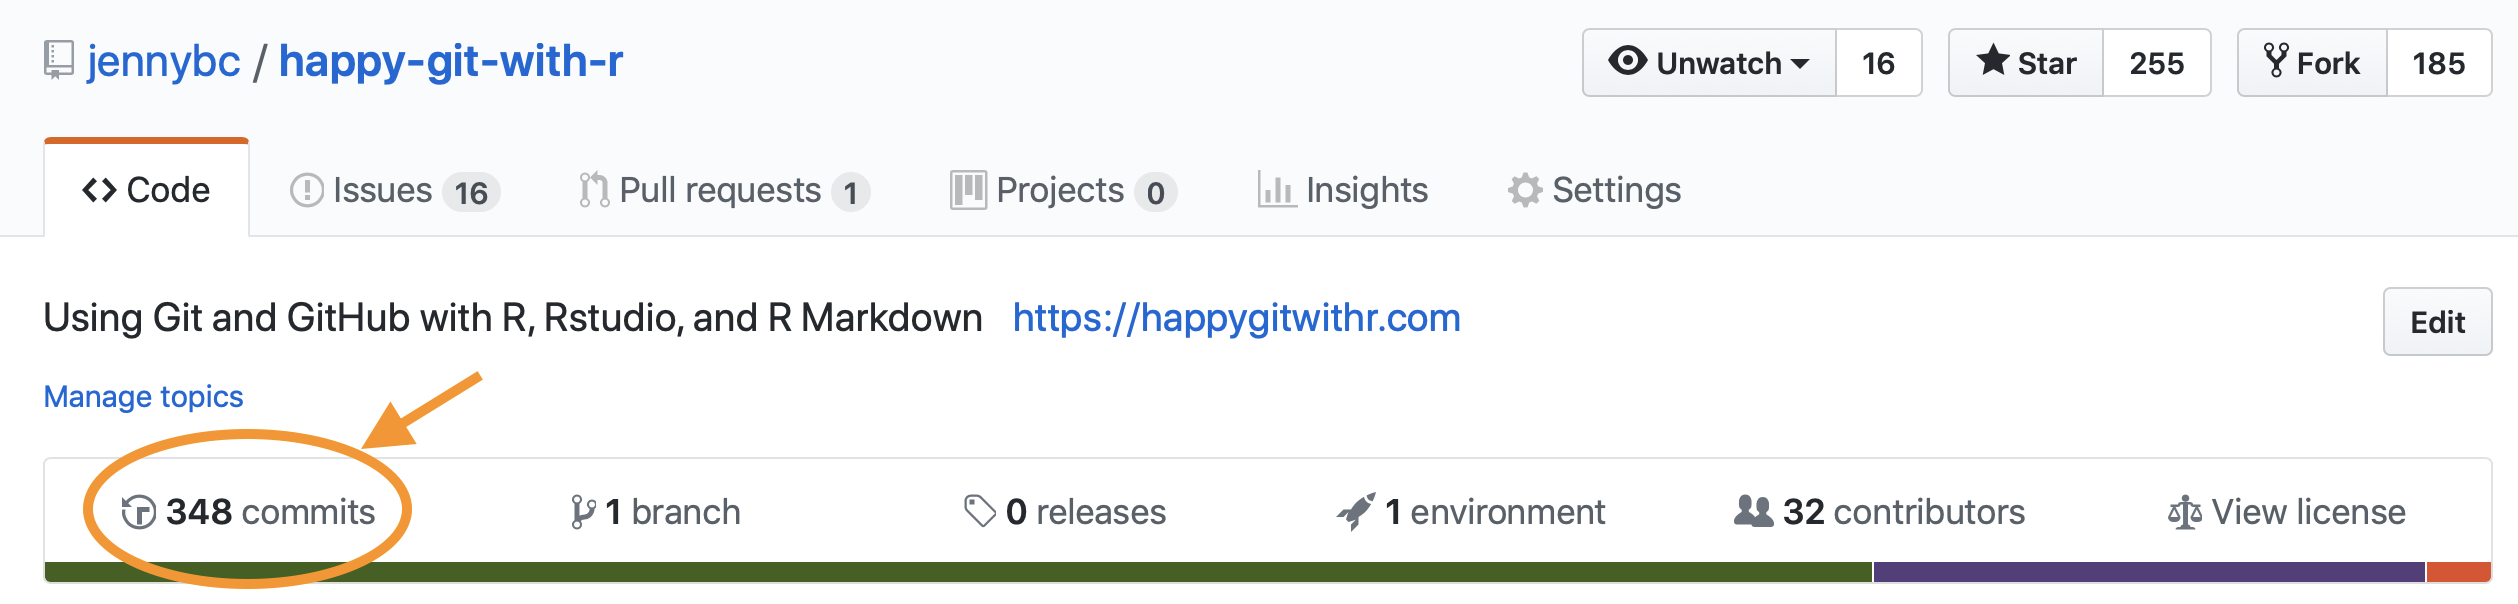
\includegraphics[width=1\linewidth]{img/screenshots/github-link-to-commits} \caption{Link to commit listing on GitHub.}\label{fig:github-link-to-commit-listing}
\end{figure}

Once you're viewing the history, notice three ways to access more info for each commit:

\begin{enumerate}
\def\labelenumi{\arabic{enumi}.}
\tightlist
\item
  The clipboard icon copies the SHA-1 of the commit. This can be handy if you need to refer to this commit elsewhere, e.g.~in an issue thread or a commit message or in a Git command you're forming for local execution.
\item
  Click on the abbreviated SHA-1 itself in order to the view the diff associated with the commit.
\item
  Click on the double angle brackets \texttt{\textless{}\textgreater{}} to browse the state of the entire repo at that point in history.
\end{enumerate}

\begin{figure}
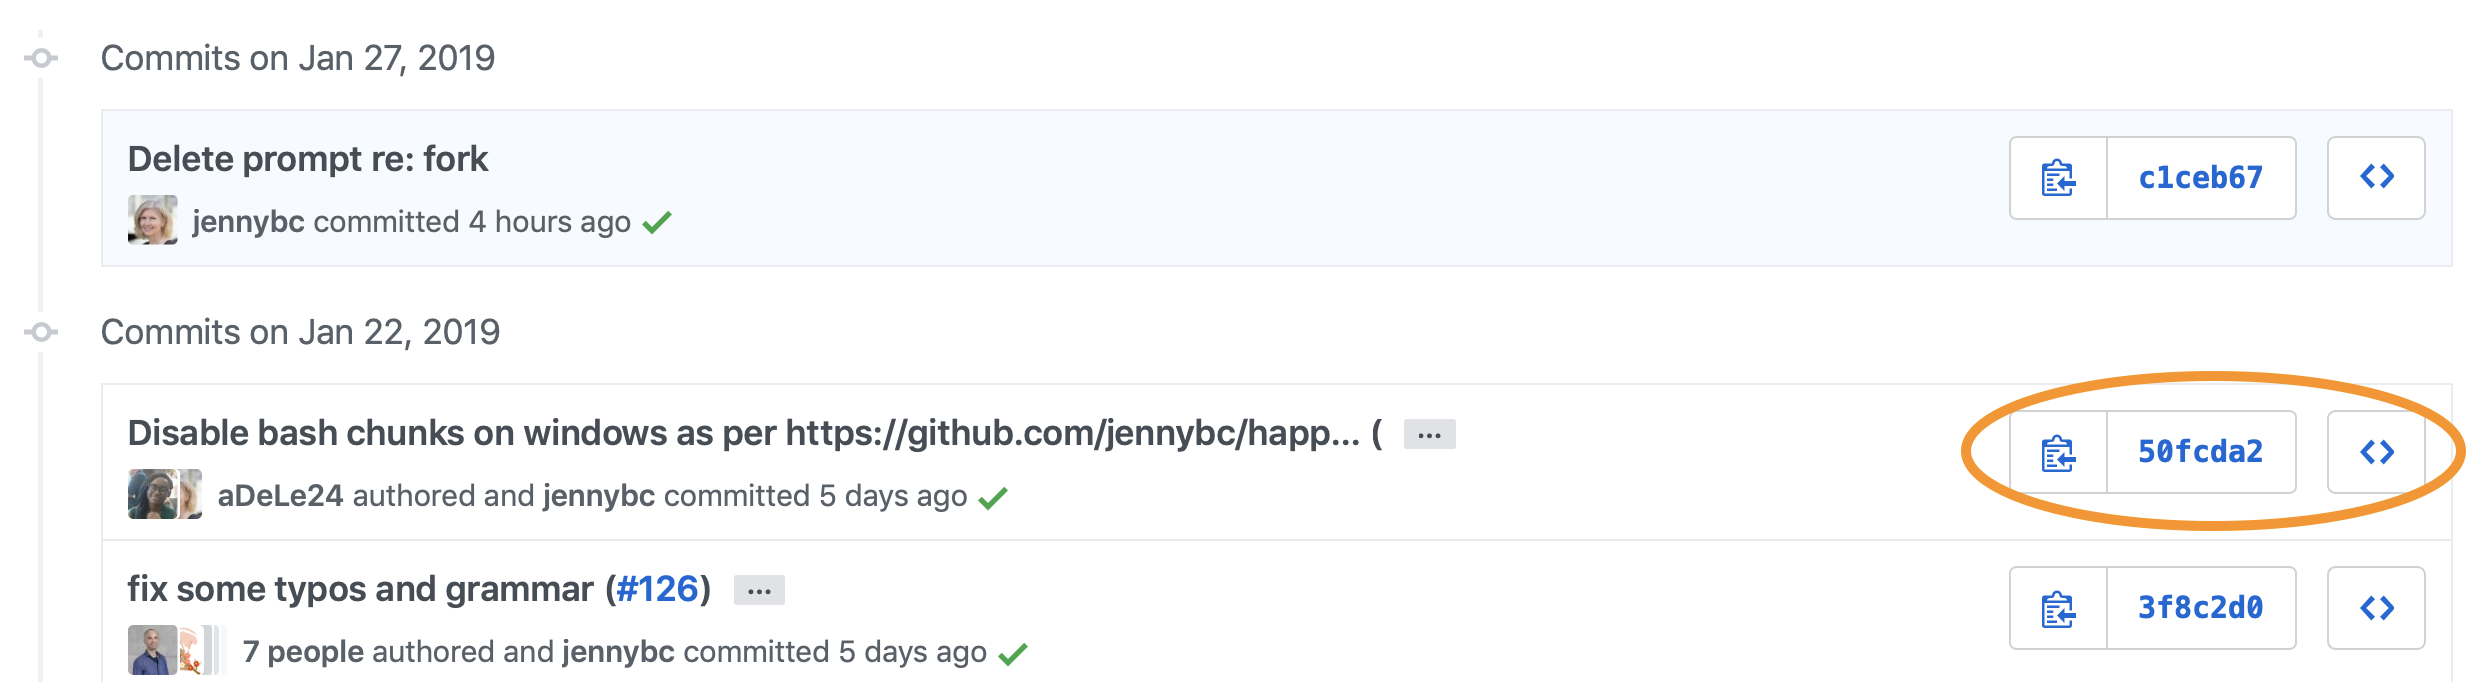
\includegraphics[width=1\linewidth]{img/screenshots/github-commit-listing} \caption{Example of a commit listing on GitHub.}\label{fig:github-commit-listing}
\end{figure}

Back out of any drilled down view by clicking on \texttt{YOU/REPO} to return to your repo's landing page. This brings you back to the present state and top-level of your repo.

\subsection{Use hyperlinks yourself!}\label{use-hyperlinks-yourself}

Once you've identified a relevant commit, diff, or file state, you can copy the current URL from your browser and use it to enhance online discussion elsewhere, i.e.~to bring other people to this exact view of the repo. The hyperlink-iness of repos hosted on GitHub can make online discussion of a project much more precise and efficient.

\section{File driven inquiries}\label{file-driven-inquiries}

What if you're interested in how a specific file came to be the way it is? First navigate to the file, then notice ``Blame'' and ``History'' in the upper right.

\begin{figure}
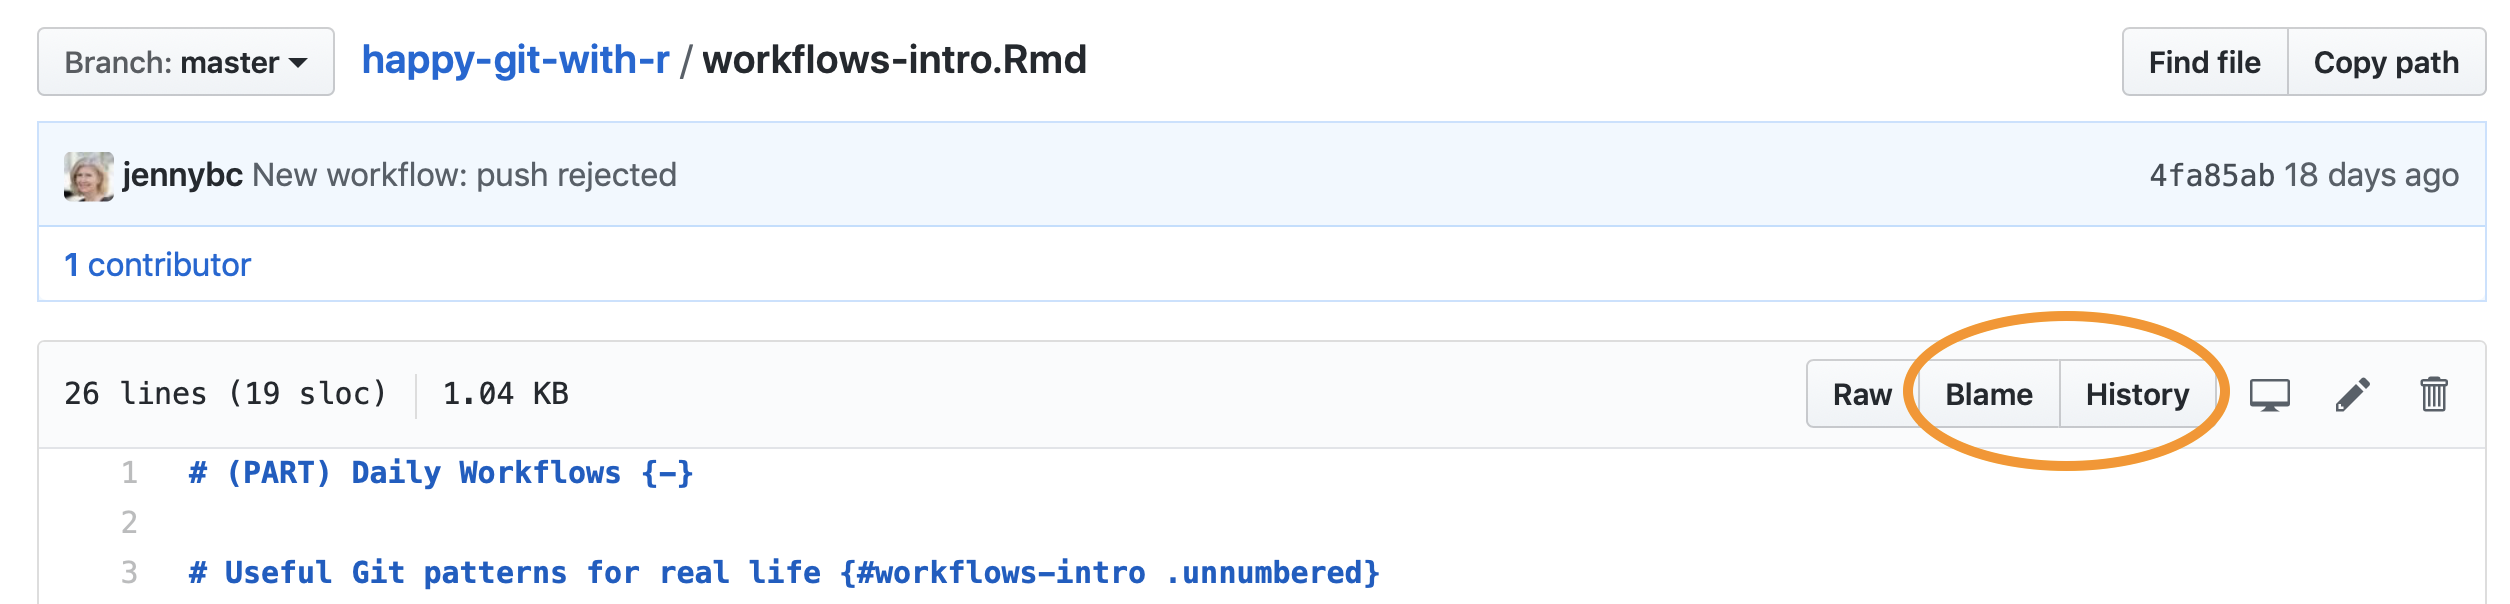
\includegraphics[width=1\linewidth]{img/screenshots/github-specific-file} \caption{Visiting a specific file on GitHub.}\label{fig:github-specific-file}
\end{figure}

\subsection{Blame}\label{blame}

The ``blame'' view of a file is related to what \texttt{git\ blame} does on the command line. It reveals who last touched each line of the file, how long ago, and the associated commit message. Click on the commit message to visit that commit. Or click the ``stacked rectangles'' icon to move further back in time, but staying in blame view. This is handy when doing forensics on a specific and small set of lines.

\emph{add a screenshot (and update that above) but first pick a better example than Happy Git, i.e.~one with more contributors / more interesting history}

\subsection{History}\label{history}

The ``history'' view for a file is very much like the overall commit history described above, except it only includes commits that affect the file of interest. This can be handy when your inquiry is rather diffuse and you're trying to digest the general story arc for a file.

\subsection{Hyperlink to specific lines at a specific state}\label{hyperlink-to-specific-lines-at-a-specific-state}

When viewing a file on GitHub, you can click on a line number to highlight it. Use ``click \ldots{} shift-click'' to select a range of lines. Notice your browser's URL shows something of this form:

\begin{Shaded}
\begin{Highlighting}[]
\ExtensionTok{https://github.com/OWNER/REPO/blob/SHA/path/to/file.R\#L27{-}L31}
\end{Highlighting}
\end{Shaded}

If the URL does not contain the SHA, type ``y'' to toggle into that form.

These file- and SHA-specific URLs are a great way to point people at particular lines of code in online conversations. It's best practice to use the uglier links that contain the SHA, as they will stand the test of time.

\section{Search}\label{search}

Search is always available in the upper-righthand corner of GitHub.

\begin{figure}
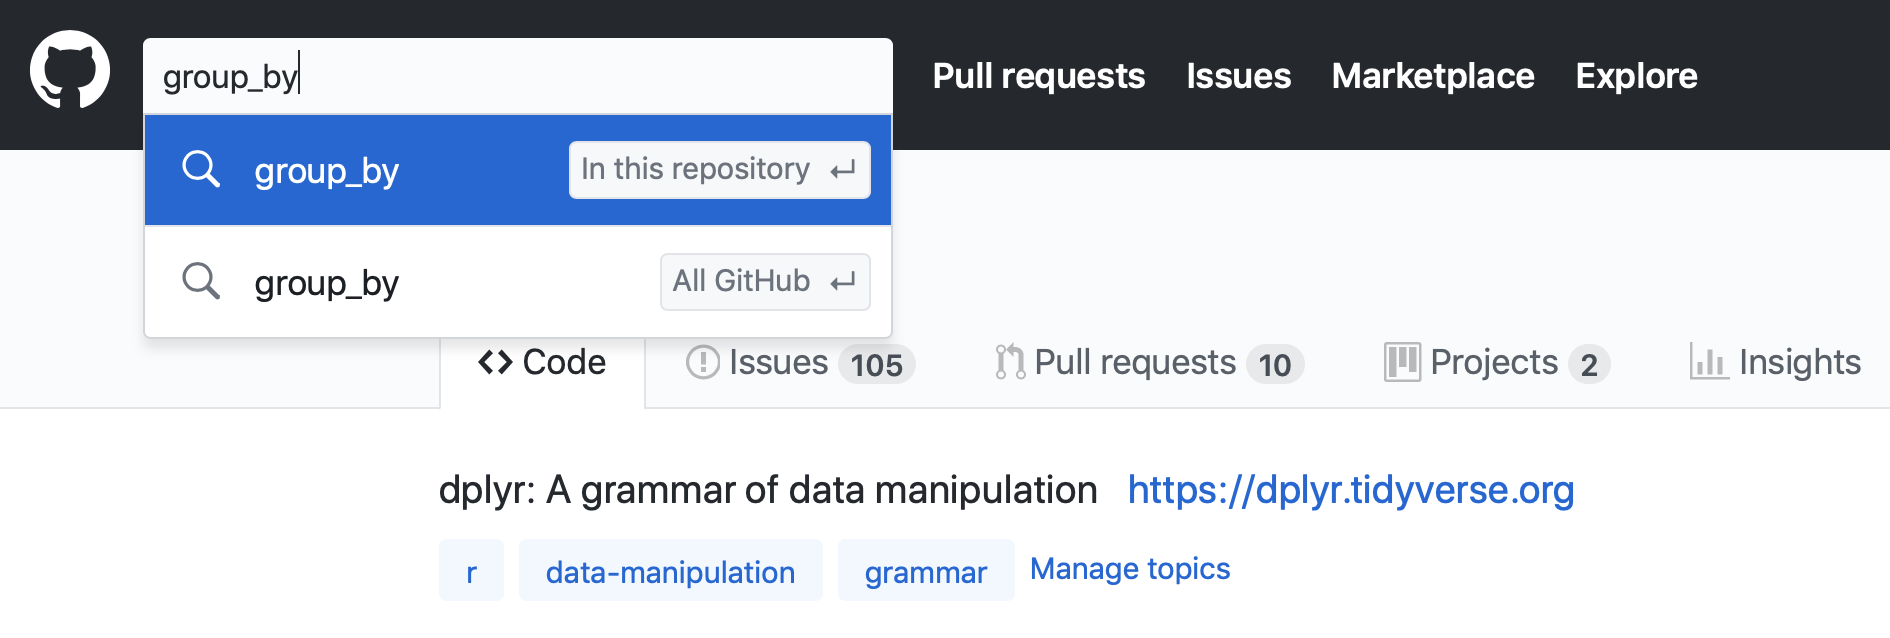
\includegraphics[width=1\linewidth]{img/screenshots/github-repo-search} \caption{Typing into GitHub search bar.}\label{fig:github-repo-search}
\end{figure}

Once you enter some text in the search box, a dropdown provides the choice to search in the current repo (the default) or all of GitHub. GitHub searches the contents of files (described as ``Code''), commit messages, and issues. Take advantage of the search hits across these different domains. Again, this is a powerful way to zoom in on specific lines of code, revisit an interesting time in project history, or re-discover a conversation thread.

\subsection{Issue search}\label{issue-search}

If you want to search issues specifically, the search box on any repo's Issues page is prepopulated with the filters \texttt{is:issue} and \texttt{is:open}.

\chapter{Fork and clone}\label{fork-and-clone}

Use \textbf{fork and clone} to get a copy of someone else's repo if there's any chance you will want to propose a change to the owner, i.e.~send a pull request.
If you are waffling between ``just clone'' and ``fork and clone'', go with ``fork and clone''.

We want to achieve this:

\begin{center}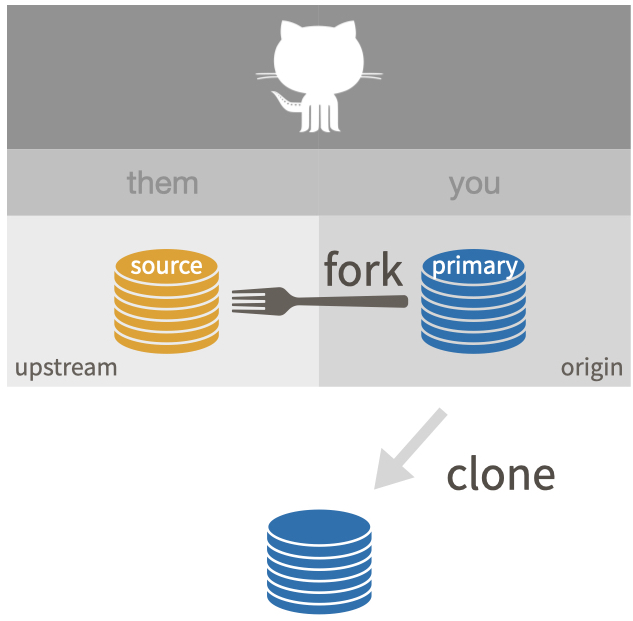
\includegraphics[width=0.6\linewidth]{img/fork-and-clone} \end{center}

Below we show a couple of methods for fork and clone and you should pick one:

\begin{itemize}
\tightlist
\item
  Use a combination of the browser, command line Git, and RStudio
\item
  Via \texttt{usethis::create\_from\_github()}
\end{itemize}

Vocabulary: \texttt{OWNER/REPO} refers to what we call the \textbf{source} repo, owned by \texttt{OWNER}, who is not you.
\texttt{YOU/REPO} refers to your fork, i.e.~your remote copy of the source repo, on GitHub.
This is the same vocabulary used elsewhere, such as the chapter on \hyperref[common-remote-setups]{common remote configurations}.

This is a good time to navigate to the \href{https://github.com}{GitHub} repo of interest, i.e.~the source repo \texttt{OWNER/REPO}.

\section{Fork and clone without usethis}\label{fork-and-clone-without-usethis}

I assume you're already visiting the source repo in the browser.
In the upper right hand corner, click \textbf{Fork}.

This creates a copy of \texttt{REPO} in your GitHub account and takes you there in the browser.
Now we are looking at \texttt{YOU/REPO}.

\textbf{Clone} \texttt{YOU/REPO}, which is your copy of the repo, a.k.a. your fork, to your local machine.
Make sure to clone your repo, not the source repo.
Elsewhere, we describe multiple methods for cloning a remote repo.
Pick one:

\begin{itemize}
\tightlist
\item
  The \hyperref[git-clone-usethis-rstudio]{cloning instructions in Existing project, GitHub first}
  cover usethis and RStudio.
\item
  The \hyperref[git-clone-command-line]{cloning instructions in Connect to GitHub}
  show how to do this with command line Git.
\end{itemize}

Make a conscious decision about the local destination directory and HTTPS vs SSH URL.

\subsection{Finish the fork and clone setup}\label{fork-and-clone-finish}

If you stop at this point, you have what I regard as an incomplete setup, described elsewhere as \hyperref[fork_upstream_is_not_origin_parent]{``fork (salvageable)''}.

\begin{center}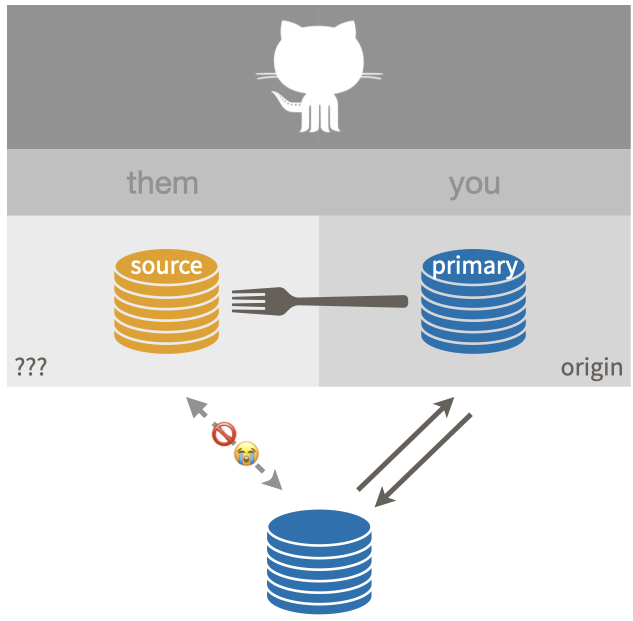
\includegraphics[width=0.6\linewidth]{img/fork-no-upstream-sad} \end{center}

This is sad, because there is no direct connection between your local copy of the repo and the source repo \texttt{OWNER/REPO}.

There are two more recommended pieces of setup:

\begin{itemize}
\tightlist
\item
  Configure the source repo as the \texttt{upstream} remote
\item
  Configure your local \texttt{main} branch (or whatever the default is) to track
  \texttt{upstream/main}, not \texttt{origin/main}
\end{itemize}

The nickname \texttt{upstream} can technically be whatever you want.
There is a strong tradition of using \texttt{upstream} in this context and, even though I have better ideas, I believe it is best to conform.
Every book, blog post, and Stack Overflow thread that you read will use \texttt{upstream} here.
Save your psychic energy for other things.

These steps make it easier for you to stay current with developments in the source repo.
We talk more below about why you should never commit to the default branch, e.g.~\texttt{main}, when you're working in a fork (see \ref{fork-dont-touch-main}).

\subsection{\texorpdfstring{Configure the \texttt{upstream} remote}{Configure the upstream remote}}\label{fork-configure-upstream}

The first step is to get the URL of the \textbf{source} repo \texttt{OWNER/REPO}.
Navigate to the source repo on GitHub.
It is easy to get to from your fork, \texttt{YOU/REPO}, via the ``forked from'' link in the upper left.

Use the big green ``Code'' button to get the URL for \texttt{OWNER/REPO} on your clipboard.
Be intentional about whether you copy the HTTPS or SSH URL.

You can configure the \texttt{upstream} remote with command line Git, usethis, or RStudio.

Here's how to use command line Git in a shell:

\begin{Shaded}
\begin{Highlighting}[]
\FunctionTok{git}\NormalTok{ remote add upstream https://github.com/OWNER/REPO.git}
\end{Highlighting}
\end{Shaded}

\texttt{usethis::use\_git\_remote()} allows you to configure a Git remote.
Execute this in R:

\begin{Shaded}
\begin{Highlighting}[]
\NormalTok{usethis}\SpecialCharTok{::}\FunctionTok{use\_git\_remote}\NormalTok{(}
  \AttributeTok{name =} \StringTok{"upstream"}\NormalTok{,}
  \AttributeTok{url =} \StringTok{"https://github.com/OWNER/REPO.git"}
\NormalTok{)}
\end{Highlighting}
\end{Shaded}

Finally, you can do this in RStudio, although it feels a bit odd.
Click on ``New Branch'' in the Git pane (``two purple boxes and a white square'').

\begin{center}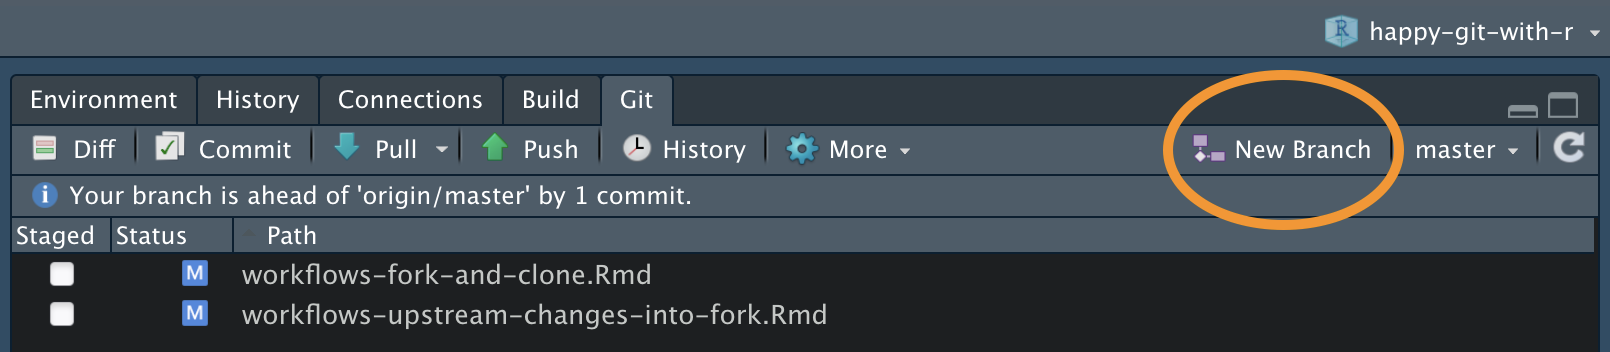
\includegraphics[width=0.6\linewidth]{img/rstudio-new-branch} \end{center}

This will reveal a button to ``Add Remote''.
Click it.
Enter \texttt{upstream} as the remote name and paste the URL for \texttt{OWNER/REPO} that you got from GitHub.
Click ``Add''.
Decline the opportunity to add a new branch by clicking ``Cancel''.

Regardless of how you configured \texttt{upstream}, do this in a shell:

\begin{Shaded}
\begin{Highlighting}[]
\FunctionTok{git}\NormalTok{ fetch upstream}
\end{Highlighting}
\end{Shaded}

\subsection{Set upstream tracking branch for the default branch}\label{fork-set-upstream-tracking-main}

This is optional but highly recommended for most fork and clone situations.
We're going to set \texttt{upstream/main} from the source repo as the upstream tracking branch of local \texttt{main}.
(If your default branch has a different name, substitute accordingly.)

This is desirable so that a simple \texttt{git\ pull} pulls \textbf{from the source repo}, not from your fork.
It also means a simple \texttt{git\ push} will (attempt to) push to the source repo, which will almost always be rejected since you probably do not have permission.
This failure will alert you to the fact that you're doing something questionable, while it's still easy to back out.

First, fetch info for the \texttt{upstream} remote.
This is especially important if you just configured \texttt{upstream} for the first time.

\begin{Shaded}
\begin{Highlighting}[]
\FunctionTok{git}\NormalTok{ fetch upstream}
\end{Highlighting}
\end{Shaded}

The two commands below do the same thing; the first is just shorthand for the second.
Do this with command line Git in a shell:

\begin{Shaded}
\begin{Highlighting}[]
\FunctionTok{git}\NormalTok{ branch }\AttributeTok{{-}u}\NormalTok{ upstream/main}
\FunctionTok{git}\NormalTok{ branch }\AttributeTok{{-}{-}set{-}upstream{-}to}\NormalTok{ upstream/main}
\end{Highlighting}
\end{Shaded}

If you found this fork and clone workflow long and tedious, consider using \texttt{usethis::create\_from\_github()} next time!

\section{\texorpdfstring{\texttt{usethis::create\_from\_github("OWNER/REPO",\ fork\ =\ TRUE)}}{usethis::create\_from\_github("OWNER/REPO", fork = TRUE)}}\label{fork-and-clone-create-from-github}

The \href{https://usethis.r-lib.org}{usethis package} has a convenience function, \href{https://usethis.r-lib.org/reference/create_from_github.html}{\texttt{create\_from\_github()}}, that can do ``fork and clone'' (as well as just clone).
The \texttt{fork} argument controls whether the source repo is cloned or fork-and-cloned.
Note that \texttt{create\_from\_github(fork\ =\ TRUE)} requires that you have \hyperref[https-pat]{configured a GitHub personal access token}.

I assume you're already visiting the source repo in the browser.
Now click the big green button that says ``\textless\textgreater{} Code''.
Copy a clone URL to your clipboard.
If you're taking our default advice, copy the HTTPS URL.
But if you're opting for SSH, then make sure to copy the SSH URL.

You can execute this next command in any R session.
If you use RStudio, then do this in the R console of any RStudio instance.
In either case, after successful completion, you should find yourself in the new project that is the local repo connected to your fork.

\begin{Shaded}
\begin{Highlighting}[]
\NormalTok{usethis}\SpecialCharTok{::}\FunctionTok{create\_from\_github}\NormalTok{(}
  \StringTok{"https://github.com/OWNER/REPO"}\NormalTok{,}
  \AttributeTok{destdir =} \StringTok{"\textasciitilde{}/path/to/where/you/want/the/local/repo/"}\NormalTok{,}
  \AttributeTok{fork =} \ConstantTok{TRUE}
\NormalTok{)}
\end{Highlighting}
\end{Shaded}

The first argument is \texttt{repo\_spec} and it accepts the GitHub repo specification in various forms.
In particular, you can use the URL we just copied for the source repo.

The \texttt{destdir} argument specifies the parent directory where you want the new folder (and local Git repo) to live.
If you don't specify \texttt{destdir}, usethis defaults to some very conspicuous place, like your desktop.
If you like to keep Git repos in a certain folder on your computer, you can personalize this default by setting the \texttt{usethis.destdir} option in your \texttt{.Rprofile}.

The \texttt{fork} argument specifies whether to clone (\texttt{fork\ =\ FALSE}) or fork and clone (\texttt{fork\ =\ TRUE}).
You often don't need to specify \texttt{fork} and can just enjoy the default behaviour, which is governed by your permissions on the source repo.
By default, \texttt{fork\ =\ FALSE} if you can push to the source repo and \texttt{fork\ =\ TRUE} if you cannot.

Here is what that might look like (note that we're accepting the default behaviour for many arguments):

\begin{Shaded}
\begin{Highlighting}[]
\NormalTok{usethis}\SpecialCharTok{::}\FunctionTok{create\_from\_github}\NormalTok{(}\StringTok{"https://github.com/OWNER/REPO"}\NormalTok{)}
\CommentTok{\#\textgreater{} ℹ Defaulting to \textquotesingle{}https\textquotesingle{} Git protocol}
\CommentTok{\#\textgreater{} ✔ Setting \textasciigrave{}fork = TRUE\textasciigrave{}}
\CommentTok{\#\textgreater{} ✔ Creating \textquotesingle{}/some/path/to/local/REPO/\textquotesingle{}}
\CommentTok{\#\textgreater{} ✔ Forking \textquotesingle{}OWNER/REPO\textquotesingle{}}
\CommentTok{\#\textgreater{} ✔ Cloning repo from \textquotesingle{}https://github.com/YOU/REPO.git\textquotesingle{} into \textquotesingle{}/some/path/to/local/REPO\textquotesingle{}}
\CommentTok{\#\textgreater{} ✔ Setting active project to \textquotesingle{}/some/path/to/local/REPO\textquotesingle{}}
\CommentTok{\#\textgreater{} ℹ Default branch is \textquotesingle{}main\textquotesingle{}}
\CommentTok{\#\textgreater{} ✔ Adding \textquotesingle{}upstream\textquotesingle{} remote: \textquotesingle{}https://github.com/OWNER/REPO.git\textquotesingle{}}
\CommentTok{\#\textgreater{} ✔ Pulling changes from \textquotesingle{}upstream/main\textquotesingle{}.}
\CommentTok{\#\textgreater{} ✔ Setting remote tracking branch for local \textquotesingle{}main\textquotesingle{} branch to \textquotesingle{}upstream/main\textquotesingle{}}
\CommentTok{\#\textgreater{} ✔ Setting active project to \textquotesingle{}\textless{}no active project\textgreater{}\textquotesingle{}}
\end{Highlighting}
\end{Shaded}

For an RStudio user, \texttt{create\_from\_github(fork\ =\ TRUE)} does all of this:

\begin{itemize}
\tightlist
\item
  Forks the source repo on GitHub.
\item
  Clones your fork to a new local repo (and RStudio Project).
  This configures your fork as the \texttt{origin} remote.
\item
  Configures the source repo as \hyperref[upstream-changes]{the \texttt{upstream} remote}.
\item
  Sets the upstream tracking branch for \texttt{main} (or whatever the default branch
  is) to \texttt{upstream/main}.
\item
  Opens a new RStudio instance in the new local repo (and RStudio Project).
\end{itemize}

\section{Engage with the new repo}\label{engage-with-the-new-repo}

If you used \texttt{usethis::create\_from\_github()} or did fork and clone via \hyperref[existing-github-first]{Existing project, GitHub first}, you are probably in an RStudio Project for this new repo.

Regardless, get yourself into this project, whatever that means for you, using your usual method.

Explore the new repo in some suitable way.
If it is a package, you could run the tests or check it.
If it is a data analysis project, run a script or render an Rmd.
Convince yourself that you have gotten the code.

You should now be in the perfect position to sync up with ongoing developments in the source repo and to propose new changes via a pull request from your fork.

\begin{center}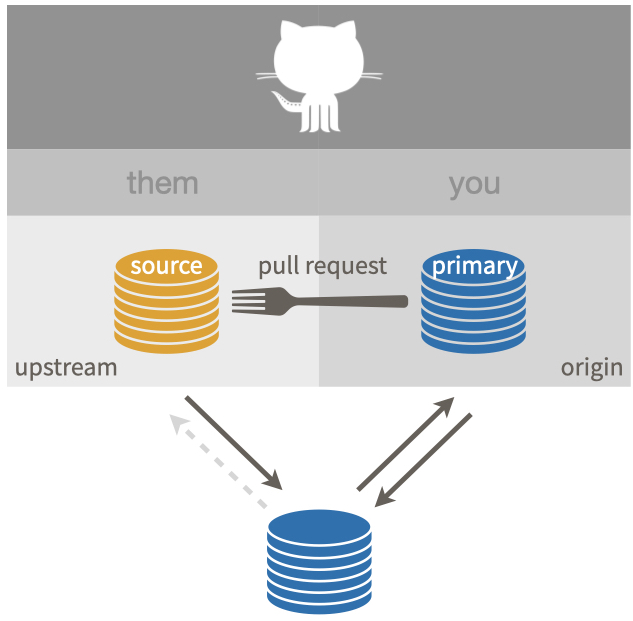
\includegraphics[width=0.6\linewidth]{img/fork-them-pull-request} \end{center}

You can use the commands below to review more of the nitty gritty Git details of your fork and clone setup:

\begin{itemize}
\tightlist
\item
  Command line Git in a shell:

  \begin{itemize}
  \tightlist
  \item
    \texttt{git\ remote\ -v}
  \item
    \texttt{git\ remote\ show\ origin} (or \texttt{upstream})
  \item
    \texttt{git\ branch\ -vv}
  \end{itemize}
\item
  In R:

  \begin{itemize}
  \tightlist
  \item
    \texttt{usethis::git\_remotes()}
  \item
    \texttt{usethis::git\_sitrep()}
  \end{itemize}
\end{itemize}

In the shell, \texttt{git\ remote\ -v} should reveal that your remotes are configured like so:

\begin{Shaded}
\begin{Highlighting}[]
\ExtensionTok{origin}\NormalTok{    https://github.com/YOU/REPO.git }\ErrorTok{(}\ExtensionTok{fetch}\KeywordTok{)}
\ExtensionTok{origin}\NormalTok{    https://github.com/YOU/REPO.git }\ErrorTok{(}\ExtensionTok{push}\KeywordTok{)}
\ExtensionTok{upstream}\NormalTok{  https://github.com/OWNER/REPO.git }\ErrorTok{(}\ExtensionTok{fetch}\KeywordTok{)}
\ExtensionTok{upstream}\NormalTok{  https://github.com/OWNER/REPO.git }\ErrorTok{(}\ExtensionTok{push}\KeywordTok{)}
\end{Highlighting}
\end{Shaded}

Comparable info is available In R with \texttt{usethis::git\_remotes()}:

\begin{Shaded}
\begin{Highlighting}[]
\FunctionTok{git\_remotes}\NormalTok{()}
\CommentTok{\#\textgreater{} $origin}
\CommentTok{\#\textgreater{} [1] "https://github.com/YOU/REPO.git"}
\CommentTok{\#\textgreater{} }
\CommentTok{\#\textgreater{} $upstream}
\CommentTok{\#\textgreater{} [1] "https://github.com/OWNER/repo.git"}
\end{Highlighting}
\end{Shaded}

In the shell, with the default branch checked out, \texttt{git\ branch\ -vv} should reveal that \texttt{upstream/main} is the upstream tracking branch:

\begin{Shaded}
\begin{Highlighting}[]
\ExtensionTok{\textasciitilde{}/some/repo/}\NormalTok{ \% git branch }\AttributeTok{{-}vv}                   
\ExtensionTok{*}\NormalTok{ main 2739987 }\PreprocessorTok{[}\SpecialStringTok{upstream/main}\PreprocessorTok{]}\NormalTok{ Some commit message}
\end{Highlighting}
\end{Shaded}

All of this info about remotes and branches is also included in the rich information reported with \texttt{usethis::git\_sitrep()}.

\section{\texorpdfstring{Don't mess with \texttt{main}}{Don't mess with main}}\label{fork-dont-touch-main}

Here is some parting advice for how to work in a fork and clone and situation.

If you make any commits in your local repository, I \textbf{strongly recommend} that you work in \hyperref[git-branches]{a new branch}, not \texttt{main} (or whatever the default branch is called).

I \textbf{strongly recommend} that you do not make commits to \texttt{main} of a repo you have forked.
If you commit to \texttt{main} in a repo you don't own, it creates a divergence between that branch's history in the source repo and in your repo.
Nothing but pain will come from this.
(If you've already done this, we discuss how to fix the situation in \hyperref[touched-main]{Um, what if I did touch \texttt{main}?}.)

When you treat \texttt{main} as read-only, it makes life much easier when you want to \hyperref[upstream-changes]{pull upstream work} into your copy.
The \texttt{OWNER} of \texttt{REPO} will also be happier to receive your pull request from a non-\texttt{main} branch.

For more detail, this Q\&A on Stack Overflow is helpful: \href{https://stackoverflow.com/q/33749832}{Why is it bad practice to commit to your fork's master branch?}.

\chapter{Get upstream changes for a fork}\label{upstream-changes}

This workflow is relevant if you have done \hyperref[fork-and-clone]{fork and clone} and now you need to pull subsequent changes from the source repo into your copy.
We are talking about both your fork (your remote copy of the repo, on GitHub) and your local copy.

This is the ideal starting situation:

\begin{center}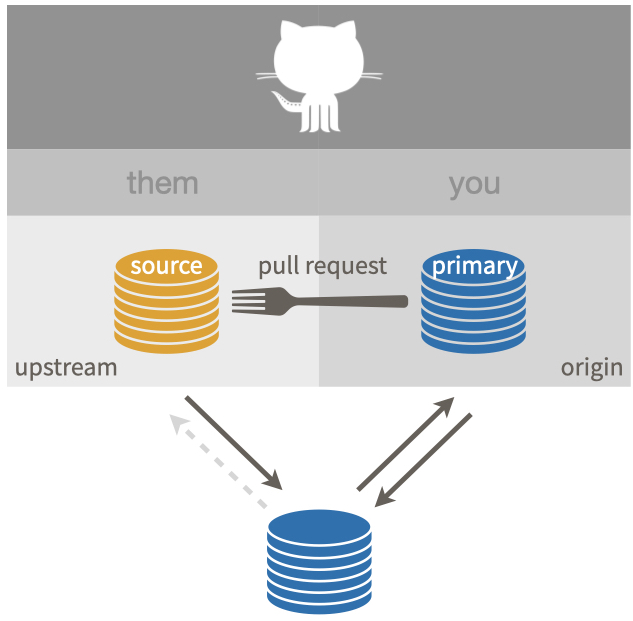
\includegraphics[width=0.6\linewidth]{img/fork-them-pull-request} \end{center}

First, we're going to actively verify the above configuration.
If your setup is sub-optimal, we'll discuss how to address that.

\section{Verify your local repo's configuration}\label{verify-your-local-repos-configuration}

Vocabulary: \texttt{OWNER/REPO} refers to what we call the \textbf{source} repo, owned by \texttt{OWNER}, who is not you.
\texttt{YOU/REPO} refers to your fork, i.e.~your remote copy of the source repo, on GitHub.
This is the same vocabulary used elsewhere, such as the chapter on \hyperref[common-remote-setups]{common remote configurations}.

\subsection{List your remotes}\label{list-your-remotes}

Let's inspect \hyperref[git-remotes]{the current remotes} for your local repo.

You can check this with command line Git in the shell (Appendix \ref{shell}):

\begin{Shaded}
\begin{Highlighting}[]
\FunctionTok{git}\NormalTok{ remote }\AttributeTok{{-}v}
\end{Highlighting}
\end{Shaded}

We want to see something like this:

\begin{Shaded}
\begin{Highlighting}[]
\ExtensionTok{origin}\NormalTok{    https://github.com/YOU/REPO.git }\ErrorTok{(}\ExtensionTok{fetch}\KeywordTok{)}
\ExtensionTok{origin}\NormalTok{    https://github.com/YOU/REPO.git }\ErrorTok{(}\ExtensionTok{push}\KeywordTok{)}
\ExtensionTok{upstream}\NormalTok{  https://github.com/OWNER/REPO.git }\ErrorTok{(}\ExtensionTok{fetch}\KeywordTok{)}
\ExtensionTok{upstream}\NormalTok{  https://github.com/OWNER/REPO.git }\ErrorTok{(}\ExtensionTok{push}\KeywordTok{)}
\end{Highlighting}
\end{Shaded}

Comparable info is available in R with \texttt{usethis::git\_remotes()}:

\begin{Shaded}
\begin{Highlighting}[]
\FunctionTok{git\_remotes}\NormalTok{()}
\CommentTok{\#\textgreater{} $origin}
\CommentTok{\#\textgreater{} [1] "https://github.com/YOU/REPO.git"}
\CommentTok{\#\textgreater{} }
\CommentTok{\#\textgreater{} $upstream}
\CommentTok{\#\textgreater{} [1] "https://github.com/OWNER/repo.git"}
\end{Highlighting}
\end{Shaded}

If you only have one remote, probably \texttt{origin}, I highly recommend you modify the remote configuration.
But first, we'll check one other thing.

\subsection{View the upstream tracking branch}\label{view-the-upstream-tracking-branch}

Ideally, your local \texttt{main} branch has \texttt{upstream/main} as its upstream tracking branch.
Even you have a correctly configured \texttt{upstream} remote, this is worth checking.
If your default branch has a branch other than \texttt{main}, substitute accordingly.

In the shell, with the default branch checked out, \texttt{git\ branch\ -vv} should reveal that \texttt{upstream/main} is the upstream tracking branch:

\begin{Shaded}
\begin{Highlighting}[]
\ExtensionTok{\textasciitilde{}/some/repo/}\NormalTok{ \% git branch }\AttributeTok{{-}vv}                   
\ExtensionTok{*}\NormalTok{ main 2739987 }\PreprocessorTok{[}\SpecialStringTok{upstream/main}\PreprocessorTok{]}\NormalTok{ Some commit message}
\end{Highlighting}
\end{Shaded}

If, instead, you see \texttt{origin/main}, I highly recommend you reconfigure the tracking branch.

All of this info about remotes and branches is also included in the rich information reported with \texttt{usethis::git\_sitrep()}.

\subsection{Repair or complete your repo's configuration}\label{repair-or-complete-your-repos-configuration}

Instructions for adding the \texttt{upstream} remote and setting upstream tracking for your default branch are given in \hyperref[fork-and-clone-finish]{Finish the fork and clone setup}.

\section{Verify that your ``working tree is clean''}\label{verify-that-your-working-tree-is-clean}

We assume your repo has this favorable configuration:

\begin{center}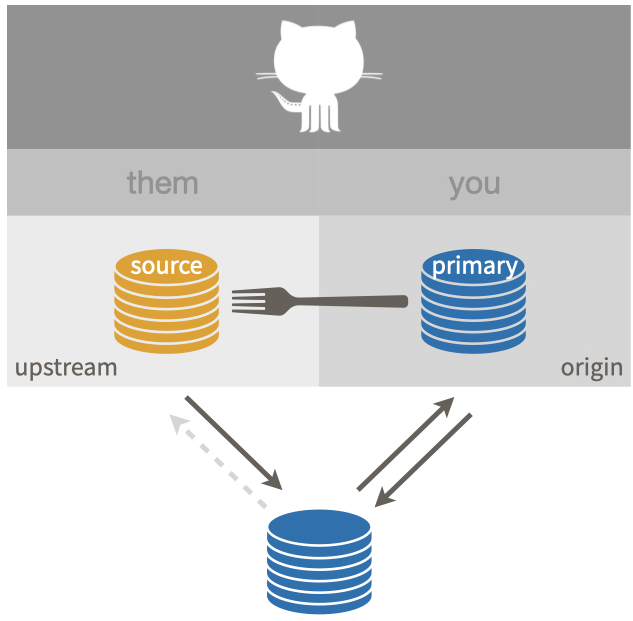
\includegraphics[width=0.6\linewidth]{img/fork-them} \end{center}

Make sure you are on the default branch, e.g.~\texttt{main}, and that your ``working tree is clean''.
First, let's make sure our information on the \texttt{upstream} remote is current:

\begin{Shaded}
\begin{Highlighting}[]
\FunctionTok{git}\NormalTok{ fetch upstream}
\end{Highlighting}
\end{Shaded}

\texttt{git\ status} should now show something like:

\begin{Shaded}
\begin{Highlighting}[]
\ExtensionTok{On}\NormalTok{ branch main}
\ExtensionTok{Your}\NormalTok{ branch is up to date with }\StringTok{\textquotesingle{}origin/main\textquotesingle{}}\NormalTok{.}

\ExtensionTok{nothing}\NormalTok{ to commit, working tree clean}
\end{Highlighting}
\end{Shaded}

If you have modified files, you should either discard those changes or create a new branch and commit the changes there for safekeeping.

It's also fine if you see something like this:

\begin{verbatim}
Your branch is behind 'upstream/main' by 2 commits, and can be fast-forwarded.
\end{verbatim}

However, if you see something like this:

\begin{verbatim}
Your branch is ahead of 'upstream/main' by 1 commit.
\end{verbatim}

or this:

\begin{verbatim}
Your branch and 'upstream/main' have diverged,
and have 1 and 1 different commits each, respectively.
\end{verbatim}

this is a sign that you have made some regrettable choices.

I recommend that you \hyperref[fork-dont-touch-main]{never make your own commits to the default branch of a fork} or to any branch that you don't effectively (co-)own.
However, if you have already done so, we explain how to fix the problem in \hyperref[touched-main]{Um, what if I did touch \texttt{main}?}.

\section{\texorpdfstring{Sync option 1: Pull changes from \texttt{upstream}, then push to \texttt{origin}}{Sync option 1: Pull changes from upstream, then push to origin}}\label{sync-option-1-pull-changes-from-upstream-then-push-to-origin}

Now we are ready to pull the changes that we don't have from the source repo \texttt{OWNER/REPO} into our local copy.

\begin{Shaded}
\begin{Highlighting}[]
\FunctionTok{git}\NormalTok{ pull upstream main }\AttributeTok{{-}{-}ff{-}only}
\end{Highlighting}
\end{Shaded}

This says: ``pull the changes from the remote known as \texttt{upstream} into the \texttt{main} branch of my local repo''.
I am being explicit about the remote (\texttt{upstream}) and the branch (\texttt{main}) in this case, both to make it more clear and to make this command robust to repo- and user-level Git configurations.
But if you've followed our setup recommendations, you don't actually need to be this explicit.

I also \textbf{highly recommend} using the \texttt{-\/-ff-only} flag in this case, so that you also say ``if I have made my own commits to \texttt{main}, please force me to confront this problem NOW''.
Here's what it looks like if a fast-forward merge isn't possible:

\begin{Shaded}
\begin{Highlighting}[]
\ExtensionTok{$}\NormalTok{ git pull upstream main }\AttributeTok{{-}{-}ff{-}only}
\ExtensionTok{From}\NormalTok{ github.com:OWNER/REPO}
 \ExtensionTok{*}\NormalTok{ branch              main     }\AttributeTok{{-}}\OperatorTok{\textgreater{}}\NormalTok{ FETCH\_HEAD}
\ExtensionTok{fatal:}\NormalTok{ Not possible to fast{-}forward, aborting.}
\end{Highlighting}
\end{Shaded}

See \hyperref[touched-main]{Um, what if I did touch \texttt{main}?} to get yourself back on the happy path.

Assuming you've succeeded with \texttt{git\ pull}, this next step is optional and many people who are facile with Git do not bother.

If you take my advice to \hyperref[fork-dont-touch-main]{never work in \texttt{main} of a fork}, then the state of the \texttt{main} branch in your fork \texttt{YOU/REPO} does not technically matter.
You will never make a pull request from \texttt{main} and there are ways to set the correct base for the branches and pull requests that you do create.

If, however, your grasp of all these Git concepts is tenuous at best, it can be helpful to try to keep things simple and orderly and synced up.

Feel free to push the newly updated state of local \texttt{main} to your fork \texttt{YOU/REPO} and enjoy the satisfaction of being ``caught up'' with \texttt{OWNER/REPO}, in both your remote fork and in your local repo.

In the shell:

\begin{Shaded}
\begin{Highlighting}[]
\FunctionTok{git}\NormalTok{ push origin main}
\end{Highlighting}
\end{Shaded}

If you've followed our configuration advice, you really do need to be this explicit in order to push to \texttt{origin} (not \texttt{upstream}).

\section{\texorpdfstring{Sync option 2: Sync your fork on GitHub, pull changes from \texttt{origin} to local repo}{Sync option 2: Sync your fork on GitHub, pull changes from origin to local repo}}\label{sync-option-2-sync-your-fork-on-github-pull-changes-from-origin-to-local-repo}

For many years, this was not possible, though many GitHub users wished for this feature.
Happily it is now possible to sync a fork with its source repo in the browser, i.e.~to do the sync between the 2 GitHub repos.
The official GitHub documentation for this is \href{https://docs.github.com/en/pull-requests/collaborating-with-pull-requests/working-with-forks/syncing-a-fork\#syncing-a-fork-branch-from-the-web-ui}{Syncing a fork branch from the web UI}.

Navigate to the main page of your fork \texttt{YOU/REPO}, i.e.~your primary repo which is configured as the \texttt{origin} remote.

At the top you'll see some information on how the state of \texttt{main} in your fork relates to \texttt{main} in the source repo, similar to what we see with \texttt{git\ status} in the alternative approach above.
Ideally you will see something like:

\begin{verbatim}
This branch is 2 commits behind OWNER:main.
\end{verbatim}

which indicates you can sync up in the ideal fast-forward sense.

If you see something like this:

\begin{verbatim}
This branch is 1 commit ahead, 2 commits behind OWNER:main.
\end{verbatim}

this is a sign that you have made some regrettable choices.

I recommend that you \hyperref[fork-dont-touch-main]{never make your own commits to the default branch of a fork} or to any branch that you don't effectively (co-)own.
However, if you have already done so, we explain how to fix the problem in \hyperref[touched-main]{Um, what if I did touch \texttt{main}?}.

Once you are ready to proceed, click ``Sync fork'' in the upper right corner.
Upon success, the main page of \texttt{YOU/REPO} shows something like

\begin{quote}
This branch is up to date with \texttt{OWNER/REPO:main}.
\end{quote}

If you have made commits on the default branch of your fork, which we \hyperref[fork-dont-touch-main]{strongly advise against}, this can result in a merge commit (or even merge conflicts).
If you are suffering due to commits you've made on \texttt{main} and it's beyond the help we describe below, consider deleting your fork and local repo and making a fresh start with \href{fork-and-clone}{Fork and clone}.
Live and learn.

Once you have successfully synced the default branch of \texttt{YOU/REPO} with the default branch of \texttt{OWNER/REPO}, you probably want to do the same for your local repo.
Since they are synced, you can pull from either \texttt{upstream} or \texttt{origin}.

In the shell, with the default branch checked out, execute one of these:

\begin{Shaded}
\begin{Highlighting}[]
\FunctionTok{git}\NormalTok{ pull upstream main }\AttributeTok{{-}{-}ff{-}only}
\FunctionTok{git}\NormalTok{ pull origin main }\AttributeTok{{-}{-}ff{-}only}
\end{Highlighting}
\end{Shaded}

If you've followed our configuration advice, you don't actually need to specify the remote and branch, because this branch is configured to pull from \texttt{upstream}.
For the same reasons as before, it's a good idea to include the \texttt{-\/-ff-only} flag.
If you have made local commits to \texttt{main}, this will surface that problem, which is solved in the next section.

\section{\texorpdfstring{Um, what if I did touch \texttt{main}?}{Um, what if I did touch main?}}\label{touched-main}

I told you not to!

But OK here we are.

Let's imagine this is the state of \texttt{main} (or whatever the default branch is called) in the source repo \texttt{OWNER/REPO}:

\begin{Shaded}
\begin{Highlighting}[]
\ExtensionTok{...} \AttributeTok{{-}{-}}\NormalTok{ A }\AttributeTok{{-}{-}}\NormalTok{ B }\AttributeTok{{-}{-}}\NormalTok{ C }\AttributeTok{{-}{-}}\NormalTok{ D }\AttributeTok{{-}{-}}\NormalTok{ E }\AttributeTok{{-}{-}}\NormalTok{ F}
\end{Highlighting}
\end{Shaded}

and and this is the state of the \texttt{main} branch in your local copy:

\begin{Shaded}
\begin{Highlighting}[]
\ExtensionTok{...} \AttributeTok{{-}{-}}\NormalTok{ A }\AttributeTok{{-}{-}}\NormalTok{ B }\AttributeTok{{-}{-}}\NormalTok{ C }\AttributeTok{{-}{-}}\NormalTok{ X }\AttributeTok{{-}{-}}\NormalTok{ Y }\AttributeTok{{-}{-}}\NormalTok{ Z}
\end{Highlighting}
\end{Shaded}

The two histories agree, up to commit or state \texttt{C}, then they diverge.

If you want to preserve the work in commits \texttt{X}, \texttt{Y}, and \texttt{Z}, create a new branch right now, with tip at \texttt{Z}, like so, but substituting your preferred branch name:

\begin{Shaded}
\begin{Highlighting}[]
\FunctionTok{git}\NormalTok{ checkout }\AttributeTok{{-}b}\NormalTok{ my{-}great{-}innovations}
\end{Highlighting}
\end{Shaded}

This safeguards your great innovations from commits \texttt{X}, \texttt{Y}, and \texttt{Z}.
Now checkout \texttt{main} again:

\begin{Shaded}
\begin{Highlighting}[]
\FunctionTok{git}\NormalTok{ checkout main}
\end{Highlighting}
\end{Shaded}

I now assume you have either preserved the work in \texttt{X}, \texttt{Y}, and \texttt{Z} (with a branch) or have decided to let it go.

Do a hard reset of the \texttt{main} branch to \texttt{C}.

\begin{Shaded}
\begin{Highlighting}[]
\FunctionTok{git}\NormalTok{ reset }\AttributeTok{{-}{-}hard}\NormalTok{ C}
\end{Highlighting}
\end{Shaded}

You will have to figure out how to convey \texttt{C} in Git-speak.
Specify it relative to \texttt{HEAD} or provide the SHA.
See \emph{future link about time travel} for more support.

The history of your \texttt{main} branch is now compatible with its history in \texttt{OWNER/REPO}.
The instructions above for pulling changes from \texttt{upstream} should now work.
A fast-forward-only pull should succeed.

\begin{Shaded}
\begin{Highlighting}[]
\FunctionTok{git}\NormalTok{ pull upstream main }\AttributeTok{{-}{-}ff{-}only}
\end{Highlighting}
\end{Shaded}

And now your local history for \texttt{main} should match that in the source repo:

\begin{Shaded}
\begin{Highlighting}[]
\ExtensionTok{...} \AttributeTok{{-}{-}}\NormalTok{ A }\AttributeTok{{-}{-}}\NormalTok{ B }\AttributeTok{{-}{-}}\NormalTok{ C }\AttributeTok{{-}{-}}\NormalTok{ D }\AttributeTok{{-}{-}}\NormalTok{ E }\AttributeTok{{-}{-}}\NormalTok{ F}
\end{Highlighting}
\end{Shaded}

If you chose to create a branch with your work, you will also have that locally:

\begin{Shaded}
\begin{Highlighting}[]
\ExtensionTok{...} \AttributeTok{{-}{-}}\NormalTok{ A }\AttributeTok{{-}{-}}\NormalTok{ B }\AttributeTok{{-}{-}}\NormalTok{ C }\AttributeTok{{-}{-}}\NormalTok{ D }\AttributeTok{{-}{-}}\NormalTok{ E }\AttributeTok{{-}{-}}\NormalTok{ F }\ErrorTok{(}\ExtensionTok{main}\KeywordTok{)}
                   \DataTypeTok{\textbackslash{}}
                    \ExtensionTok{{-}{-}}\NormalTok{ X }\AttributeTok{{-}{-}}\NormalTok{ Y }\AttributeTok{{-}{-}}\NormalTok{ Z }\ErrorTok{(}\ExtensionTok{my{-}great{-}innovations}\KeywordTok{)}
\end{Highlighting}
\end{Shaded}

If you pushed your alternative history (with commits \texttt{X}, \texttt{Y}, and \texttt{Z}) to your fork \texttt{YOU/REPO} and you like keeping everything synced up, you will also need to force push \texttt{main} to the \texttt{origin} remote:

\begin{Shaded}
\begin{Highlighting}[]
\FunctionTok{git}\NormalTok{ push }\AttributeTok{{-}{-}force}\NormalTok{ origin main}
\end{Highlighting}
\end{Shaded}

We really, really don't like discussing force pushes in Happy Git, though.
We only do so here, because we are talking about a fork, which is fairly easy to replace if things go sideways.

\chapter{Explore and extend a pull request}\label{pr-extend}

Scenario: you maintain an R package on GitHub with pull requests (PRs) from external contributors e.g.~Jane Doe, janedoe on GitHub. Sometimes you need to experiment with the PR in order to provide feedback or to decide whether or not to merge. Going further, sometimes you want to add a few commits and then merge. Or maybe there are just some merge conflicts that require your personal, local attention. Let's also assume that you want the original PR author to get credit for their commits, i.e.~you want to preserve history and provenance, not just diffs.

How do you checkout and possibly extend an external PR?

\section{Update from the future}\label{update-from-the-future}

The lessons learned here eventually lead to the \texttt{pr\_*()} family of functions in usethis.
\texttt{pr\_fetch()} and \texttt{pr\_push()} are now my workhorses for exploring and extending PRs.
You can read more about usethis's functions to help with pull requests in their very own article: \href{https://usethis.r-lib.org/articles/pr-functions.html}{Pull request helpers}.

\section{Terminology}\label{terminology}

Vocabulary I use throughout.

\textbf{fork branch} The name of the branch in the fork from which the PR was made. Best case scenario: informative name like \texttt{fix-fluffy-bunny}. Worst case scenario: PR is from \texttt{master}.

\textbf{local PR branch} The name of the local branch you'll use to work with the PR. Best case scenario: can be same as fork branch. Worse case scenario: PR is from \texttt{master}, so you must make up a new name based on something about the PR, e.g.~\texttt{pr-666} or \texttt{janedoe-master}.

\textbf{PR parent} The SHA of the commit in the main repo that is the base for the PR.

\textbf{PR remote} The SSH or HTTPS URL for the fork from which the PR was made. Or the nickname of the remote, if you've bothered to set that up.

\section{Official GitHub advice, Version 1}\label{official-github-advice-version-1}

Every PR on GitHub has a link to ``command line instructions'' on how to merge the PR locally via command line Git. On this journey, there is a point at which you can pause and explore the PR locally.

Here are their steps with my vocabulary and some example commands:

\begin{itemize}
\item
  Create and check out the local PR branch, anticipating its relationship to the fork branch. Template of the Git command, plus an example of how it looks under both naming scenarios:

\begin{verbatim}
# Template of the Git command
git checkout -b LOCAL_PR_BRANCH master 
# How it looks under both naming scenarios
git checkout -b fix-fluffy-bunny master 
git checkout -b janedoe-master master 
\end{verbatim}
\item
  Pull from the fork branch of the PR remote:

\begin{verbatim}
# Template of the Git command
git pull REMOTE FORK_PR_BRANCH
# How it looks under both naming scenarios
git pull https://github.com/janedoe/yourpackage.git fix-fluffy-bunny
git pull https://github.com/janedoe/yourpackage.git master
\end{verbatim}
\item
  Satisfy yourself that all is well and you want to merge.
\item
  Checkout \texttt{master}:

\begin{verbatim}
git checkout master
\end{verbatim}
\item
  Merge the local PR branch into master with \texttt{-\/-no-ff}, meaning ``no fast forward merge''. This ensures you get a true merge commit, with two parents.

\begin{verbatim}
# Template of the Git command
git merge --no-ff LOCAL_PR_BRANCH
# How it looks under both naming scenarios
git merge --no-ff fix-fluffy-bunny
git merge --no-ff janedoe-master
\end{verbatim}
\item
  Push \texttt{master} to GitHub.

\begin{verbatim}
git push origin master
\end{verbatim}
\end{itemize}

What's not to like? The parent commit of the local PR branch will almost certainly not be the parent commit of the fork PR branch, where the external contributor did their work. This often means you get merge conflicts in \texttt{git\ pull}, which you'll have to deal with ASAP. The older the PR, the more likely this is and the hairier the conflicts will be.

I would prefer to deal with the merge conflicts only \emph{after} I've vetted the PR and to resolve the conflicts locally, not on GitHub. So I don't use this exact workflow.

\section{Official GitHub advice, Version 2}\label{official-github-advice-version-2}

GitHub has another set of instructions: \href{https://help.github.com/articles/checking-out-pull-requests-locally/}{Checking out pull requests locally}

It starts out by referring to the Version 1 instructions, but goes on to address an inactive pull request'', defined as a PR ``whose owner has either stopped responding, or, more likely, has deleted their fork''.

This workflow may NOT give the original PR author credit (next time it's easy to test this, I'll update with a definitive answer). I've never used it verbatim because I've never had this exact problem re: deleted fork.

\section{Official GitHub advice, Version 3}\label{official-github-advice-version-3}

GitHub has yet another set of instructions: \href{https://help.github.com/articles/committing-changes-to-a-pull-request-branch-created-from-a-fork/}{Committing changes to a pull request branch created from a fork}

The page linked above explains all the pre-conditions, but the short version is that a maintainer can probably push new commits to a PR, effectively pushing commits to a fork. Strange, but true!

This set of instructions suggests that you clone the fork, checkout the branch from which the PR was made, make any commits you wish, and then push. Any new commits you make will appear in the PR. And then you could merge.

My main takeaway: maintainer can push to the branch of a fork associated with a PR.

\section{A workflow I once used}\label{a-workflow-i-once-used}

\emph{The lessons learned here eventually lead to the \texttt{pr\_*()} family of functions in usethis.
\texttt{pr\_fetch()} and \texttt{pr\_push()} are now my workhorses for exploring and extending PRs.
You can read more about usethis's functions to help with pull requests in their very own article: \href{https://usethis.r-lib.org/articles/pr-functions.html}{Pull request helpers}.}

This combines ideas from the three above approaches, but with a few tweaks. I am sketching this up in R code, with the hope of putting this into a function and package at some point. This is a revision of an earlier approach, based on feedback from Jim Hester.

Example of a PR from the \texttt{master} branch (suboptimal but often happens) from fictional GitHub user \texttt{abcde} on usethis.

\begin{Shaded}
\begin{Highlighting}[]
\FunctionTok{library}\NormalTok{(git2r)}

\DocumentationTok{\#\# add the pull requester\textquotesingle{}s fork as a named remote}
\FunctionTok{remote\_add}\NormalTok{(}\AttributeTok{name =} \StringTok{"abcde"}\NormalTok{, }\AttributeTok{url =} \StringTok{"git@github.com:abcde/usethis.git"}\NormalTok{)}

\DocumentationTok{\#\# fetch}
\FunctionTok{fetch}\NormalTok{(}\AttributeTok{name =} \StringTok{"abcde"}\NormalTok{)}

\DocumentationTok{\#\# list remote branches and isolate the one I want}
\NormalTok{b }\OtherTok{\textless{}{-}} \FunctionTok{branches}\NormalTok{(}\AttributeTok{flags =} \StringTok{"remote"}\NormalTok{)}
\NormalTok{b }\OtherTok{\textless{}{-}}\NormalTok{ b[[}\StringTok{"abcde/master"}\NormalTok{]]}

\DocumentationTok{\#\# get the SHA of HEAD on this branch}
\NormalTok{sha }\OtherTok{\textless{}{-}} \FunctionTok{branch\_target}\NormalTok{(b)}

\DocumentationTok{\#\# create local branch}
\FunctionTok{branch\_create}\NormalTok{(}\AttributeTok{commit =} \FunctionTok{lookup}\NormalTok{(}\AttributeTok{sha =}\NormalTok{ sha), }\AttributeTok{name =} \StringTok{"abcde{-}master"}\NormalTok{)}

\DocumentationTok{\#\# check it out}
\FunctionTok{checkout}\NormalTok{(}\AttributeTok{object =} \StringTok{"."}\NormalTok{, }\AttributeTok{branch =} \StringTok{"abcde{-}master"}\NormalTok{)}

\DocumentationTok{\#\# set upstream tracking branch}
\FunctionTok{branch\_set\_upstream}\NormalTok{(}\FunctionTok{repository\_head}\NormalTok{(), }\AttributeTok{name =} \StringTok{"abcde/master"}\NormalTok{)}

\DocumentationTok{\#\# confirm upstream tracking branch}
\FunctionTok{branch\_get\_upstream}\NormalTok{(}\FunctionTok{repository\_head}\NormalTok{())}

\DocumentationTok{\#\# make one or more commits here}

\DocumentationTok{\#\# push to the branch in the fork and, therefore, into the PR}
\FunctionTok{push}\NormalTok{()}
\end{Highlighting}
\end{Shaded}

\chapter{Make a GitHub repo browsable}\label{workflows-browsability}

\textbf{The unreasonable effectiveness of GitHub browsability}. One of my favorite aspects of GitHub is the ability to inspect a repository's files in a browser. Certain practices make browsing more rewarding and can postpone the day when you must create a proper website for a project. Perhaps indefinitely.

\section{Be savvy about your files}\label{be-savvy-about-your-files}

Keep files in the plainest, web-friendliest form that is compatible with your main goals. Plain text is the very best. GitHub offers special handling for certain types of files:

\begin{itemize}
\tightlist
\item
  Markdown files, which may be destined for conversion into, e.g., HTML
\item
  Markdown files named \texttt{README.md}
\item
  HTML files, often the result of compiling Markdown files
\item
  Source code, such as \texttt{.R} files
\item
  Delimited files, such as CSVs and TSVs
\item
  PNG files
\end{itemize}

\section{Get over your hang ups re: committing derived products}\label{get-over-your-hang-ups-re-committing-derived-products}

Let's acknowledge the discomfort some people feel about putting derived products under version control. Specifically, if you've got an R Markdown document \texttt{foo.Rmd}, it can be \texttt{knit()} to produce the intermediate product \texttt{foo.md}, which can be converted to the ultimate output \texttt{foo.html}. Which of those files are you ``allowed'' to put under version control? Source-is-real hardliners will say only \texttt{foo.Rmd} but pragmatists know this can be a serious bummer in real life. Just because I \emph{can} rebuild everything from scratch, it doesn't mean I \emph{want} to.

The taboo of keeping derived products under version control originates from compilation of binary executables from source. Software built on a Mac would not work on Windows and so it made sense to keep these binaries out of the holy source code repository. Also, you could assume the people with access to the repository have the full development stack and relish opportunities to use it. None of these arguments really apply to the \texttt{foo.Rmd\ -\/-\textgreater{}\ foo.md\ -\/-\textgreater{}\ foo.html} workflow. We don't have to blindly follow traditions from the compilation domain!

In fact, looking at the diffs for \texttt{foo.md} or \texttt{foo-figure-01.png} can be extremely informative. This is also true in larger data analytic projects after a \texttt{make\ clean;\ make\ all} operation. By looking at the diffs in the downstream products, you often catch unexpected changes. This can tip you off to changes in the underlying data and/or the behavior of packages you depend on.

This chapter explores cool things GitHub can do with various file types, if they happen to end up in your repo. I won't ask you how they got there.

\section{Markdown}\label{markdown}

You will quickly discover that GitHub renders Markdown files very nicely. By clicking on \texttt{foo.md}, you'll get a decent preview of \texttt{foo.html}. Yay! You should read \href{https://guides.github.com/features/mastering-markdown/}{GitHub's own guide} on how to leverage automatic Markdown rendering.

Exploit this aggressively. Make Markdown your default format for narrative text files and use them liberally to embed notes to yourself and others in a repository hosted on Github. It's an easy way to get pseudo-webpages inside a project ``for free''. You may never even compile these files to HTML explicitly; in many cases, the HTML preview offered by GitHub is all you ever need.

\section{R Markdown}\label{r-markdown}

What does this mean for R Markdown files? \textbf{Keep intermediate Markdown. Or only render to Markdown.} Commit both \texttt{foo.Rmd} and \texttt{foo.md}, even if you choose to \texttt{.gitignore} the final product, e.g.~\texttt{foo.html} or \texttt{foo.pdf} or \texttt{foo.docx}. From \href{https://github.com/github/markup/pull/343}{September 2014}, GitHub renders R Markdown files nicely, like Markdown, and with proper syntax highlighting, which is great. But, of course, the code blocks just sit there un-executed, so my advice about keeping Markdown still holds.

If your target output format is not Markdown, you want \href{https://gist.github.com/jennybc/402761e30b9be8023af9}{YAML frontmatter} that looks something like this for \texttt{.Rmd}:

\begin{Shaded}
\begin{Highlighting}[]
\PreprocessorTok{{-}{-}{-}}
\FunctionTok{title}\KeywordTok{:}\AttributeTok{ }\StringTok{"Something fascinating"}
\FunctionTok{author}\KeywordTok{:}\AttributeTok{ }\StringTok{"Jenny Bryan"}
\FunctionTok{date}\KeywordTok{:}\AttributeTok{ }\StringTok{"\textasciigrave{}r format(Sys.Date())\textasciigrave{}"}
\FunctionTok{output}\KeywordTok{:}
\AttributeTok{  }\FunctionTok{html\_document}\KeywordTok{:}
\AttributeTok{    }\FunctionTok{keep\_md}\KeywordTok{:}\AttributeTok{ }\CharTok{TRUE}
\PreprocessorTok{{-}{-}{-}}
\end{Highlighting}
\end{Shaded}

or like this for \texttt{.R}:

\begin{Shaded}
\begin{Highlighting}[]
\CommentTok{\#\textquotesingle{} {-}{-}{-}}
\CommentTok{\#\textquotesingle{} title: "Something fascinating"}
\CommentTok{\#\textquotesingle{} author: "Jenny Bryan"}
\CommentTok{\#\textquotesingle{} date: "\textasciigrave{}r format(Sys.Date())\textasciigrave{}"}
\CommentTok{\#\textquotesingle{} output:}
\CommentTok{\#\textquotesingle{}   html\_document:}
\CommentTok{\#\textquotesingle{}     keep\_md: TRUE}
\CommentTok{\#\textquotesingle{} {-}{-}{-}}
\end{Highlighting}
\end{Shaded}

The \texttt{keep\_md:\ TRUE} part says to keep the intermediate Markdown. In RStudio, when editing \texttt{.Rmd}, click on the gear next to ``Knit HTML'' for YAML authoring help.

Since 2016, \texttt{rmarkdown} offers a \href{http://rmarkdown.rstudio.com/github_document_format.html}{custom output format for GitHub-flavored markdown, \texttt{github\_document}}. Read about \hyperref[rmd-test-drive]{R Markdown workflows} for explicit examples of how to use this. If Markdown is your target output format, your \href{https://gist.github.com/jennybc/402761e30b9be8023af9}{YAML can be even simpler} and look like this for \texttt{.Rmd}:

\begin{Shaded}
\begin{Highlighting}[]
\PreprocessorTok{{-}{-}{-}}
\FunctionTok{output}\KeywordTok{:}\AttributeTok{ github\_document}
\PreprocessorTok{{-}{-}{-}}
\end{Highlighting}
\end{Shaded}

or like this for \texttt{.R}:

\begin{Shaded}
\begin{Highlighting}[]
\CommentTok{\#\textquotesingle{} {-}{-}{-}}
\CommentTok{\#\textquotesingle{} output: github\_document}
\CommentTok{\#\textquotesingle{} {-}{-}{-}}
\end{Highlighting}
\end{Shaded}

For a quick, stand-alone document that doesn't fit neatly into a repository or project (yet), make it a \href{https://gist.github.com}{Gist}. Example: Hadley Wickham's \href{https://gist.github.com/hadley/820f09ded347c62c2864}{advice on what you need to do to become a data scientist}. Gists can contain multiple files, so you can still provide the R script or R Markdown source \textbf{and} the resulting Markdown, as I've done in this write-up of \href{https://gist.github.com/jennybc/04b71bfaaf0f88d9d2eb}{Twitter-sourced tips for cross-tabulation}. I've collected \href{https://gist.github.com/jennybc/402761e30b9be8023af9}{YAML examples} for all the above scenarios in a gist.

\section{\texorpdfstring{\texttt{README.md}}{README.md}}\label{readme.md}

You probably already know that GitHub renders \texttt{README.md} at the top-level of your repo as the \emph{de facto} landing page. This is analogous to what happens when you point a web browser at a directory instead of a specific web page: if there is a file named \texttt{index.html}, that's what the server will show you by default. On GitHub, files named \texttt{README.md} play exactly this role for directories in your repo.

Implication: for any logical group of files or mini project-within-your-project, create a sub-directory in your repository. And then create a \texttt{README.md} file to annotate these files, collect relevant links, etc. Now when you navigate to the sub-directory on GitHub the nicely rendered \texttt{README.md} will simply appear. The GitHub repo that backs the \href{https://cran.r-project.org/package=gapminder}{gapminder} data package has a \href{https://github.com/jennybc/gapminder/tree/master/data-raw\#readme}{README in the \texttt{data-raw} subdirectory} that explains exactly how the package data is created. In fact, it is generated programmatically from \href{https://github.com/jennybc/gapminder/blob/master/data-raw/README.Rmd}{\texttt{README.Rmd}}.

Some repositories consist solely of \texttt{README.md}. Examples: Jeff Leek's write-ups on \href{https://github.com/jtleek/datasharing}{How to share data with a statistician} or \href{https://github.com/jtleek/rpackages}{Developing R packages}. I am becoming a bigger fan of \texttt{README}-only repos than gists because repo issues trigger notifications, whereas comments on gists do not.

If you've got a directory full of web-friendly figures, such as PNGs, you can use \href{https://gist.github.com/jennybc/0239f65633e09df7e5f4}{code like this} to generate a \texttt{README.md} for a quick DIY gallery, as Karl Broman has done with \href{https://github.com/kbroman/FruitSnacks/blob/master/PhotoGallery.md}{his FruitSnacks}. I did same for all the \href{https://github.com/jennybc/orly-full-res\#readme}{fantastic O RLY book covers} made by The Practical Dev.

I have also used this device to share Keynote slides on GitHub (\emph{mea culpa!}). Export them as PNGs images and throw 'em into a README gallery: slides on \href{https://github.com/Reproducible-Science-Curriculum/rr-organization1/tree/27883c8fc4cdd4dcc6a8232f1fe5c726e96708a0/slides/organization-slides}{file organization} and some on \href{https://github.com/Reproducible-Science-Curriculum/rr-organization1/tree/27883c8fc4cdd4dcc6a8232f1fe5c726e96708a0/slides/naming-slides}{file naming}.

\section{Finding stuff}\label{finding-stuff}

OK these are pure GitHub tips but if you've made it this far, you're obviously a keener.

\begin{itemize}
\tightlist
\item
  Press \texttt{t} to activate \href{https://github.com/blog/793-introducing-the-file-finder}{the file finder} whenever you're in a repo's file and directory view. AWESOME, especially when there are files tucked into lots of subdirectories.
\item
  Press \texttt{y} to \href{https://help.github.com/articles/getting-permanent-links-to-files/}{get a permanent link} when you're viewing a specific file. Watch what changes in the URL. This is important if you are about to \emph{link} to a file or \href{http://stackoverflow.com/questions/23821235/how-to-link-to-specific-line-number-on-github}{to specific lines}. Otherwise your links will break easily in the future. If the file is deleted or renamed or if lines get inserted or deleted, your links will no longer point to what you intended. Use \texttt{y} to get links that include a specific commit in the URL.
\end{itemize}

\section{HTML}\label{html}

If you have an HTML file in a GitHub repository, simply visiting the file shows the raw HTML. Here's a nice ugly example:

\begin{itemize}
\tightlist
\item
  \url{https://github.com/STAT545-UBC/STAT545-UBC.github.io/blob/master/bit003_api-key-env-var.html}
\end{itemize}

No one wants to look at that. \st{You can provide this URL to \href{http://rawgit.com}{rawgit.com} to serve this HTML more properly and get a decent preview.}

\st{You can form two different types of URLs with \href{http://rawgit.com}{rawgit.com}:}

\begin{itemize}
\tightlist
\item
  \st{For sharing low-traffic, temporary examples or demos with small numbers of people, do this:}

  \begin{itemize}
  \tightlist
  \item
    \st{\url{https://rawgit.com/STAT545-UBC/STAT545-UBC.github.io/master/bit003_api-key-env-var.html}}
  \item
    \st{Basically: replace \mbox{\texttt{https://github.com/}} with \mbox{\texttt{https://rawgit.com/}}}
  \end{itemize}
\item
  \st{For use on production websites with any amount of traffic, do this:}

  \begin{itemize}
  \tightlist
  \item
    \st{\url{https://cdn.rawgit.com/STAT545-UBC/STAT545-UBC.github.io/master/bit003_api-key-env-var.html}}
  \item
    \st{Basically: replace \mbox{\texttt{https://github.com/}} with \mbox{\texttt{https://cdn.rawgit.com/}}}
  \end{itemize}
\end{itemize}

\emph{2018-10-09 update: RawGit \href{https://rawgit.com/}{announced} that it is in a sunset phase and will soon shut down. They recommended: \href{https://www.jsdelivr.com/rawgit}{jsDelivr}, \href{https://pages.github.com/}{GitHub Pages}, \href{https://codesandbox.io/}{CodeSandbox}, and \href{https://unpkg.com/\#/}{unpkg} as alternatives.}

This sort of enhanced link might be one of the useful things to put in a \texttt{README.md} or other Markdown file in the repo.

You may also want to check out this \href{https://chrome.google.com/webstore/detail/github-html-preview/cphnnfjainnhgejcpgboeeakfkgbkfek?hl=en}{Chrome extension} or \href{https://htmlpreview.github.io}{GitHub \& BitBucket HTML Preview}, though recently I've more success with \href{http://rawgit.com}{rawgit.com}. (Neither work with private GitHub repos, which is all the more reason
to keep intermediate markdown files for HTML, as described above.)

Sometimes including HTML files will cause GitHub to think that your R repository is HTML. Besides being slightly annoying, this can make it difficult for people to find your work if they are searching specifically for R repos. You can exclude these files or directories from GitHub's language statistics by \href{https://github.com/github/linguist\#using-gitattributes}{adding a .gitattributes file} that marks them as `documentation' rather than code. \href{https://github.com/jennybc/googlesheets/blob/master/.gitattributes}{See an example here}.

\section{Source code}\label{source-code}

You will notice that GitHub does automatic syntax highlighting for source code. For example, notice the coloring of this \href{https://github.com/jennybc/ggplot2-tutorial/blob/master/gapminder-ggplot2-stripplot.r}{R script}. The file's extension is the primary determinant for if/how syntax highlighting will be applied. You can see information on recognized languages, the default extensions and more at \href{https://github.com/github/linguist/blob/master/lib/linguist/languages.yml}{github/linguist}. You should be doing it anyway, but let this be another reason to follow convention in your use of file extensions.

Note you can click on ``Raw'' in this context as well, to get just the plain text and nothing but the plain text.

\section{Delimited files}\label{delimited-files}

GitHub will nicely render tabular data in the form of \texttt{.csv} (comma-separated) and \texttt{.tsv} (tab-separated) files. You can read more in the \href{https://github.com/blog/1601-see-your-csvs}{blog post} announcing this feature in August 2013 or in \href{https://help.github.com/articles/rendering-csv-and-tsv-data}{this GitHub help page}.

Advice: take advantage of this! If something in your repo can be naturally stored as delimited data, by all means, do so. Make the comma or tab your default delimiter and use the file suffixes GitHub is expecting. I have noticed that GitHub is more easily confused than R about things like quoting, so always inspect the GitHub-rendered \texttt{.csv} or \texttt{.tsv} file in the browser. You may need to do light cleaning to get the automagic rendering to work properly. Think of it as yet another way to learn about imperfections in your data.

Here's an example of a tab delimited file on GitHub: \href{https://github.com/jennybc/lotr/blob/master/lotr_clean.tsv}{lotr\_clean.tsv}, originally found \st{here} (nope, IBM shut down manyeyes July 2015).

Note you can click on ``Raw'' in this context as well, to get just the plain text and nothing but the plain text.

\section{PNGs}\label{pngs}

PNG is the ``no brainer'' format in which to store figures for the web. But many of us like a vector-based format, such as PDF, for general purpose figures. Bottom line: PNGs will drive you less crazy than PDFs on GitHub. To reduce the aggravation around viewing figures in the browser, make sure to have a PNG version in the repo.

Examples:

\begin{itemize}
\tightlist
\item
  \href{https://github.com/jennybc/STAT545A/blob/master/hw06_scaffolds/01_justR/stripplot_wordsByRace_The_Fellowship_Of_The_Ring.png}{This PNG figure} just shows up in the browser
\item
  A different figure \href{https://github.com/jennybc/ggplot2-tutorial/blob/master/gapminder-country-colors.pdf}{stored as PDF} \st{produces the dreaded, annoying ``View Raw'' speed bump. You'll have to click through and, on my OS + browser, wait for the PDF to appear in an external PDF viewer.} \emph{2015-06-19 update: since I first wrote this GitHub has \href{https://github.com/blog/1974-pdf-viewing}{elevated its treament of PDFs} so YAY. It's slow but it works.}
\end{itemize}

Hopefully we are moving towards a world where you can have ``web friendly'' and ``vector'' at the same time, without undue headaches. As of \href{https://github.com/blog/1902-svg-viewing-diffing}{October 2014}, GitHub provides enhanced viewing and diffing of SVGs. So don't read this advice as discouraging SVGs. Make them! But consider keeping a PNG around as emergency back up for now.

\section{Other document formats}\label{other-document-formats}

You may also have a document you want others to be able to browse and interact with, but it is not in the markdown format. Fortunately, the open-source Pandoc program, written by John MacFarlane, allows you to convert a range of formats into markdown, including the widely used \texttt{.docx} format.

When you click the Knit button in RStudio it is actually Pandoc which performs the final conversion to HTML or Microsoft Word (\texttt{.docx}) formats. If you are willing to use the command-line, you can perform the opposite conversion (eg \texttt{.docx} to \texttt{.md}), commonly retaining features such as headings, tables, equations and even figures.

As some boilerplate, running in Windows PowerShell \texttt{pandoc\ -\/-extract-media\ .\textbackslash{}media\ \ -f\ docx\ .\textbackslash{}example.docx\ -t\ markdown\_github\ -o\ example\_image.md} converts a word document called \texttt{example.docx} to markdown, and extracts the images into a directory which corresponds to a filepath in the newly created \texttt{example.md} document. A full list of supported formats and example code for conversions are available at \url{https://pandoc.org/}.

You can also perform simple conversions to GitHub-flavored markdown from different markdown flavours (Pandoc supports \texttt{markdown\_mmd}, \texttt{markdown\_php\_extra} and \texttt{markdown\_strict}) from within RStudio. To do so you need to rename the file by changing the extension (eg from \texttt{foo.md} to \texttt{foo.Rmd}), then open the renamed file in RStudio and add the following text to the top of the document.

\begin{Shaded}
\begin{Highlighting}[]
\PreprocessorTok{{-}{-}{-}}
\FunctionTok{output}\KeywordTok{:}\AttributeTok{ github\_document}
\PreprocessorTok{{-}{-}{-}}
\end{Highlighting}
\end{Shaded}

You can then click on ``Knit'' then ``Knit to github document'' to perform the conversion. See \hyperref[ux5cux23ux5cux2520Outputux5cux2520format]{Output format} for more details of controlling output formats with the YAML frontmatter.

\section{Linking to a ZIP archive of your repo}\label{linking-to-a-zip-archive-of-your-repo}

The browsability of GitHub makes your work accessible to people who care about your content but who don't (yet) use Git themselves. What if such a person wants all the files? Yes, there is a clickable ``Download ZIP'' button offered by GitHub. But what if you want a link to include in an email or other document? If you add \texttt{/archive/master.zip} \emph{to the end} of the URL for your repo, you construct a link that will download a ZIP archive of your repository. Click here to try this out on a very small repo:

\url{https://github.com/jennybc/lotr/archive/master.zip}

Go look in your downloads folder!

\section{Links and embedded figures}\label{links-and-embedded-figures}

\begin{itemize}
\item
  To link to another page in your repo, just use a relative link: \texttt{{[}admin{]}(courseAdmin/)} will link to the \texttt{courseAdmin/} directory inside the current directory. \texttt{{[}admin{]}(/courseAdmin/)} will link to the top-level \texttt{courseAdmin/} directory from any where in the repo
\item
  The same idea also works for images. \texttt{!{[}{]}(image.png)} will include \texttt{image.png} located in the current directory
\end{itemize}

\section{Let people correct you on the internet}\label{let-people-correct-you-on-the-internet}

They love that!

You can create a link that takes people directly to an editing interface in the browser. Behind the scenes, assuming the click-er is signed into GitHub but is not you, this will create a fork in their account and send you a pull request. When I click the link below, I am able to actually commit directly to \texttt{master} for this repo.

\href{https://github.com/jennybc/happy-git-with-r/edit/master/workflows-make-github-repo-browsable.Rmd}{CLICK HERE to suggest an edit to this page!}

Here's what that link looks like in the Markdown source:

\begin{verbatim}
[CLICK HERE to suggest an edit to this page!](https://github.com/jennybc/happy-git-with-r/edit/master/workflows-make-github-repo-browsable.Rmd)
\end{verbatim}

and here it is with placeholders:

\begin{verbatim}
[INVITATION TO EDIT](<URL to your repo>/edit/master/<path to target source file>)
\end{verbatim}

AFAIK, to do that in a slick automatic way across an entire repo/site, you need to be using Jekyll or some other automated system. But you could easily handcode such links on a small scale.

\part{Activity prompts}\label{part-activity-prompts}

\chapter{Clone a repo}\label{clone}

Clone someone else's repository on GitHub where you just want a copy. But you also want to track its evolution. That is what differentiates a GitHub clone from, say, simply downloading the ZIP archive at a specific point in time.

Pick a GitHub repository that interests you. Inspiration:

\begin{itemize}
\tightlist
\item
  an R package you care about
\item
  a data analytic project you find interesting

  \begin{itemize}
  \tightlist
  \item
    Example: The GitHub repo that underpins \href{http://polygraph.cool/films/}{Polygraphing's blog post} analyzing 2,000 screenplays is here: \url{https://github.com/brandles/scripts}
  \item
    Example: FiveThirtyEight shared the data and code behind their \href{http://fivethirtyeight.com/gun-deaths/}{Gun Deaths in America} project on GitHub: \url{https://github.com/fivethirtyeight/guns-data}. Have a look around their other repos as well.
  \end{itemize}
\end{itemize}

Create a new RStudio Project from this GitHub repo. Refresh your memory of how to do that by re-visiting our ``GitHub first'' workflow in chapter \ref{new-github-first}.

Once you have the code locally, try to run some of it. Try to understand how it works.

Do you want to make a change? Fine do that!

Do you want to send changes back to the original author? Now you have firsthand knowledge of when you should \emph{fork instead of clone}. See chapter \ref{fork-and-clone}.

\chapter{Create a bingo card}\label{bingo}

Here's a specific suggestion for practicing ``fork and pull''.

The general workflow is laid out in chapter \ref{fork-and-clone}.

Jenny and Dean have a repository that makes bingo cards with R:

\begin{itemize}
\tightlist
\item
  \url{https://github.com/jennybc/bingo}
\item
  Read the README to learn more about it!
\end{itemize}

Your mission:

\begin{itemize}
\tightlist
\item
  Maybe find a partner? Or a couple of partners?
\item
  Fork the \texttt{bingo} repo.
\item
  Clone it to someone's local machine.
\item
  Create a new bingo card by making a file of possible squares.

  \begin{itemize}
  \tightlist
  \item
    Follow the instructions in \url{https://github.com/jennybc/bingo/blob/master/CONTRIBUTING.md} to see how to contribute a new card.
  \item
    Protip: It's easy to be very funny, but create a very difficult bingo card. Remember to include some easy stuff so people have a chance to bingo.
  \end{itemize}
\item
  If you're feeling virtuous, run the tests and check the package. Ask us for help! Or live dangerously and skip this.
\item
  Commit!
\item
  Push your changes back to your copy of the repo on GitHub.
\item
  Make a pull request back to the main \texttt{bingo} repo.
\item
  If your card is appropriate, we'll merge your request and it will become part of the package and available via the \href{http://daattali.com/shiny/bingo/}{Shiny app}.
\end{itemize}

\textbf{Special inspiration for useR}:

\begin{itemize}
\tightlist
\item
  Make useR-specific conference bingo.
\item
  See this issue thread for lots of square ideas!

  \begin{itemize}
  \tightlist
  \item
    \url{https://github.com/jennybc/bingo/issues/4}
  \end{itemize}
\end{itemize}

\chapter{Burn it all down}\label{burn}

This is a highly inelegant, but effective technique for disaster recovery.

It has been immortalized in an xkcd comic, so it must be ok:

\begin{itemize}
\tightlist
\item
  \url{https://xkcd.com/1597/}
\item
  \url{http://explainxkcd.com/wiki/index.php/1597:_Git}
\end{itemize}

Basic idea:

\begin{itemize}
\tightlist
\item
  Commit early and often.
\item
  Push to a remote, like GitHub, often.
\item
  The state of things on GitHub is your new ``worst case scenario''.
\item
  If you really screw things up locally, copy all the files (or the ones that have changed) to a safe place.

  \begin{itemize}
  \tightlist
  \item
    Usually your files are JUST FINE. But it is easy to goof up the Git infrastructure when you're new at this. And it can be hard to get that straightened out on your own.
  \end{itemize}
\item
  Rename the existing local repo as a temporary measure, i.e.~before you do something radical, like delete it.
\item
  Clone the repo from GitHub to your local machine. You are back to a happy state.
\item
  Copy all relevant files back over from your safe space. The ones whose updated state you need to commit.
\item
  Stage and commit. Push.
\item
  Carry on with your life.
\end{itemize}

Practice this before you need it, so you see how it works.

\chapter{Resetting}\label{reset}

Practice recovering from mistakes.

Use a repository you've created earlier in the tutorial for this. It only needs to be local, i.e.~this does not involve GitHub.

If it's not your most recent commit, seriously consider just letting that go. Just. Let. It. Go.

So you want to undo the last commit?

If ``YES UNDO IT COMPLETELY'': \texttt{git\ reset\ -\/-hard\ HEAD\^{}}. You will lose any changes that were not reflected in the commit-before-last!

If ``YES undo the commit, but leave the files in that state (but unstaged)'': \texttt{git\ reset\ HEAD\^{}}. Your files will stay the same but the commit will be undone and nothing will be staged.

If ``YES go right back to the moment before I committed'': \texttt{git\ reset\ -\/-soft\ HEAD\^{}}. Your files will stay the same but the commit will be undone. Even your staged changes will be restored.

\textbf{If you just want to fiddle with the most recent commit or its message, you can amend it. You can do this from RStudio!}

\begin{itemize}
\tightlist
\item
  Make the change you want and amend the commit.
\item
  Do you only want to change the commit message?

  \begin{itemize}
  \tightlist
  \item
    Make another small change. Surely you have a typo somewhere? Amend the commit, which gives you the chance to edit the message
  \end{itemize}
\end{itemize}

To amend from the command line, using an editor to create the message:

\begin{Shaded}
\begin{Highlighting}[]
\FunctionTok{git}\NormalTok{ commit }\AttributeTok{{-}{-}amend}
\end{Highlighting}
\end{Shaded}

To amend from the command line, providing the new message:

\begin{Shaded}
\begin{Highlighting}[]
\FunctionTok{git}\NormalTok{ commit }\AttributeTok{{-}{-}amend} \AttributeTok{{-}m} \StringTok{"New commit message"}
\end{Highlighting}
\end{Shaded}

Git Reset Demystified:

\url{https://git-scm.com/book/en/v2/Git-Tools-Reset-Demystified}

\chapter{Search GitHub}\label{search}

\section{Basic resources}\label{basic-resources}

GitHub searching

\begin{itemize}
\tightlist
\item
  \url{https://github.com/search/advanced}
\item
  \url{https://help.github.com/articles/searching-code/}
\item
  \url{https://help.github.com/articles/search-syntax/}
\end{itemize}

Read-only mirror of R source by Winston Chang:

\begin{itemize}
\tightlist
\item
  \url{https://github.com/wch/r-source}
\end{itemize}

Read-only mirror of all packages on CRAN by Gábor Csárdi:

\begin{itemize}
\tightlist
\item
  \url{https://github.com/cran}
\item
  \url{http://cran.github.io}
\item
  \href{http://www.r-pkg.org}{METACRAN}
\end{itemize}

\section{Use case}\label{use-case}

What if a function in a package has no examples? Or is poorly exampled? Wouldn't it be nice to find functioning instances of it ``in the wild''?

\href{https://twitter.com/noamross/status/563422536633839617}{Via Twitter}, Noam Ross taught me a clever way to do such searches on GitHub. Put this into the GitHub search box to see how packages on CRAN use the \texttt{llply()} function from \texttt{plyr}:

\begin{Shaded}
\begin{Highlighting}[]
\StringTok{"llply"}\NormalTok{ user:cran language:R}
\end{Highlighting}
\end{Shaded}

Or just \href{https://github.com/search?l=r&q=\%22llply\%22+user\%3Acran+language\%3AR&ref=searchresults&type=Code}{click here}.

Another example that recently came up on r-package-devel:

How to see lots of examples of roxygen templates?

This search finds \textgreater1400 examples of roxygen templates in the wild:

\url{https://github.com/search?q=man-roxygen+in\%3Apath&type=Code&ref=searchresults}

\part{Notes}\label{part-notes}

\chapter*{Notes}\label{notes-intro}
\addcontentsline{toc}{chapter}{Notes}

This part holds content that is deprecated/stale, does not exist yet, or relates to bookdown mechanics.

\chapter{Run a course with GitHub}\label{classroom-overview}

\emph{This content is rather stale and unlikely to see further development.}

GitHub makes a wonderful platform on which to run a course. I've been doing this on \href{https://github.com}{github.com} since 2014 in \href{http://stat545.com}{STAT 545}, an 80-student grad course in data analysis with R, and in a second large, code-intensive graduate course in statistical genomics. We're running all of the courses for UBC's \href{https://ubc-mds.github.io}{Master of Data Science program} off a private instance of \href{https://enterprise.github.com/home}{GitHub Enterprise} hosted in Canada.

\section{Benefits}\label{benefits}

For the instructor

\begin{itemize}
\tightlist
\item
  If you already use Git/GitHub, it's extremely efficient to use the same workflows to manage course materials, student work, and communication with students and TAs.

  \begin{itemize}
  \tightlist
  \item
    When I switched to Git/GitHub and R Markdown, abandoning my old ``system'' of accepting all manner of stuff as email attachments? It was the first time I actually ran the code in my students' final projects, because it was so easy to get it on my computer in an organized fashion. I even made some corrections as pull requests!
  \end{itemize}
\item
  If you're still in your early days with Git/GitHub, the sheer volume of operations and regular small deadlines will increase your mastery very quickly. Practice makes perfect! However, I would not recommend running a course on GitHub as your \emph{first} substantial version control project.
\end{itemize}

For the students

\begin{itemize}
\tightlist
\item
  I have found that students adjust to Git/GitHub fairly quickly and genuinely like it. They find it gratifying to see their beautiful, figure-rich R Markdown reports up on the internet. Since it's easy to expose their work within the class, we do a lot of peer review. I find that expertise spreads around the class like a virus. That applies to the main course substance as well as workflow.
\item
  Many students are specifically interested in learning Git and GitHub, as a complement to the coding and analytical skills we teach in these courses. The fact that we use it for course mechanics kills two birds with one stone. Teaching the use of distributed version control is a valid pedagogical goal in and of itself.
\end{itemize}

\section{The STAT 545 student setup}\label{the-stat-545-student-setup}

GitHub's Organizations/Teams and API have changed over the 3+ years we've been doing this, so my approach has evolved over time and is also shaped by hard experience.

Major points:

\begin{itemize}
\tightlist
\item
  \href{https://help.github.com/articles/creating-a-new-organization-account/}{Create an Organization} for the course.

  \begin{itemize}
  \tightlist
  \item
    Immediately request an \href{https://education.github.com}{Education discount} for the Organization, so that you get unlimited private repos.
  \end{itemize}
\item
  Have your students register for free, personal \href{https://github.com}{GitHub accounts}.

  \begin{itemize}
  \tightlist
  \item
    Encourage them to request an \href{https://education.github.com}{Education discount} on their own behalf (aka ``student developer pack''). But rest assured, nothing you need for your course machinery will depend on this.
  \end{itemize}
\item
  Get the GitHub usernames from your students -- we use a \href{http://deanattali.com/blog/shiny-persistent-data-storage/}{Shiny} \href{http://deanattali.com/2015/06/14/mimicking-google-form-shiny/}{app}! -- plus some shred of information that allows you link them back to your official course list.
\item
  Create a students \href{https://help.github.com/enterprise/2.7/admin/guides/user-management/organizations-and-teams/}{Team} and a TA Team. I make such teams for each run of the course, e.g.~\texttt{2016\_students} and \texttt{2016\_ta}.
\item
  Invite students to join your course organization and the students team. Ditto for TAs and the TA team.
\item
  Create a canonical name for each student, based on the official course list, i.e.~\texttt{lastname\_firstname}.
\item
  Create a repository for each student, using the student's canonical name.

  \begin{itemize}
  \tightlist
  \item
    This is a private repository within the course Organization.
  \item
    I turn wikis off and either let GitHub auto-initialize or immediately push files, including a README, into the repos.
  \item
    Give the student team read or pull access to each student's repo. Yes, this allows them to see each others work. I discuss this elsewhere.
  \item
    Give the TA team write or push access to each student's repo.
  \item
    Add the student as collaborator with write or push access.
  \item
    Unwatch these repos personally! Wow such notification.
  \end{itemize}
\end{itemize}

That's the setup! I use the \href{https://github.com/gaborcsardi/gh}{gh} and \href{https://github.com/hadley/purrr}{purrr} packages to script all of this \href{https://developer.github.com/v3/}{GitHub API} work. \emph{In a second wave, I'll post code snippets for the above operations.}

What you should NOT do (voice of experience, here):

Do NOT allow students to create their own repositories.

\begin{itemize}
\tightlist
\item
  You will have a naming convention and they will never, ever, ever follow it.
\item
  You need to have admin rights over their course repo, so you can manipulate it at will via the GitHub API. You will ask them to add you and the TAs as collaborators, but they will not all manage to execute this task.
\item
  You will want to do various bulk operations on the repos and your API work will be simpler if the repos belong to the same Organization vs looping over randomly named repos owned by random people, subject to their whims.
\end{itemize}

\section{The homework-flow}\label{the-homework-flow}

In class, the students \href{http://stat545.com/git08_claim-stat545-repo.html}{take possession of their repos}, from RStudio via \emph{File \textgreater{} New Project}. They do the bulk of their coursework here: it is a directory on their computer, a Git repo associated with GitHub remote, and an RStudio project.

Typically homework is done in R Markdown, using the \href{http://rmarkdown.rstudio.com/github_document_format.html}{\texttt{github\_document}} output format. They commit and push \texttt{.Rmd}, \texttt{.md}, and any necessary files, such a figures.

Homework is submitted by opening an issue:

\begin{itemize}
\tightlist
\item
  Issue name is ``Mark homework x of lastname\_firstname''. OK not really, but I can dream.
\item
  Body should contain SHA of their latest commit, tag(s) for the marking TA or the TA team, and, ideally, links to the file(s) to be marked.
\end{itemize}

TAs leave feedback here. Actual marks are stored elsewhere and distributed via email. As the TAs mark, they close the issues.

After homework submission, we randomly assign each student to review the work of two peers. Each peer review assignment takes the form of an issue, assigned to the reviewer. Students leave feedback for each other here. As the TAs mark, they read and assess these peer reviews (also marked!) and close the issues.

\section{GitHub as course management system}\label{github-as-course-management-system}

\emph{2017-05-29 This section was excised from an article I am writing. It is partially redundant with the above and the the two will be merged.}

\href{http://stat545.com}{STAT 545} is a data wrangling and analysis course at the University of British Columbia. I was the instructor in charge for several years, which coincided with my own adoption of Git/GitHub. GitHub is used to manage the development of course material, to serve the course website, to create a discussion forum, and to host all student-submitted work.

Given that students must submit their work and provide peer review of others' work via GitHub, the use of hosted version control is an explicit, though modest, part of the course. The website \href{http://happygitwithr.com}{Happy Git and GitHub for the useR} holds our battle-tested instructions for setup and early usage. The students achieve basic competence quite quickly and find it gratifying to see their formatted, figure-rich R Markdown reports up on the internet. Since it's easy to expose their work within the class, we conduct peer review, which helps expertise to spread quickly through the group.

\subsection{Use a GitHub Organization}\label{use-a-github-organization}

\href{https://help.github.com/articles/differences-between-user-and-organization-accounts/}{GitHub Organizations} are ``shared accounts where groups of people can collaborate across many projects at once''. This is the most appropriate structure for stewarding course resources, since I can grant TAs and students different levels of access to various repositories. Access can be controlled at the individual user level or, more conveniently, for entire \href{https://help.github.com/articles/setting-up-teams/}{Teams}. The TA Team shares write access with me on a private repository for internal matters. I provide each student with their own private repository for coursework and grant other members of the Students Team read access, in order to facilitate peer review. There is a public repository that underpins the course website (see below). We have one other public repository that exists solely so the \href{https://github.com/STAT545-UBC/Discussion/issues}{Issues} can be used as a discussion forum.

GitHub actively encourages the use of its platform in teaching. As an instructor you can request a \href{https://help.github.com/articles/discounted-organization-accounts/}{free Organization account} that provides features normally available only on paid plans, such as private repositories. In fact, GitHub provides tooling for specific teaching workflows via \href{https://classroom.github.com/}{GitHub Classroom}, although I do not use it. That is not an intentional knock on their tools. I started teaching with GitHub several years before this existed and developed a different way of using the platform. I also find the \href{https://education.github.com}{GitHub Education} resources to be geared more towards computer science than data science.

\subsection{GitHub Pages for course website}\label{github-pages-for-course-website}

All course content is provided on the \href{http://stat545.com}{STAT 545 website}. Each page is generated from an R Markdown document that is rendered to HTML locally using the rmarkdown package, retaining the intermediate Markdown. These pages are a mix of prose and rendered R code, reflecting the live coding done in class. All of these files and their history can be explored in the \href{https://github.com/STAT545-UBC/STAT545-UBC.github.io}{source repository}. The TA team has permission to write to this repo, meaning they can (and do!) help me maintain the website. I rejoice that I am no longer the webmaster. We also get typo corrections and other input from the world at large, since this is entirely public.

If I were starting from scratch today, I would continue to use R Markdown, RStudio, and GitHub Pages (see below), but would upgrade to a more modern, automated approach to rendering the pages. I now recommend \href{http://rmarkdown.rstudio.com/rmarkdown_websites.html}{R Markdown websites}, \href{https://bookdown.org}{bookdown}, or \href{https://bookdown.org/yihui/blogdown/}{blogdown} to manage the process of creating a static website from a large and inter-related set of \texttt{.Rmd} files.

GitHub offers several ways to host a website directly from a repository, collectively known as \href{https://help.github.com/categories/github-pages-basics/}{GitHub Pages}. The STAT 545 website is a very simple \href{https://help.github.com/articles/user-organization-and-project-pages/}{Organization Page} that uses a \href{https://help.github.com/articles/custom-domain-redirects-for-github-pages-sites/}{custom domain}, \texttt{stat545.com}, instead of the default \texttt{orgname.github.io}.

This system for managing course content is a great example of integrating the doing of work and the sharing of it. We analyze data live in class, using R, based on the scripts on the website. I re-render the associated \texttt{.R} or \texttt{.Rmd}, commit the changed files, push, and see it reflected right away on \url{http://stat545.com}. There is no separation between having an idea, implementing it, and posting on the website.

\subsection{Student-specific private repos}\label{student-specific-private-repos}

Early in the course I elicit GitHub usernames for registered students, via a \href{https://shiny.rstudio.com}{Shiny app}, and invite them to join the course Organization. I then create one private repository per student, in the STAT 545 Organization. The targeted student has write access and the other students have read access. This is somewhat controversial, due to the possibility of cheating, but I have seen more pros than cons for this setup, in the STAT 545 context. In other settings, I have also used one repo per student \emph{per homework assignment}, which allows you to keep the repos completely private until homework submission, then increase their visibility during marking and peer review. Some courses will work better with one model or the other.

Each student does their work in this repo, submitting a major assignment approximately once a week. The first assignment is simply to claim the repository and create a README, which proves they have all the relevant software setup and they can write a little Markdown. Each week we tackle some new data analysis or wrangling task, with increasing latitude for independence. Homework is implemented in R Markdown documents, rendered to Markdown, and pushed to GitHub. Students submit their work by opening an issue in their repo, naming the assignment in the title, providing the SHA of the associated final commit, and linking to the main \texttt{.md} file. We leave feedback as comments in the issue thread or, occasionally, propose changes to code via ``pull requests''. Two peers are selected at random to review each assignment, a process that we also implement via GitHub Issues.

At the end of term, the student (and their instructor!) can visit the repo to find an organized, navigable sequence of \textasciitilde10 assignments. Each student leaves with self-written documentation of everything they've done, ready to consult in future projects. The last assignments require writing an R package or Shiny app, which they generally do in public repositories under their own accounts. They finish STAT 545 with several months of Git/GitHub experience and the start of a data science portfolio.

\chapter{Ideas for content}\label{ideas-for-content}

\section{Common workflow questions}\label{common-workflow-questions}

\subsection{Common predicaments and how to recover/avoid}\label{common-predicaments-and-how-to-recoveravoid}

\url{https://twitter.com/JennyBryan/status/743457387730735104}

\subsection{Keep something out of Git}\label{keep-something-out-of-git}

List it in \texttt{.gitignore.}

\subsection{I didn't mean to commit that}\label{i-didnt-mean-to-commit-that}

Committing things you didn't mean to (too big, secret). How to undo.

\section{git stuff}\label{git-stuff}

Git explainers, heavy on the diagrams

\url{https://twitter.com/JennyBryan/status/743548245645791232}

A Visual Git Reference\\
\url{http://marklodato.github.io/visual-git-guide/index-en.html}

A successful Git branching model\\
\url{http://nvie.com/posts/a-successful-git-branching-model/}

A successful Git branching model considered harmful\\
\url{https://barro.github.io/2016/02/a-succesful-git-branching-model-considered-harmful/}

Git Tutorials from Atlassian
\url{https://www.atlassian.com/git/tutorials/}

Software Carpentry Git Novice Lesson\\
\url{http://swcarpentry.github.io/git-novice/}

Michael Freeman slides on Git collaboration\\
\url{http://slides.com/michaelfreeman/git-collaboration\#/}

GitHub Training materials\\
\url{https://services.github.com/kit/}

Git for Ages 4 and Up\\
\url{https://www.youtube.com/watch?v=3m7BgIvC-uQ}

Learn Git Branching\\
\url{http://learngitbranching.js.org}

A Git Workflow Walkthrough Series
\url{http://vallandingham.me/git-workflow.html}

\begin{itemize}
\tightlist
\item
  Part 1: Feature Branches
\item
  Part 2: Reviewing Pull Requests
\item
  Part 3: Reviewing Pull Requests Locally
\item
  Part 4: Merging Pull Requests
\end{itemize}

Git from the inside out\\
\url{https://codewords.recurse.com/issues/two/git-from-the-inside-out}

\section{Disaster recovery}\label{disaster-recovery}

\url{http://stackoverflow.com/questions?sort=votes}

Break it down:

\begin{itemize}
\tightlist
\item
  Is something wrong with my filesystem/files?
\item
  Is my git repo messed up?
\item
  How can I keep this from happening again?
\end{itemize}

Rebase avoidance techniques.

Headless state. Rebase hell.

What to do when you can't, e.g., switch branches. Stashing and WIP commits.

\section{Engage with R source on GitHub}\label{engage-with-r-source-on-github}

Browsing

Searching

\begin{itemize}
\tightlist
\item
  My gist, re: the cran user: \url{https://gist.github.com/jennybc/4a1bf4e9e1bb3a0a9b56}
\end{itemize}

Being a useful useR

\begin{itemize}
\tightlist
\item
  stay informed re: development
\item
  use issues for bug reports, feature requests
\item
  make pull requests
\end{itemize}

\section{Workflow and psychology}\label{workflow-and-psychology}

Stress of working in the open

Workflows for group of 1, 2, 5, 10

\begin{itemize}
\item
  Fork and Pull vs Shared Repository

  \begin{itemize}
  \tightlist
  \item
    \url{https://help.github.com/articles/about-collaborative-development-models/}
  \item
    \url{https://help.github.com/articles/using-pull-requests/}
  \end{itemize}
\end{itemize}

\chapter{Bookdown cheat sheet}\label{bookdown-cheat-sheet}

Here's where I park \emph{little} \emph{examples} \textbf{for myself} about bookdown mechanics that I keep forgetting.

The bookdown book: \url{https://bookdown.org/yihui/bookdown/}

\section{Heading blah blah}\label{heading-blah-blah}

\section{About labelling things}\label{id-example}

You can label chapter and section titles using \texttt{\{\#label\}} after them, e.g., we can reference Section \ref{id-example}. If you do not manually label them, there will be automatic labels anyway, e.g., this reference to the unlabelled heading \ref{heading-blah-blah} uses the automatically generated label \texttt{\textbackslash{}@ref(heading-blah-blah)}.

\section{Cross-references}\label{cross-references}

Add an explicit label by adding \texttt{\{\#label\}} to the end of the section header. If you know you're going to refer to something, this is probably a good idea.

To refer to in a chapter- or section-number-y way, use \texttt{\textbackslash{}@ref(label)}.

\begin{itemize}
\tightlist
\item
  \texttt{\textbackslash{}@ref(install-git)} example: In chapter \ref{install-git} we explain how to install Git.
\end{itemize}

If you are happy with the section header as the link text, use it inside a single set of square brackets:

\begin{itemize}
\tightlist
\item
  \texttt{{[}A\ picture\ is\ worth\ a\ thousand\ words{]}}: example ``A picture is worth a thousand words'' via \hyperref[a-picture-is-worth-a-thousand-words]{A picture is worth a thousand words}
\end{itemize}

There are two ways to specify custom link text:

\begin{itemize}
\tightlist
\item
  \texttt{{[}link\ text{]}{[}Section\ header\ text{]}}, e.g., ``pic = 1000 words'' via \hyperref[a-picture-is-worth-a-thousand-words]{pic = 1000 words}
\item
  \texttt{{[}link\ text{]}(\#label)}, e.g., ``RStudio, meet Git'' via \hyperref[rstudio-see-git]{RStudio, meet Git}
\end{itemize}

The Pandoc documentation provides more details on automatic section IDs and implicit header references.

\section{Figures, tables, citations}\label{figures-tables-citations}

Figures and tables with captions will be placed in \texttt{figure} and \texttt{table} environments, respectively.

\begin{Shaded}
\begin{Highlighting}[]
\FunctionTok{par}\NormalTok{(}\AttributeTok{mar =} \FunctionTok{c}\NormalTok{(}\DecValTok{4}\NormalTok{, }\DecValTok{4}\NormalTok{, .}\DecValTok{1}\NormalTok{, .}\DecValTok{1}\NormalTok{))}
\FunctionTok{plot}\NormalTok{(pressure, }\AttributeTok{type =} \StringTok{\textquotesingle{}b\textquotesingle{}}\NormalTok{, }\AttributeTok{pch =} \DecValTok{19}\NormalTok{)}
\end{Highlighting}
\end{Shaded}

\begin{figure}

{\centering \includegraphics[width=0.8\linewidth]{notes-bookdown-cheat-sheet_files/figure-latex/nice-fig-1} 

}

\caption{Here is a nice figure!}\label{fig:nice-fig}
\end{figure}

Reference a figure by its code chunk label with the \texttt{fig:} prefix, e.g., see Figure \ref{fig:nice-fig}. Similarly, you can reference tables generated from \texttt{knitr::kable()}, e.g., see Table \ref{tab:nice-tab}.

\begin{Shaded}
\begin{Highlighting}[]
\NormalTok{knitr}\SpecialCharTok{::}\FunctionTok{kable}\NormalTok{(}
  \FunctionTok{head}\NormalTok{(iris, }\DecValTok{20}\NormalTok{), }\AttributeTok{caption =} \StringTok{\textquotesingle{}Here is a nice table!\textquotesingle{}}\NormalTok{,}
  \AttributeTok{booktabs =} \ConstantTok{TRUE}
\NormalTok{)}
\end{Highlighting}
\end{Shaded}

\begin{table}

\caption{\label{tab:nice-tab}Here is a nice table!}
\centering
\begin{tabular}[t]{rrrrl}
\toprule
Sepal.Length & Sepal.Width & Petal.Length & Petal.Width & Species\\
\midrule
5.1 & 3.5 & 1.4 & 0.2 & setosa\\
4.9 & 3.0 & 1.4 & 0.2 & setosa\\
4.7 & 3.2 & 1.3 & 0.2 & setosa\\
4.6 & 3.1 & 1.5 & 0.2 & setosa\\
5.0 & 3.6 & 1.4 & 0.2 & setosa\\
\addlinespace
5.4 & 3.9 & 1.7 & 0.4 & setosa\\
4.6 & 3.4 & 1.4 & 0.3 & setosa\\
5.0 & 3.4 & 1.5 & 0.2 & setosa\\
4.4 & 2.9 & 1.4 & 0.2 & setosa\\
4.9 & 3.1 & 1.5 & 0.1 & setosa\\
\addlinespace
5.4 & 3.7 & 1.5 & 0.2 & setosa\\
4.8 & 3.4 & 1.6 & 0.2 & setosa\\
4.8 & 3.0 & 1.4 & 0.1 & setosa\\
4.3 & 3.0 & 1.1 & 0.1 & setosa\\
5.8 & 4.0 & 1.2 & 0.2 & setosa\\
\addlinespace
5.7 & 4.4 & 1.5 & 0.4 & setosa\\
5.4 & 3.9 & 1.3 & 0.4 & setosa\\
5.1 & 3.5 & 1.4 & 0.3 & setosa\\
5.7 & 3.8 & 1.7 & 0.3 & setosa\\
5.1 & 3.8 & 1.5 & 0.3 & setosa\\
\bottomrule
\end{tabular}
\end{table}

You can write citations, too. For example, we are using the \textbf{bookdown} package (\citeproc{ref-R-bookdown}{Xie 2024}) in this sample book, which was built on top of R Markdown and \textbf{knitr} (\citeproc{ref-knitr-book}{Xie 2015}).

\section{How the square bracket links work}\label{how-the-square-bracket-links-work}

Context: you prefer to link with text, not a chapter or section number.

\begin{itemize}
\tightlist
\item
  GOOD! Here's a link to \hyperref[contrib]{Contributors}.
\item
  BAD. You can see contributors in \ref{contrib}.
\end{itemize}

Facts and vocabulary

\begin{itemize}
\tightlist
\item
  Each chapter is a file. These files should begin with the chapter title using a level-one header, e.g., \texttt{\#\ Chapter\ Title}.
\item
  A chapter can be made up of sections, indicated by lower-level headers, e.g., \texttt{\#\#\ A\ section\ within\ the\ chapter}.
\item
  There are three ways to address a section when creating links within your book:

  \begin{itemize}
  \tightlist
  \item
    \textbf{Explicit identifier}: In \texttt{\#\ My\ header\ \{\#foo\}} the explicit identifier is \texttt{foo}.
  \item
    \textbf{Automatically generated identifier}: \texttt{my-header} is the auto-identifier for \texttt{\#\ My\ header}. Pandoc creates auto-identifiers according to rules laid out in \href{http://pandoc.org/README.html\#extension-auto_identifiers}{Extension: auto\_identifiers}.
  \item
    The header text, e.g., \texttt{My\ header} be used verbatim as an \textbf{implicit header reference}. See \href{http://pandoc.org/README.html\#extension-implicit_header_references}{Extension: implicit\_header\_references} for more.
  \end{itemize}
\item
  All 3 forms can be used to create cross-references but you build the links differently.
\item
  Advantage of explicit identification: You are less likely to update the section header and then forget to make matching edits to references elsewhere in the book.
\end{itemize}

How to make text-based links using explicit identifiers, automatic identifiers, and implicit references:

\begin{itemize}
\tightlist
\item
  Use implicit reference alone to get a link where the text is exactly the section header:

  \begin{itemize}
  \tightlist
  \item
    \texttt{{[}Introduce\ yourself\ to\ Git{]}} \hyperref[hello-git]{Introduce yourself to Git}
  \item
    \texttt{{[}Success\ and\ operating\ systems{]}} \hyperref[success-and-operating-systems]{Success and operating systems}
  \end{itemize}
\item
  You can provide custom text for the link with all 3 methods of addressing a section:

  \begin{itemize}
  \tightlist
  \item
    Implicit header reference: \texttt{{[}link\ text{]}{[}Recommended\ Git\ clients{]}} \hyperref[recommended-git-clients]{link text}\\
  \item
    Explicit identifier: \texttt{{[}hello\ git!\ I\textquotesingle{}m\ Jenny{]}(\#hello-git)} \hyperref[hello-git]{hello git! I'm Jenny}
  \item
    Automatic identifier: \texttt{{[}Any\ text\ you\ want{]}(\#recommended-git-clients)} \hyperref[recommended-git-clients]{Any text you want}
  \end{itemize}
\end{itemize}

\appendix


\chapter{The shell}\label{shell}

Even if you do most of your Git operations via a client, such as RStudio or GitKraken, you must sometimes work in the shell. As you get more comfortable with Git, you might prefer to do more and more via the command line. You might also need to use Git or file system operations on a server that lacks your usual Git client. For all these reasons, it is a good idea to learn your way around the shell.

Here's a typical look for a shell. You'll see a simple blinking cursor, waiting for input:

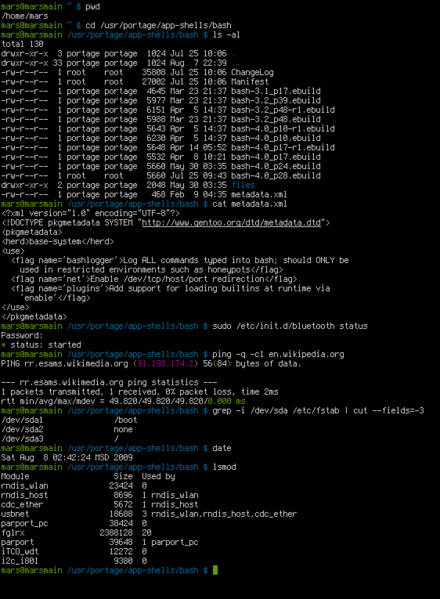
\includegraphics{img/440px-Bash_screenshot.png}

\section{What is the shell?}\label{what-is-the-shell}

The shell is a program on your computer whose job is to run other programs. Pseudo-synonyms are ``terminal'', ``command line'', and ``console''. There's a whole StackExchange thread on the differences (\href{https://askubuntu.com/questions/506510/what-is-the-difference-between-terminal-console-shell-and-command-line}{What is the difference between Terminal, Console, Shell, and Command Line?}), but I don't find it to be terribly enlightening. Your mileage may vary.

Many programmers spend lots of time in a shell, as opposed to in GUIs, because it is very fast, concise, and ubiquitous in their relevant computing environments. This is how all work was done before we got the mouse and GUIs.

The most common shell is \texttt{bash} and it gets thrown around as a proxy for ``shell'' sometimes, just like ``Coke'' and ``Kleenex'' are proxies for cola and tissues.

In Happy Git, sometimes we demo the use of a shell for certain tasks, like navigating the file system and doing Git operations, when we don't want to or can't use RStudio. Providing shell commands is also less ambiguous and less perishable than describing human interactions with a GUI.

\section{Starting the shell}\label{starting-the-shell}

\subsection{From within RStudio}\label{from-within-rstudio}

You can launch a shell from RStudio. This is often handy, because RStudio makes every effort to put you in a sane working directory, i.e.~in the current project.

There are two ways:

\begin{itemize}
\tightlist
\item
  \emph{Tools \textgreater{} Terminal} launches a shell within RStudio, graphically and process-wise. I believe this is usually what you want.
\item
  \emph{Tools \textgreater{} Shell \ldots{}} launches a shell external to RStudio.
\end{itemize}

\subsection{Outside of RStudio}\label{outside-of-rstudio}

\subsubsection{macOS}\label{macos-1}

The shell is often called the ``terminal'' on macOS, by which people mean Terminal.app. One way to launch is via Spotlight Search. Type Command + space and start typing ``terminal''. This process will something like so:

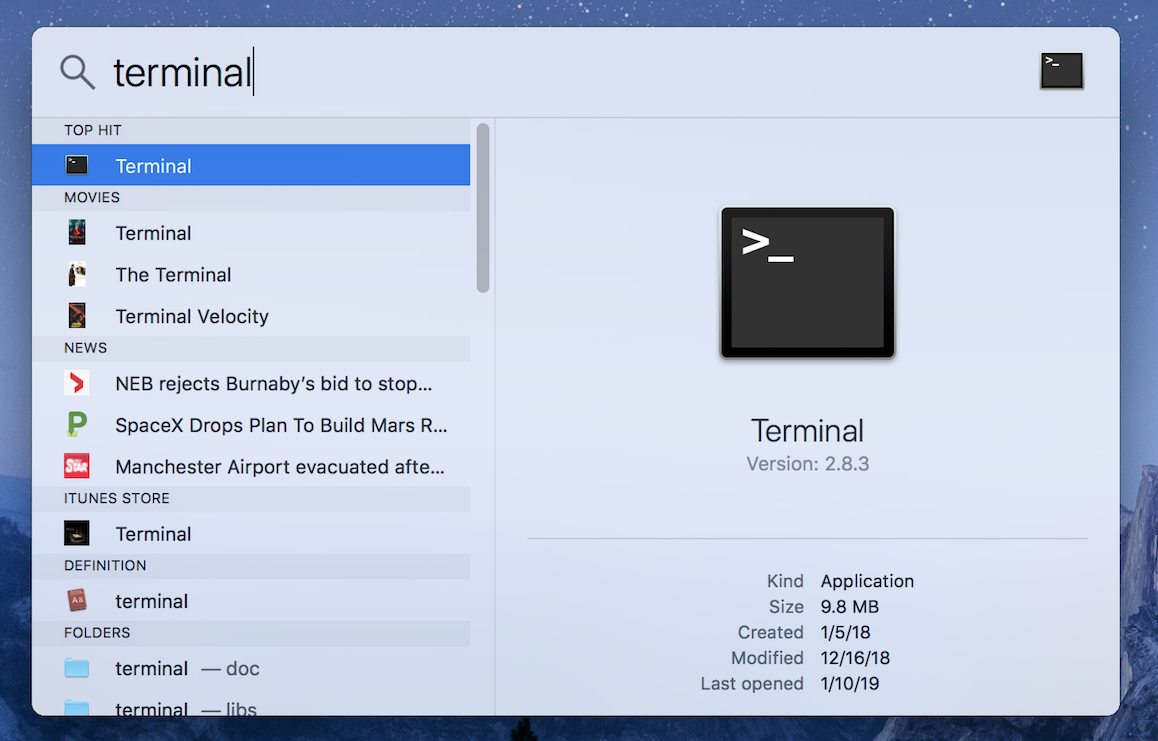
\includegraphics{img/terminal_mac_search.png}

Terminal.app is typically located at \emph{/Applications/Utilities/Terminal.app}.

Opening Terminal.app brings you to a bash shell opened to your home directory \texttt{\textasciitilde{}/}, which is shorthand for \texttt{/Users/YOURUSERNAME}. You should see something like this:

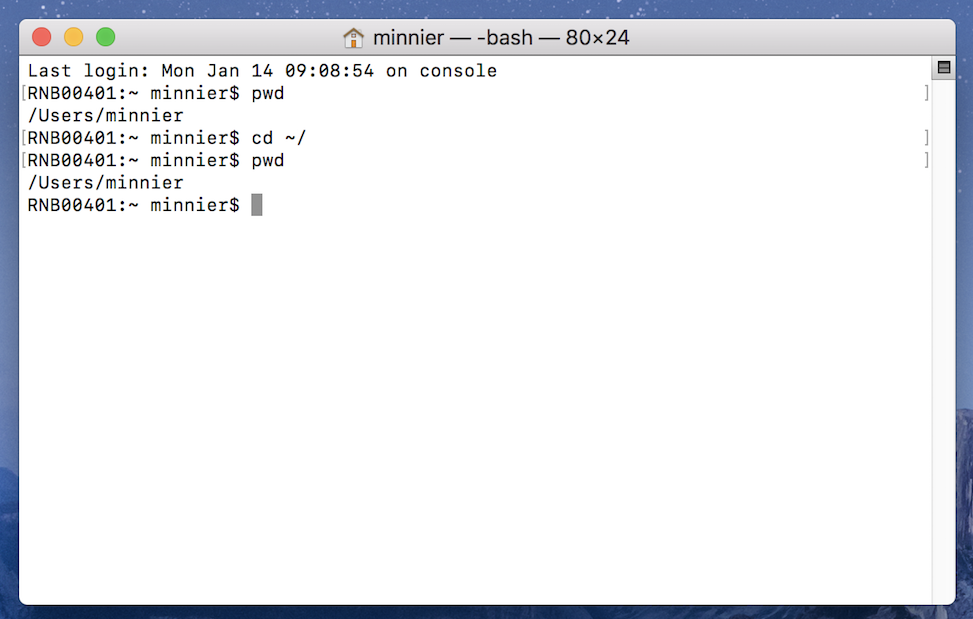
\includegraphics{img/terminal_mac.png}

If you have administrative rights on your computer, prefacing any command with \texttt{sudo} will allow you to run the command as an administrator. Expect to be challenged for your password. If you need to change administrative privileges or your password, see \href{https://support.apple.com/en-us/HT204012}{this article} from Apple.

\subsubsection{Windows}\label{windows-1}

We defer this until the next section, due to the more complex shell situation on Windows.

\section{Windows is special \ldots{} and not in a good way}\label{windows-shell-hell}

Windows is not the ideal platform for scientific computing and software development. A lot of the functionality is going to feel janky and strapped on. Because it is.

There are no fewer than 4 possible shells you can end up in. Unless you know better, you almost certainly want to be in a Git Bash shell, especially here in Happy Git.

Windows users will want to understand the different types of shell, how to launch them, and how to tell which one you're in.

\subsection{Git Bash}\label{git-bash}

\emph{TL;DR how to tell if you're in a Git Bash shell? Do this:}

\begin{Shaded}
\begin{Highlighting}[]
\ExtensionTok{$}\NormalTok{ echo }\VariableTok{$SHELL}
\ExtensionTok{/usr/bin/bash}
\end{Highlighting}
\end{Shaded}

Git Bash is a bash shell that ships with Git for Windows, which is \hyperref[install-git-windows]{the Happy Git way to install Git on Windows}. Therefore, you will not have Git Bash on your system until you install Git for Windows.

Git Bash is always the Windows shell we are targeting in Happy Git instructions.

RStudio should automatically detect the presence of Git Bash. You can inspect and influence this directly via \emph{Tools \textgreater{} Global Options \textgreater{} Terminal}. Unless you have good reason to do otherwise, you want to see ``Git Bash'' in the ``New terminals open with \ldots{}'' dropdown menu.

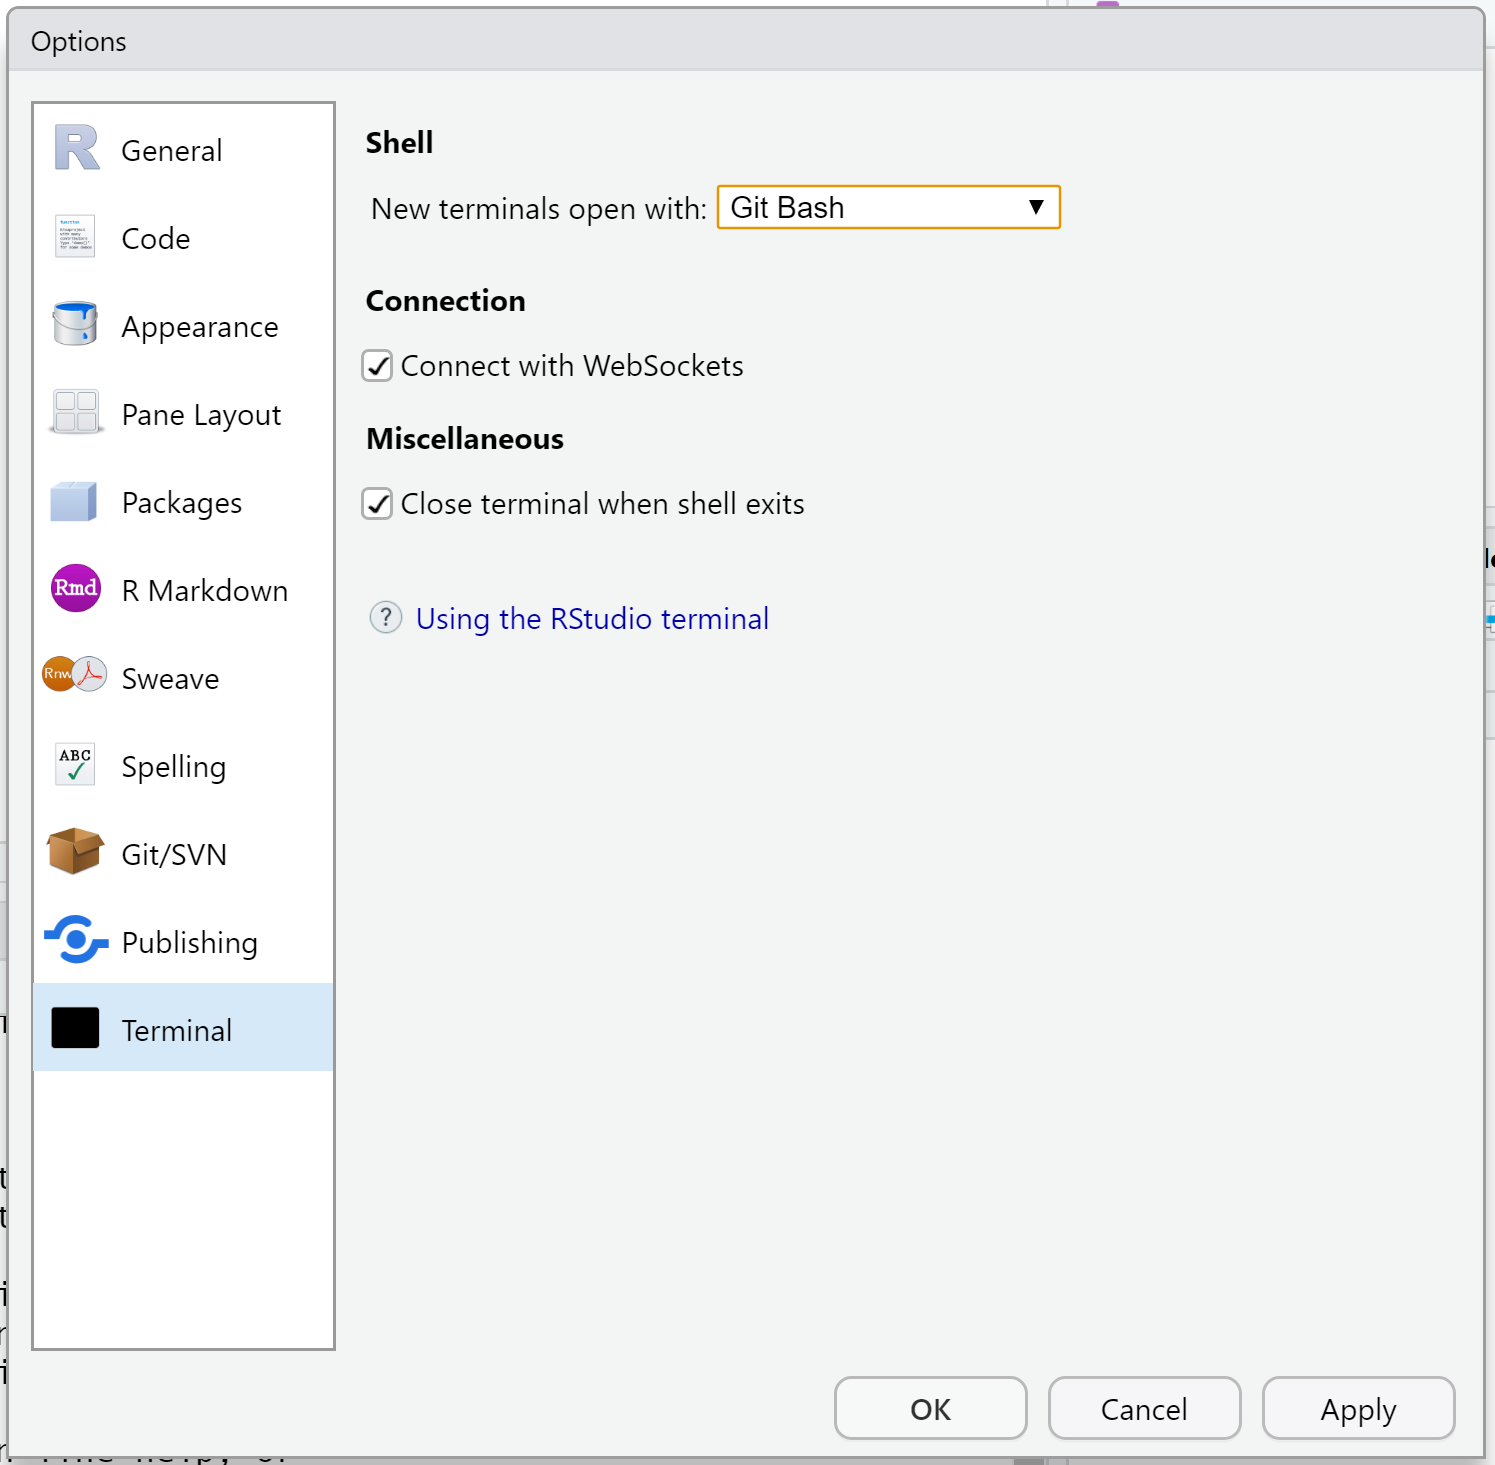
\includegraphics{img/git-bash-as-rstudio-terminal.png}

Troubleshooting tips:

\begin{itemize}
\tightlist
\item
  Restart RStudio. You need to restart all instances of RStudio after installing Git for Windows (+ Git Bash), in order for RStudio to auto-detect Git Bash.
\item
  Update RStudio. The shell handling in RStudio has improved dramatically over time, so older versions might not behave as described here.
\end{itemize}

\subsubsection{Accessing Git Bash outside of RStudio}\label{accessing-git-bash-outside-of-rstudio}

Sometimes you want to run Git Bash outside of RStudio. Here's the easiest way: click the ``Git'' menu in the Windows menu and select ``Git Bash''.

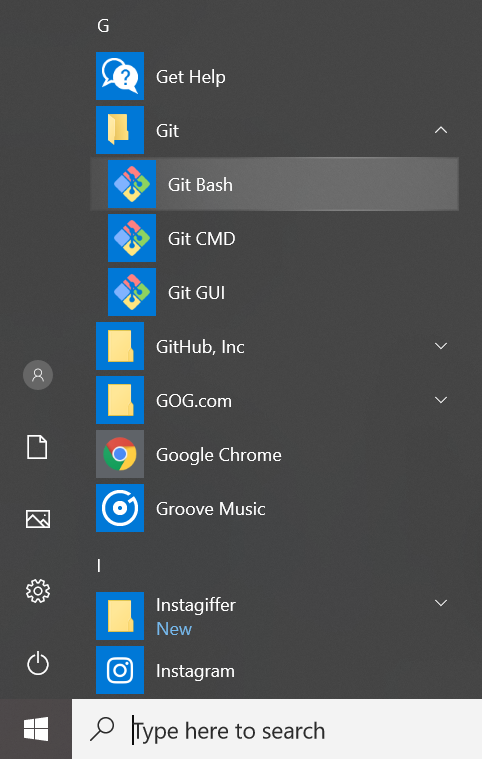
\includegraphics{img/2019-01_git_bash_windows.png}

A Git Bash shell running outside of RStudio looks something like this:

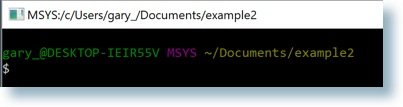
\includegraphics{img/2018-01-15_git-bash.png}

Notice \texttt{MSYS} in the title bar. You might also see \texttt{MINGW64}.

Sometimes you need to run Git Bash as administrator, e.g.~to run with higher privileges. Easiest way: click the ``Git'' menu in the Windows menu and \emph{right-click} on ``Git Bash''. This reveals a submenu. Select ``more'' and then ``Run as administrator''.

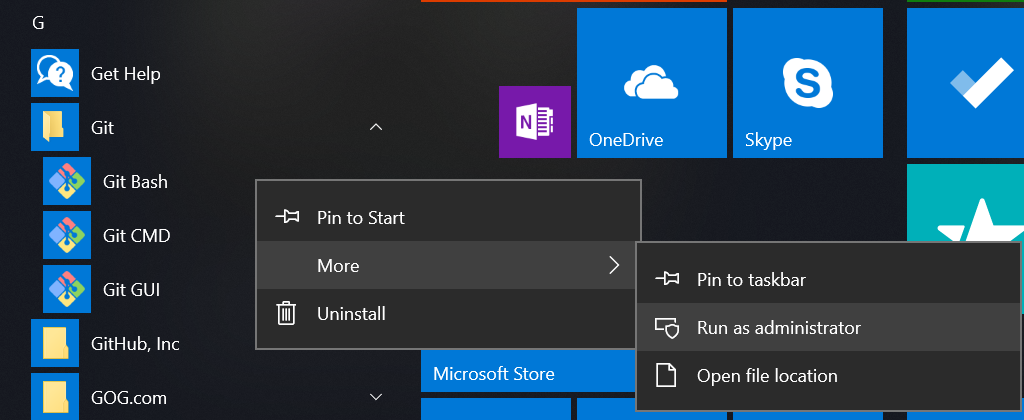
\includegraphics{img/2019-01-git-windows-administrator.png}

\subsection{Command prompt}\label{command-prompt}

\emph{TL;DR how to tell if you're in Command Prompt? Do this:}

\begin{Shaded}
\begin{Highlighting}[]
\ExtensionTok{C:\textbackslash{}Users\textbackslash{}jenny}\OperatorTok{\textgreater{}}\NormalTok{echo \%COMSPEC\%}
\ExtensionTok{C:\textbackslash{}WINDOWS\textbackslash{}system32\textbackslash{}cmd.exe}
\end{Highlighting}
\end{Shaded}

This is the native Windows command line interpreter. It's rarely what you want, especially for the work described in Happy Git.

A Command Prompt session running outside of RStudio looks something like this:

\includegraphics{img/2018-01-15_command-prompt.png}

Notice the \texttt{cmd.exe} in the title bar, although it is not \emph{always} present. You might also see ``Command Prompt''.

If you get an error message such as \texttt{\textquotesingle{}pwd\textquotesingle{}\ is\ not\ recognized\ as\ an\ internal\ or\ external\ command,\ operable\ program\ or\ batch\ file.} from a shell command, that suggests you have somehow launched into \texttt{cmd.exe} when you did not mean to.

\subsection{PowerShell}\label{powershell}

\emph{TL;DR how to tell if you're in PowerShell? Do this:}

\begin{Shaded}
\begin{Highlighting}[]
\ExtensionTok{PS}\NormalTok{ C:}\DataTypeTok{\textbackslash{}U}\NormalTok{sers}\DataTypeTok{\textbackslash{}j}\NormalTok{enny}\OperatorTok{\textgreater{}}\NormalTok{ Get{-}ChildItem Env:ComSpec}

\ExtensionTok{Name}\NormalTok{                           Value}
\ExtensionTok{{-}{-}{-}{-}}                           \AttributeTok{{-}{-}{-}{-}{-}}
\ExtensionTok{ComSpec}\NormalTok{                        C:}\DataTypeTok{\textbackslash{}W}\NormalTok{INDOWS}\DataTypeTok{\textbackslash{}s}\NormalTok{ystem32}\DataTypeTok{\textbackslash{}c}\NormalTok{md.exe}
\end{Highlighting}
\end{Shaded}

PowerShell is yet another Windows shell, a more modern successor to Command Prompt. It's also rarely what you want, especially for the work described in Happy Git.

A PowerShell session running outside of RStudio looks something like this:

\includegraphics{img/2018-01-15_power-shell.png}

Notice the \texttt{powershell.exe} in the title bar.

\subsection{Bash via Windows Services for Linux}\label{bash-via-windows-services-for-linux}

\emph{TL;DR how to tell if you're in Bash via WSL? Do this:}

\begin{Shaded}
\begin{Highlighting}[]
\ExtensionTok{$}\NormalTok{ echo }\VariableTok{$SHELL}
\ExtensionTok{/bin/bash}
\end{Highlighting}
\end{Shaded}

In 2016, Microsoft launched the Windows Subsystem for Linux (WSL), ``a new Windows 10 feature that enables you to run native Linux command-line tools directly on Windows''. Overall, this is a fantastic development. However, at the time of writing (January 2019), you will only have this if you're running Windows 10 64-bit and have chosen to \href{https://docs.microsoft.com/en-us/windows/wsl/install-win10}{install the optional WSL system component}. Therefore, I expect only keeners to have this and, in that case, you probably don't need this chapter.

A WSL bash shell running outside of RStudio looks something like this:

\includegraphics{img/2018-01-15_bash-windows-services-for-linux.png}

FYI Microsoft also refers to WSL as Bash on Ubuntu on Windows.

\subsubsection{Windows bottom line}\label{windows-bottom-line}

When in doubt, you probably want to be in a Git Bash shell.

\section{Basic shell commands}\label{basic-shell-commands}

The most basic commands are listed below:

\begin{itemize}
\tightlist
\item
  \href{https://en.wikipedia.org/wiki/Pwd}{\texttt{pwd}} (\textbf{p}rint \textbf{w}orking \textbf{d}irectory). Shows directory or ``folder'' you are currently operating in. This is not necessarily the same as the \texttt{R} working directory you get from \texttt{getwd()}.
\item
  \href{https://en.wikipedia.org/wiki/Ls}{\texttt{ls}} (\textbf{l}i\textbf{s}t files). Shows the files in the current working directory. This is equivalent to looking at the files in your Finder/Explorer/File Manager. Use \texttt{ls\ -a} to also list hidden files, such as \texttt{.Rhistory} and \texttt{.git}.
\item
  \href{https://en.wikipedia.org/wiki/Cd_(command)}{\texttt{cd}} (\textbf{c}hange \textbf{d}irectory). Allows you to navigate through your directories by changing the shell's working directory. You can navigate like so:

  \begin{itemize}
  \tightlist
  \item
    go to subdirectory \texttt{foo} of current working directory: \texttt{cd\ foo}
  \item
    go to parent of current working directory: \texttt{cd\ ..}
  \item
    go to your ``home'' directory: \href{http://tilde.club/~ford/tildepoint.jpg}{\texttt{cd\ \textasciitilde{}}} or simply \texttt{cd}
  \item
    go to directory using absolute path, works regardless of your current working directory: \texttt{cd\ /home/my\_username/Desktop}. Windows uses a slightly different syntax with the slashes between the folder names reversed, \texttt{\textbackslash{}}, e.g.~\texttt{cd\ C:\textbackslash{}Users\textbackslash{}MY\_USERNAME\textbackslash{}Desktop}.

    \begin{itemize}
    \tightlist
    \item
      Pro tip 1: Dragging and dropping a file or folder into the terminal window will paste the absolute path into the window.
    \item
      Pro tip 2: Use the \texttt{tab} key to autocomplete unambiguous directory and file names. Hit \texttt{tab} twice to see all ambiguous options.
    \end{itemize}
  \end{itemize}
\item
  Use arrow-up and arrow-down to repeat previous commands. Or search for previous commands with \texttt{CTRL} + \texttt{r}.
\end{itemize}

A few Git commands:

\begin{itemize}
\tightlist
\item
  \texttt{git\ status} is the most used git command and informs you of your current branch, any changes or untracked files, and whether you are in sync with your remotes.
\item
  \texttt{git\ remote\ -v} lists all remotes. Very useful for making sure \texttt{git} knows about your remote and that the remote address is correct.
\item
  \texttt{git\ remote\ add\ origin\ GITHUB\_URL} adds the remote \texttt{GITHUB\_URL} with nickname \texttt{origin}.
\item
  \texttt{git\ remote\ set-url\ origin\ GITHUB\_URL} changes the remote url of \texttt{origin} to \texttt{GITHUB\_URL}. This way you can fix typos in the remote url.
\item
  \emph{Feel free to suggest other commands that deserve listing in a \href{https://github.com/jennybc/happy-git-with-r/issues}{GitHub issue}.}
\end{itemize}

\chapter{Comic relief}\label{comic-relief}

It's not you, it's Git!

If you're not crying already, these fictional-but-realistic Git man pages should do the trick:

\begin{itemize}
\tightlist
\item
  \href{http://git-man-page-generator.lokaltog.net}{git-man-page-generator}
\item
  And, of course, the underlying source is also available on GitHub:

  \begin{itemize}
  \tightlist
  \item
    \url{https://github.com/Lokaltog/git-man-page-generator}
  \end{itemize}
\end{itemize}

If you can tolerate adult and often offensive language, you might enjoy:

\begin{itemize}
\tightlist
\item
  \url{http://www.commitlogsfromlastnight.com}
\item
  \url{http://ohshitgit.com/}
\end{itemize}

Your commits will look more glorious scrolling by Star Wars style:

\begin{itemize}
\tightlist
\item
  \url{http://starlogs.net}
\item
  \url{http://starlogs.net/\#jennybc/googlesheets}
\item
  Do this for any repo: \texttt{http://starlogs.net/\#USER/REPO}
\end{itemize}

\chapter{Resources}\label{resources}

We practice what we preach! This site is created with Git and R markdown, using the \href{https://github.com/rstudio/bookdown/}{\texttt{bookdown}} package. Go ahead and \href{https://github.com/jennybc/happy-git-with-r}{peek behind the scenes}.

Long-term, you should understand more about what you are doing. Rote clicking in RStudio may be a short-term survival method but won't work for long.

\begin{itemize}
\item
  \href{https://speakerdeck.com/alicebartlett/git-for-humans}{Git for Humans} is a great set of slides by \href{https://alicebartlett.co.uk}{Alice Bartlett}, originally delivered in 2016 at UX Brighton.
\item
  \href{https://www.manning.com/books/git-in-practice}{Git in Practice} by Mike McQuaid is an more approachable book, probably better than Pro Git (below) for most people starting out. Ancillary materials \href{https://github.com/MikeMcQuaid/GitInPractice}{on GitHub}.
\item
  The book \href{http://git-scm.com/book}{Pro Git} is fantastic and comprehensive.
\item
  \href{https://ohmygit.org/}{Oh My Git!} is a free and open source interactive game for learning Git. It's very beginner friendly, using a graph to visualise the worktree. Lessons can be completed using a playing card interface in addition to the built-in command line, which is there for when users become more comfortable.
\item
  \href{https://training.github.com}{GitHub's own training materials} may be helpful. They also point to \href{https://help.github.com/articles/what-are-other-good-resources-for-learning-git-and-github}{many other resources}
\item
  Find a powerful Git client (chapter \ref{git-client}) if you'd like to minimize your usage of Git from the command line.
\item
  Ten Simple Rules for Taking Advantage of Git and GitHub \url{http://journals.plos.org/ploscompbiol/article?id=10.1371/journal.pcbi.1004947}
\item
  RStudio's guide \href{https://support.rstudio.com/hc/en-us/articles/200532077-Version-Control-with-Git-and-SVN}{Version Control with Git and SVN}
\item
  The book \emph{\href{http://shop.oreilly.com/product/0636920018025.do}{Team Geek}} has insightful advice for the human and collaborative aspects of version control. It proposes Git strategies suited to different characteristics of teams.
\end{itemize}

\phantomsection\label{refs}
\begin{CSLReferences}{1}{0}
\bibitem[\citeproctext]{ref-git-for-humans}
Bartlett, Alice. 2016. {``Git for Humans.''} Financial Times, London; Talk at UX Brighton. \url{https://speakerdeck.com/alicebartlett/git-for-humans}.

\bibitem[\citeproctext]{ref-ten-simple-rules-git}
Perez-Riverol, Yasset, Laurent Gatto, Rui Wang, Timo Sachsenberg, Julian Uszkoreit, Felipe da Veiga Leprevost, Christian Fufezan, et al. 2016. {``Ten Simple Rules for Taking Advantage of Git and GitHub.''} \emph{PLOS Computational Biology} 12 (7): 1--11. \url{https://doi.org/10.1371/journal.pcbi.1004947}.

\bibitem[\citeproctext]{ref-Ram2013}
Ram, Karthik. 2013. {``Git Can Facilitate Greater Reproducibility and Increased Transparency in Science.''} \emph{Source Code for Biology and Medicine} 8 (1): 7. \url{https://doi.org/10.1186/1751-0473-8-7}.

\bibitem[\citeproctext]{ref-r-pkgs-book}
Wickham, Hadley. 2015. \emph{R Packages}. 1st ed. O'Reilly Media, Inc.

\bibitem[\citeproctext]{ref-knitr-book}
Xie, Yihui. 2015. \emph{Dynamic Documents with {R} and Knitr}. 2nd ed. Boca Raton, Florida: Chapman; Hall/CRC. \url{http://yihui.name/knitr/}.

\bibitem[\citeproctext]{ref-R-bookdown}
---------. 2024. \emph{Bookdown: Authoring Books and Technical Documents with r Markdown}. \url{https://github.com/rstudio/bookdown}.

\end{CSLReferences}

\end{document}
